\documentclass[11pt]{article}

\usepackage[a4paper]{geometry}
\geometry{left=2.0cm,right=2.0cm,top=2.5cm,bottom=2.5cm}

\usepackage{ctex} % 支持中文的LaTeX宏包
\usepackage{amsmath,amsfonts,graphicx,subfigure,amssymb,bm,amsthm,mathrsfs,mathtools,breqn} % 数学公式和符号的宏包集合
\usepackage{algorithm,algorithmicx} % 算法和伪代码的宏包
\usepackage[noend]{algpseudocode} % 算法和伪代码的宏包
\usepackage{fancyhdr} % 自定义页眉页脚的宏包
\usepackage[framemethod=TikZ]{mdframed} % 创建带边框的框架的宏包
\usepackage{fontspec} % 字体设置的宏包
\usepackage{adjustbox} % 调整盒子大小的宏包
\usepackage{fontsize} % 设置字体大小的宏包
\usepackage{tikz} % 绘制图形和使用颜色的宏包
\usetikzlibrary{arrows.meta,positioning} % TikZ箭头库和定位库
\usepackage{float} % 支持[H]浮动体位置参数
\usepackage{multicol} % 多栏排版的宏包
\usepackage{multirow} % 表格中合并单元格的宏包
\usepackage{pdfpages} % 插入PDF文件的宏包
\RequirePackage{listings} % 在文档中插入源代码的宏包
\usepackage{wrapfig} % 文字绕排图片的宏包
\usepackage{bigstrut,multirow,rotating} % 支持在表格中使用特殊命令的宏包
\usepackage{booktabs} % 创建美观的表格的宏包
\usepackage{circuitikz} % 绘制电路图的宏包
\usepackage{hyperref} % 创建超链接的宏包
% \usepackage{subcaption} % 支持子图标题的宏包
\usepackage[inline]{enumitem} % 自定义列表格式的宏包，支持行内列表

\definecolor{dkgreen}{rgb}{0,0.6,0}
\definecolor{gray}{rgb}{0.5,0.5,0.5}
\definecolor{mauve}{rgb}{0.58,0,0.82}
\lstset{
  frame=tb,
  aboveskip=3mm,
  belowskip=3mm,
  showstringspaces=false,
  columns=flexible,
  framerule=1pt,
  rulecolor=\color{gray!35},
  backgroundcolor=\color{gray!5},
  basicstyle={\small\ttfamily},
  numbers=none,
  numberstyle=\tiny\color{gray},
  keywordstyle=\color{blue},
  commentstyle=\color{dkgreen},
  stringstyle=\color{mauve},
  breaklines=true,
  breakatwhitespace=true,
  tabsize=3,
}


\usepackage[capitalize]{cleveref}
\Crefname{section}{Section}{Sections}
\Crefname{table}{Table}{Tables}
\crefname{table}{Table.}{Tabs.}

\setmainfont{Palatino Linotype}
\setCJKmainfont{SimSun}[BoldFont=SimHei, ItalicFont=KaiTi]
\setCJKsansfont{SimHei}
\setCJKmonofont{FangSong}
\punctstyle{kaiming}
% 偏好的几个字体, 可以根据需要自行加入字体ttf文件并调用

% Restore standard emphasis to avoid requiring an undefined environment (kaishu).
% The original redefinition used an environment `kaishu` which is not defined
% in a default ctex setup and causes compilation errors. Use \textit for
% emphasis which works across engines.
\renewcommand{\emph}[1]{\textit{#1}}

%改这里可以修改实验报告表头的信息
\newcommand{\experiName}{傅里叶光学实验}
\newcommand{\supervisor}{左站春}
\newcommand{\name}{邓思豪}
\newcommand{\studentNum}{2023K8009909008}
\newcommand{\class}{3}
\newcommand{\group}{01}
\newcommand{\seat}{5}
\newcommand{\dateYear}{2025}
\newcommand{\dateMonth}{11}
\newcommand{\dateDay}{5}
\newcommand{\room}{西实201}
\newcommand{\others}{$\square$}


\begin{document}



\begin{center}
    \LARGE \bf 《\, 基\, 础\, 物\, 理\, 实\, 验\, 》\, 实\, 验\, 报\, 告
\end{center}

\begin{center}
    \noindent \emph{实验名称}\underline{\makebox[25em][c]{\experiName}}
    \emph{指导教师}\underline{\makebox[8em][c]{\supervisor}}\\
    \emph{姓名}\underline{\makebox[6em][c]{\name}} 
    % 如果名字比较长, 可以修改box的长度"6em"
    \emph{学号}\underline{\makebox[10em][c]{\studentNum}}
    \emph{分班分组及座号} \underline{\makebox[5em][c]{\class \ -\ \group \ -\ \seat }\emph{号}} （\emph{例}:\, 1\,-\,04\,-\,5\emph{号}）\\
    \emph{实验日期} \underline{\makebox[3em][c]{\dateYear}}\emph{年}
    \underline{\makebox[2em][c]{\dateMonth}}\emph{月}
    \underline{\makebox[2em][c]{\dateDay}}\emph{日}
    \emph{实验地点}\underline{{\makebox[6em][c]\room}}
    \emph{调课/补课} \underline{\makebox[3em][c]{\others\ 是}}
    \emph{成绩评定} \underline{\hspace{5em}}
    {\noindent}
    \rule[8pt]{17cm}{0.2em}
\end{center}

\section{实验原理}

\subsection{薄透镜焦距的测定实验原理}

透镜是光学仪器的基本元件，\textbf{薄透镜}指中心厚度远小于焦距或曲率半径的透镜，焦距是其核心参数（决定成像的大小、虚实、倒正），分为会聚的凸透镜与发散的凹透镜。

\subsubsection{成像公式法}
近轴光线条件下，薄透镜成像的高斯公式为：
\begin{equation}
\frac{1}{s} + \frac{1}{s'} = \frac{1}{f}
\end{equation}
置于空气中时，焦距为：
\begin{equation}
f = \frac{ss'}{s + s'}
\end{equation}
式中：$s$为物距（实物$>0$、虚物$<0$），$s'$为像距（实像$>0$、虚像$<0$），$f$为焦距（凸透镜$>0$、凹透镜$<0$），均以光心为原点。

凸透镜物距$u$与像距$v$的成像规律见表\ref{tab:imaging_rule}：
\begin{table}[H]
\centering
\caption{凸透镜成像规律}
\label{tab:imaging_rule}
\begin{tabular}{|c|c|c|c|c|c|}
\hline
物距$u$ & 倒/正立 & 放/缩小 & 实/虚像 & 像距$v$ & 应用 \\
\hline
$u>2f$ & 倒立 & 缩小 & 实像 & $f<v<2f$ & 照相机 \\
\hline
$u=2f$ & 倒立 & 等大 & 实像 & $v=2f$ & - \\
\hline
$f<u<2f$ & 倒立 & 放大 & 实像 & $v>2f$ & 投影仪 \\
\hline
$u=f$ & \multicolumn{4}{c|}{不成像} & - \\
\hline
$u<f$ & 正立 & 放大 & 虚像 & - & 放大镜 \\
\hline
\end{tabular}
\end{table}

\begin{figure}[H]
\centering
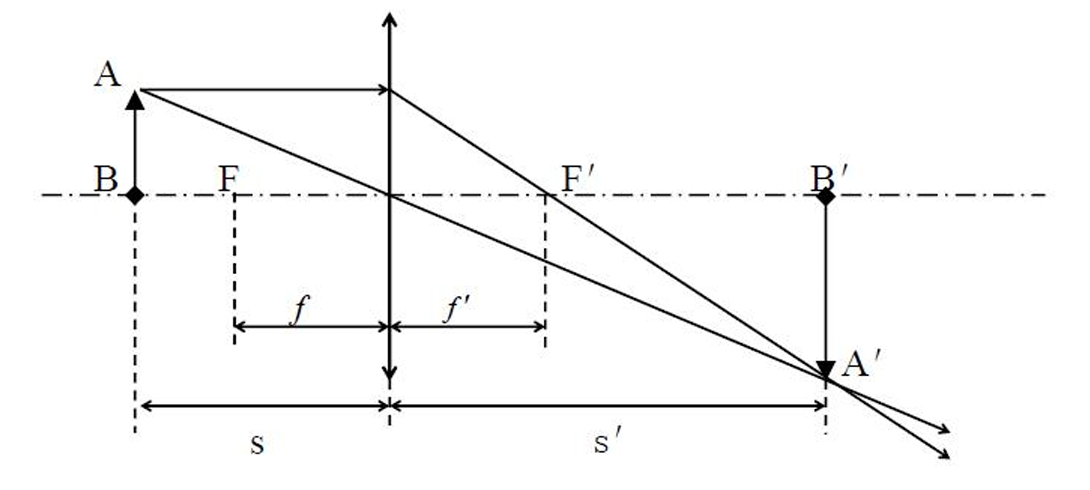
\includegraphics[width=0.8\textwidth]{imaging1.png}
\caption{成像法测定凸透镜焦距}
\label{fig:imaging1}
\end{figure}

\begin{figure}[H]
    \centering
    \subfigure[阿贝尔成像光路示意图]{
        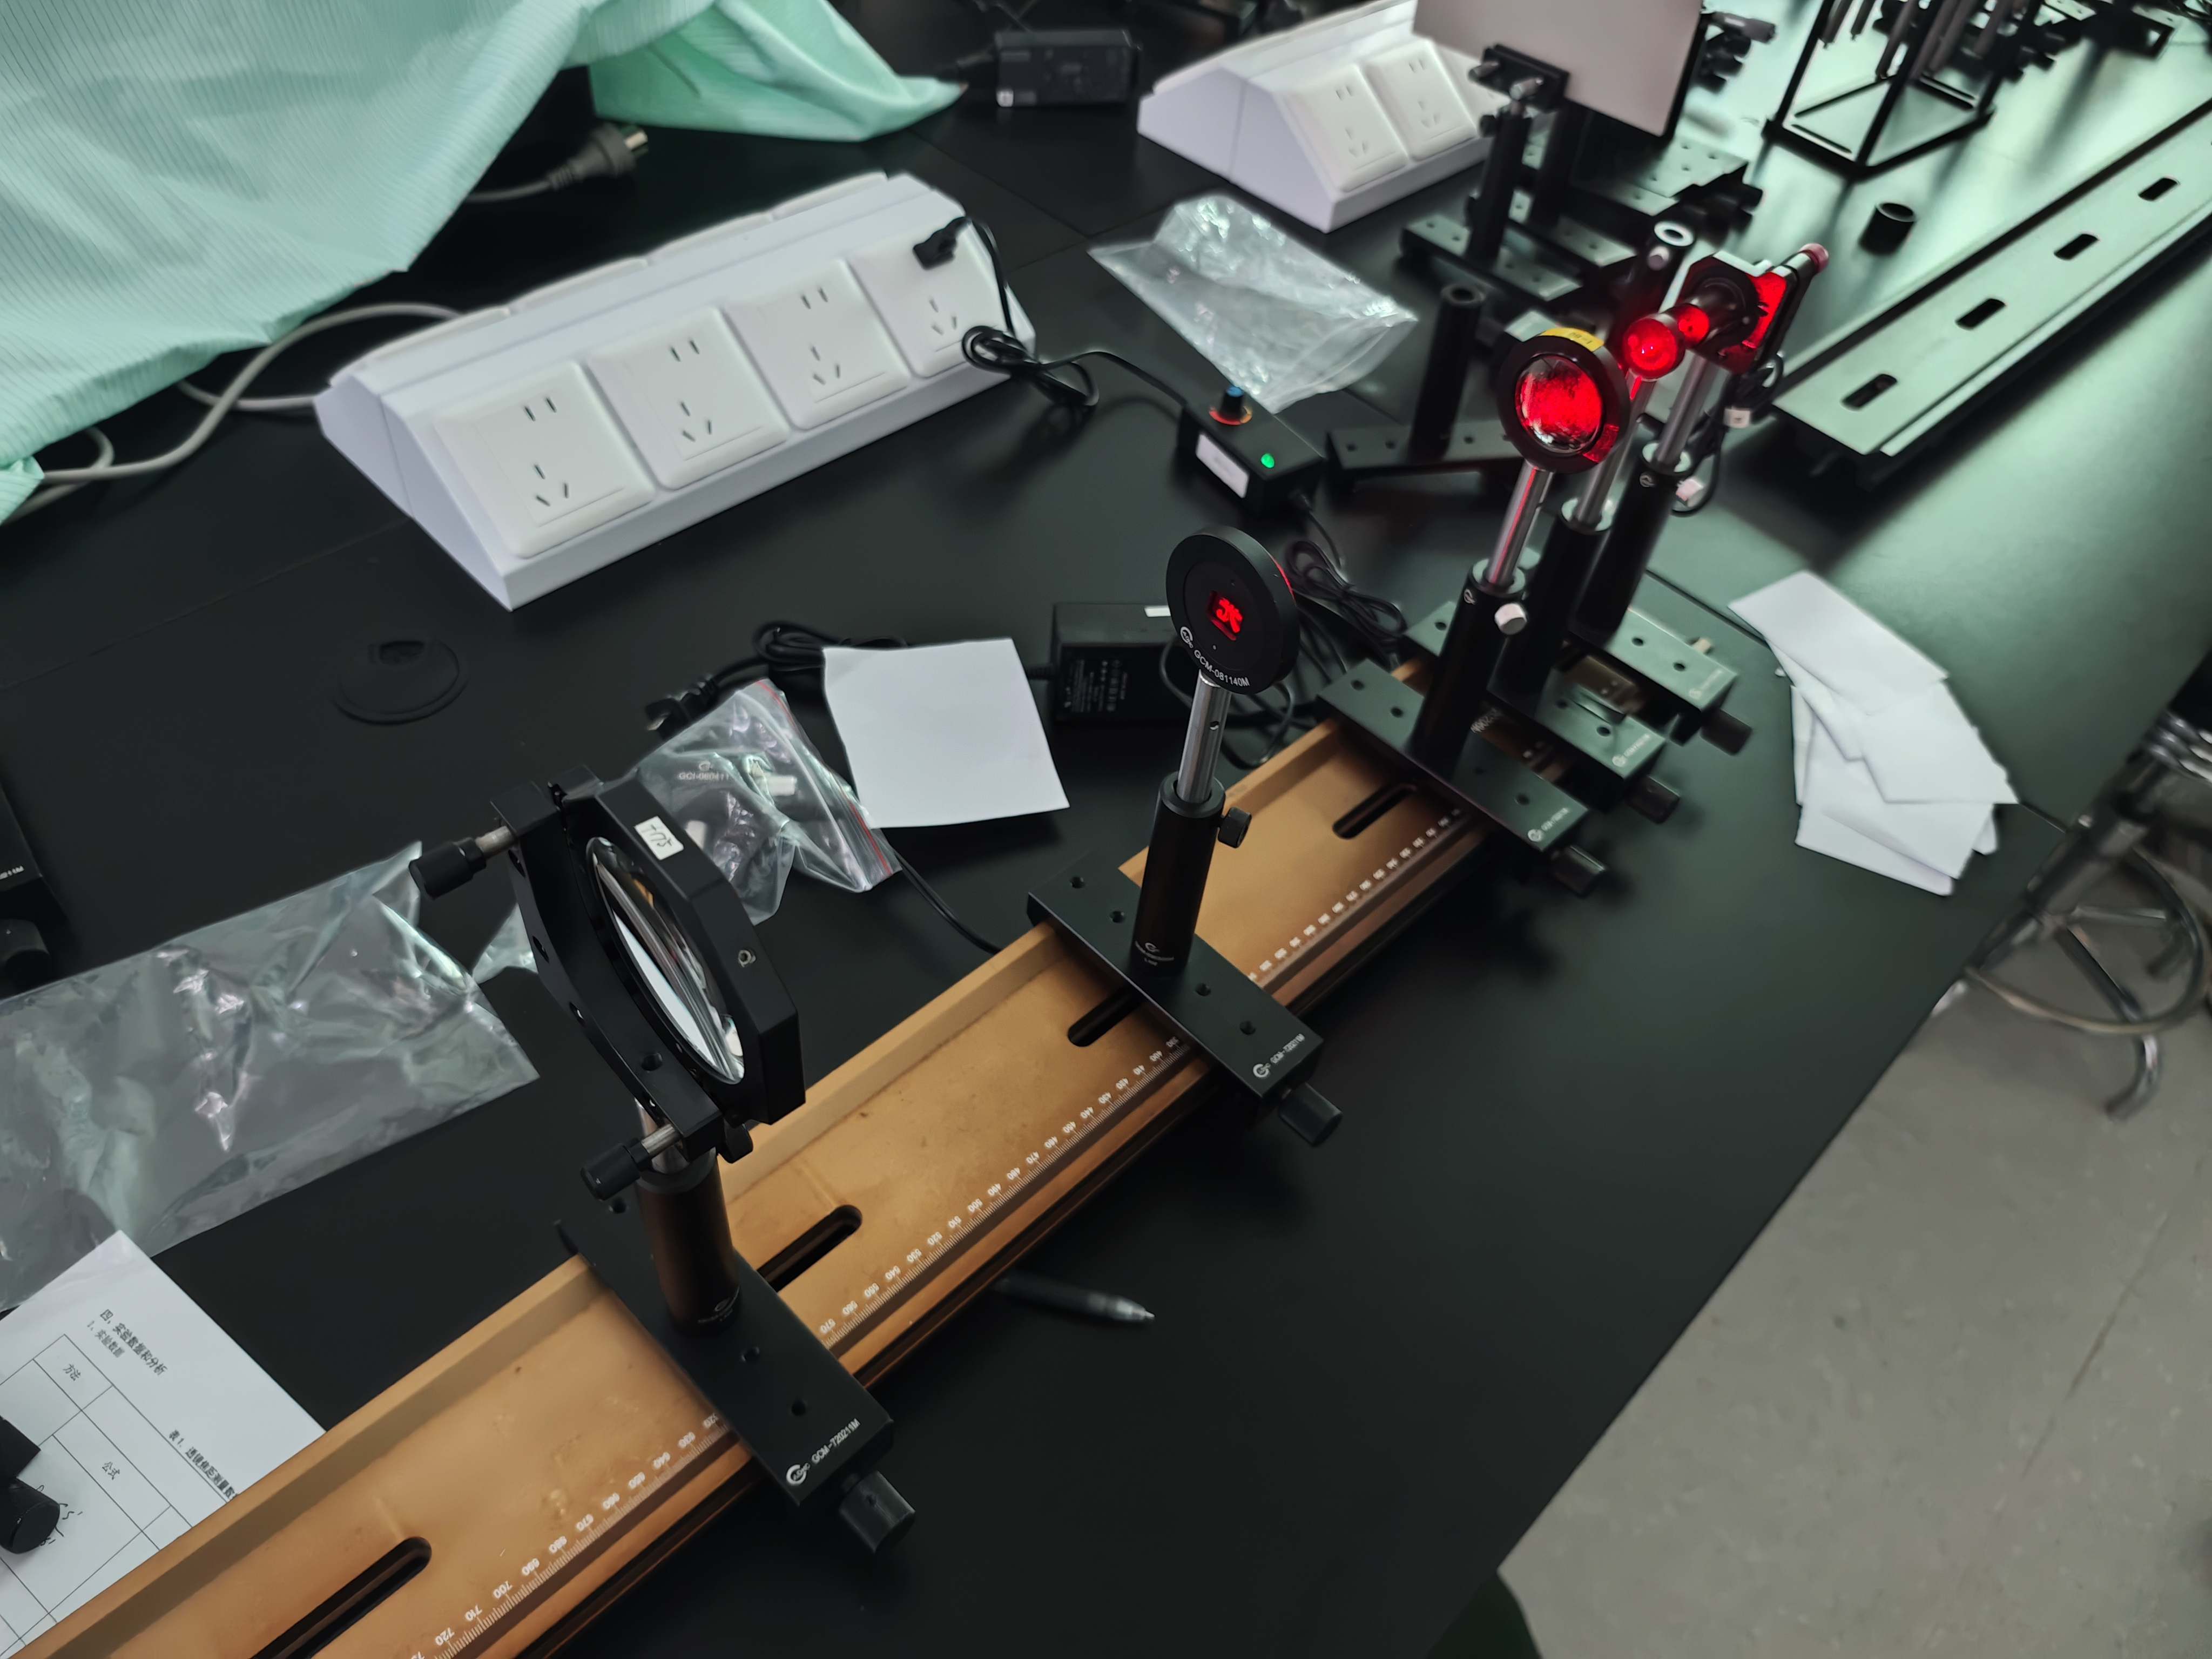
\includegraphics[width=0.4\textwidth]{fig 16a.jpg}
    }
    \hspace{0.05\textwidth}
    \subfigure[成像图样]{
        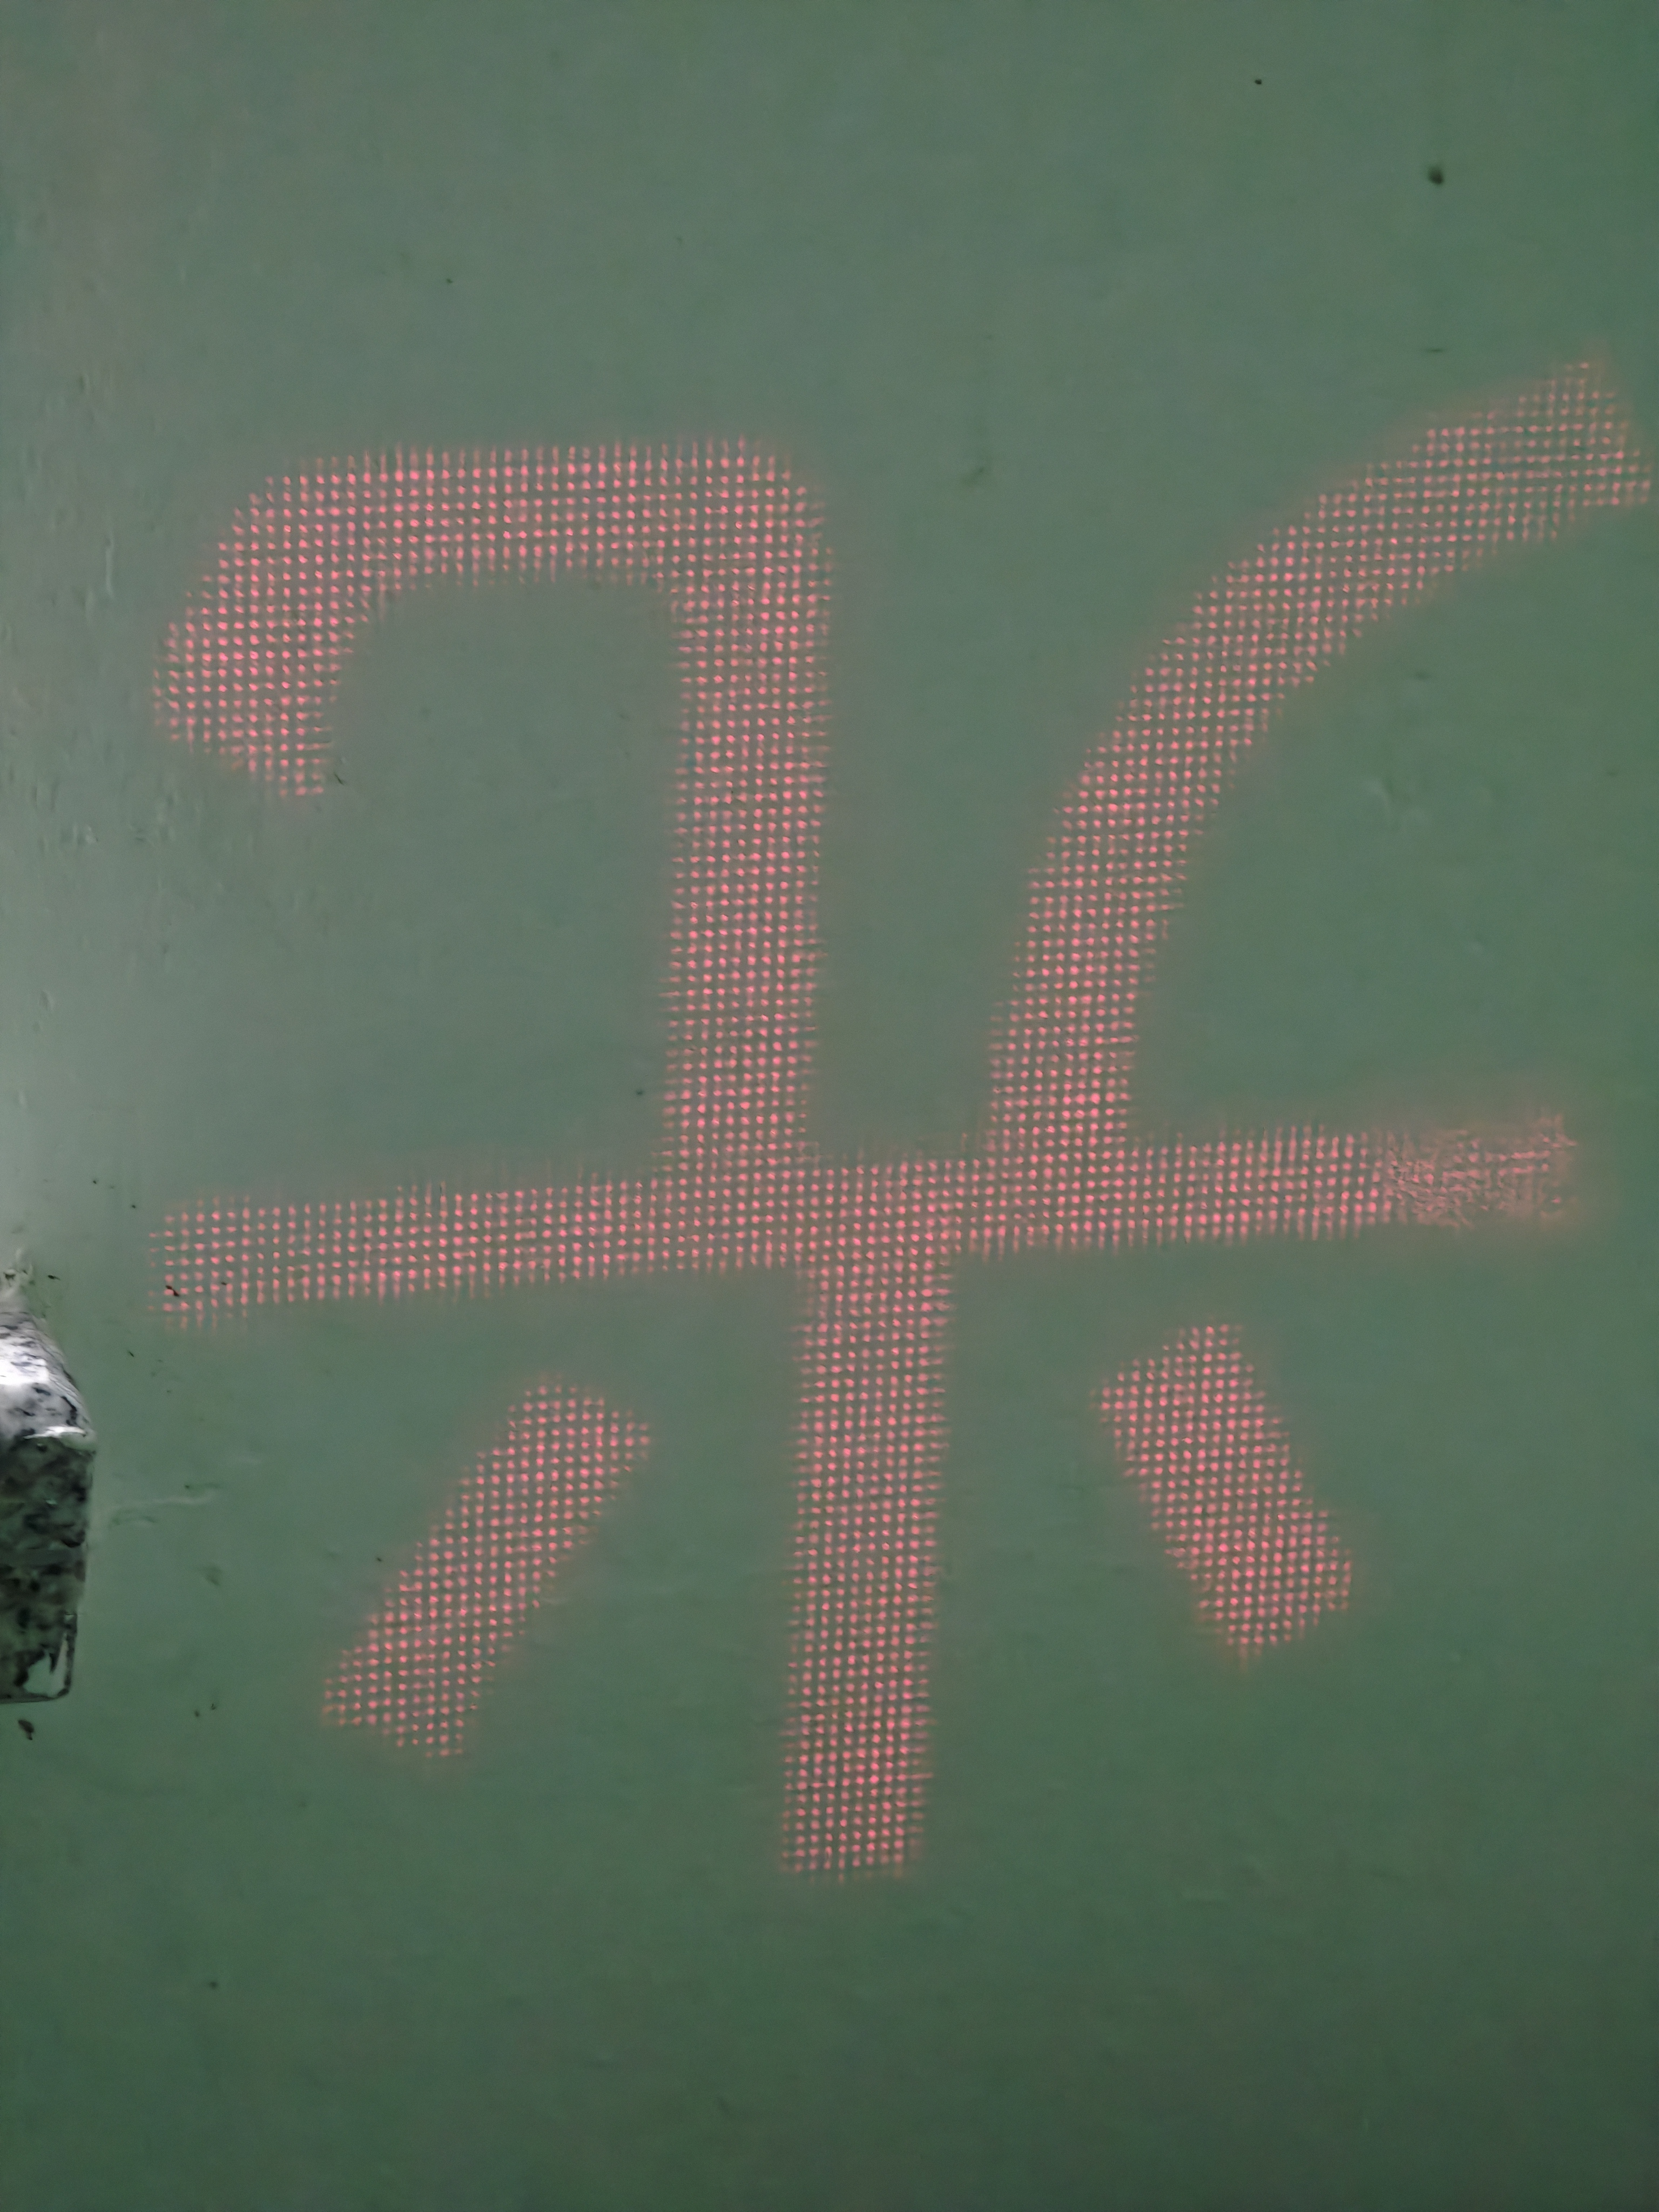
\includegraphics[width=0.4\textwidth]{fig 16b.jpg}
    }
    \caption{阿贝尔成像实验图}
\end{figure}

\begin{equation}
f = \frac{D^2 - d^2}{4D}
\end{equation}

\begin{figure}[H]
\centering
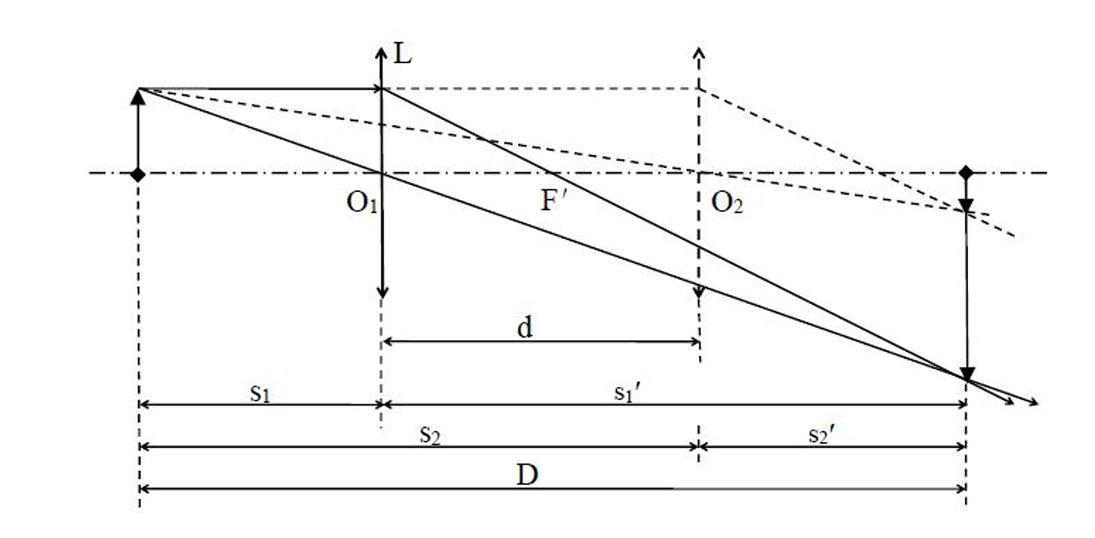
\includegraphics[width=0.8\textwidth]{double_imaging.png}
\caption{二次成像法测定凸透镜焦距}
\label{fig:double_imaging}
\end{figure}


\subsubsection{自准直法}
待测透镜一侧置物屏$AB$，另一侧置平面镜$M$。当$AB$位于透镜焦平面时，物点光线经透镜后变为平行光，经平面镜反射回透镜，会聚于原物屏，形成\textbf{等大倒立实像}，此时物屏到透镜的距离即为焦距$f$。

\begin{figure}[H]
\centering
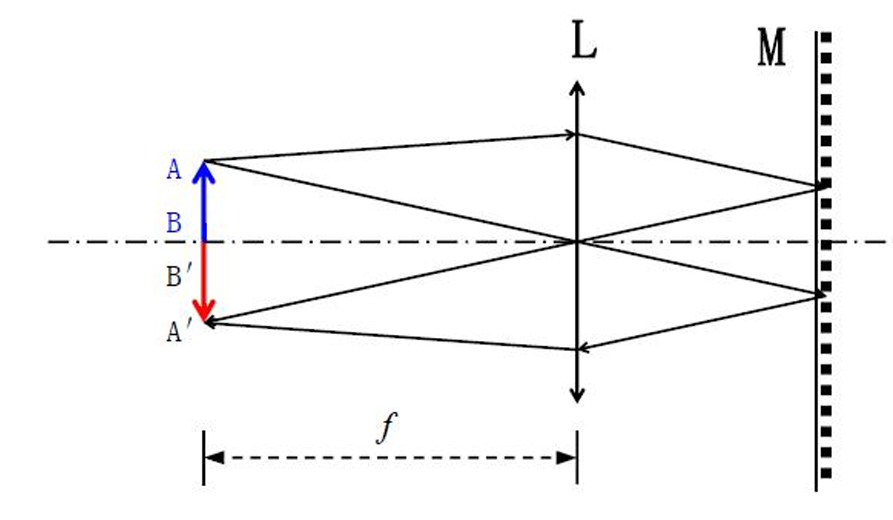
\includegraphics[width=0.8\textwidth]{autocollimation.png}
\caption{自准直法测定凸透镜焦距}
\label{fig:autocollimation}
\end{figure}


\subsubsection{凹透镜焦距测定（辅助透镜法）}
先由凸透镜$L_1$使物$AB$成实像$A'B'$，在$L_1$与$A'B'$间放入凹透镜$L_2$，使$A'B'$作为$L_2$的虚物，成实像$A''B''$。测$L_2$到$A'B'$的距离$s_2$（虚物，$s_2<0$）、到$A''B''$的距离$s_2'$（实像，$s_2'>0$），则凹透镜焦距：
\begin{equation}
f_2' = \frac{s_2s_2'}{s_2 + s_2'}
\end{equation}

\begin{figure}[H]
\centering
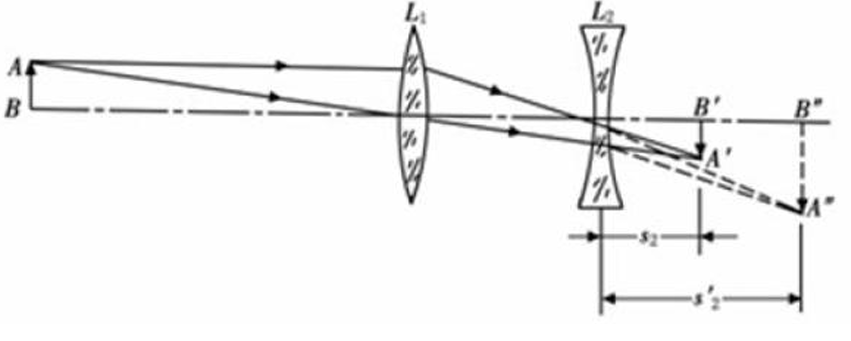
\includegraphics[width=0.8\textwidth]{concave_lens.png}
\caption{凹透镜焦距的测定}
\label{fig:concave_lens}
\end{figure}

\subsection{阿贝成像原理}
阿贝成像是傅里叶光学中最基本且直观的实验现象，它深刻揭示了波前传播过程中，透镜作用下频谱面的物理意义与存在性。阿贝成像原理的提出，在时间维度和物理概念上均处于传统几何光学与现代波动光学（基于波前传递的光场传播理论）之间，为现代光学的概念体系奠定了重要基础。

\subsubsection{成像理论的演进对比}
传统光学、阿贝成像原理与现代光学对成像过程的理解存在显著差异，其物理图像可概括如下：

基于几何光学的传统模型（如图\ref{fig:imaging_models}a）将"物"视为光源，认为"物"与"像"存在一一对应的映射关系，透镜的核心作用是实现光线的重新聚焦并建立这种映射关系。

阿贝成像原理则体现了以光场为核心的现代光学思想（如图\ref{fig:imaging_models}b），将成像过程分解为两步：
\begin{enumerate}
    \item 入射光场经物平面衍射形成携带信息的衍射场，通过透镜变换在频谱面形成频谱斑（物信息与光场卷积的变换结果）；
    \item 频谱斑作为新的相干光源发射球面波，经光场传播在像平面发生退卷积，通过干涉形成像。
\end{enumerate}

在基于波前的现代光学框架中（如图\ref{fig:imaging_models}c），麦克斯韦方程组导出的波前传播规律是核心基础。光场的自由传播、"物"的引入及透镜作用均被视为对波前的操作：
\begin{itemize}
    \item 自由传播是波前的时空演化；
    \item 物是对光场载波的空间/频率调制；
    \item 透镜是对波前相位的特殊调制（实现聚焦）；
    \item 频谱面与像面的图像均为物信息经操作后在特定位置形成的波前。
\end{itemize}

\begin{figure}[htbp]
    \centering
    \subfigure[传统光学图像]{
        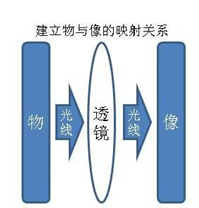
\includegraphics[width=0.3\textwidth]{fig6a.png}
    }
    \subfigure[阿贝成像原理光学图像]{
        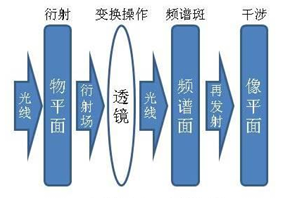
\includegraphics[width=0.3\textwidth]{fig6b.png}
    }
    \subfigure[基于波前的现代光学图像]{
        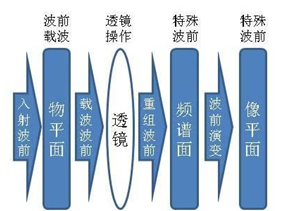
\includegraphics[width=0.3\textwidth]{fig6c.png}
    }
    \caption{透镜成像的不同理解与物理图像}
    \label{fig:imaging_models}
\end{figure}

阿贝成像原理在波动光学的衍射和干涉概念基础上，通过引入傅里叶变换的数学工具，建立了频谱面、频谱花样与物信息的关联，为空间滤波技术提供了理论支撑，成为傅里叶变换光学的基石。其核心价值在于揭示了透镜成像的傅里叶变换本质，明确了频谱面的存在及其重要性。

\subsubsection{阿贝成像原理的数学证明}
阿贝成像原理的证明思路可概括为以下步骤（参见图\ref{fig:abbe_principle}）：

	\textbf{0. 基本假设}：物、透镜、频谱面和像面均位于$xy$平面，光场沿$z$方向传播；透镜焦距为$F$，照明光源为单色相干光（波长$\lambda$）。

	\textbf{1. 物的波前表示}：
任意物对单色平行入射光的调制，可分解为一系列沿空间方向变化的余弦光栅叠加。仅考虑$x$方向时，物光波前可表示为：
\begin{equation}
U_o(x,y) = A_0 + \sum_{n} A_n \cos(2\pi f_n x + \phi_n)
\end{equation}
其中$f_n$为空间频率，$A_n$为振幅，$\phi_n$为相位。利用欧拉公式可改写为：
\begin{equation}
U_o(x,y) = A_0 + \sum_{n} \frac{A_n}{2} \left[ e^{i(2\pi f_n x + \phi_n)} + e^{-i(2\pi f_n x + \phi_n)} \right]
\end{equation}

	\textbf{2. 频谱面的形成}：
单频分量$A_n \cos(2\pi f_n x)$经物镜变换后，在频谱面（后焦面）形成三个衍射斑：
\begin{itemize}
    \item 中心斑$S_0$：对应0频分量，位置$x=0$；
    \item 正负一级斑$S_{\pm1}$：对称分布于$x$方向，满足
    \begin{equation}
    x_{\pm1} = \pm F \tan\theta_n \approx \pm F \sin\theta_n = \pm F \lambda f_n
    \end{equation}
    其中$\theta_n$为衍射角，满足光栅方程$\sin\theta_n = \lambda f_n$。
\end{itemize}

三个衍射斑的复振幅分别为：
\begin{align}
U(S_0) &\propto A_0 \\
U(S_{+1}) &\propto \frac{A_n}{2} e^{i\phi_n} \\
U(S_{-1}) &\propto \frac{A_n}{2} e^{-i\phi_n}
\end{align}

	\textbf{3. 像面的干涉重构}：
频谱面的三个相干光源发射球面波，在像面产生干涉。其复振幅分布为：
\begin{equation}
U_i(x',y') = A_0 + \sum_{n} A_n \cos\left(2\pi f_n \frac{x'}{V} + \phi_n\right)
\end{equation}
其中$V = \frac{x'}{x}$为放大率。

\begin{figure}[htbp]
    \centering
    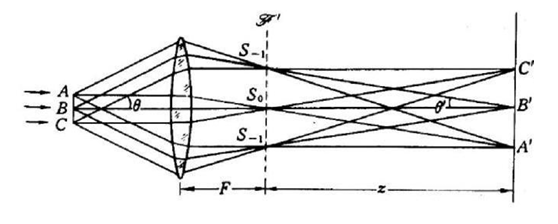
\includegraphics[width=0.8\textwidth]{fig7.png}
    \caption{阿贝成像原理说明图}
    \label{fig:abbe_principle}
\end{figure}

\subsubsection{分析}
通过上述分析可总结如下：
\begin{enumerate}
    \item 物的单一空间频率分量 $f_n$ 在像面上重构为频率 $f'_n = \dfrac{f_n}{V}$ 的相似信号，放大率 $V = \dfrac{f'_n}{f_n}$；
    \item 复杂物体可视为多频分量的叠加，像面为各分量的组合，整体放大率同为 $V$；
    \item 频谱面中心斑 $S_0$ 对应 0 频（直流分量），$\pm1$ 级斑对应 $\pm f_n$ 的频率分量。空间频率越高（$f_n$ 越大），衍射角 $\theta_n$ 越大，衍射斑距中心越远。
\end{enumerate}

后续实验将围绕光源准直、透镜成像、频谱面观测及频谱操作展开，以验证上述理论。

\subsection{光学4F图像}
单透镜成像系统虽结构简单，但在相干光学图像处理中存在显著局限。为克服这些不足，4F系统通过分离傅里叶变换与成像功能，成为相干光学处理的经典架构。

\subsubsection{单透镜成像系统的局限性}
单透镜系统的核心缺陷可从物理原理与实际应用两方面分析：
\begin{enumerate}
    \item \textbf{功能冲突性}：成像需求（如放大率调节）与频谱面处理需求存在固有矛盾。例如，若需通过缩小像尺寸提高亮度（减小像距），会导致物的衍射光超出透镜孔径，引发高频信息丢失（见图\ref{fig:4f_system}）。设透镜孔径为$D$，物距为$d_o$，物的最大空间频率为$f_{\text{max}}$，则衍射角满足$\sin\theta \approx \lambda f_{\text{max}}$，当$d_o \cdot \tan\theta > D/2$时，高频分量被截断，信息丢失量为：
    \begin{equation}
        \Delta f = f_{\text{max}} - \frac{D}{2\lambda d_o}
    \end{equation}
    \item \textbf{相位失真问题}：单透镜成像时，像场函数与物场函数存在额外相位因子。设物场为$g(x_0,y_0)$，经焦距为$f$的透镜成像后，像场$g'(x',y')$满足：
    \begin{equation}
        g'(x',y') = \mathcal{F}^{-1}\left\{ \mathcal{F}\{g(x_0,y_0)\} \cdot \exp\left(-i\frac{k(x_1^2 + y_1^2)}{2f}\right) \right\}
    \end{equation}
    其中$\mathcal{F}$表示傅里叶变换，$(x_1,y_1)$为频谱面坐标，$k=2\pi/\lambda$为波数。额外相位项$\exp\left(-i\frac{k(x_1^2 + y_1^2)}{2f}\right)$破坏了相位保真度，而相干光学中相位信息对干涉、全息等应用至关重要。
\end{enumerate}

\subsubsection{4F系统的结构与工作原理}
4F系统由两个共轴透镜（焦距均为$f$）构成，沿光轴依次为：物平面、透镜1（傅里叶变换透镜）、频谱面、透镜2（反傅里叶变换透镜）、像平面，各平面间距均为$f$，总光程为$4f$，故得名（见图\ref{fig:4f_system}）。

\begin{figure}[htbp]
    \centering
    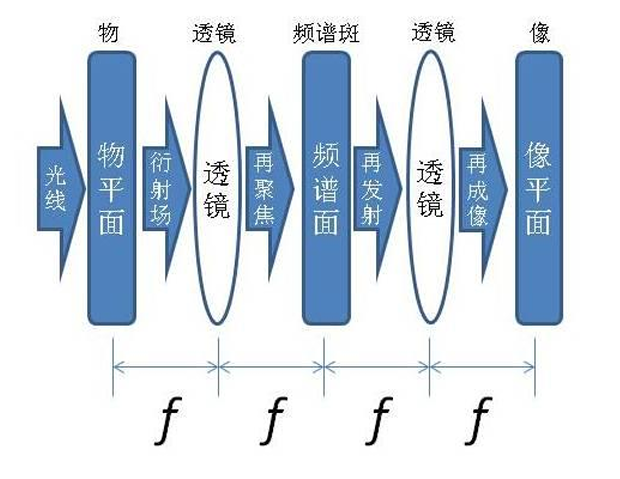
\includegraphics[width=0.8\textwidth]{fig10.png}
    \caption{4F相干光学处理系统结构示意图}
    \label{fig:4f_system}
\end{figure}

其工作机制基于两次傅里叶变换的级联：
\begin{enumerate}
    \item \textbf{第一次傅里叶变换（透镜1）}：物平面（透镜1前焦面）上的物场$g(x_0,y_0)$经透镜1衍射后，在其后焦面（频谱面）形成傅里叶变换谱：
    \begin{equation}
        G(f_x,f_y) = \mathcal{F}\{g(x_0,y_0)\} = \iint_{-\infty}^{\infty} g(x_0,y_0) \exp\left(-i2\pi(f_x x_0 + f_y y_0)\right) dx_0 dy_0
    \end{equation}
    其中空间频率与频谱面坐标的关系为$f_x = x_1/(\lambda f)$，$f_y = y_1/(\lambda f)$，$(x_1,y_1)$为频谱面坐标。
    \item \textbf{第二次傅里叶变换（透镜2）}：频谱面位于透镜2的前焦面，其场分布$G(x_1,y_1)$经透镜2变换后，在像平面（透镜2后焦面）形成反傅里叶变换：
    \begin{equation}
        g'(x,y) = \mathcal{F}^{-1}\{G(f_x,f_y)\} = \iint_{-\infty}^{\infty} G(f_x,f_y) \exp\left(i2\pi(f_x x + f_y y)\right) df_x df_y
    \end{equation}
    因两次变换引入坐标反转（$x = -x_0$，$y = -y_0$），像平面采用与物平面反向的坐标系，可抵消变换中的负号，最终像场为$g'(x,y) = g(-x,-y)$，实现相位保真。
\end{enumerate}

\subsubsection{4F系统的核心优势}
\begin{enumerate}
    \item \textbf{功能分离性}：傅里叶变换（透镜1）与成像（透镜2）功能独立。调节透镜2焦距可改变放大率$M = f_2/f_1$（$f_1,f_2$分别为两透镜焦距），且不影响透镜1的频谱变换效果，解决了单透镜的功能冲突。
    \item \textbf{相位保真度}：透镜1的相位因子$\exp\left(-i\frac{k(x_1^2 + y_1^2)}{2f}\right)$被透镜2的逆相位因子抵消，当$M=1$且无滤波时，像场严格复制物场的振幅与相位：
    \begin{equation}
        g'(x,y) = g(x,y) \quad (\text{忽略坐标反转的物理等效性})
    \end{equation}
    \item \textbf{灵活的频谱调控}：频谱面可插入空间滤波器（如高通、低通、方向滤波器），直接对$G(f_x,f_y)$进行调制，实现图像增强、噪声抑制等处理（见图\ref{fig:4f_imaging}）。
\end{enumerate}

\begin{figure}[htbp]
    \centering
    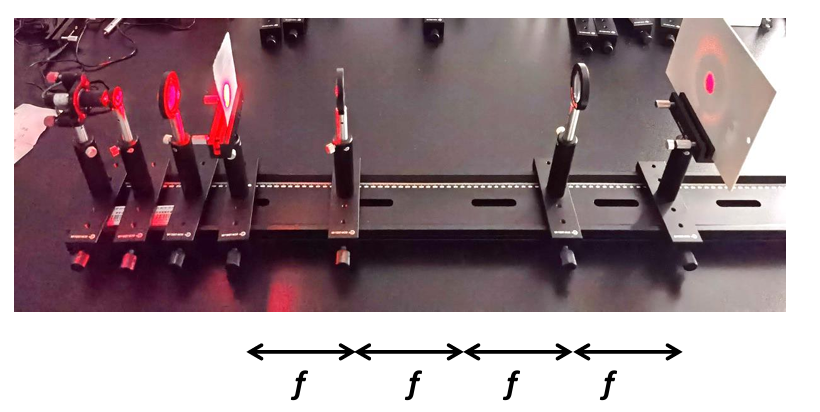
\includegraphics[width=0.7\textwidth]{fig11.png}
    \caption{4F系统成像与频谱调控过程}
    \label{fig:4f_imaging}
\end{figure}

综上，4F系统通过光学傅里叶变换的级联，在保持相位保真的同时实现了成像与频谱处理的解耦，成为相干光学信息处理的标准架构。

\subsection{θ调制空间假彩色编码实验原理与装置}
θ调制空间假彩色编码实验基于阿贝成像原理，通过对物面不同区域施加方向选择性光栅调制，并结合白光照明下的衍射色散，实现图像分区的人工彩色编码。该方法充分利用光栅的方向敏感性和波长依赖性，是空间滤波在彩色信息处理中的典型应用。

\subsubsection{θ调制原理与样品结构}
θ调制的核心在于：对物体不同区域分别施加不同取向的光栅调制。实验样品为天安门图案（见图\ref{fig:theta_modulation_sample}a），其天空、主体、草地三区域分别通过三次曝光记录不同方向的光栅，空间频率均为 $f=100\ \text{lines/mm}$。光栅常数 $d$ 与空间频率 $f$ 满足：
\begin{equation}
    f = \frac{1}{d} \implies d = 10\ \mu\text{m}
\end{equation}
不同区域的光栅取向差（$\theta$ 角）使各区域衍射光在空间上分离，为后续颜色编码提供物理基础（见图\ref{fig:theta_modulation_sample}b）。

\begin{figure}[htbp]
    \centering
    \subfigure[被调制物结构示意]{
        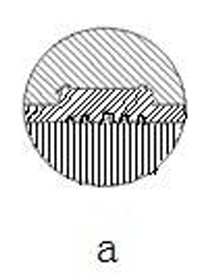
\includegraphics[width=0.25\textwidth]{fig12a.png}
    }
    \subfigure[分区衍射方向示意]{
        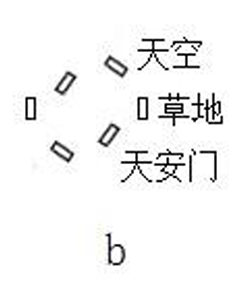
\includegraphics[width=0.25\textwidth]{fig12b.png}
    }
    \subfigure[目标分区着色效果]{
        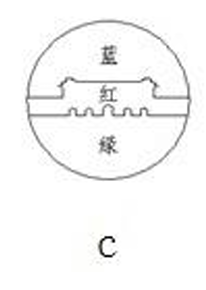
\includegraphics[width=0.25\textwidth]{fig12c.png}
    }
    \caption{θ调制样品结构与分区衍射、着色效果示意}
    \label{fig:theta_modulation_sample}
\end{figure}

\begin{figure}[htbp]
    \centering
    \begin{tikzpicture}[node distance=1cm,>=Stealth]
        \node (src) [draw, rectangle, minimum width=1.5cm, minimum height=0.8cm] {白光源};
        \node (coll) [draw, rectangle, right=of src, minimum width=1.5cm, minimum height=0.8cm] {准直镜};
        \node (obj) [draw, rectangle, right=of coll, minimum width=1.5cm, minimum height=0.8cm] {θ调制物};
        \node (ftlens) [draw, rectangle, right=of obj, minimum width=1.5cm, minimum height=0.8cm] {傅里叶透镜};
        \node (filter) [draw, rectangle, right=of ftlens, minimum width=1.5cm, minimum height=0.8cm] {空间滤波器};
        \node (imlens) [draw, rectangle, right=of filter, minimum width=1.5cm, minimum height=0.8cm] {成像透镜};
        \node (screen) [draw, rectangle, right=of imlens, minimum width=1.5cm, minimum height=0.8cm] {白屏/像面};
        \draw[->, thick] (src) -- (coll);
        \draw[->, thick] (coll) -- (obj);
        \draw[->, thick] (obj) -- (ftlens);
        \draw[->, thick] (ftlens) -- (filter);
        \draw[->, thick] (filter) -- (imlens);
        \draw[->, thick] (imlens) -- (screen);
    \end{tikzpicture}
    \caption{θ调制假彩色编码实验系统流程示意}
    \label{fig:theta_flow}
\end{figure}

\subsubsection{白光衍射与频谱面特性}
白光（400--760 nm）照射调制物后，各区域光栅满足多色光衍射。光栅方程：
\begin{equation}
    d\sin\theta_m = m\lambda, \quad m=0,\pm1,\pm2,\dots
\end{equation}
其中 $m$ 为衍射级次，$\theta_m$ 为 $m$ 级衍射角。对同一级次，$\theta_m$ 随 $\lambda$ 增大而增大，导致不同颜色光沿衍射方向分散，形成彩色谱带。

经傅里叶透镜作用，频谱面上出现与光栅方向对应的彩色频谱花样（见图\ref{fig:theta_filter}b）：
\begin{itemize}
    \item 0级谱：中心白光直射分量，无方向选择性；
    \item $\pm1$级谱：沿光栅取向的垂直方向展开，红（长波）在外、蓝（短波）在内。不同区域的光栅取向不同，其$\pm1$级谱带在频谱面方位角不同（与光栅方向垂直）。
\end{itemize}
方位角与波长的双重选择性，使频谱面成为颜色编码的关键调控面。

\subsubsection{空间选色滤波与假彩色成像}
假彩色编码通过在频谱面插入空间滤波器实现，对不同方位的彩色谱带进行选择性透射：
\begin{enumerate}
    \item \textbf{颜色滤光片法}：在频谱面对应区域（如天空光栅的$\pm1$级谱带）放置特定颜色滤光片（如蓝色），仅允许该颜色光通过；
    \item \textbf{自制空间滤波器}：在白纸或胶片上对应谱带位置开孔，仅让目标波长范围的光透过。
\end{enumerate}
经成像透镜二次傅里叶变换后，像面各区域的颜色由其对应频谱被允许通过的波长决定。实验目标为：草地区域透过绿光、天安门区域透过红光、天空区域透过蓝光（见图\ref{fig:theta_modulation_sample}c）。其物理本质为：
\begin{equation}
    C(x,y) = \sum_{\lambda \in \Lambda_{\theta(x,y)}} I(\lambda) \, t(\lambda,\theta(x,y))
\end{equation}
其中 $\Lambda_{\theta(x,y)}$ 为 $(x,y)$ 处光栅允许的衍射波长集合，$t(\lambda,\theta)$ 为滤波器在角度 $\theta$ 处对波长 $\lambda$ 的透射率，$I(\lambda)$ 为入射白光的光谱强度。

\begin{figure}[htbp]
    \centering
    \subfigure[空间滤波原理框图]{
        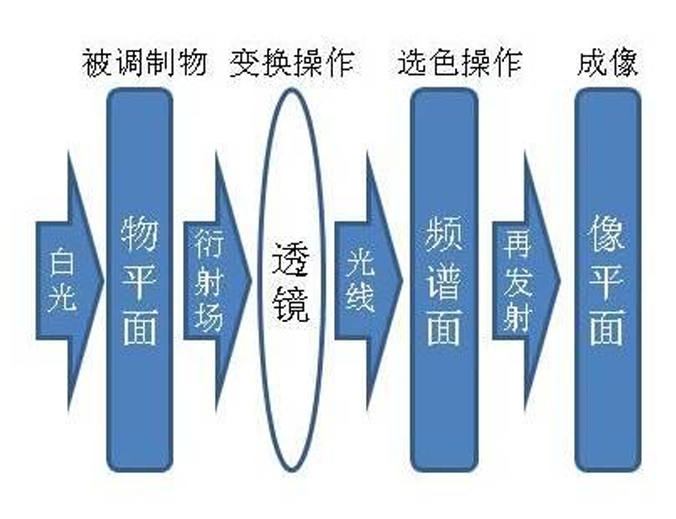
\includegraphics[width=0.5\textwidth]{fig13a.png}
    }
    \subfigure[θ调制频谱花样与选色示意]{
        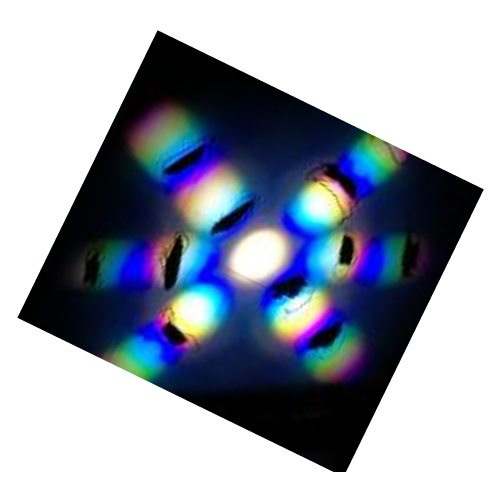
\includegraphics[width=0.3\textwidth]{fig13b.png}
    }
    \caption{θ调制空间滤波系统与频谱特性}
    \label{fig:theta_filter}
\end{figure}

\subsubsection{实验仪器与系统组成}
实验系统由六大核心组件构成，各自功能与参数如下表：
\begin{table}[htbp]
    \centering
    \renewcommand{\arraystretch}{1.2}
    \begin{tabular}{|c|l|}
        \hline
        	\textbf{组件名称} & \textbf{主要器件及参数} \\
        \hline
        光源组件 & 白光LED（400--760 nm）、一维平移台、宽滑块、支架、套筒 \\
        \hline
        准直镜组件 & 凸透镜（$\Phi40\ \text{mm}$，$f=80\ \text{mm}$）、透镜架、滑块、支架、套筒 \\
        \hline
        调制物组件 & 天安门光栅（$f=100\ \text{lines/mm}$，三区不同取向）、干板架、滑块、支架、套筒 \\
        \hline
        变换透镜组件 & 凸透镜（$\Phi76\ \text{mm}$，$f=175\ \text{mm}$）、镜架、滑块、支架、套筒 \\
        \hline
        滤波器组件 & 红/绿/蓝滤光片（半带宽$<50\ \text{nm}$）、自制空间滤波器、干板架、滑块、支架、套筒 \\
        \hline
        白屏组件 & 白屏（像面）、干板架、滑块、支架、套筒 \\
        \hline
    \end{tabular}
    \caption{θ调制假彩色编码实验仪器系统组成}
    \label{tab:theta_instruments}
\end{table}

系统光路严格满足4F架构：光源经准直镜形成平行白光，照射调制物后经傅里叶透镜（前焦面为物面）在其后焦面形成频谱（滤波面），再经成像透镜（与傅里叶透镜共焦）在像面生成编码彩色图像，总光程匹配透镜焦距以保证傅里叶变换的准确性。

\section{实验操作}

\subsection{薄透镜焦距的测定}

\subsubsection{成像公式法测定凸透镜焦距}
\begin{enumerate}
    \item 搭建光学平台：将凸透镜固定在光具座上，物屏（十字叉丝或箭头）置于透镜左侧，像屏（毛玻璃或白纸）置于右侧。
    \item 调节物距：移动物屏，使其距离透镜大于2倍焦距（约50--100 cm），观察像屏上的倒立缩小实像。
    \item 测量距离：使用米尺测量物距$s$（物屏到透镜光心的距离）和像距$s'$（透镜光心到像屏的距离）。
    \item 计算焦距：根据公式$f = \frac{ss'}{s + s'}$计算焦距。重复测量3--5次，取平均值。
    \item 验证成像规律：改变物距，观察像的倒正、放大缩小特性，记录数据并绘制成像规律表。
\end{enumerate}

\subsubsection{二次成像法测定凸透镜焦距}
\begin{enumerate}
    \item 固定物屏和像屏：将物屏和像屏固定在光具座上，间距$D > 4f$（约1--1.5 m）。
    \item 移动透镜：将凸透镜置于物屏和像屏之间，移动透镜找到两个位置，使像屏上形成清晰实像。
    \item 记录位置：测量两个成像位置的透镜位移$d$。
    \item 计算焦距：根据公式$f = \frac{D^2 - d^2}{4D}$计算焦距。重复测量以减小误差。
\end{enumerate}

\subsubsection{自准直法测定凸透镜焦距}
\begin{enumerate}
    \item 搭建系统：将凸透镜固定，左侧置物屏$AB$（十字叉丝），右侧置平面镜$M$垂直于光轴。
    \item 调节位置：移动物屏，使其位于透镜焦平面附近，观察镜面反射光经透镜后在原物屏形成等大倒立实像。
    \item 测量焦距：此时物屏到透镜的距离即为焦距$f$。精确调节位置以获得最清晰像。
\end{enumerate}

\subsubsection{辅助透镜法测定凹透镜焦距}
\begin{enumerate}
    \item 搭建系统：使用凸透镜$L_1$（焦距已知）使物$AB$成实像$A'B'$。
    \item 插入凹透镜：在$L_1$与$A'B'$之间插入凹透镜$L_2$，调节位置使$A'B'$作为$L_2$的虚物，成实像$A''B''$。
    \item 测量距离：测$L_2$到$A'B'$的距离$s_2$（虚物，$s_2 < 0$）和到$A''B''$的距离$s_2'$（实像，$s_2' > 0$）。
    \item 计算焦距：根据公式$f_2' = \frac{s_2 s_2'}{s_2 + s_2'}$计算凹透镜焦距。
\end{enumerate}

\subsection{阿贝成像原理及空间滤波实验}

本实验旨在通过构建4F光学系统，验证阿贝成像原理，并利用空间滤波技术对图像频谱进行操作，观察其对成像质量及特征的影响。

\subsubsection{光路搭建与共轴调节}
\begin{enumerate}
    \item \textbf{光路布置}：参照图\ref{fig:4f_system}所示的4F系统结构，在光具座上自左向右依次安装：激光器组件、扩束镜组件、准直镜组件、光栅字组件（作为物）、变换透镜组件、滤波器组件和白屏组件（作为像面）。
    \item \textbf{组件间距参考}：为保证光路合理，建议相邻组件间距设置为：激光器与扩束镜间约40mm，扩束镜与准直镜间约70mm，准直镜与光栅字间约40mm，光栅字与变换透镜间约240mm，变换透镜与滤波器间约195mm，滤波器与白屏间约445mm。
    \item \textbf{等高共轴调节}：
    \begin{itemize}
        \item \textbf{激光器调节}：调整激光器高度（约90mm）及俯仰角，确保激光束沿导轨中心轴线水平传播。可通过在近处和远处分别测量白屏上的光斑高度来验证。
        \item \textbf{扩束与准直}：安装扩束镜，调节其支杆高度使光斑中心位于光轴上。接着安装准直镜，调节其位置（距扩束镜焦点处）以获得准直平行光束。
        \item \textbf{物与透镜安装}：安装光栅字（“光”字），调节高度使光束正入射。安装变换透镜，确保光束经过透镜中心。
    \end{itemize}
\end{enumerate}

\subsubsection{频谱观察与成像校准}
\begin{enumerate}
    \item \textbf{成像调节}：移动变换透镜位置，直至在白屏上观察到清晰放大的“光”字倒立实像，固定变换透镜。
    \item \textbf{频谱面定位}：安装滤波器支架，沿光轴前后移动，观察支架平面上的光斑分布。当观察到清晰锐利的衍射斑点阵（频谱）时，该位置即为频谱面（变换透镜后焦面），固定滤波器支架。
    \item \textbf{频谱特征观察}：在未加滤波器时，观察“光”字的频谱。由于实验所用“光”字由正交光栅（空间频率12线/mm）调制，其频谱呈现为二维正交点阵结构。
\end{enumerate}

\subsubsection{空间滤波操作与现象观察}
\begin{enumerate}
    \item \textbf{方向滤波（低通滤波）}：
    \begin{itemize}
        \item \textbf{保留竖直条纹}：将单缝滤波器置于频谱面，呈水平方向放置，调节缝宽与位置，使包括0级（中心亮斑）在内的一排水平频谱点通过。观察白屏像面，图像中应充满竖向条纹（横向高频信息丢失，保留横向直流及竖向基频）。
        \item \textbf{保留横向条纹}：旋转单缝滤波器90度，呈竖直方向放置，使包括0级在内的一排竖直频谱点通过。观察白屏像面，图像中应充满横向条纹。
        \item \textbf{45度方向滤波}：将单缝旋转至45度方向，观察像面条纹的变化情况。
    \end{itemize}
    \item \textbf{高通滤波（边缘提取）}：
    \begin{itemize}
        \item 将带有中心遮光点（或小孔滤波器反用）的滤波器置于频谱面，精确调节位置以阻挡0级频谱点（直流分量），同时允许高级次频谱通过。
        \item 观察白屏像面，此时图像背景变暗，明亮的实心字变为仅剩轮廓的空心字，实现了图像的边缘提取。
    \end{itemize}
\end{enumerate}

\subsection{光学4F系统成像实验}

本实验在阿贝成像实验的基础上，进一步构建完整的4F光学系统。该系统由两个焦距相同的透镜组成，通过两次傅里叶变换实现图像的1:1传输，是进行光学信息处理的标准架构。

\subsubsection{实验装置搭建与调节}
\begin{enumerate}
    \item \textbf{基础光路保留}：保持前序实验中的激光器、扩束镜、准直镜及白屏组件位置不变，确保系统照明光源为准直扩束后的平行光。
    \item \textbf{物平面（物孔）安装}：
    \begin{itemize}
        \item 将实验提供的物孔（光栅字或带字白纸）垂直安装于支架上。
        \item 调节支杆高度，使准直后的光斑中心正入射至物孔中心，确保物孔处于光场中心位置。
        \item 沿导轨移动物孔支架，使其尽可能靠近准直镜，以减少不必要的光程，调节完毕后锁紧滑块。
    \end{itemize}
    \item \textbf{第一傅里叶变换透镜（变换透镜1）安装}：
    \begin{itemize}
        \item 在物孔后方安装变换透镜1（焦距 $f=150\ \text{mm}$）。
        \item \textbf{共轴调节}：上下调整支杆，使透过物孔的光束准确穿过透镜中心（固定垂直高度）。
        \item \textbf{位置固定}：移动透镜1使其尽可能接近物孔（注意：此布局下物场紧贴透镜），并在此处固定透镜1的水平位置。
    \end{itemize}
    \item \textbf{第二傅里叶变换透镜（变换透镜2）安装}：
    \begin{itemize}
        \item 在变换透镜1后方安装变换透镜2（焦距 $f=150\ \text{mm}$）。
        \item \textbf{共轴调节}：同样调整高度，使光束穿过透镜2的中心。
        \item \textbf{间距调节}：移动透镜2，使其与透镜1的间距严格等于两倍焦距（$2f = 300\ \text{mm}$），并锁定位置。此时两透镜中间位置即为频谱面（共焦面）。
        \item \textbf{透镜朝向原则}：为减小像差，透镜放置应遵循“凹凸面对准平行光”的原则。同时注意透镜加工的非对称性，建议两个变换透镜对称或对易使用，确保焦距方向匹配。
    \end{itemize}
\end{enumerate}

\subsubsection{成像观察与频谱分析}
\begin{enumerate}
    \item \textbf{像面观察}：在白屏上观察成像特点。在4F系统中，应能观察到与物体等大、清晰的倒立实像。对比阿贝成像实验中的单透镜成像，分析两者在成像质量与性质上的区别。
    \item \textbf{频谱面实验}：在两透镜中间的频谱面（距透镜1和透镜2各 $f$ 处）安装滤波器支架。在此处放置不同的空间滤波器，观察像面图像的变化，验证傅里叶光学中的频域滤波原理。
\end{enumerate}

\subsection{θ调制空间假彩色编码实验操作}

本实验利用白光光源和θ调制板，通过在频谱面进行空间滤波（颜色编码），实现黑白图像的假彩色显示。

\subsubsection{光路布置和调节}
\begin{enumerate}
    \item \textbf{光路搭建}：参照图\ref{fig:theta_flow}布置光路，自左向右依次为：光源组件（白光LED）、准直镜组件、调制物组件（天安门光栅）、变换透镜组件、滤波器组件和白屏组件。
    \item \textbf{组件间距参考}：相邻组件水平方向间隔距离参考数值依次为：光源与准直镜约80mm，准直镜与调制物约40mm，调制物与变换透镜约275mm，变换透镜与滤波器约160mm，滤波器与白屏约335mm。
    \item \textbf{安装白光光源}：安装调整白光LED光源，调节支杆高度并固定于支杆靠近中间的位置，使得LED光源到支杆顶端的距离约为90mm（仅供参考）。
    \item \textbf{安装白屏}：将白屏固定在导轨右侧，尽量远一些。
    \item \textbf{安装准直镜}：
    \begin{itemize}
        \item 在距离LED发光点大约150mm附近放置准直透镜。
        \item 首先调节准直透镜的高度，使得LED光源发光点与准直透镜的中心水平对齐，并在白屏中心，固定准直透镜的垂直高度。
        \item 水平调节准直透镜的位置，直到通过其后的白光成为在近处和远处的光斑大小大致一样的准直光。
        \item \textbf{注意}：由于此处为白光光源，单透镜有色差，不可能作到绝对的准直；只要在远处的情况下，最中心的白色亮斑与近处时的白色亮斑大小一致即可。在此准直条件下，固定准直镜支撑滑块（即固定水平位置）。
    \end{itemize}
    \item \textbf{安装天安门光栅}：上下调整支杆使光斑正入射天安门中心，然后将其固定。
    \item \textbf{安装变换透镜}：上下调整支杆使入射光尽可能从变换透镜中心通过，此时在白屏上可看到模糊像，前后移动变换透镜直至在白屏上看到放大倒立实像，然后固定。
    \item \textbf{安装滤波器}：
    \begin{itemize}
        \item 安装滤波器支架，并安装一个纸片或者铁片于支架上。
        \item 沿导轨水平移动滤波器支架，并观察衍射光斑的变化：直到纸片或者铁片上呈现清晰的频谱面花样时（请参考图\ref{fig:theta_filter}，即为变换透镜的频谱面位置），在此处固定滤波器支架的水平位置。
        \item 后面，使用不同的滤波器于支架上，即可实现滤波。
    \end{itemize}
\end{enumerate}

\subsubsection{θ调制及现象观察}
\begin{enumerate}
    \item \textbf{使用θ调制滤波器}：根据预想的各部分图案所需要的颜色，使用提供的θ调制滤波器（三色滤片滤波器）实现指定的分区着色——蓝天、红色天安门、绿地。
    \begin{itemize}
        \item 首先，安装θ调制滤波器到滤波器支架上。
        \item 然后，调整θ调制滤波器的正反上下左右位置，使得调制器上的三色滤片与频谱面花样的指定分支相匹配。
        \item \textbf{匹配要求}：频谱面花样中的三个衍射方向上，应当让天安门图案对应的一组衍射频谱匹配红色的滤片（即让红色通过），草地对应的一组衍射频谱条匹配绿色的滤片（即让绿色通过），天空对应的一组衍射频谱条匹配蓝色的滤片（即让蓝色通过）。
        \item 调整好后，在后面白屏上观看经编码得到的假彩色像。
    \end{itemize}
    \item \textbf{使用自制滤波器}：
    \begin{itemize}
        \item 在实验过程中，可以使用提供的θ调制滤波器，也可以在实验室中找一张硬纸片，将硬纸片放在频谱面上并分别标记三个方向需要滤波通过的颜色。
        \item 然后在标记点扎孔并挖去要通过的部分（参考图\ref{fig:theta_filter}b），重新放回频谱面，即可观察滤波效果。
        \item 如果白光光源是LED光源，其光谱中的绿光成分可能会很弱，不易提取；可酌情考虑提取黄色来代替绿色。
    \end{itemize}
    \item \textbf{思考与观察}：
    \begin{itemize}
        \item 假彩色编码实验中使用的天安门城楼光栅本身中的城楼的窗户和门洞都是透光的，但是为什么经过所提供的假着色滤波处理后所成的像中这些窗户和门洞是黑色的？有方法验证你的解释吗？
        \item 扩展光源和点光源对比θ调制实验，观察哪一种情况天安门成像效果更佳。
    \end{itemize}
\end{enumerate}

\subsection{夫琅和费衍射与菲涅尔衍射演示实验}

本实验旨在通过观察不同结构分划板的衍射图样，验证夫琅和费衍射与菲涅尔衍射的基本理论，并理解巴比涅原理。

\subsubsection{实验内容与观察重点}
将分划板放入光路中（通常置于变换透镜前或直接在光路中观察），观察衍射图样的变化，并根据所学光学理论判断衍射图样与分划板参数的一致性。重点观察以下对比现象：
\begin{enumerate}
    \item \textbf{缝与孔}：对比单缝衍射与圆孔衍射（艾里斑）的图样区别。
    \item \textbf{互补屏}：对比缝与丝、圆孔与圆屏（障碍物）的衍射图样，验证巴比涅原理（Babinet's Principle）。
    \item \textbf{多缝干涉}：对比单缝、双缝与多缝衍射图样的区别，观察缺级现象及主极大、次极大的分布。
    \item \textbf{光栅维度}：对比一维光栅和二维光栅（网格）的衍射图样区别。
\end{enumerate}

\subsubsection{分划板参数说明}

实验所用分划板包含多种衍射单元，其具体参数如下：

\paragraph{分划板 1} 

\begin{figure}[htbp]
    \centering
    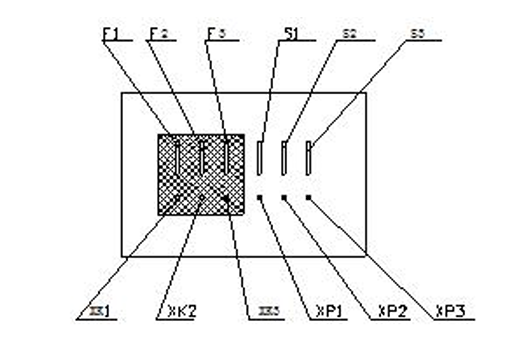
\includegraphics[width=0.8\textwidth]{fig14.png}
    \caption{分划板1}
\end{figure}

包含单缝、单丝、小孔及小屏，参数见表\ref{tab:reticle1}。

\begin{table}[H]
\centering
\caption{分划板1参数表（单位：mm）}
\label{tab:reticle1}
\begin{tabular}{|c|c|c|c|}
\hline
\textbf{类型} & \textbf{编号} & \textbf{参数说明} & \textbf{数值} \\
\hline
\multirow{3}{*}{单缝} & F1 & \multirow{3}{*}{缝宽 $a$} & 0.1 \\ \cline{2-2} \cline{4-4}
 & F2 & & 0.2 \\ \cline{2-2} \cline{4-4}
 & F3 & & 0.3 \\
\hline
\multirow{3}{*}{单丝} & S1 & \multirow{3}{*}{丝径 $a$} & 0.1 \\ \cline{2-2} \cline{4-4}
 & S2 & & 0.2 \\ \cline{2-2} \cline{4-4}
 & S3 & & 0.3 \\
\hline
\multirow{3}{*}{小孔} & XK1 & \multirow{3}{*}{孔径 $\phi$} & 0.2 \\ \cline{2-2} \cline{4-4}
 & XK2 & & 0.3 \\ \cline{2-2} \cline{4-4}
 & XK3 & & 0.4 \\
\hline
\multirow{3}{*}{小屏} & XP1 & \multirow{3}{*}{屏径 $\phi$} & 0.2 \\ \cline{2-2} \cline{4-4}
 & XP2 & & 0.3 \\ \cline{2-2} \cline{4-4}
 & XP3 & & 0.4 \\
\hline
\end{tabular}
\end{table}

\paragraph{分划板 2} 包含光栅、双孔、矩孔及多缝结构，参数见表\ref{tab:reticle2}。
\begin{figure}[htbp]
    \centering
    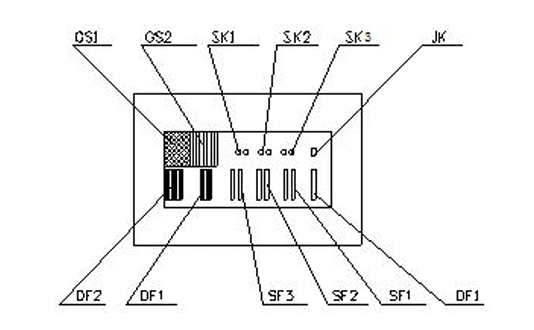
\includegraphics[width=0.8\textwidth]{fig15.png}
    \caption{分划板2}
\end{figure}
\begin{table}[H]
\centering
\caption{分划板2参数表（单位：mm）}
\label{tab:reticle2}
\begin{tabular}{|c|c|l|}
\hline
\textbf{类型} & \textbf{编号} & \textbf{参数说明} \\
\hline
\multirow{2}{*}{光栅} & GS1 & 纵横均为 50条/mm \\ \cline{2-3}
 & GS2 & 纵向 50条/mm \\
\hline
\multirow{3}{*}{双孔 ($\phi=0.2$)} & SK1 & 间距 $d=0.25$ \\ \cline{2-3}
 & SK2 & 间距 $d=0.32$ \\ \cline{2-3}
 & SK3 & 间距 $d=0.40$ \\
\hline
矩孔 & JK & 长宽 $a=0.12, b=0.2$ \\
\hline
单缝 & DF1 & 缝宽 $a=0.08$ \\
\hline
\multirow{3}{*}{双缝} & SF1 & $a=0.08, d=0.16$ \\ \cline{2-3}
 & SF2 & $a=0.08, d=0.20$ \\ \cline{2-3}
 & SF3 & $a=0.06, d=0.10$ \\
\hline
\multirow{2}{*}{多缝} & DF1 & 4缝, $a=0.06, d=0.1$ \\ \cline{2-3}
 & DF2 & 9缝, $a=0.06, d=0.1$ \\
\hline
\end{tabular}
\end{table}

\section{实验结果}
\subsection{阿贝尔成像实验图}
\begin{figure}[htbp]
    \centering
    \subfigure[光路图示]{
        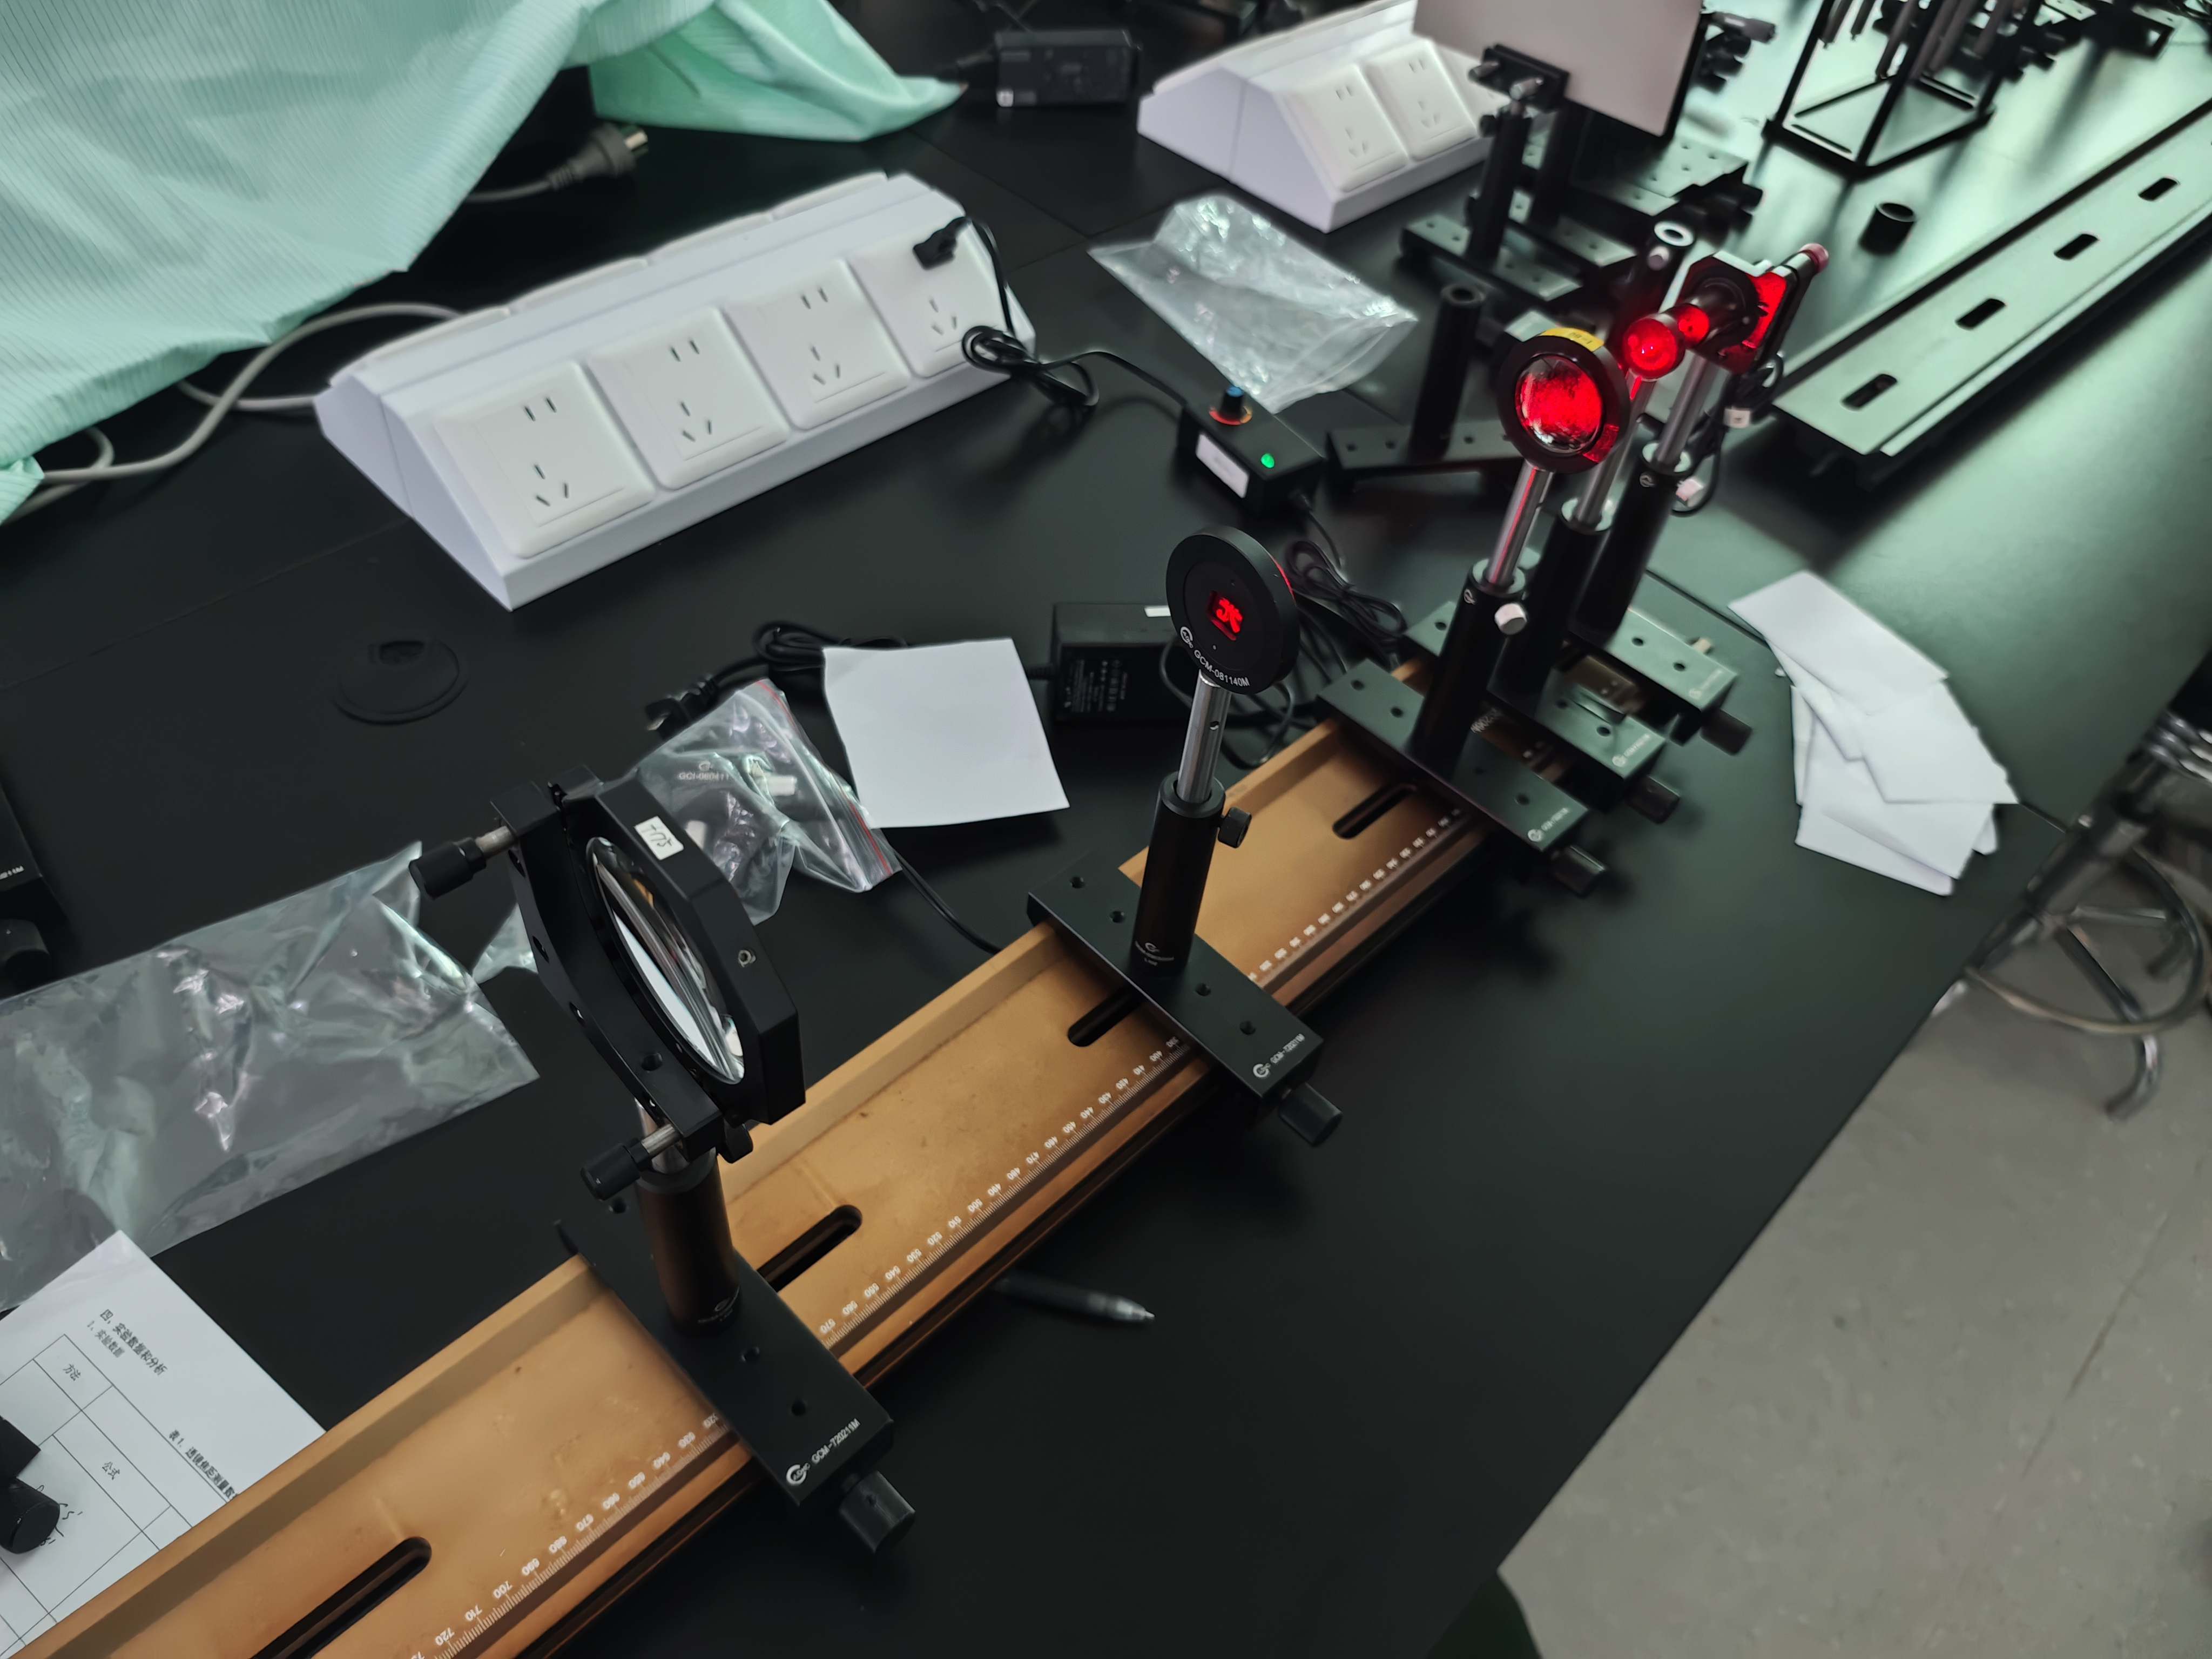
\includegraphics[width=0.4\textwidth]{fig 16a.jpg}
    }
    \vspace{0.5cm}
    \subfigure[成像]{
        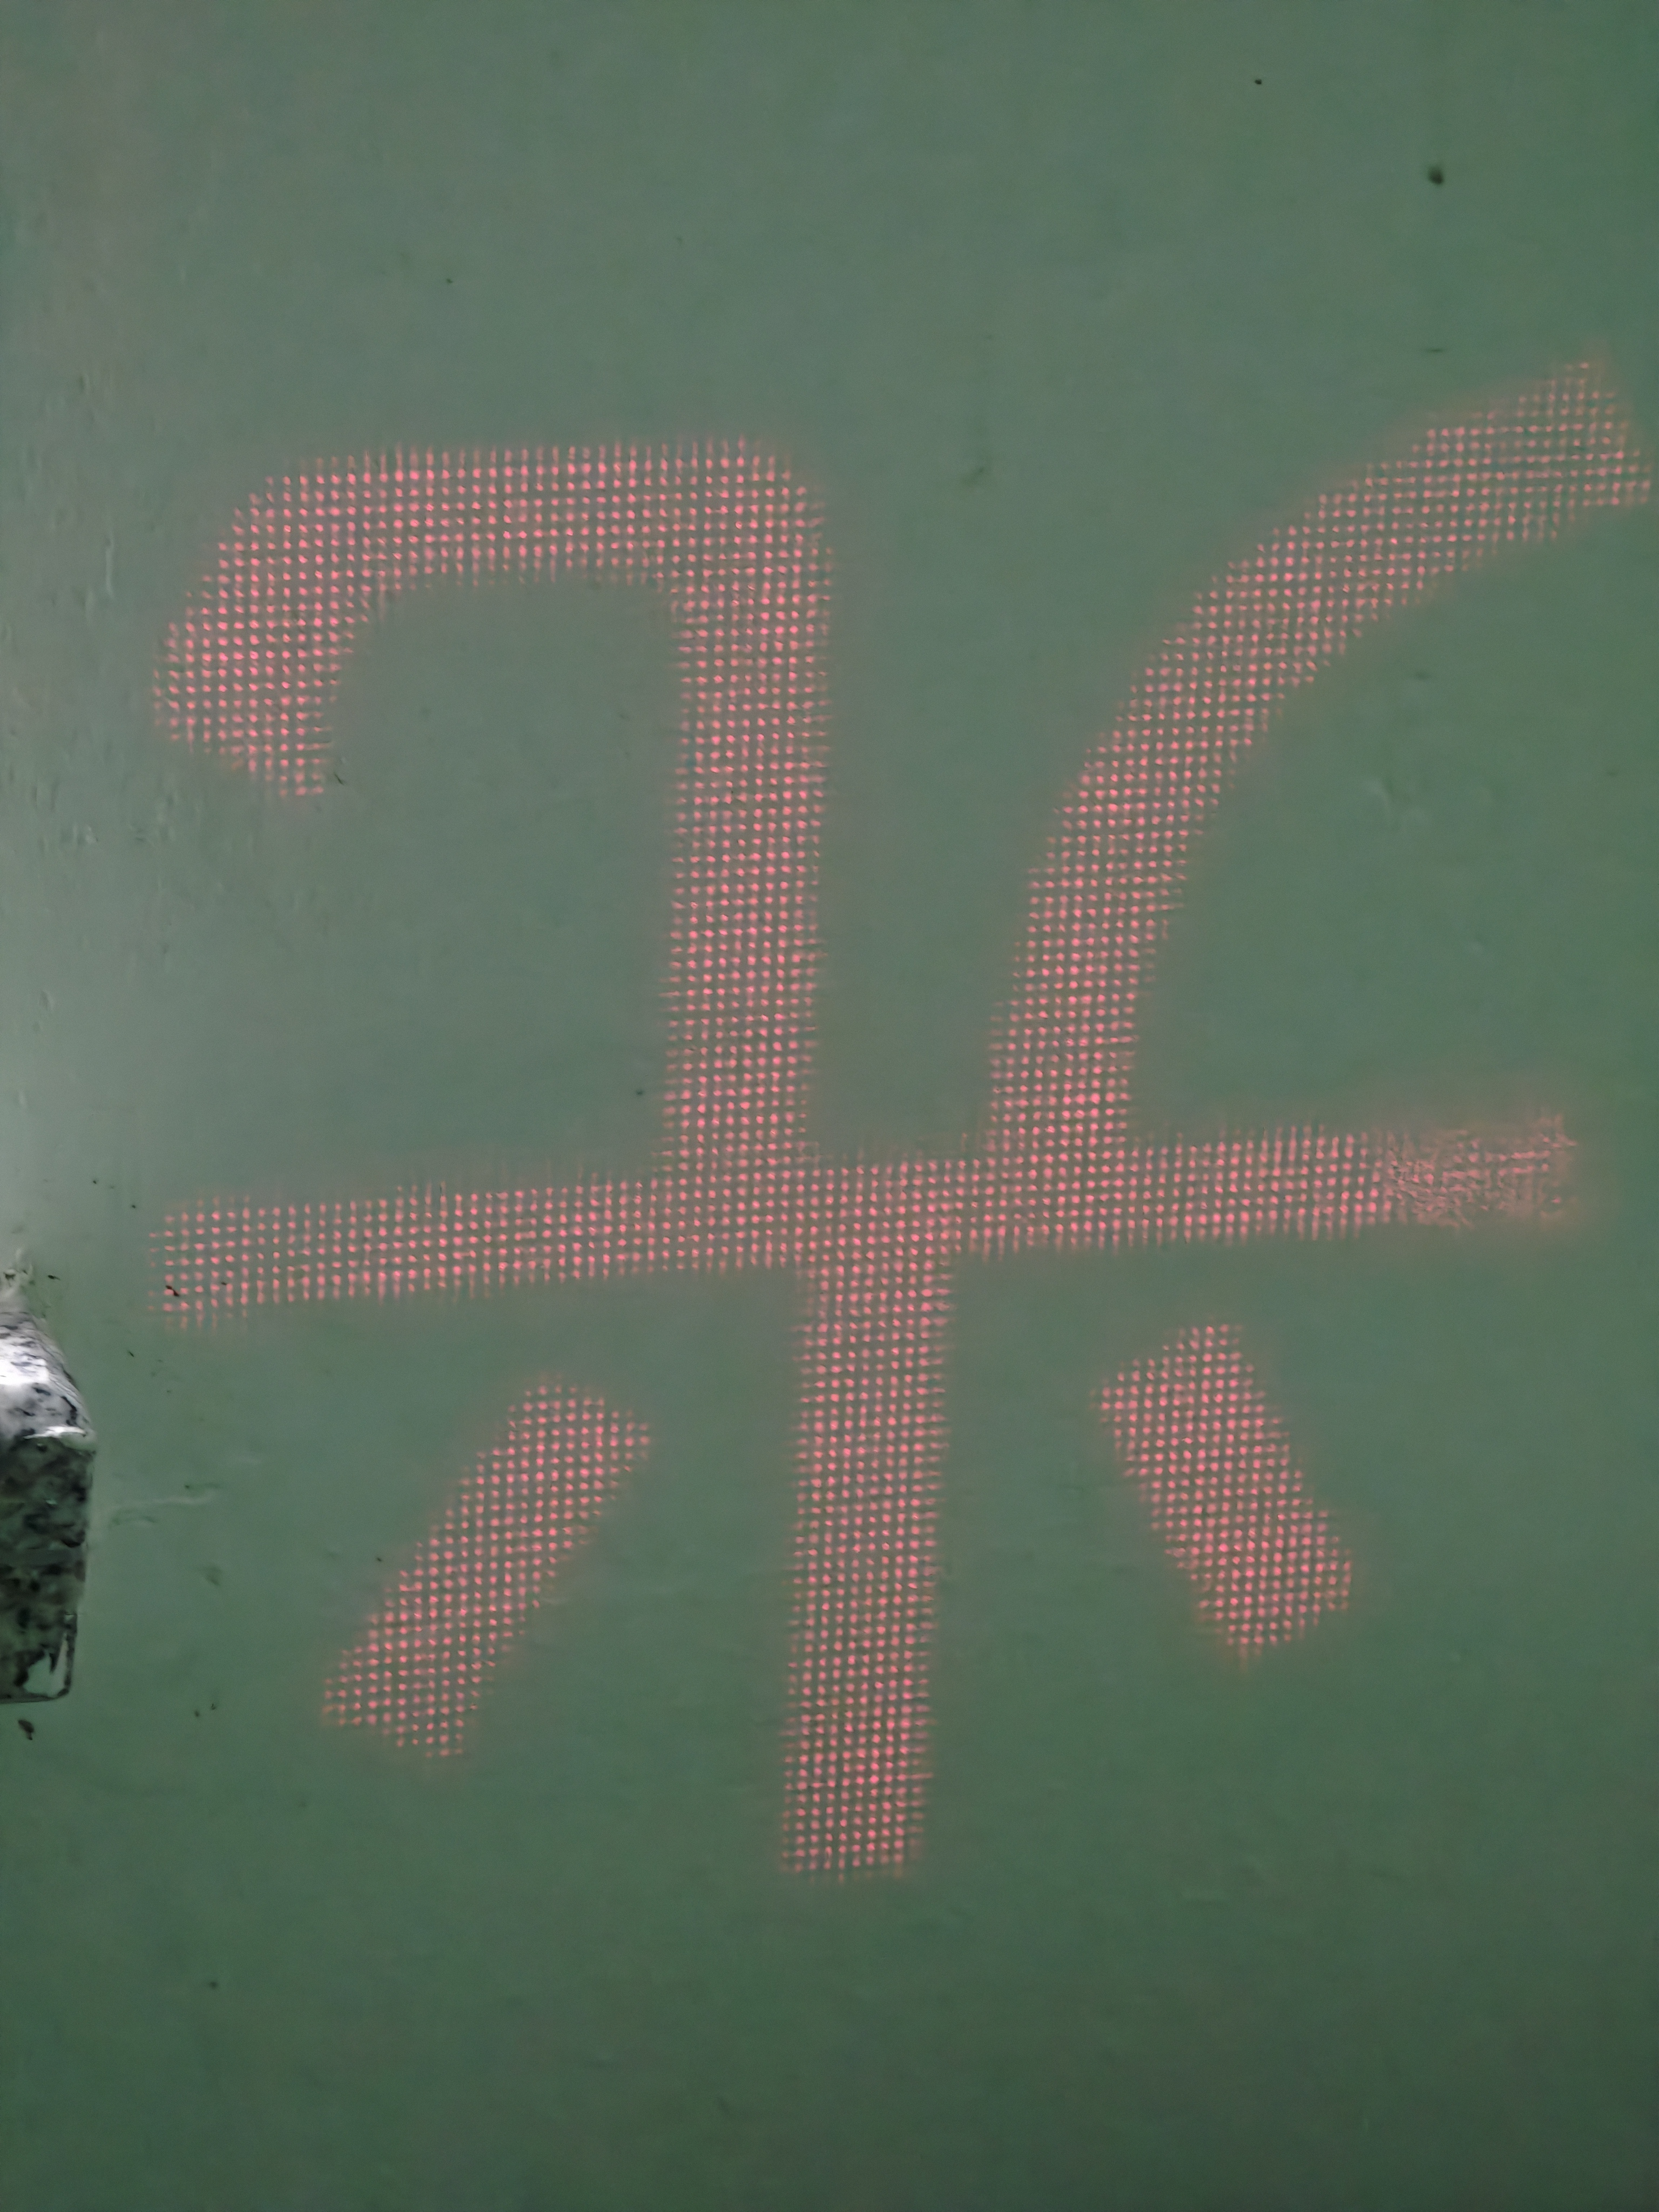
\includegraphics[width=0.4\textwidth]{fig 16b.jpg}
    }
    \caption{阿贝尔成像实验图1}
\end{figure}
\paragraph{透过光栅的成像}透过光栅时，像面显示出清晰的“光”字倒立实像，验证了阿贝成像原理。频谱面上呈现出二维正交点阵结构，符合光栅衍射特性。
\begin{figure}[htbp]
    \centering
    \subfigure[光路图示]{
        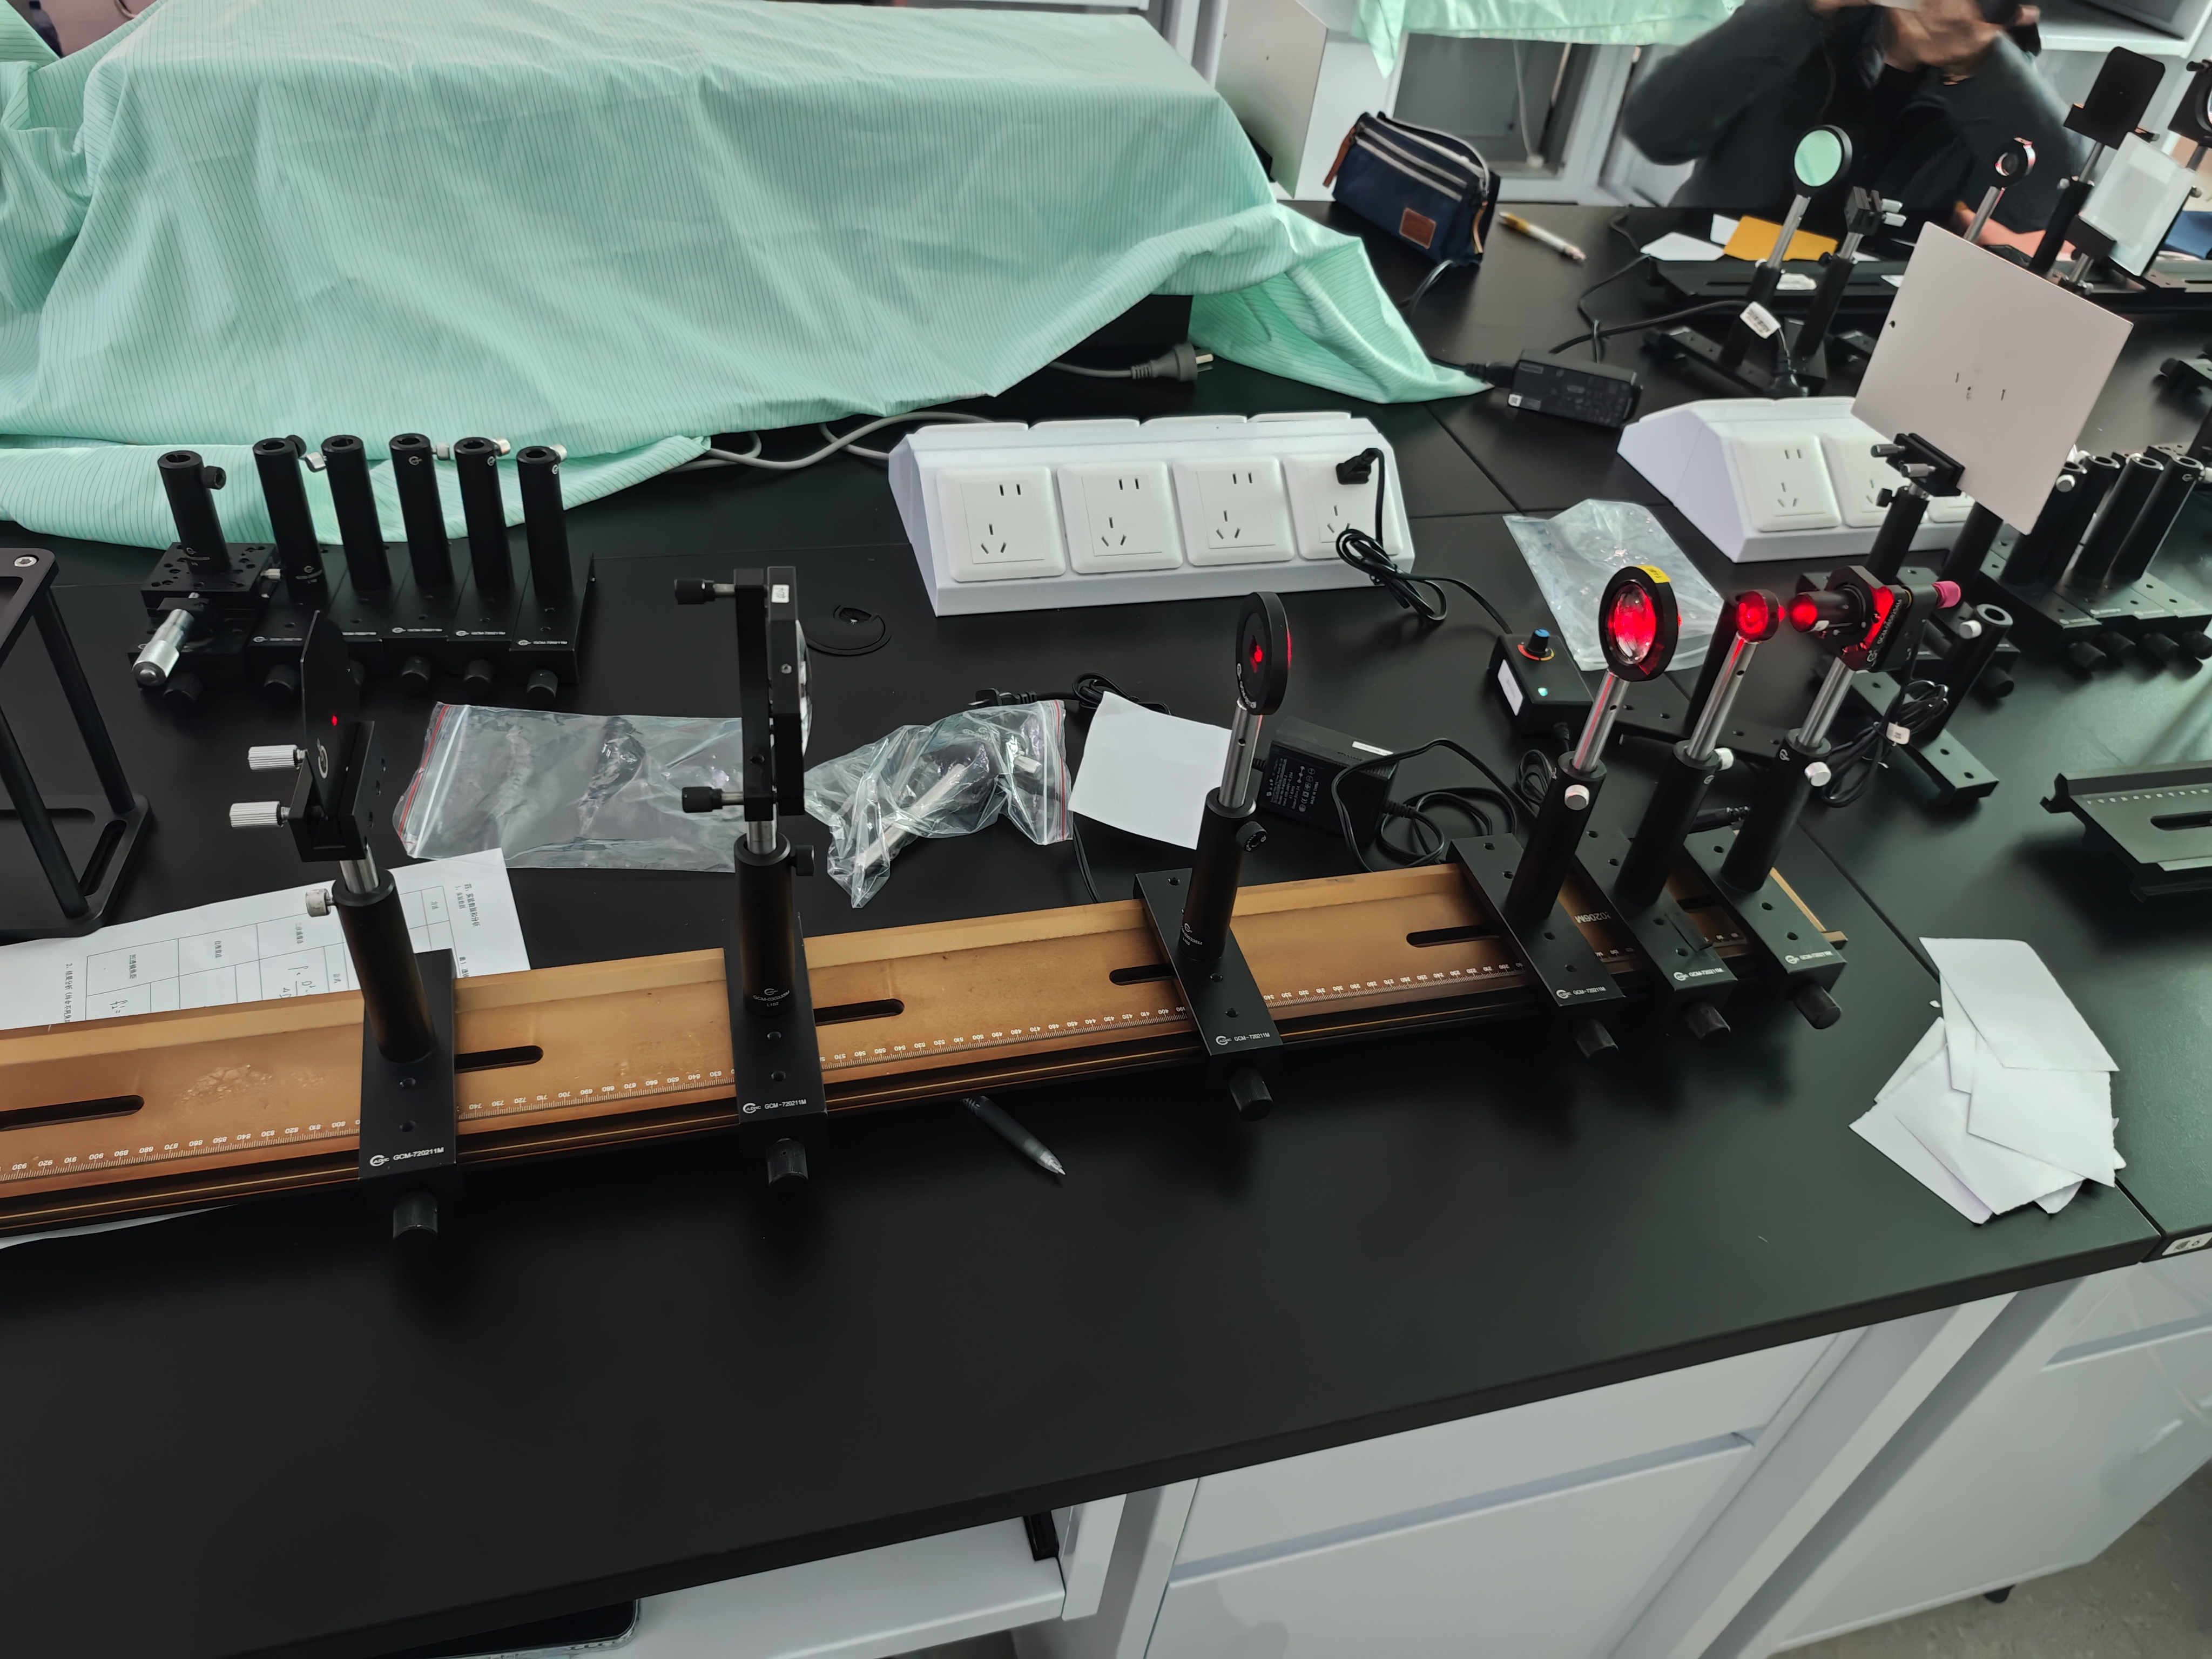
\includegraphics[width=0.25\textwidth]{fig17b.jpg}
    }
    \subfigure[成像]{
        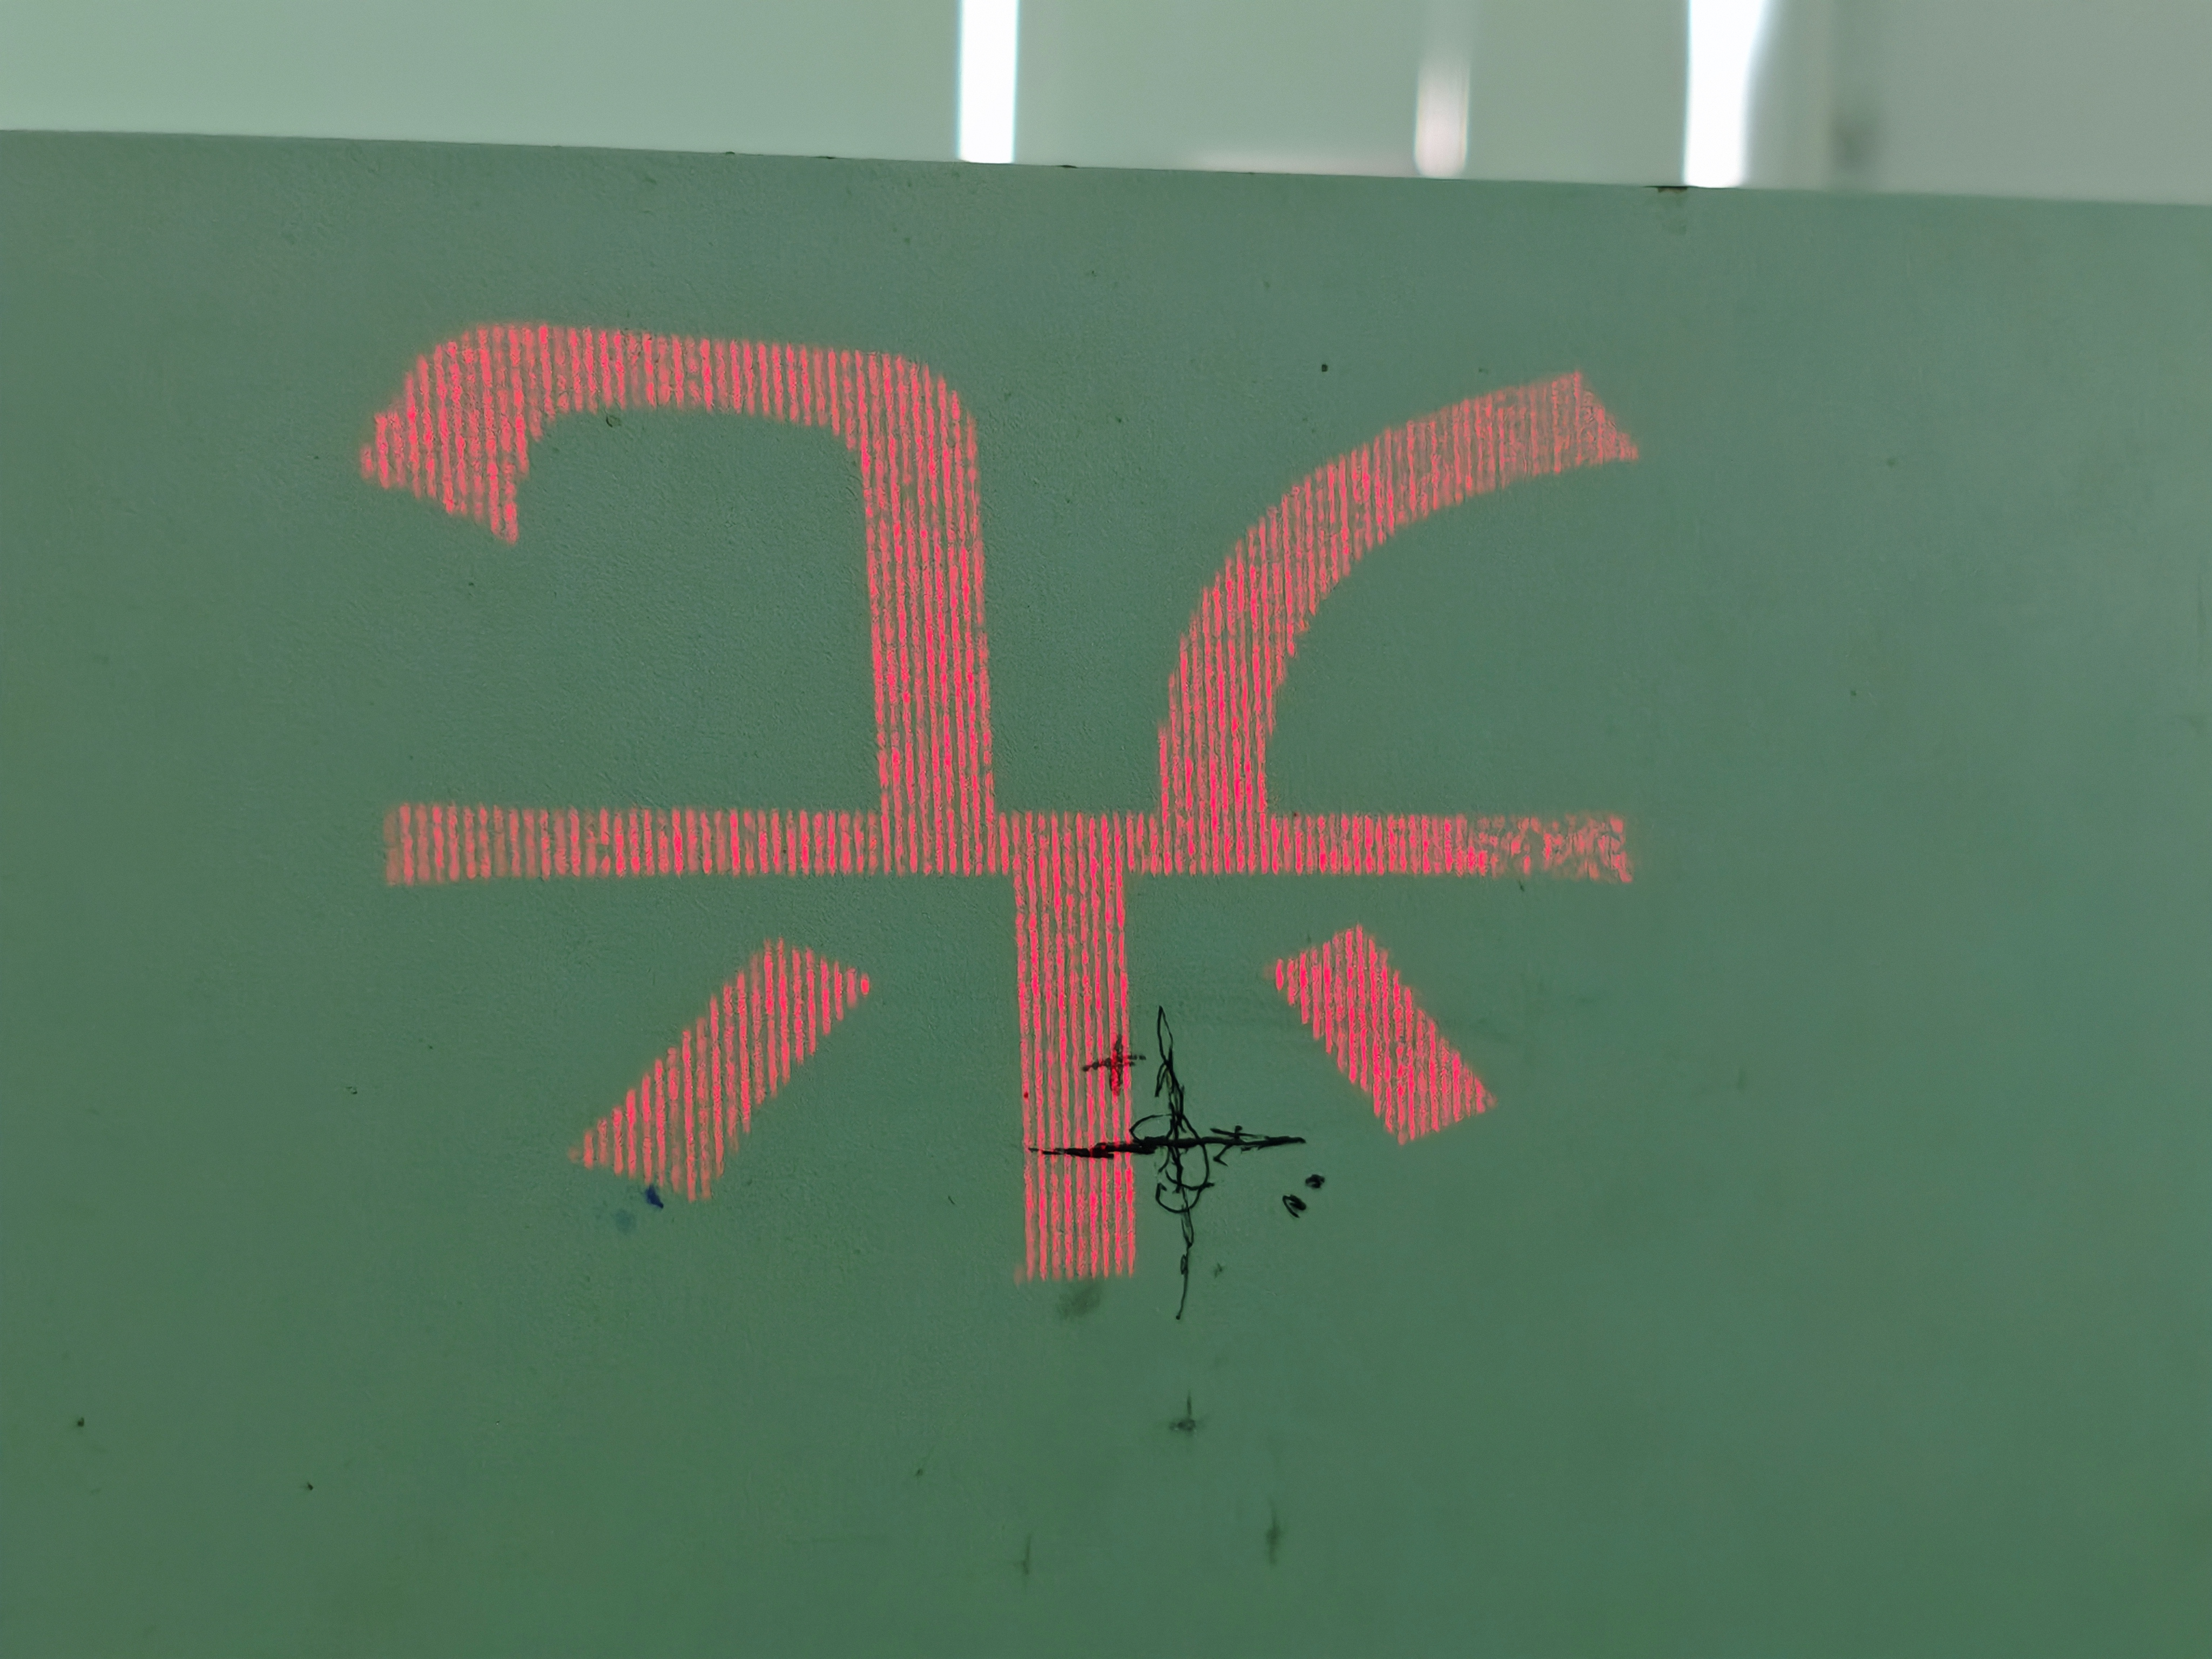
\includegraphics[width=0.25\textwidth]{fig17a.jpg}
    }
    \subfigure[频谱面图像]{
        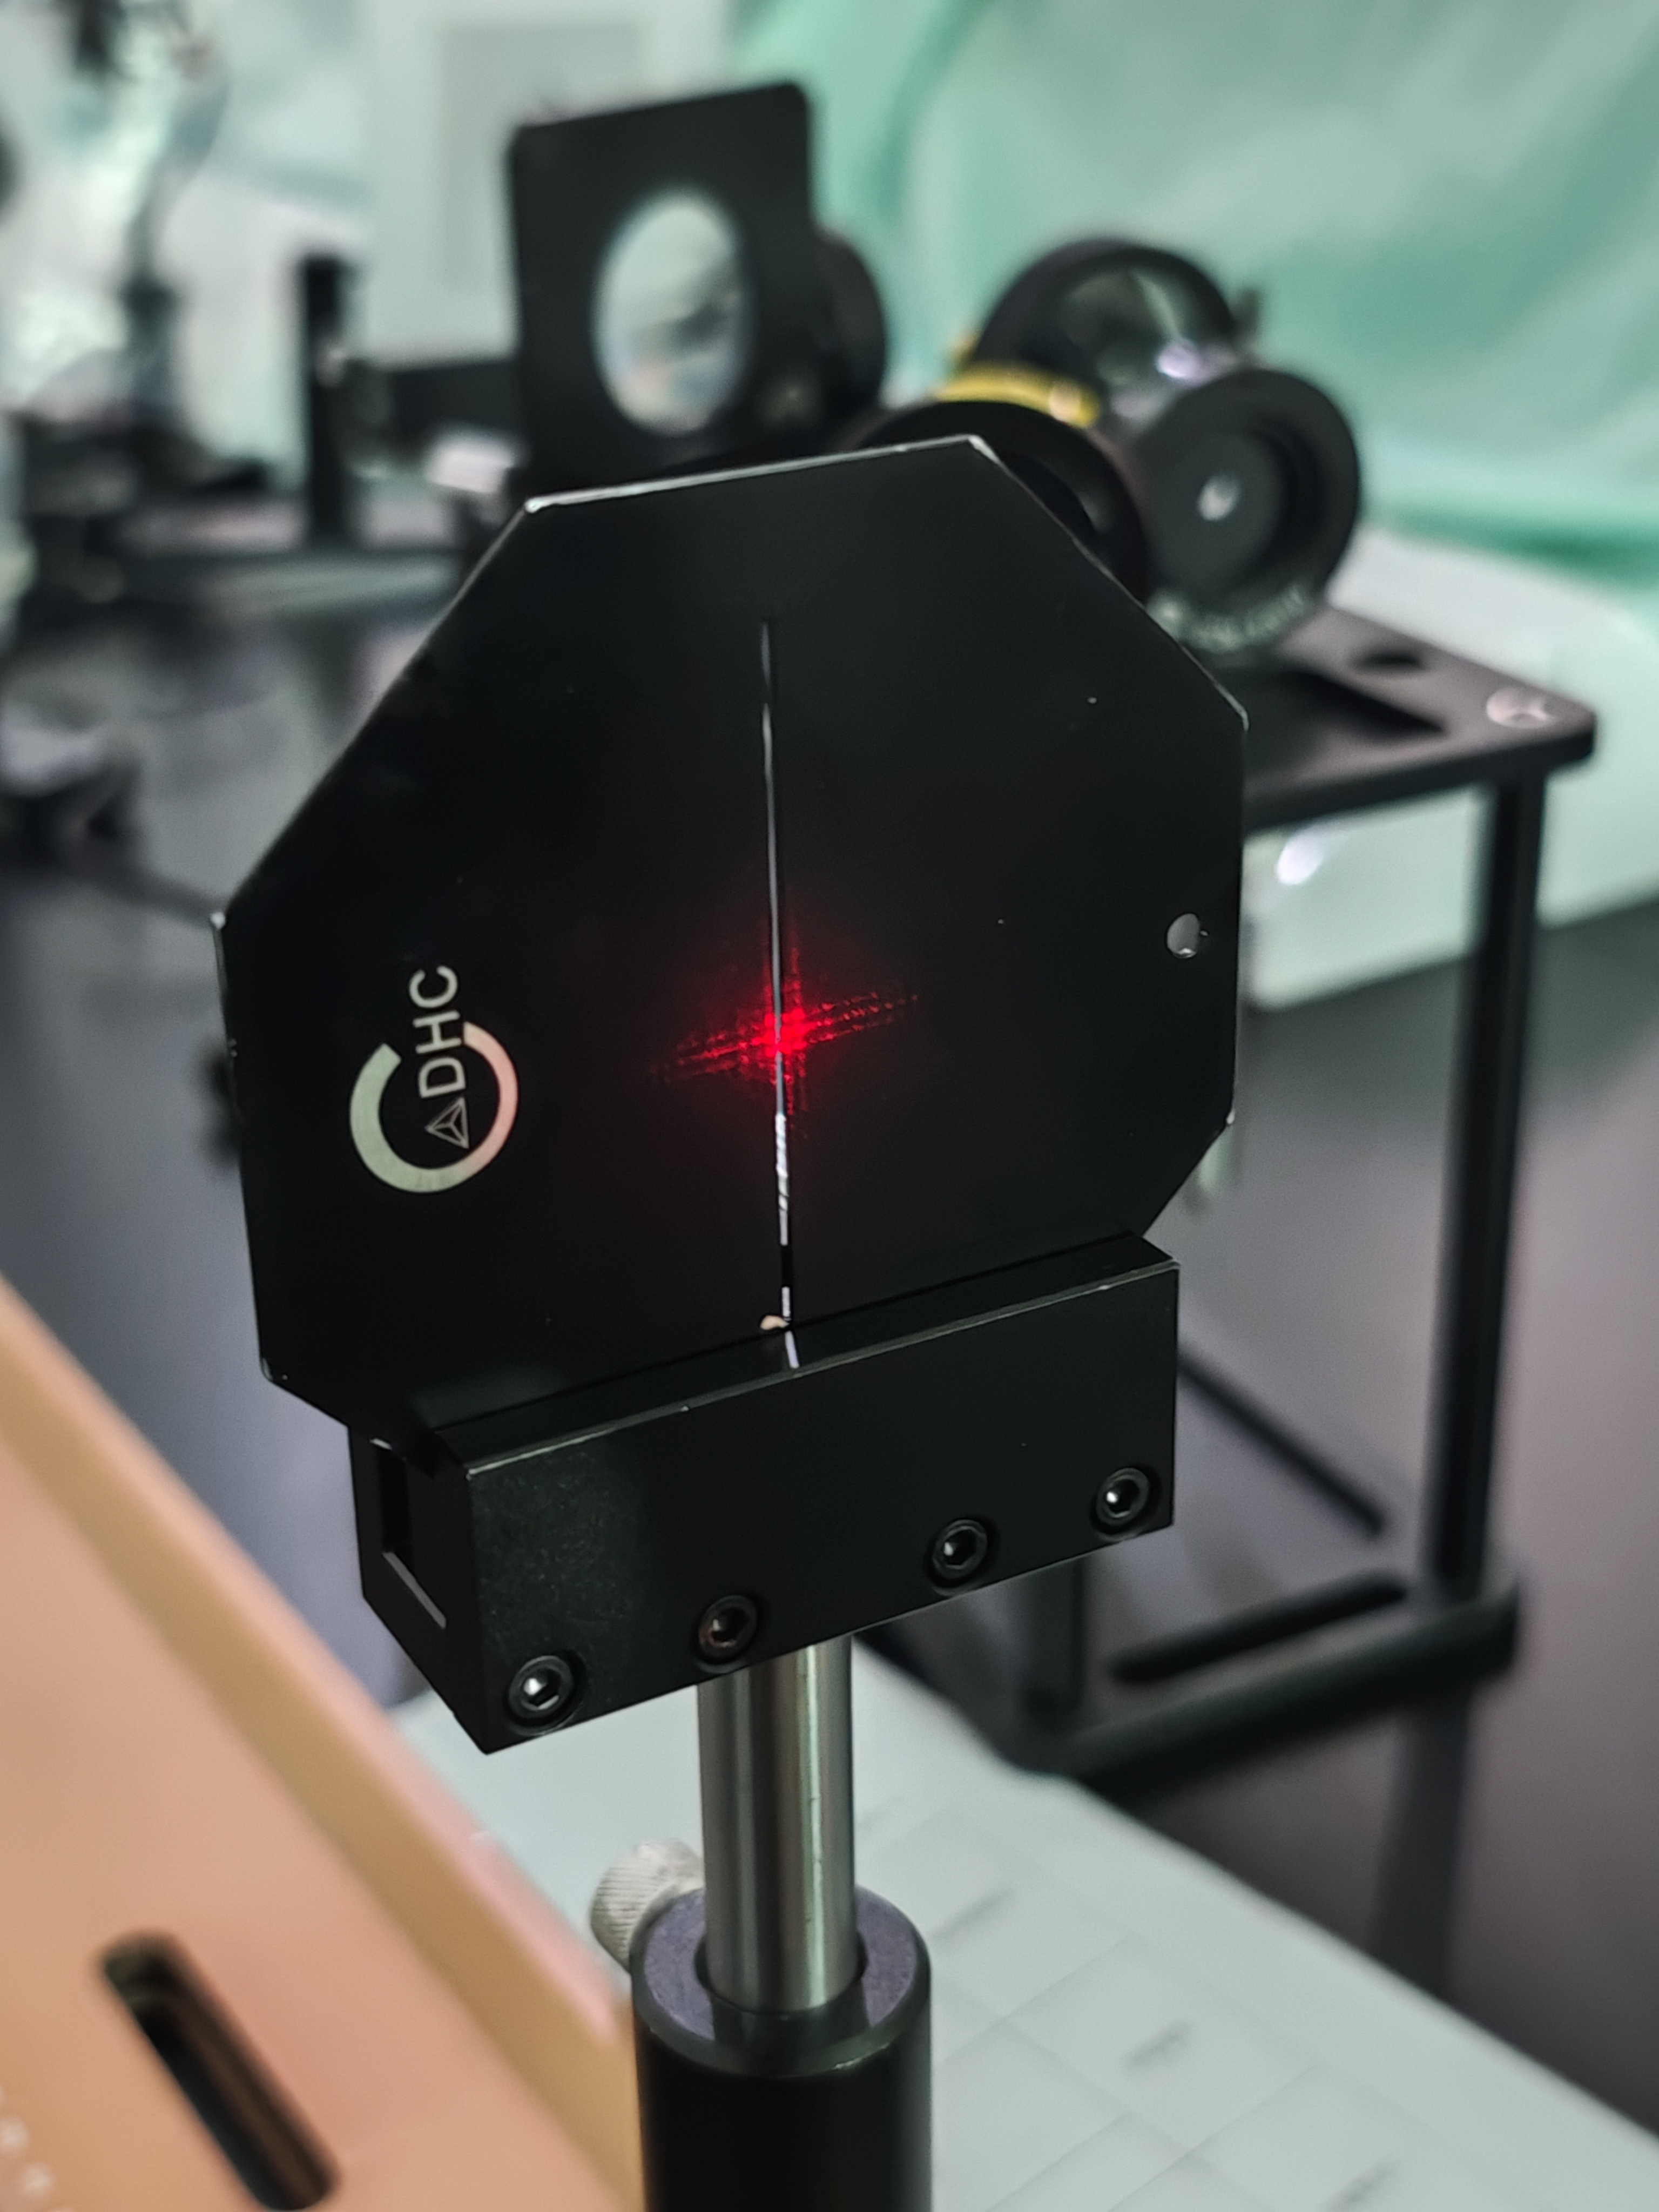
\includegraphics[width=0.25\textwidth]{fig17c.jpg}
    }
    \caption{阿贝尔成像实验图2}
    \label{fig:fig17}
\end{figure}
\paragraph{空间竖向滤波效果}在\ref{fig:fig17}方向滤波实验中，保留竖直条纹时，像面呈现明显的竖向条纹结构，横向细节丢失；
\begin{figure}[htbp]
    \centering
    \subfigure[光路图示]{
        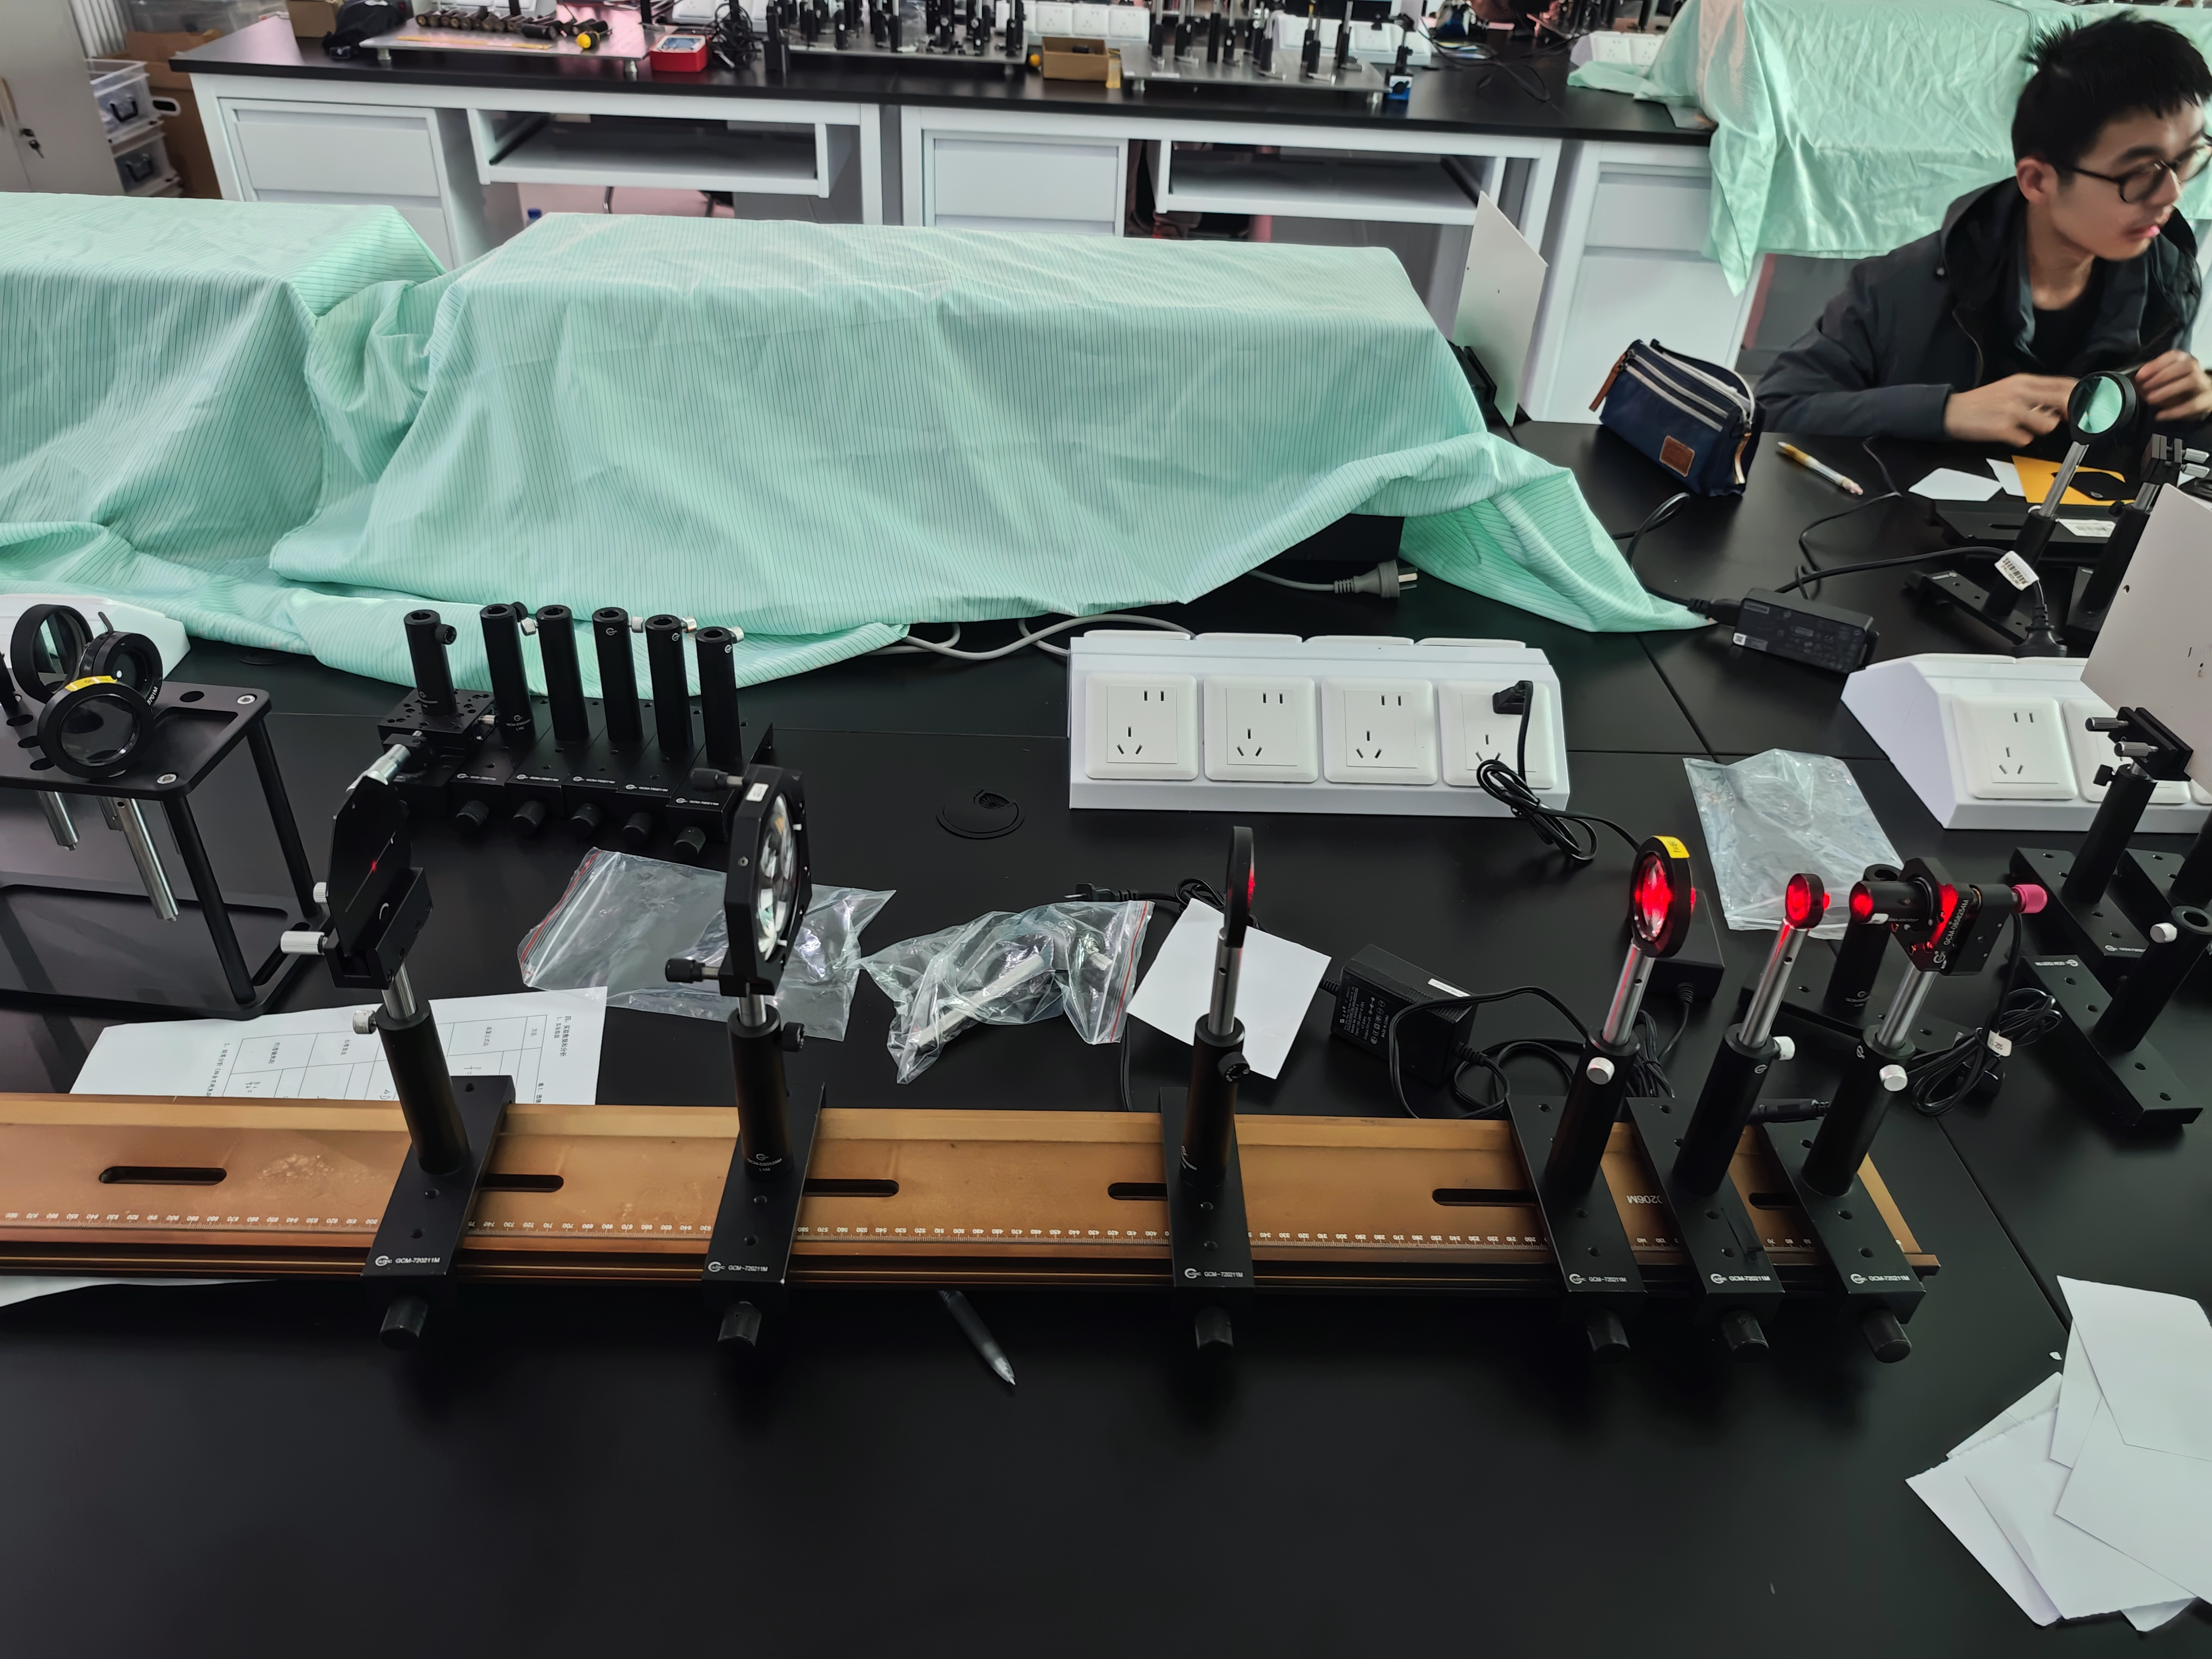
\includegraphics[width=0.25\textwidth]{fig18c.jpg}
    }
    \subfigure[成像]{
        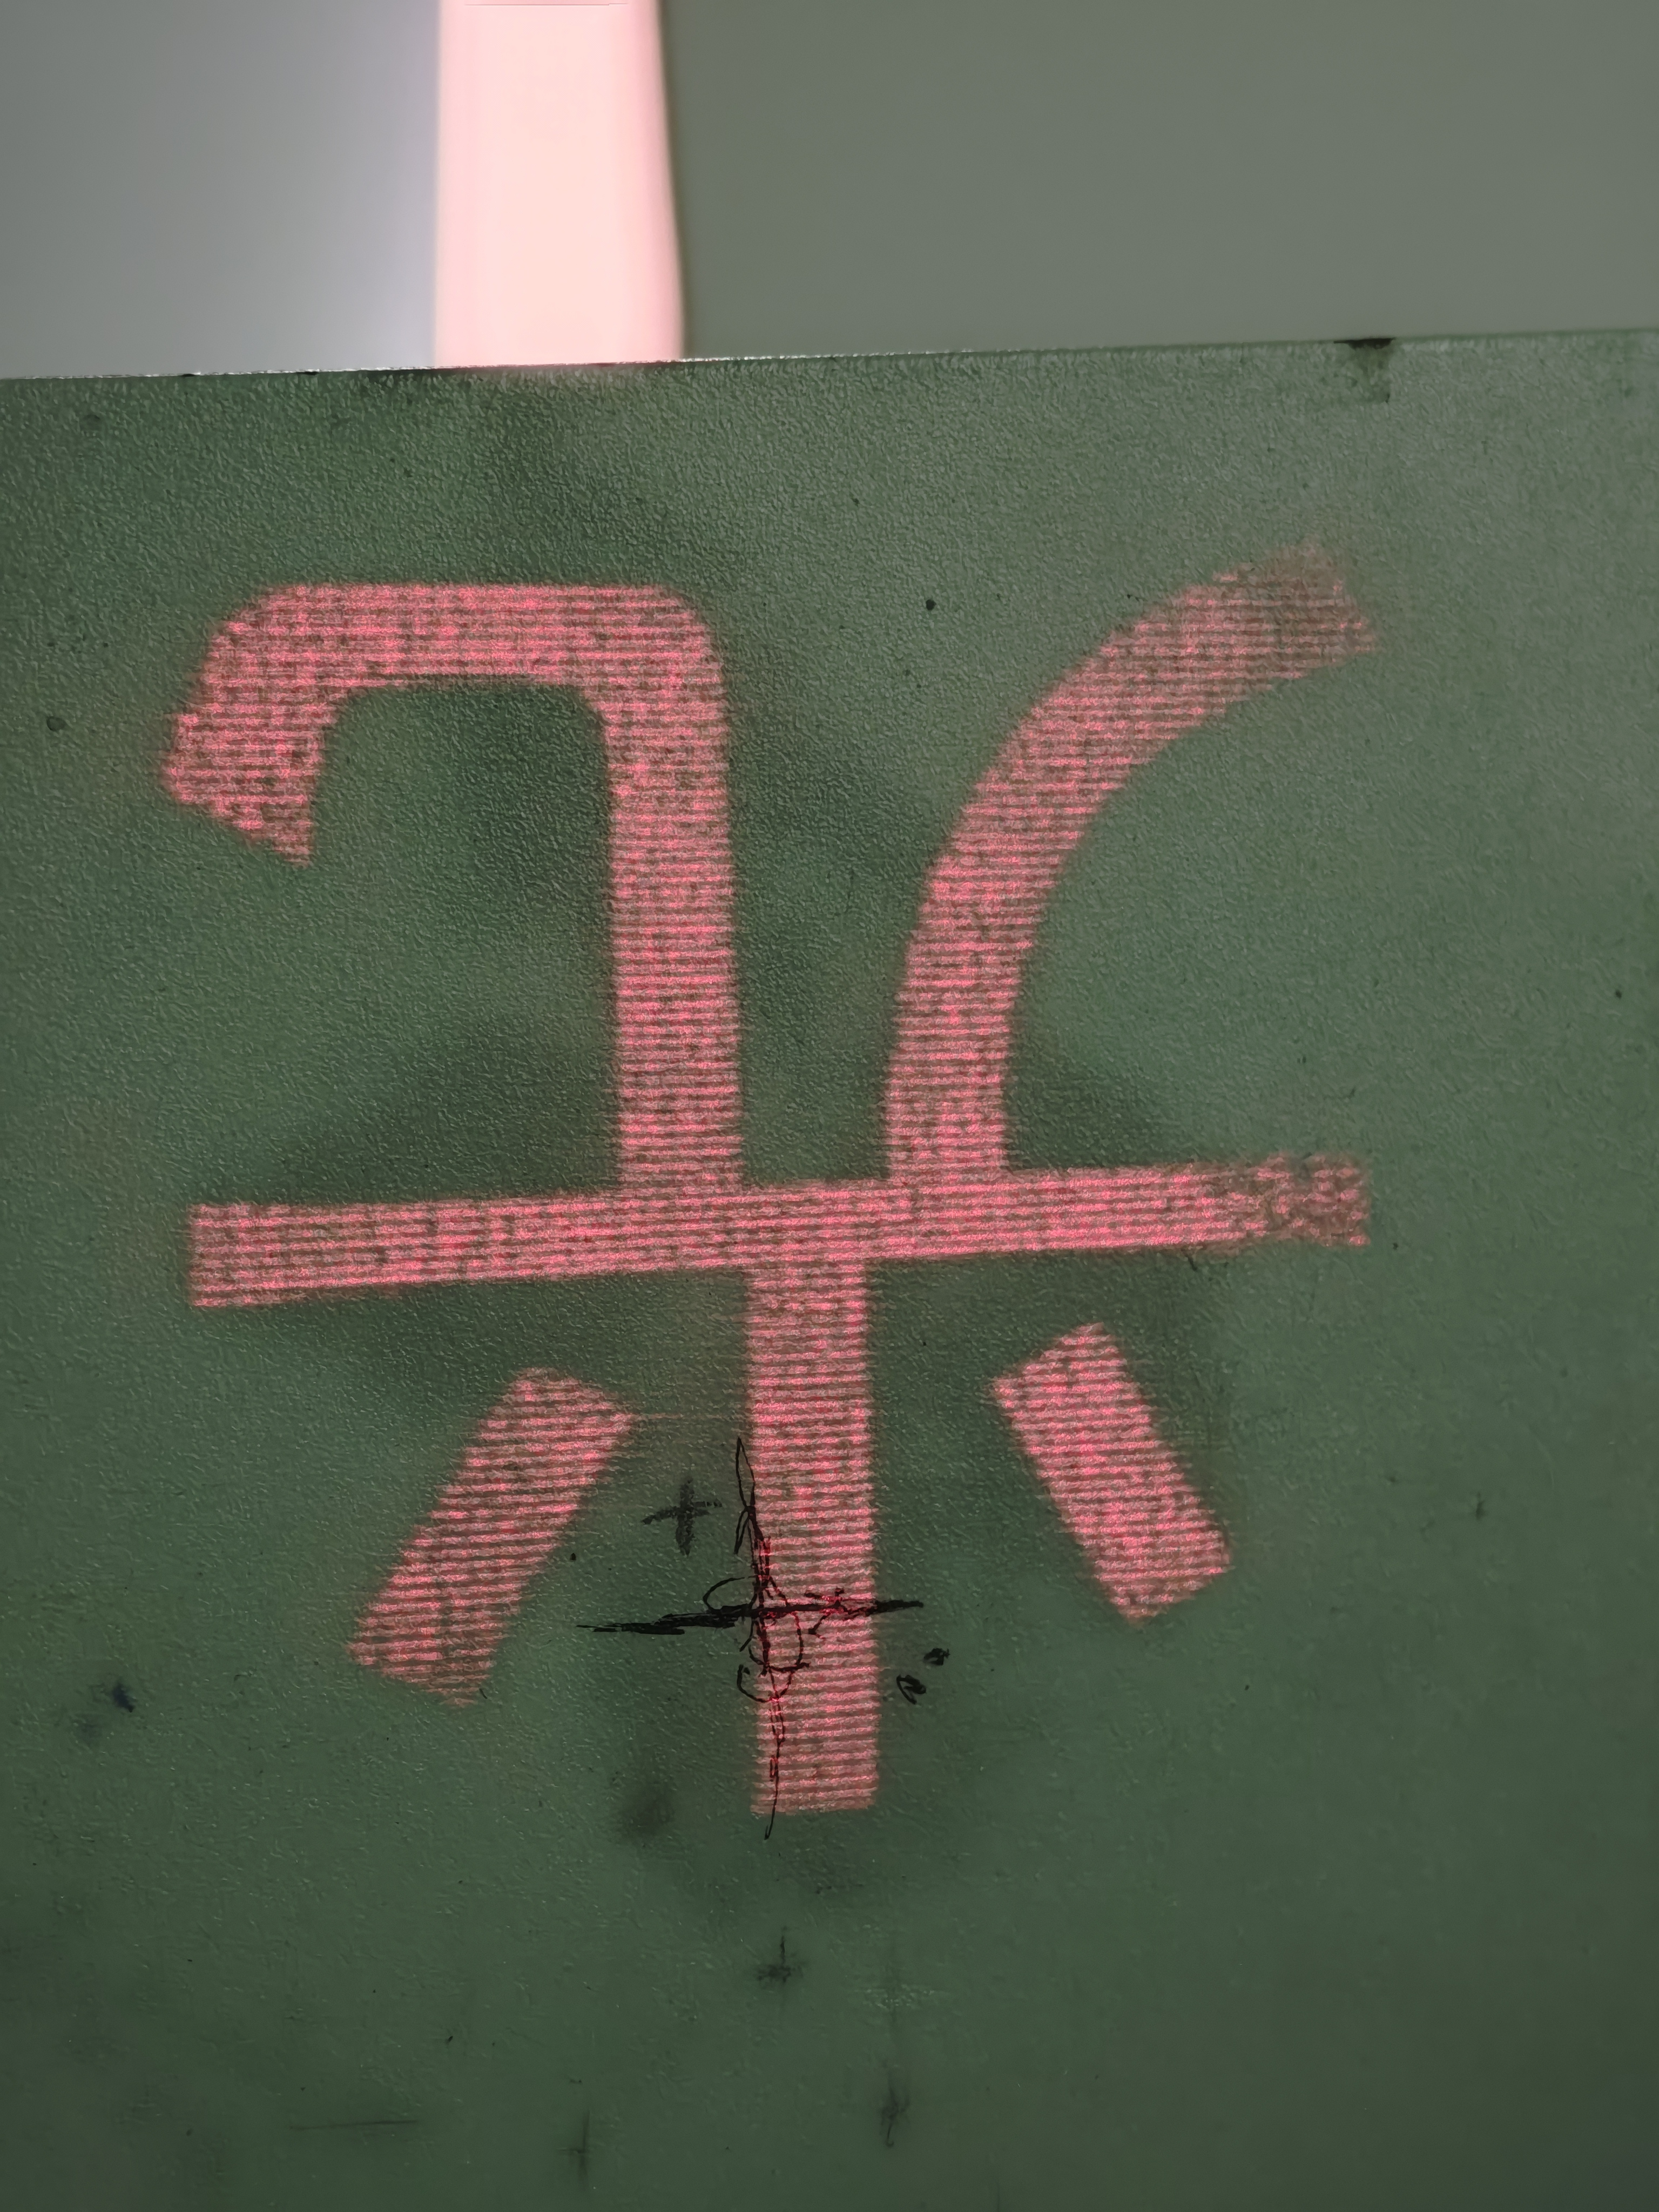
\includegraphics[width=0.25\textwidth]{fig18a.jpg}
    }
    \subfigure[频谱面图像]{
        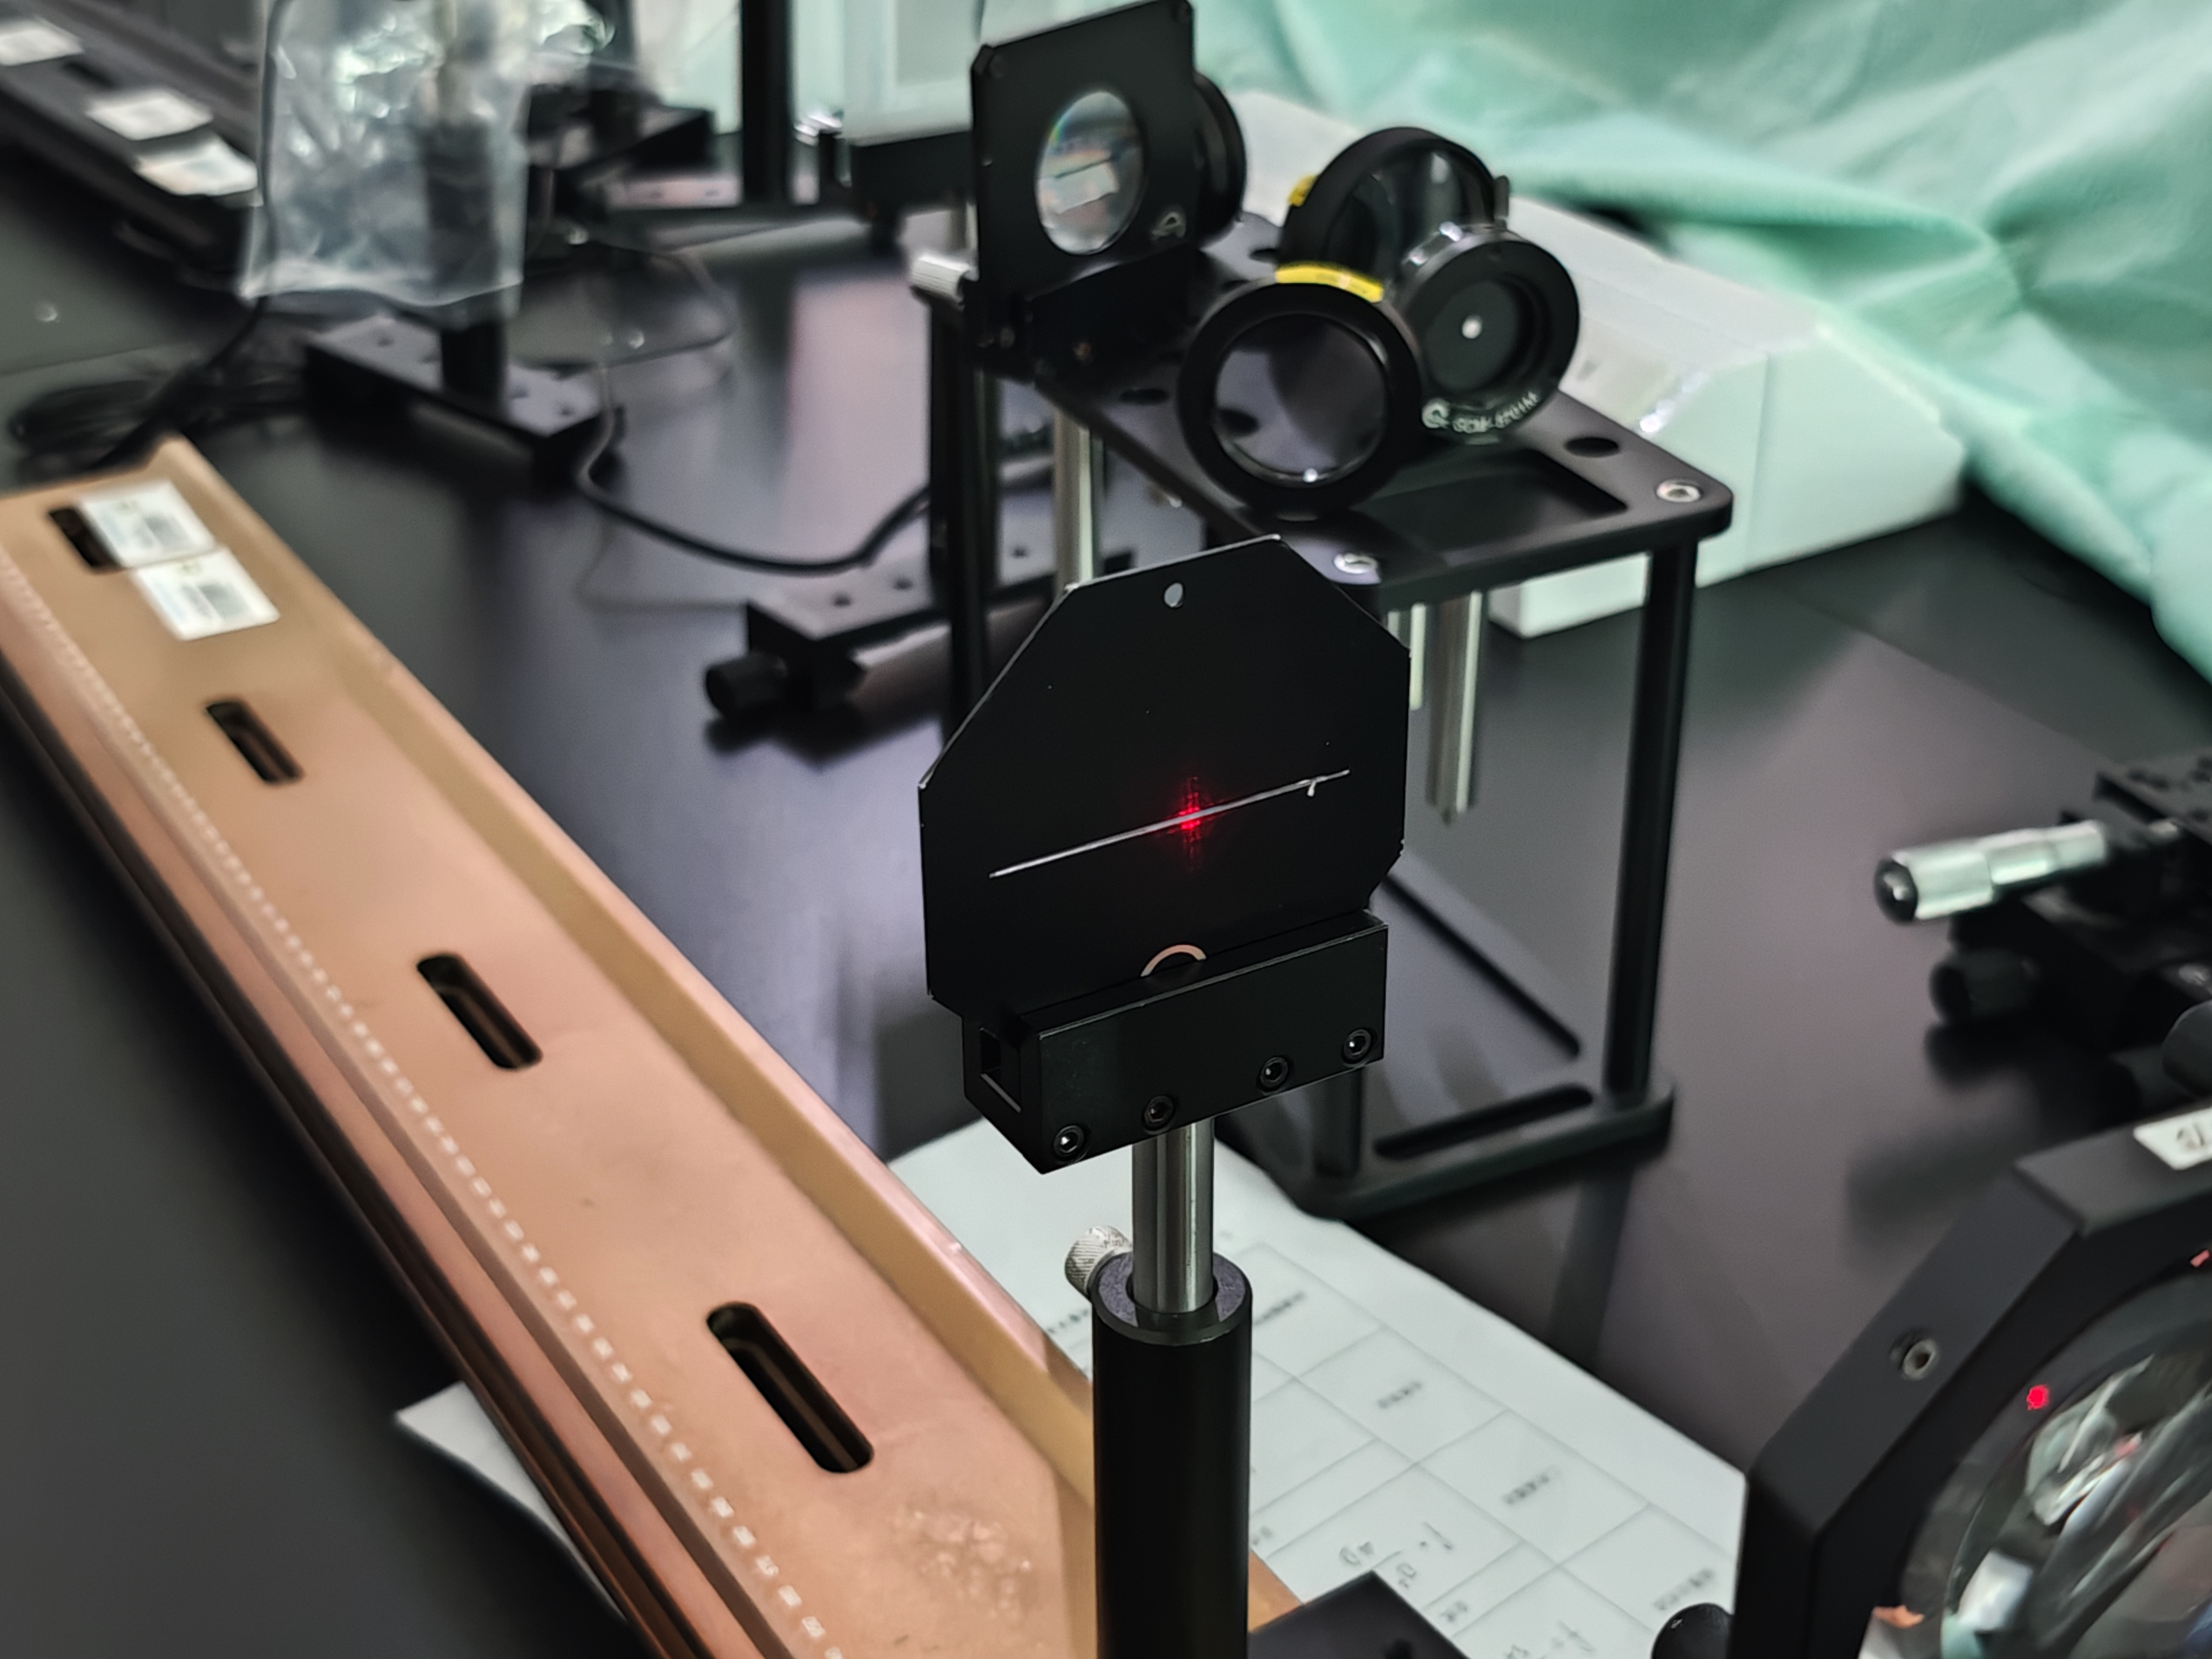
\includegraphics[width=0.25\textwidth]{fig18b.jpg}
    }
    \caption{阿贝尔成像实验图3}
    \label{fig:fig18}
\end{figure}
\paragraph{空间横向滤波效果}在图\ref{fig:fig18}方向滤波实验中，保留横向条纹时，像面呈现明显的横向条纹结构，竖向细节丢失；
\begin{figure}[!h]
    \centering
    \subfigure[光路图示]{
        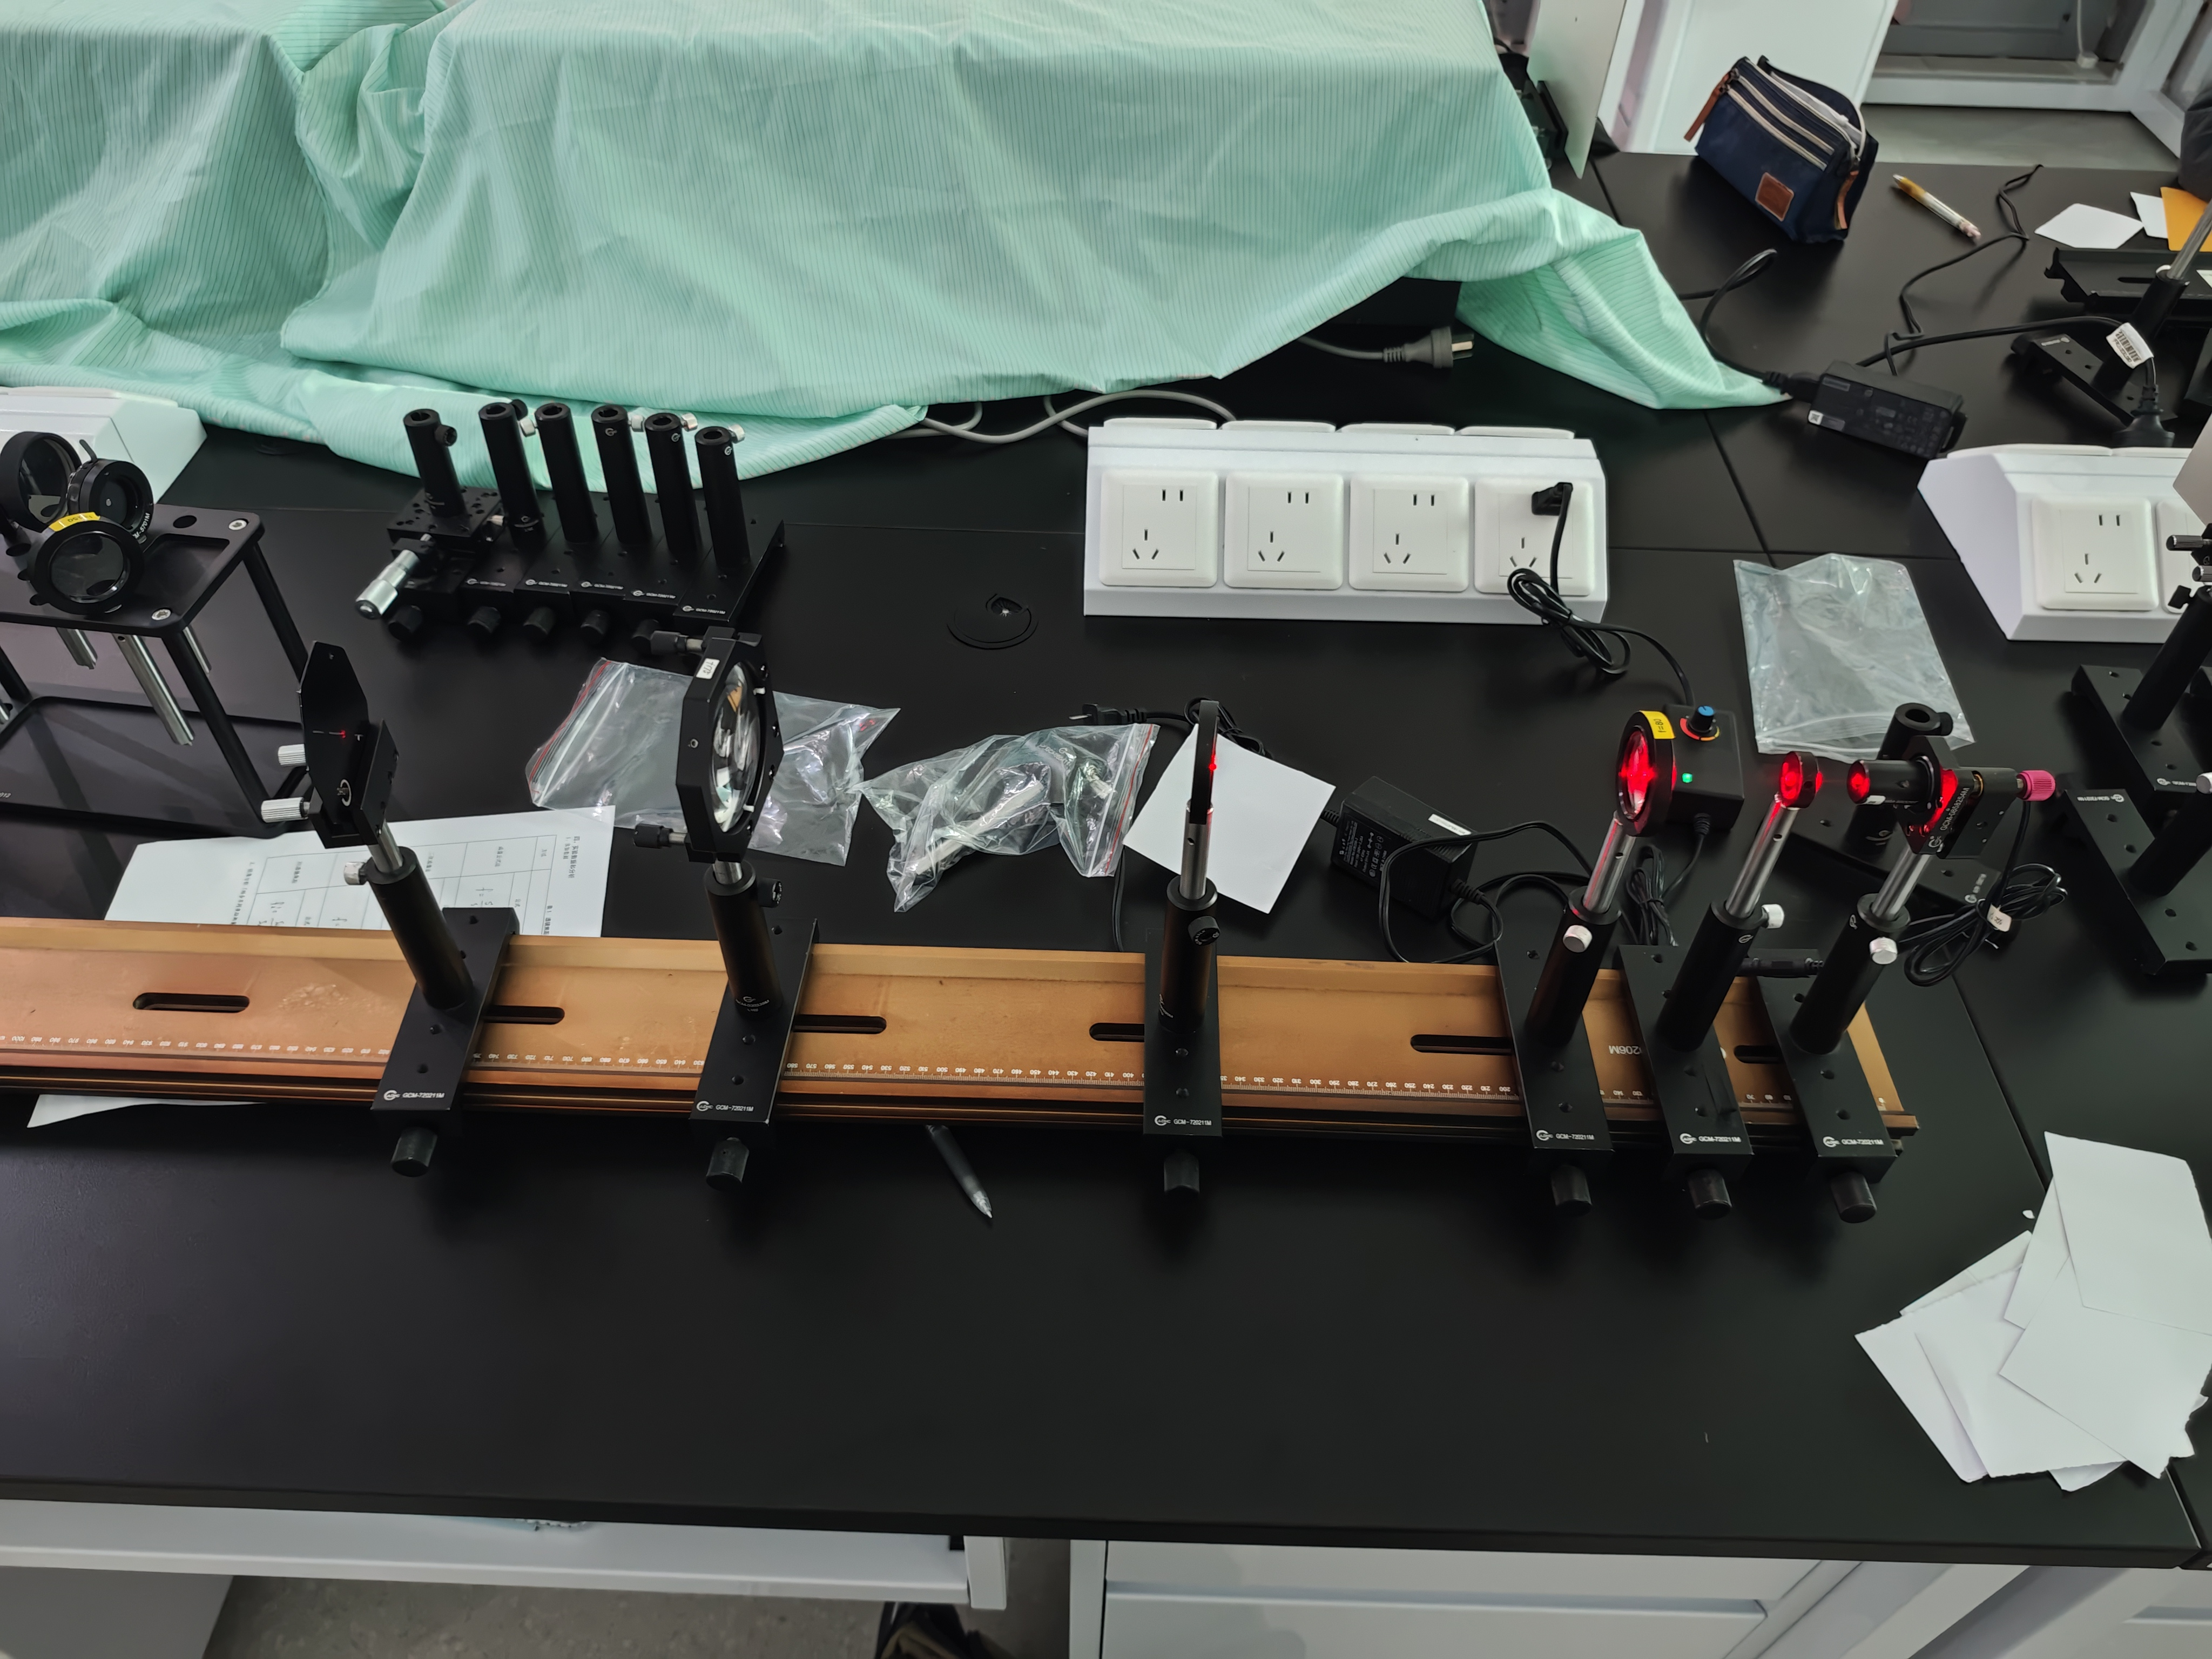
\includegraphics[width=0.25\textwidth]{fig19c.jpg}
    }
    \subfigure[成像]{
        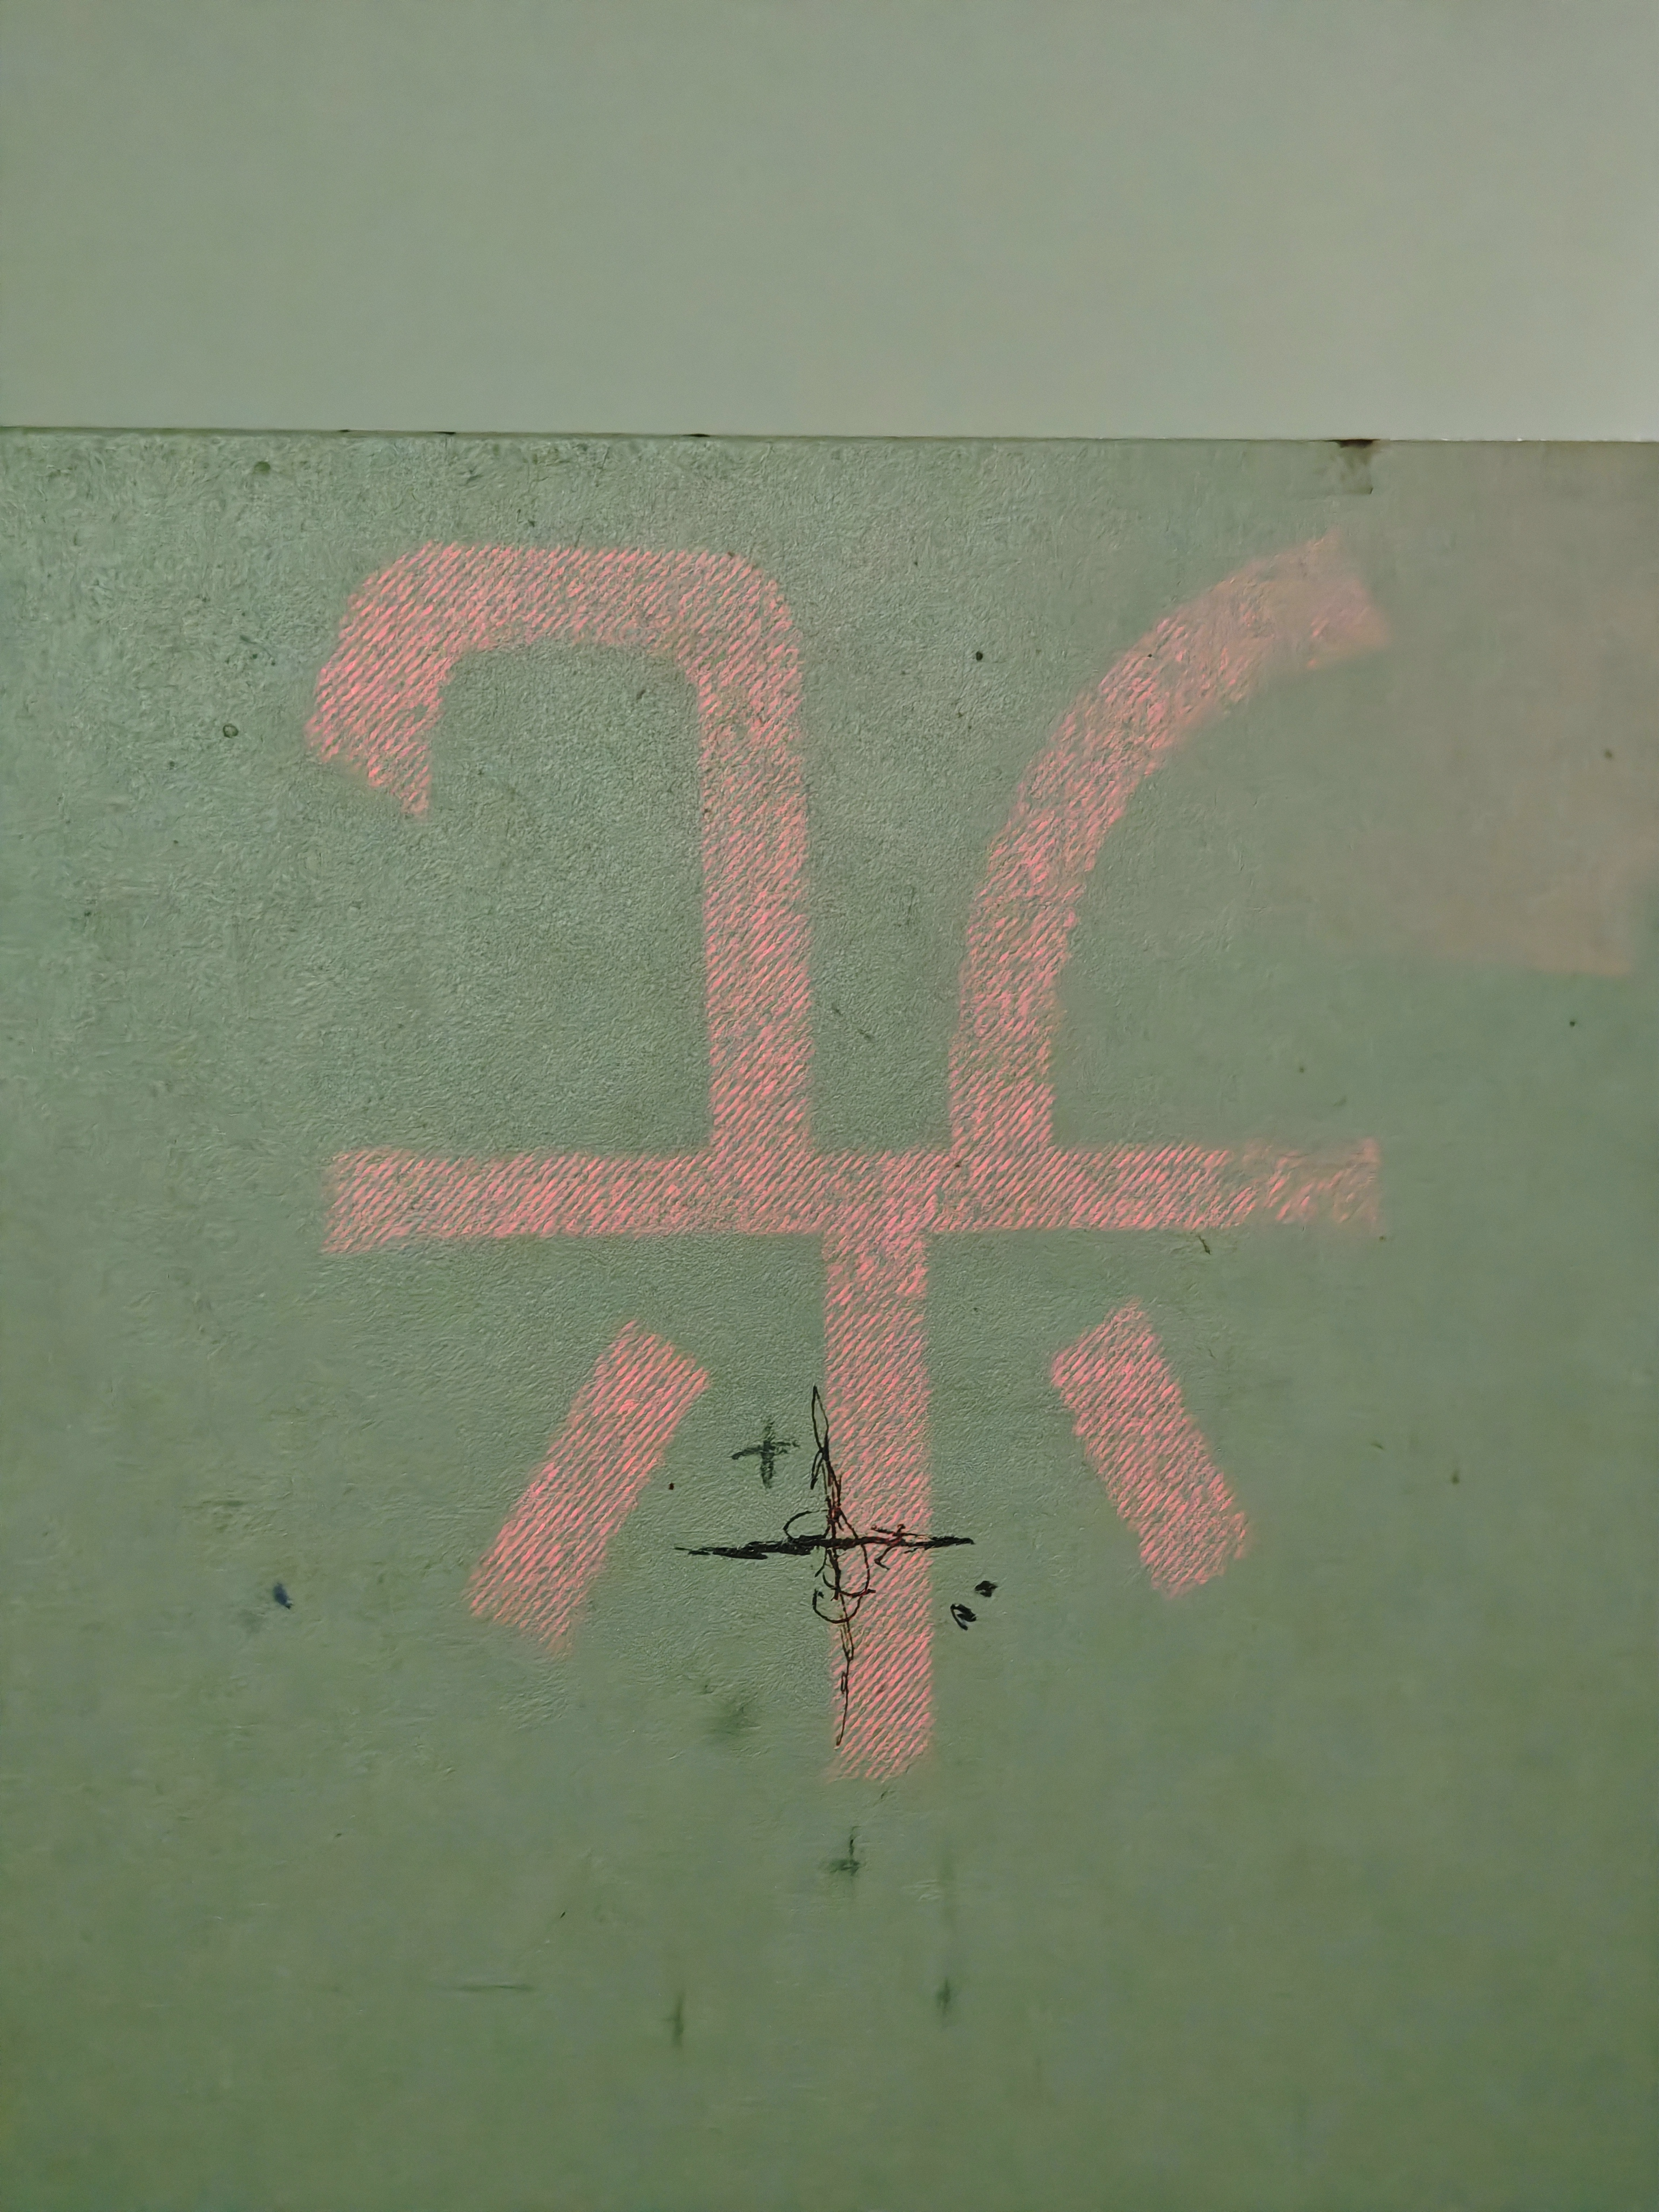
\includegraphics[width=0.25\textwidth]{fig19a.jpg}
    }
    \subfigure[频谱面图像]{
        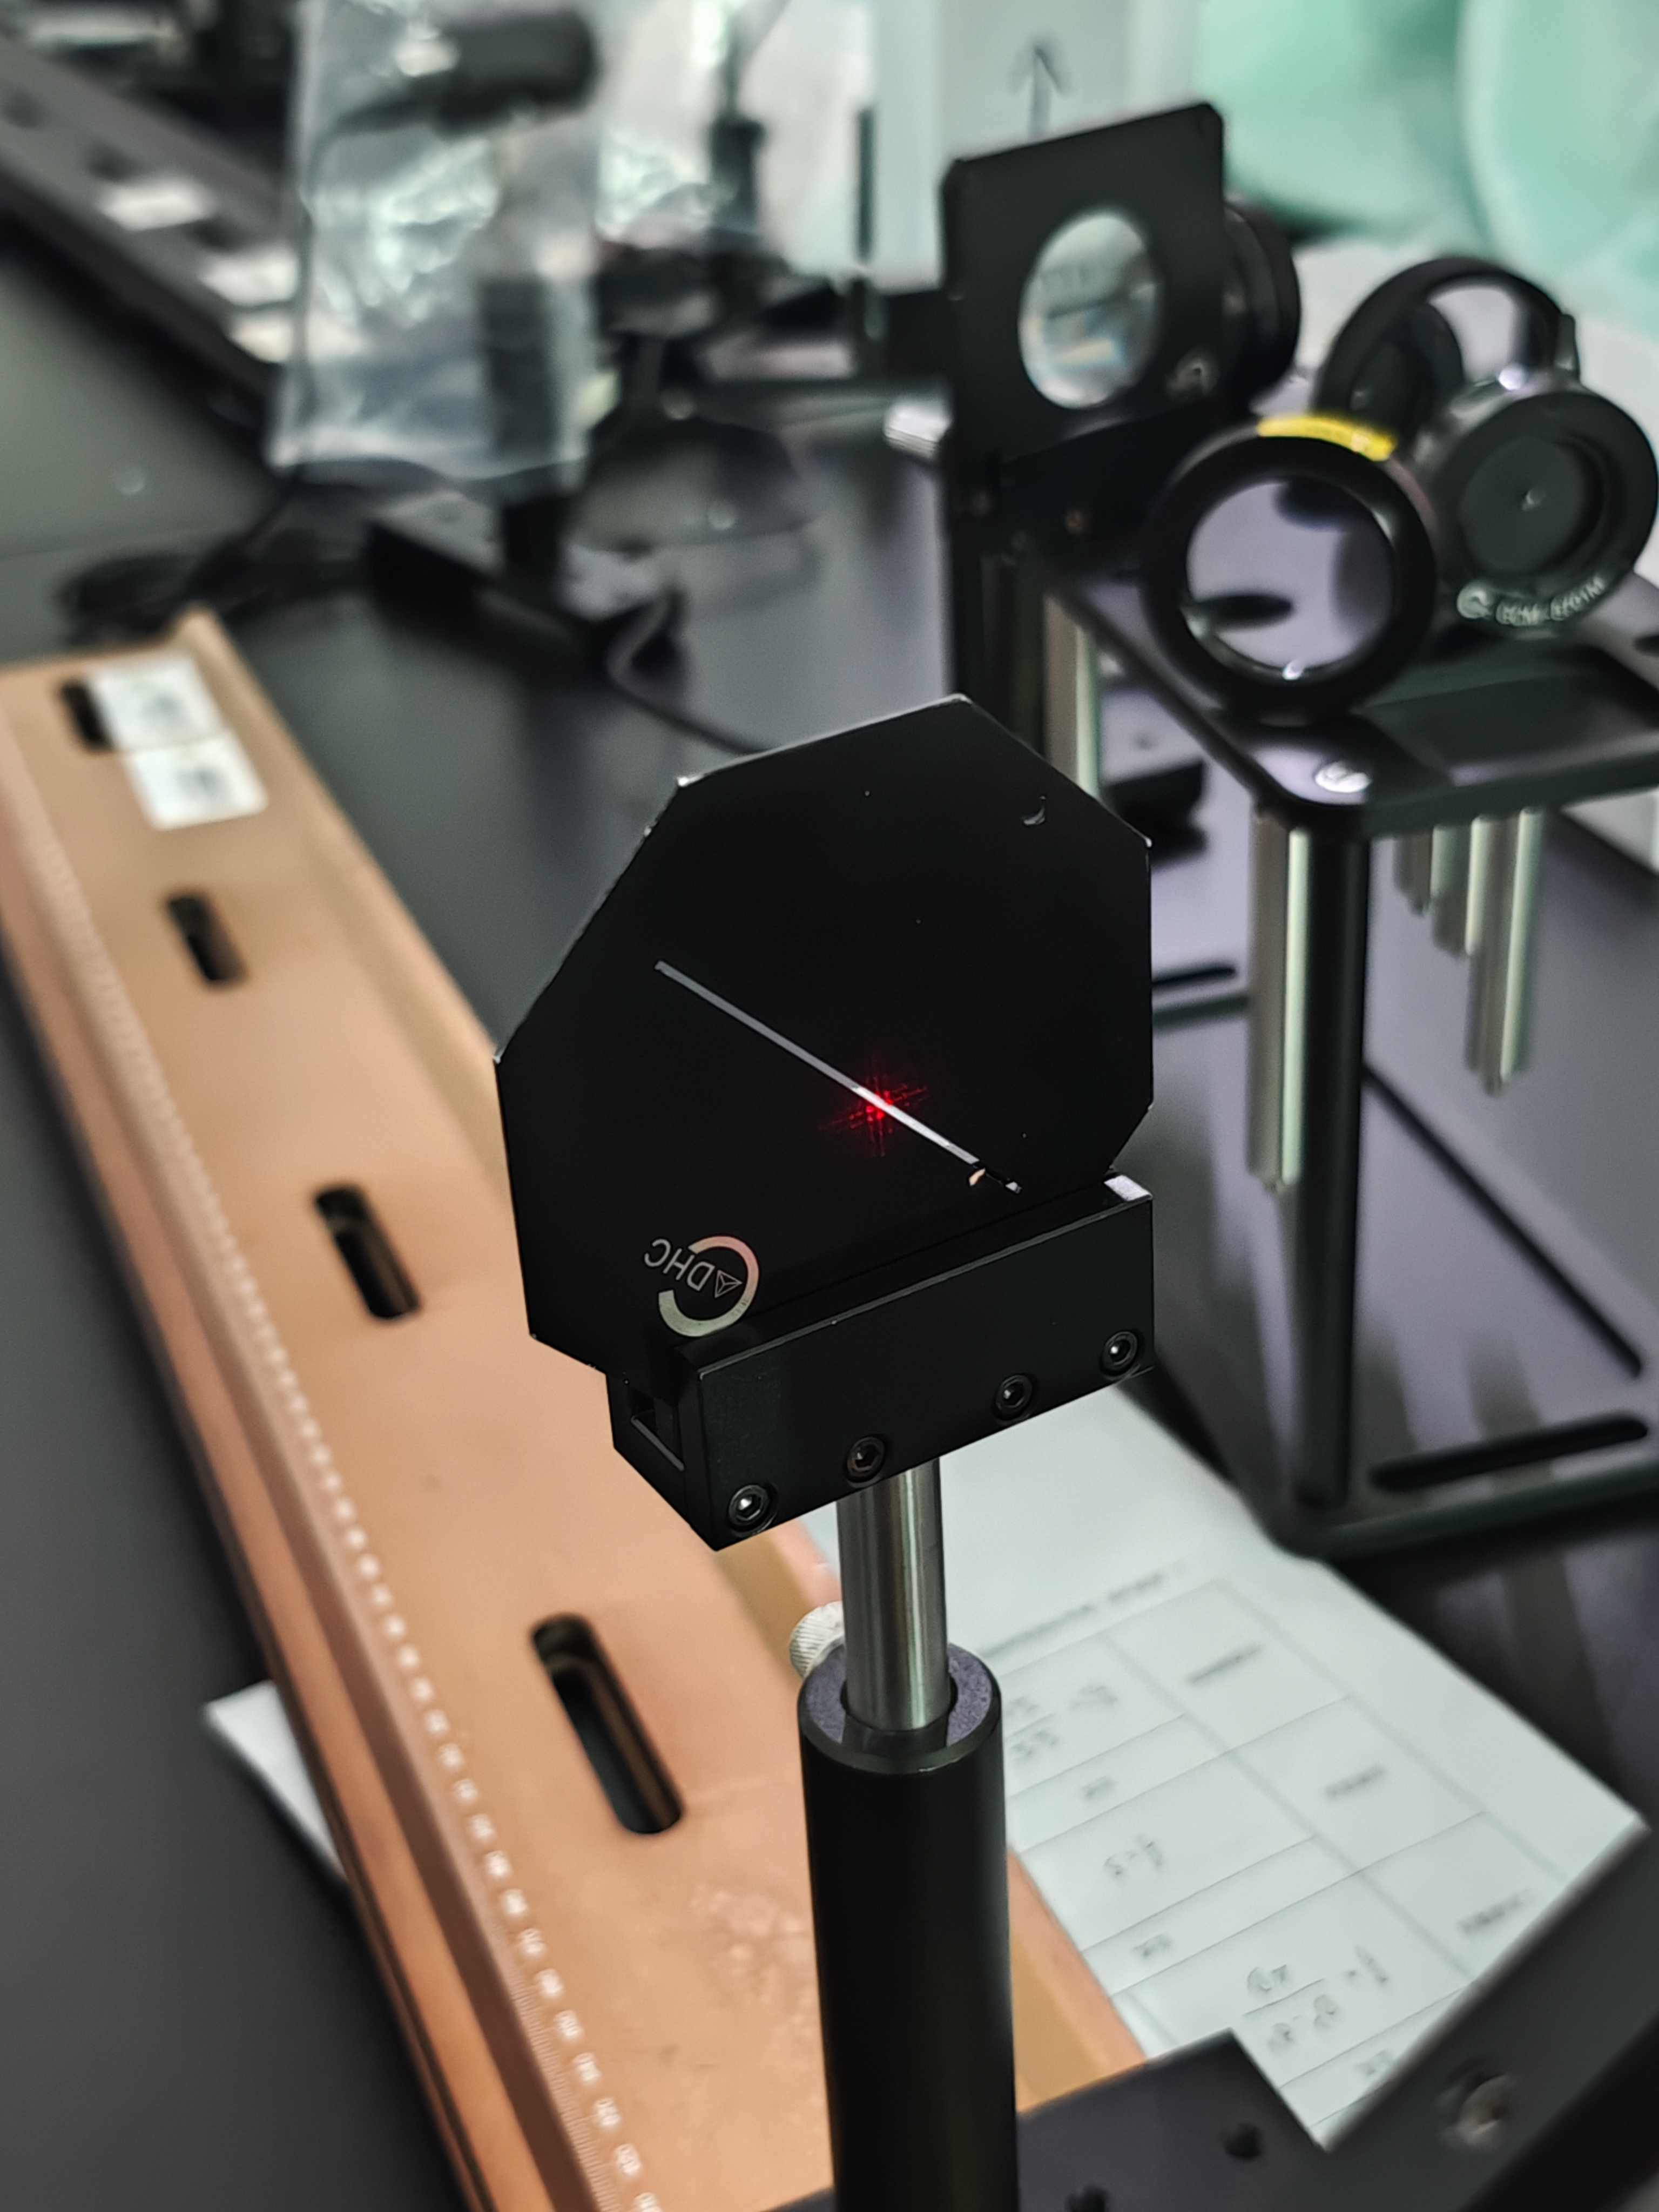
\includegraphics[width=0.25\textwidth]{fig19b.jpg}
    }
    \caption{阿贝尔成像实验图4}
    \label{fig:fig19}
\end{figure}
\paragraph{空间45°滤波效果}在图\ref{fig:fig19}方向滤波实验中，保留45°斜向条纹时，像面呈现明显的斜向条纹结构，与之相竖直的方向的细节丢失；

\begin{figure}[!h]
    \centering
    \subfigure[光路图示]{
        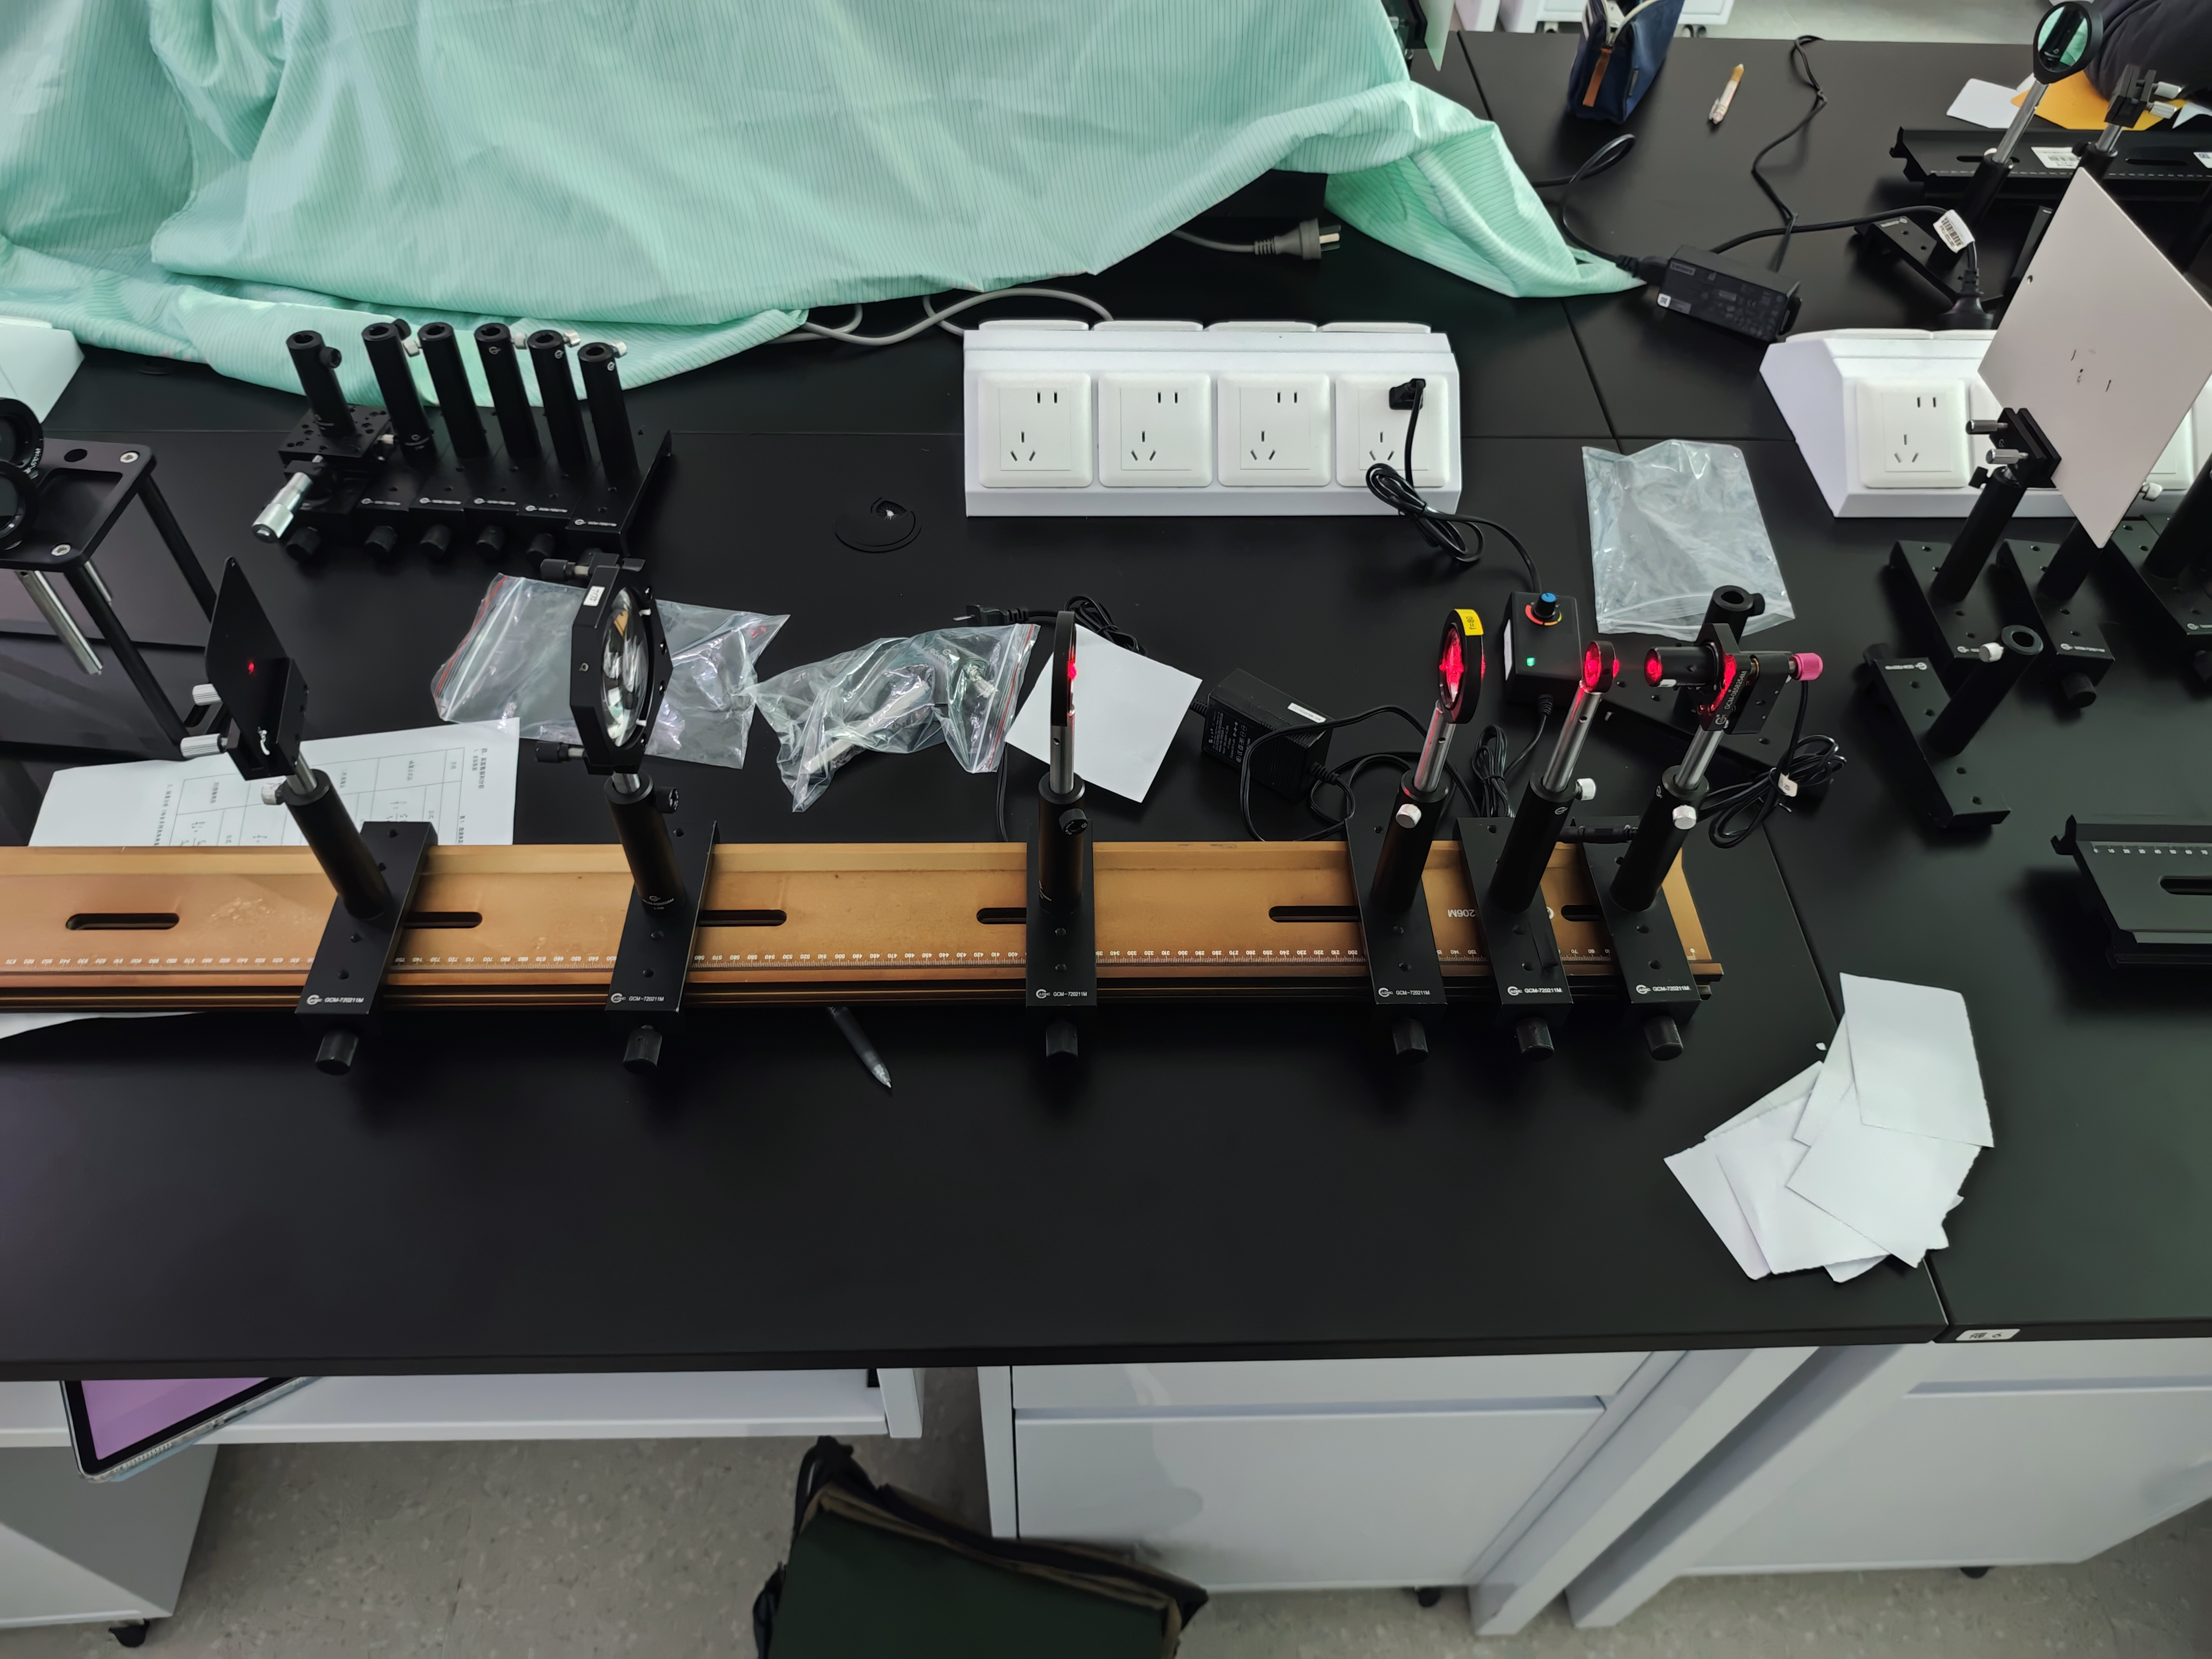
\includegraphics[width=0.25\textwidth]{IMG_20251105_153910.jpg}
    }
    \subfigure[成像]{
        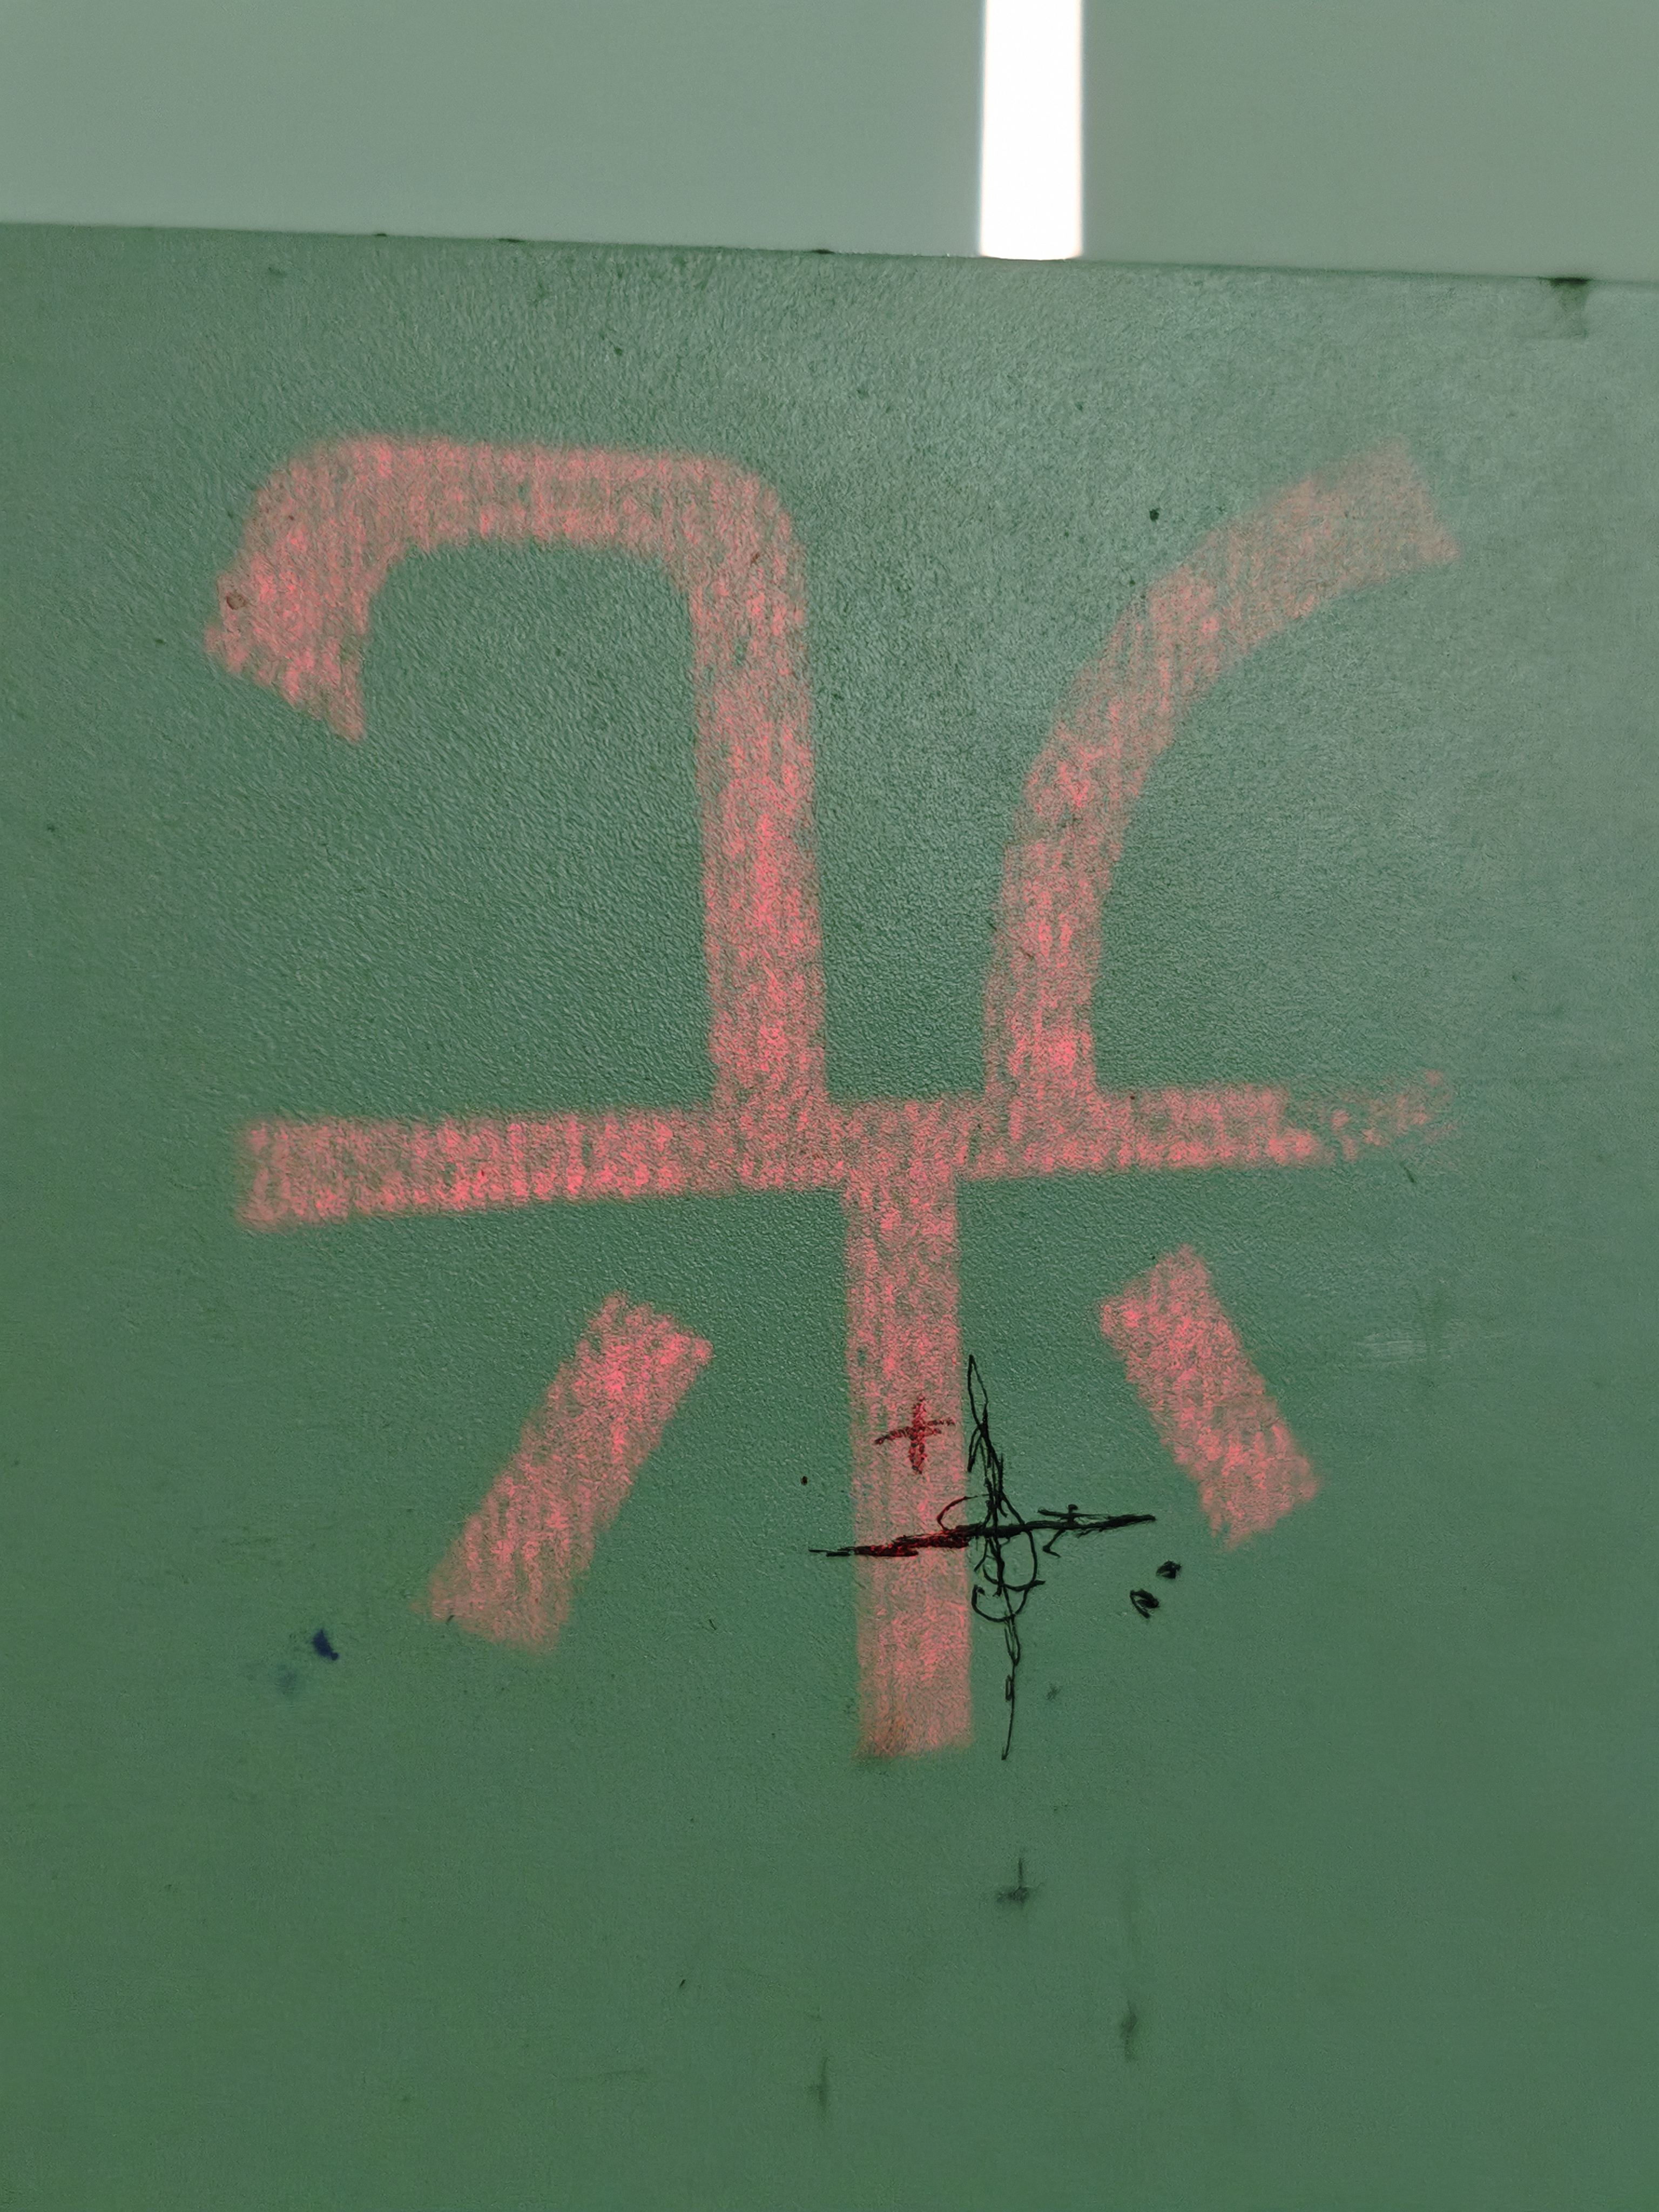
\includegraphics[width=0.25\textwidth]{IMG_20251105_153858.jpg}
    }
    \subfigure[频谱面图像]{
        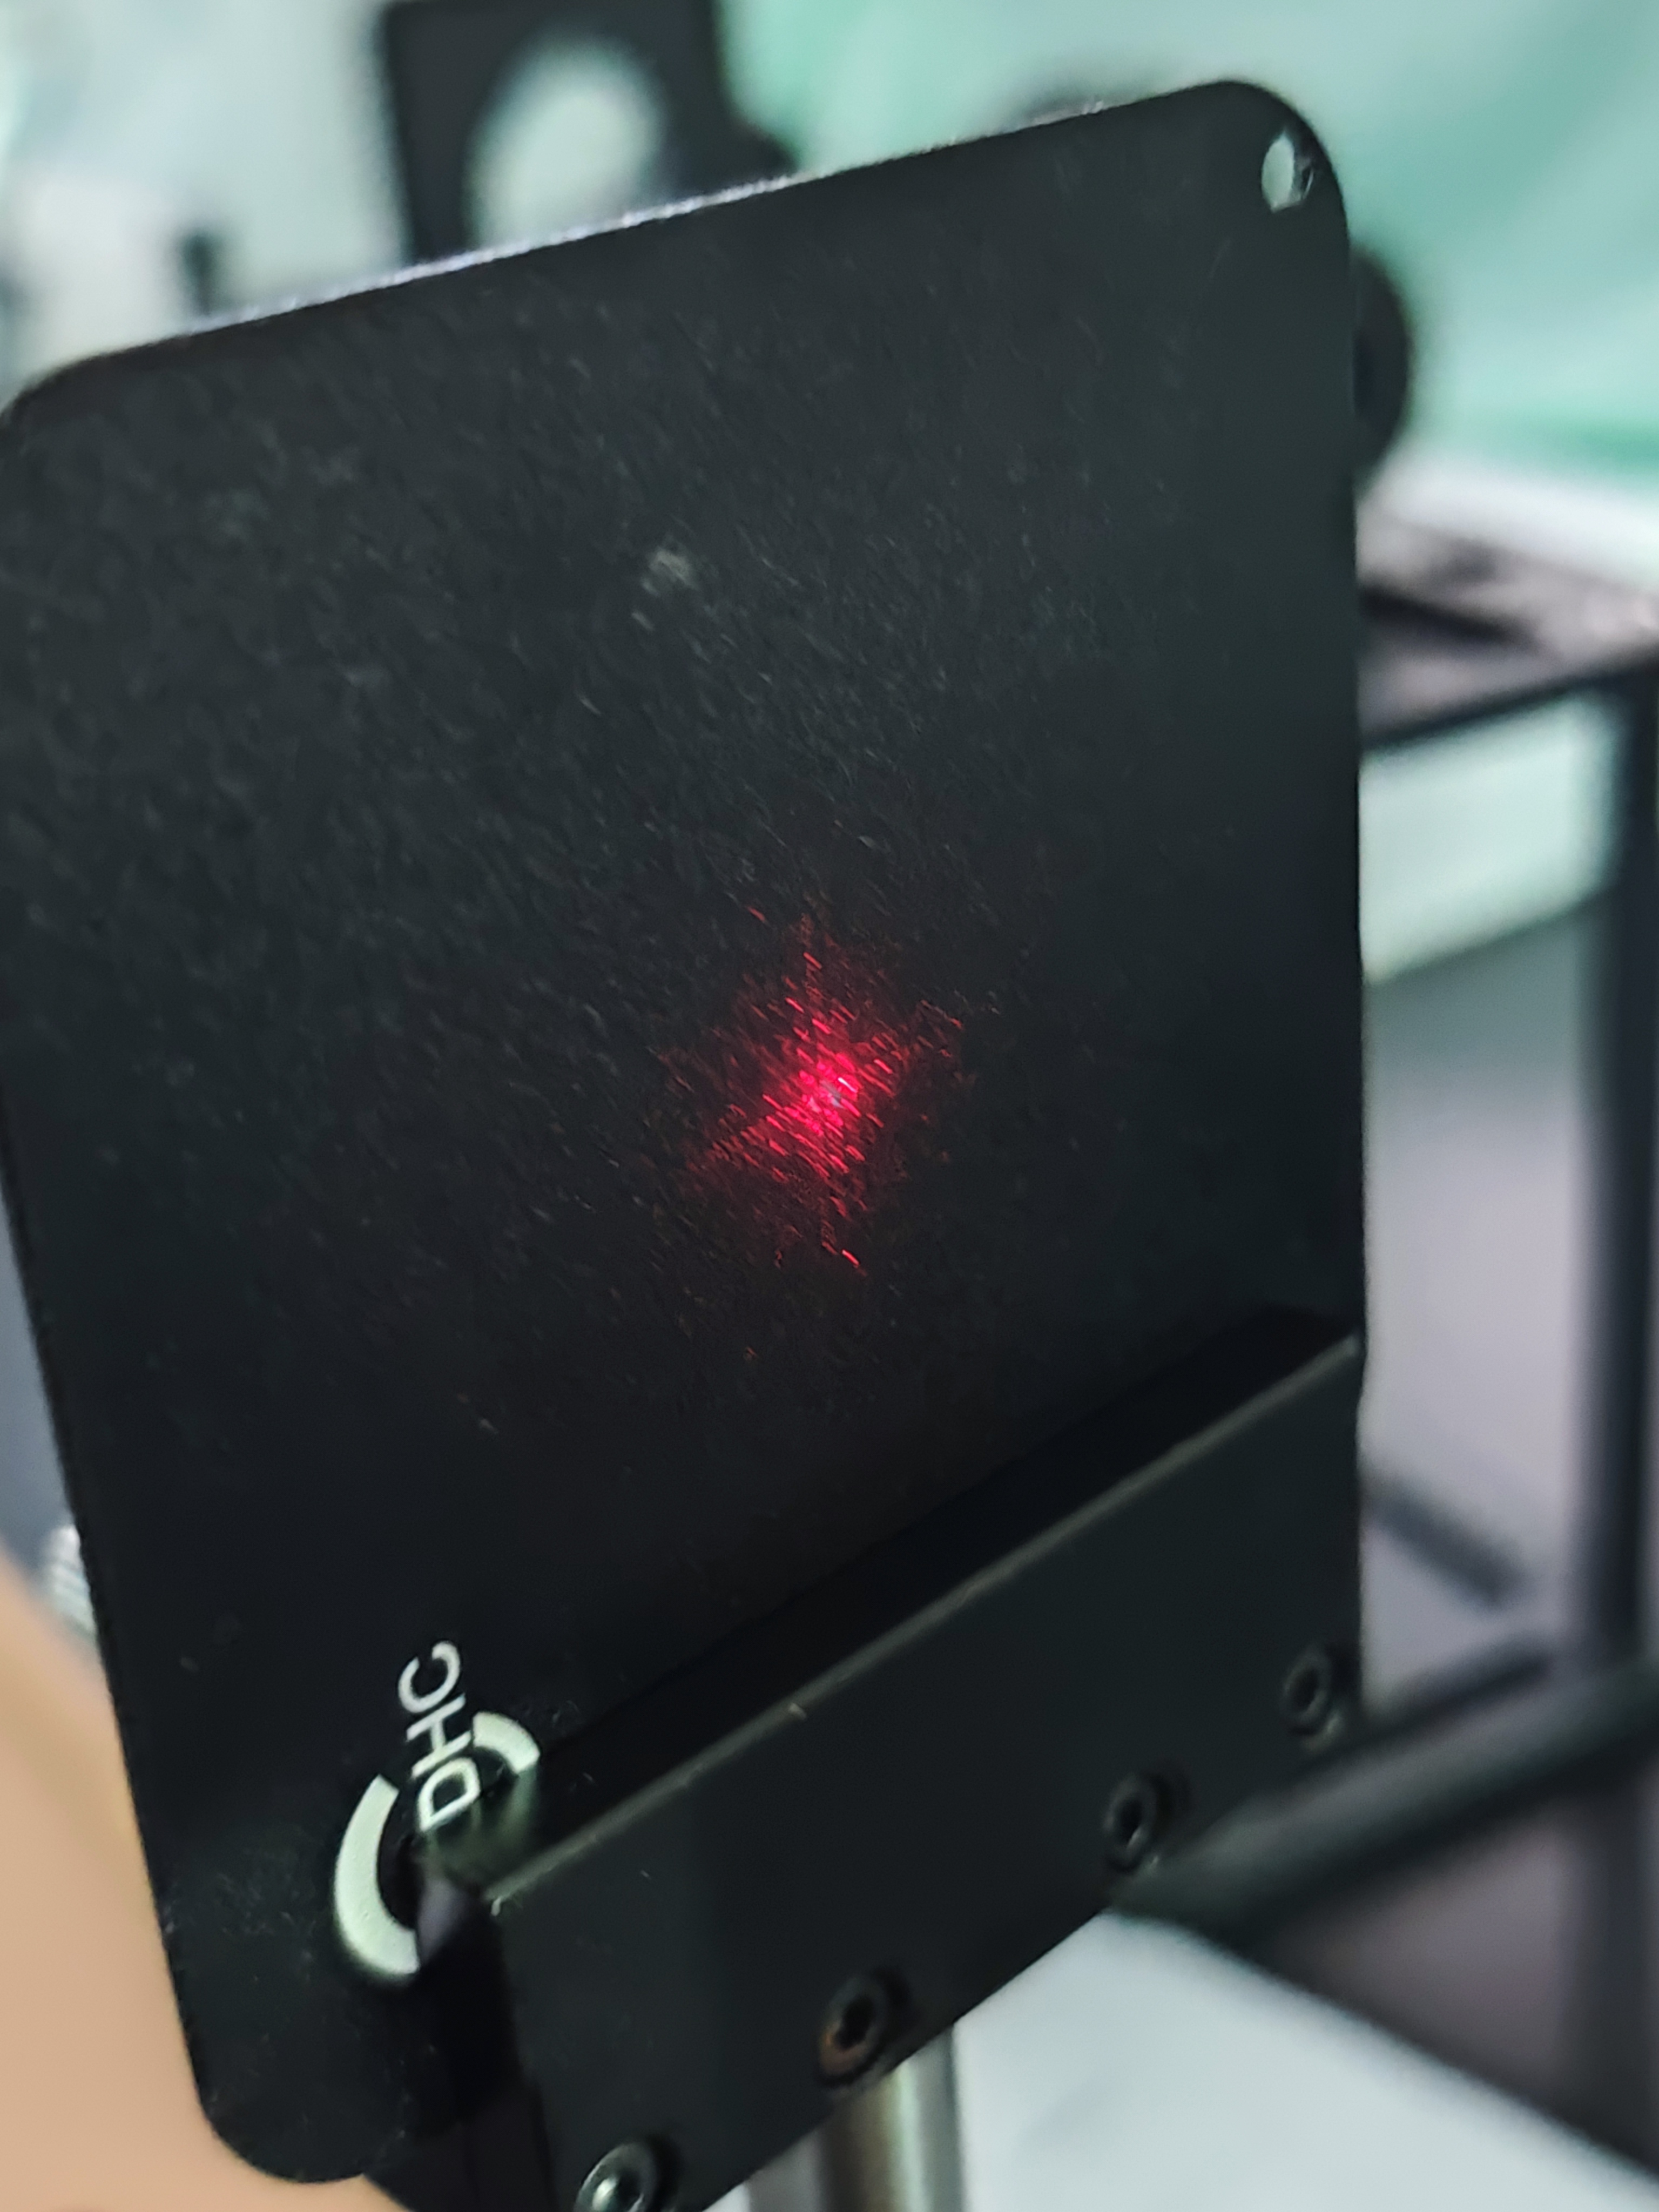
\includegraphics[width=0.25\textwidth]{IMG_20251105_153905.jpg}
    }
    \caption{阿贝尔成像实验图5}
    \label{fig:fig20}
\end{figure}
\paragraph{高通滤波实验}在图\ref{fig:fig20}高通滤波实验中，阻挡0级频谱点后，像面显示出“光”字的轮廓边缘，背景变暗，实现了边缘提取效果。

\clearpage
\subsection{光学4F系统成像结果}
在4F系统中，如图\ref{fig:fig21}和\ref{fig:fig22}成功实现了物体的1:1成像，像面清晰显示了物孔的倒立实像。
\begin{figure}[!htbp]
    \centering
    \subfigure[光路图示]{
        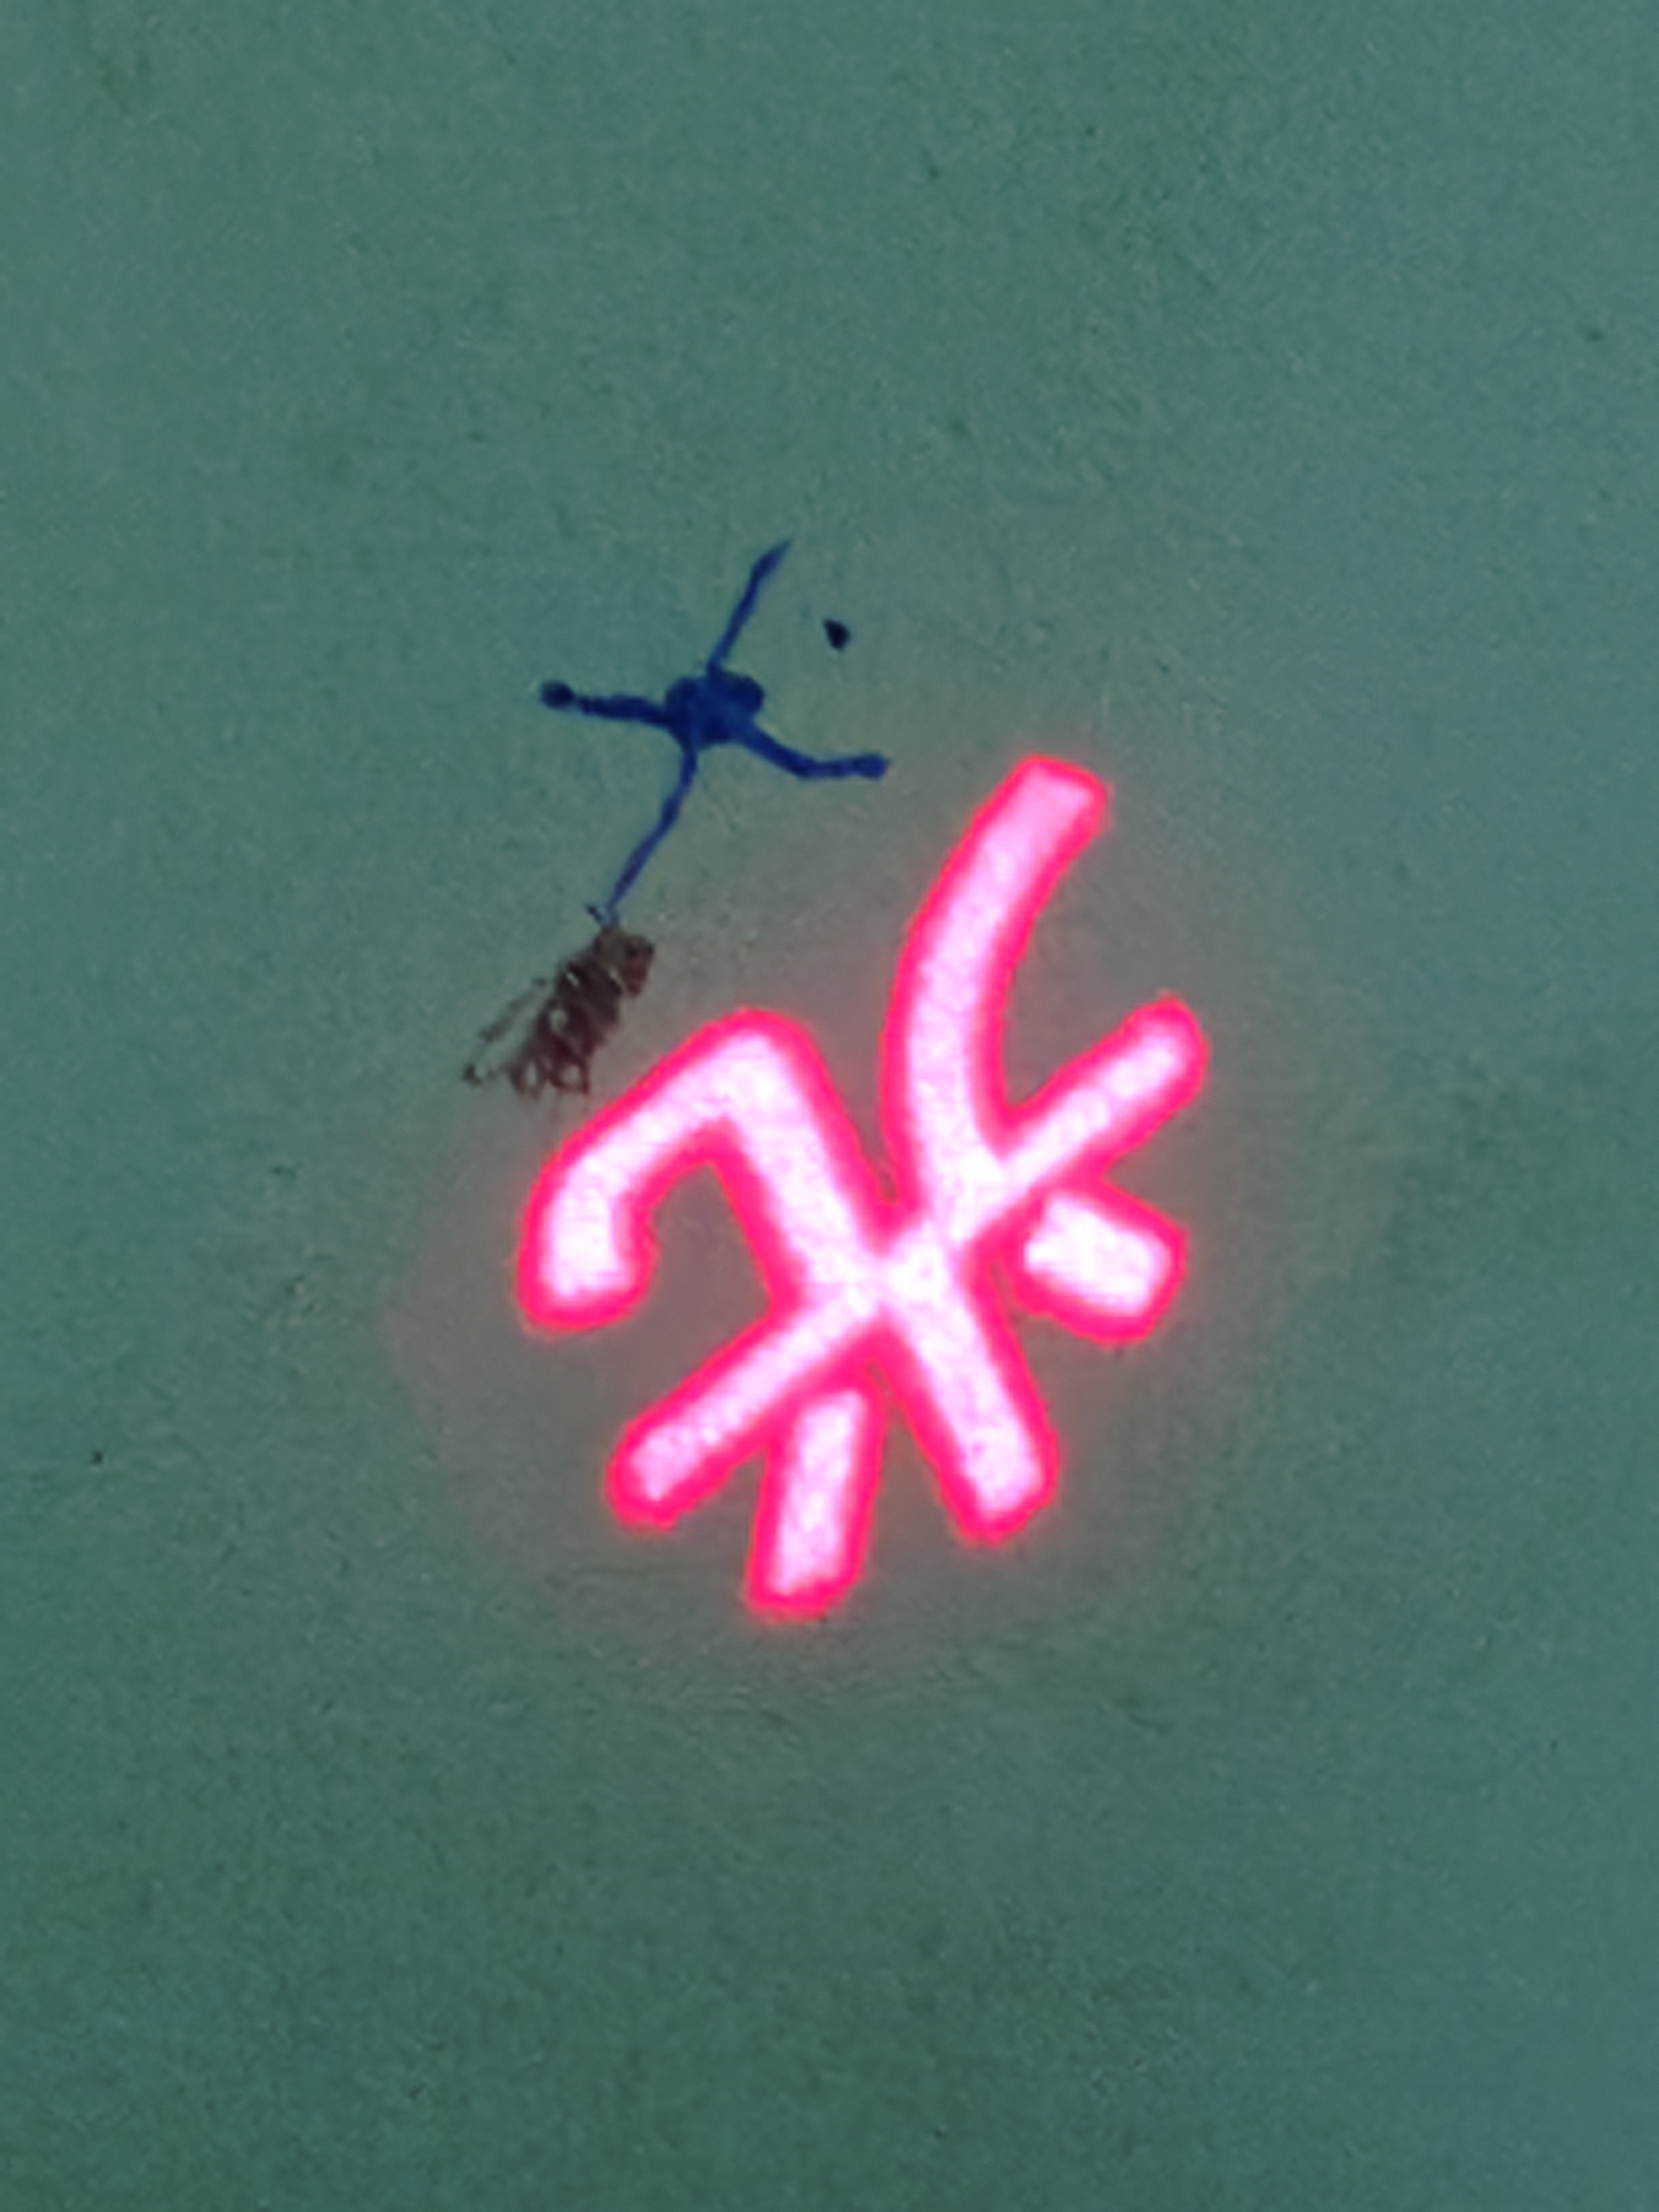
\includegraphics[width=0.3\textwidth]{fig21a.jpg}
    }
    \hspace{0.05\textwidth}
    \subfigure[成像图]{
        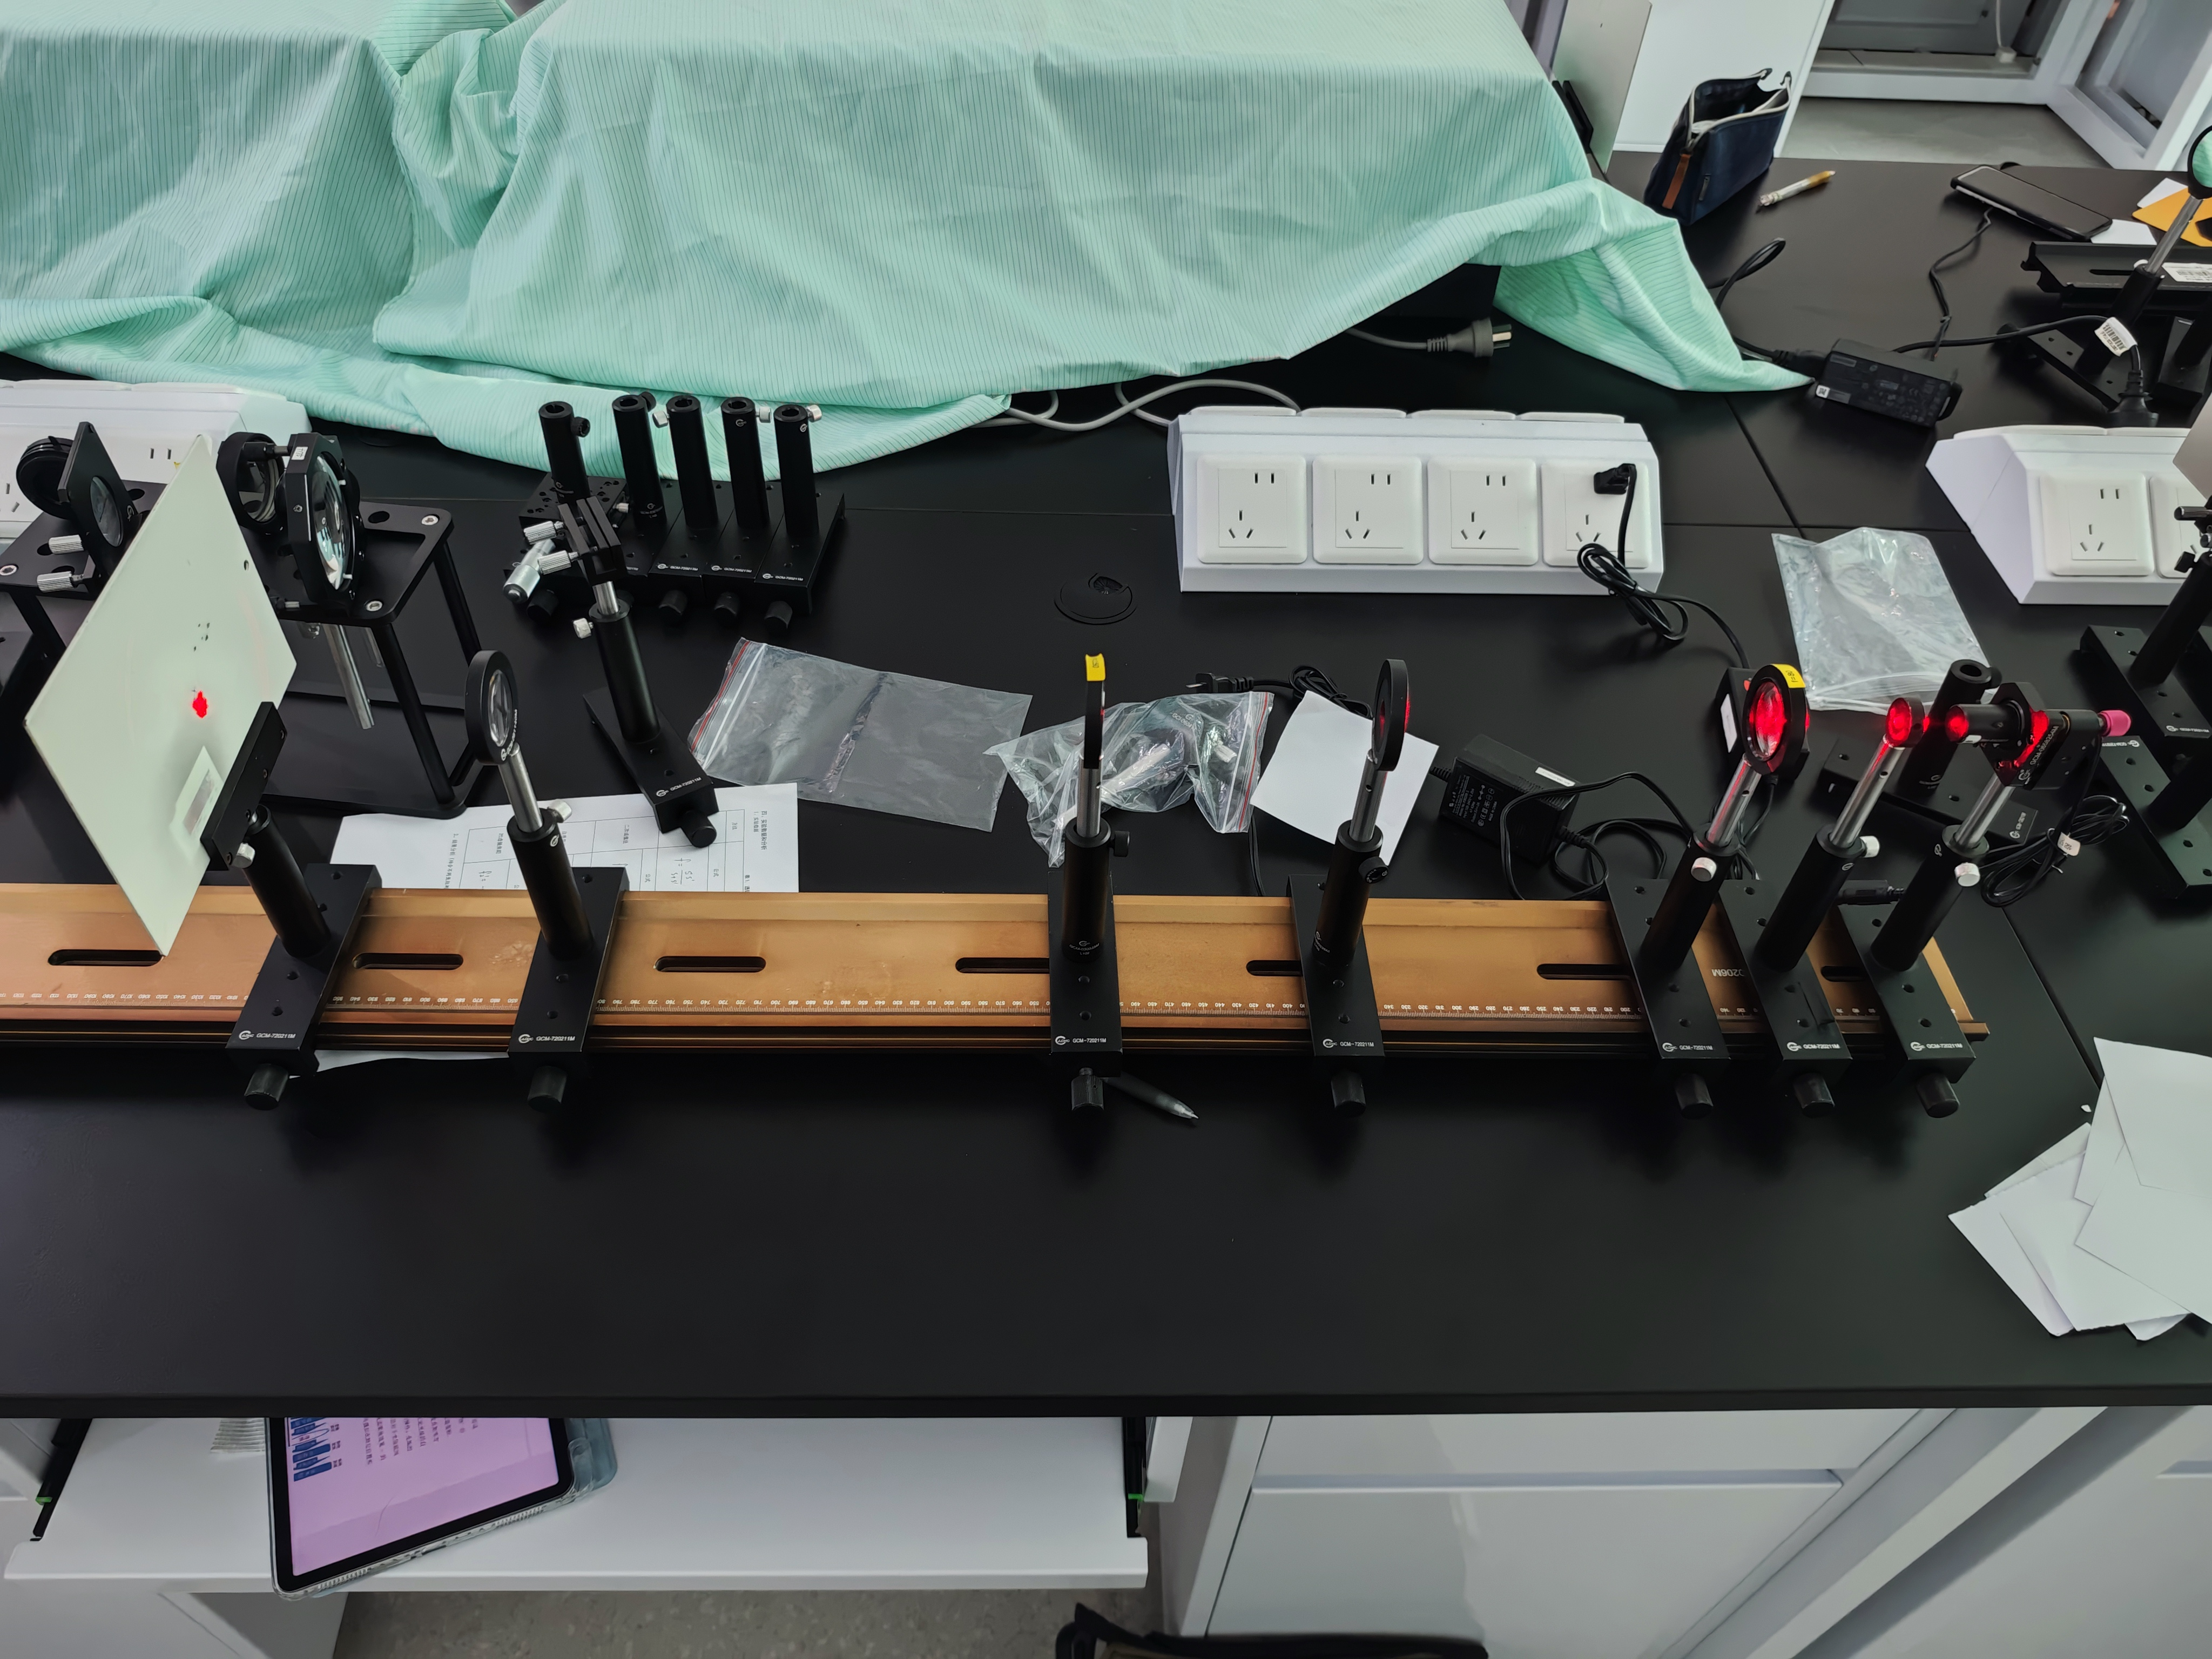
\includegraphics[width=0.3\textwidth]{fig21b.jpg}
    }
    \caption{光学4F系统成像结果1}
    \label{fig:fig21}
\end{figure}
\begin{figure}[!htbp]
    \centering
    \subfigure[光路图示]{
        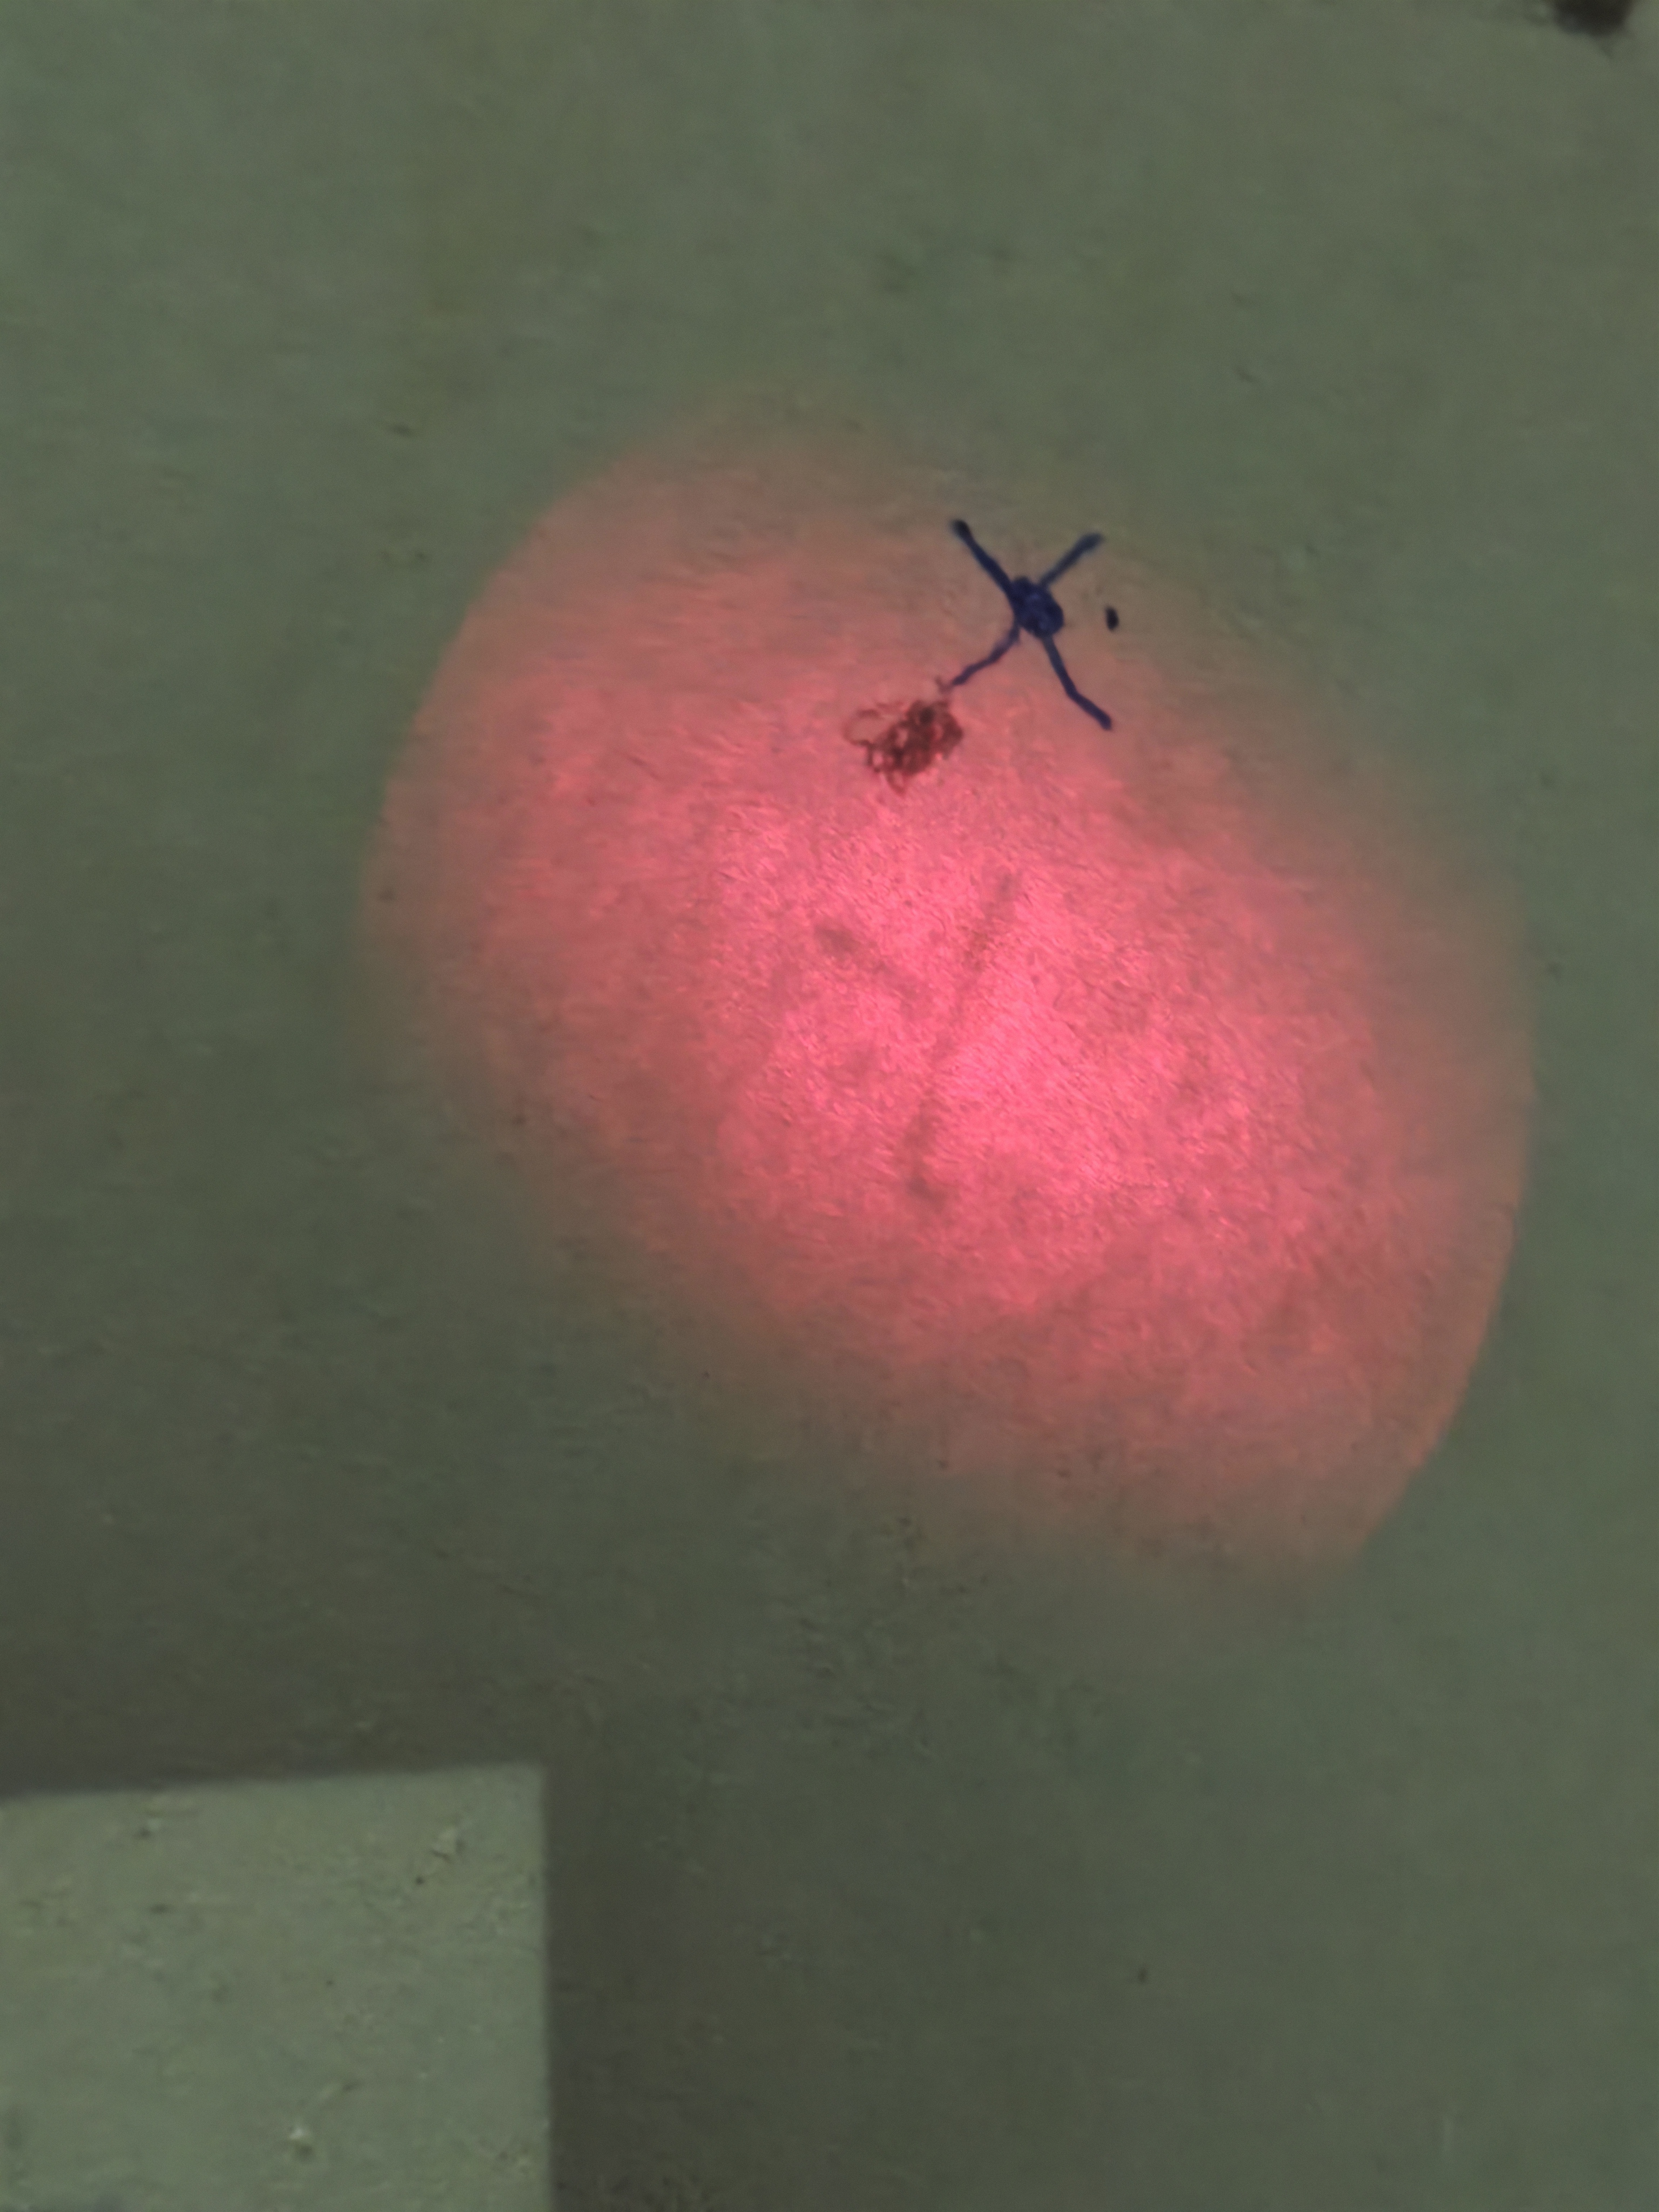
\includegraphics[width=0.3\textwidth]{fig22a.jpg}
    }
    \hspace{0.05\textwidth}
    \subfigure[成像图]{
        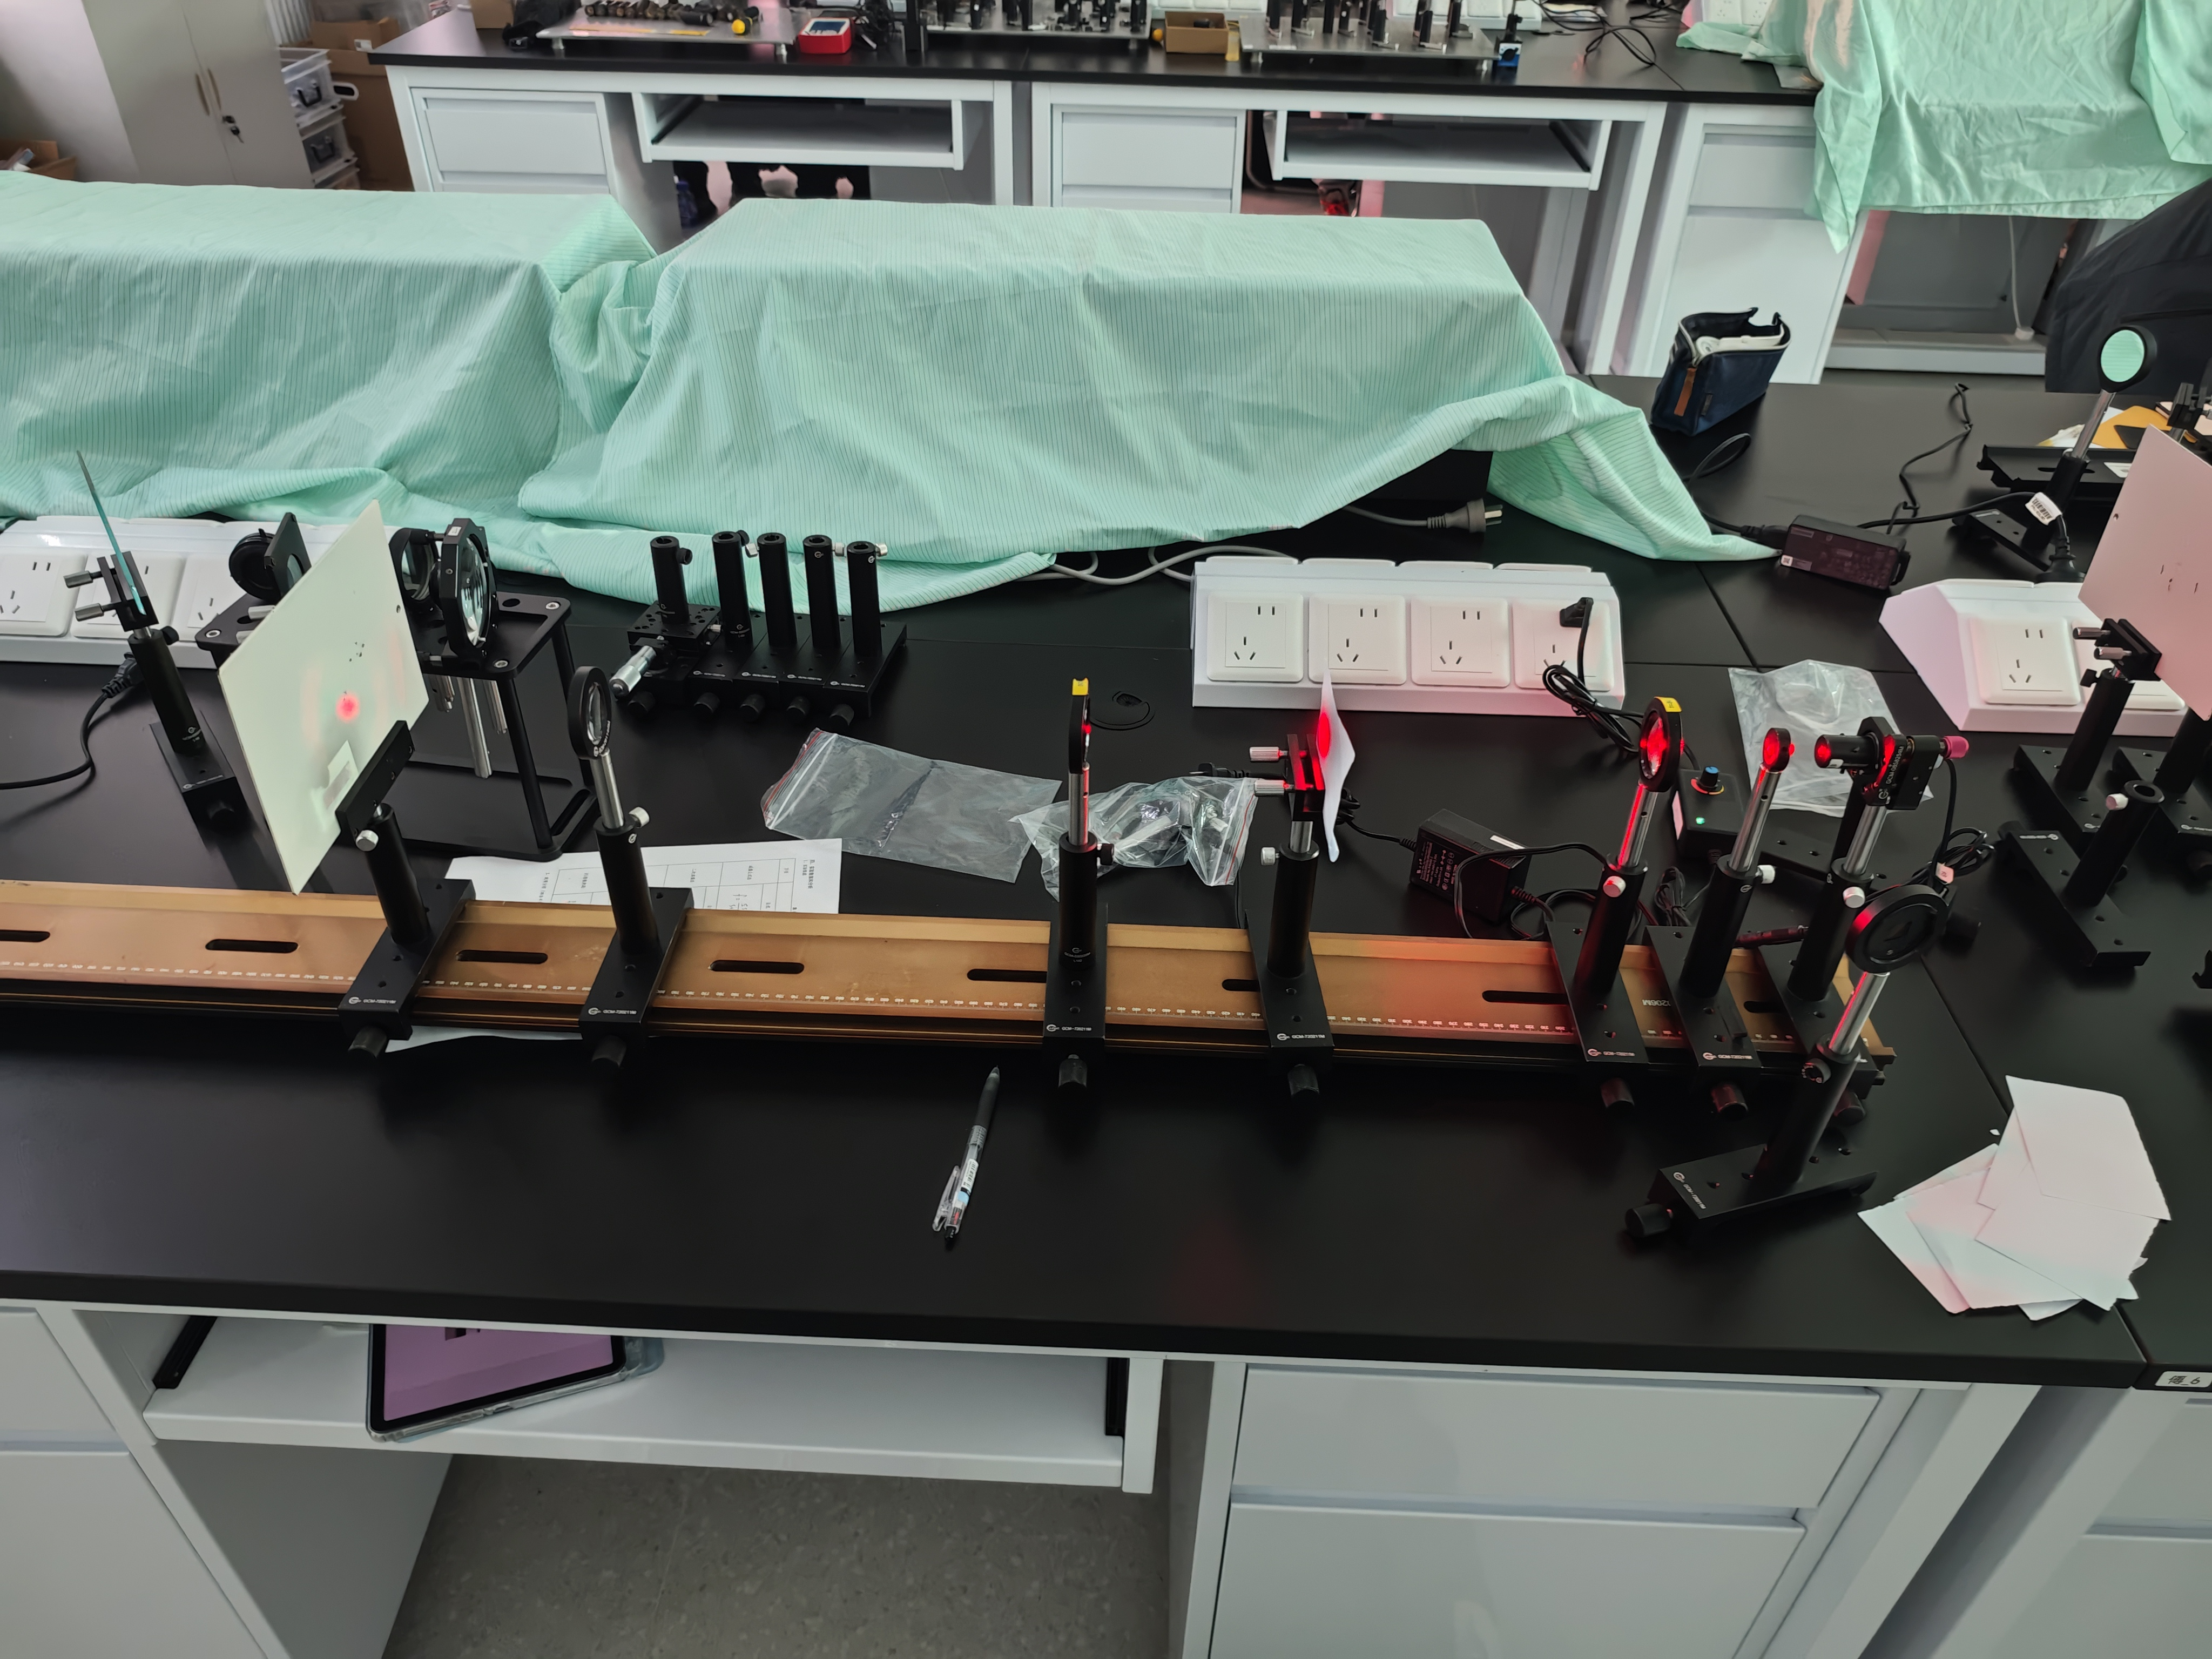
\includegraphics[width=0.3\textwidth]{fig22b.jpg}
    }
    \caption{光学4F系统成像结果2}
    \label{fig:fig22}
\end{figure}

\paragraph{结果分析与讨论}
通过对图\ref{fig:fig21}与图\ref{fig:fig22}的观察与测量，可以得出以下专业分析：
\begin{enumerate}
    \item \textbf{成像保真度与放大率验证}：实验结果显示，像面形成了与物孔尺寸严格 1:1 对应的倒立实像。这验证了当两透镜焦距相等（$f_1 = f_2$）时，4F 系统的横向放大率 $M = -f_2/f_1 = -1$。图像边缘锐利，畸变极小，证明了系统共轴调节的精确性。
    \item \textbf{复振幅传递与相位保真}：与单透镜成像系统不同，4F 系统通过两次傅里叶变换的级联，在像平面上消除了单透镜成像中固有的二次相位因子 $\exp[i\frac{k}{2d_i}(x^2+y^2)]$。这意味着该系统不仅实现了强度的 1:1 传递，更实现了复振幅分布的精确复制，这对于相干光学处理（如全息术或复数滤波器应用）至关重要。
    \item \textbf{频谱面处理的解耦性}：在实验过程中，通过在两透镜间的共焦面（频谱面）放置滤波器，可以观察到像面特征的即时改变。这体现了 4F 系统最核心的优势：将傅里叶变换功能与成像功能在空间上完全解耦。这种结构允许我们在不改变成像几何参数的前提下，通过对频谱面进行精细操作（如低通、高通或方向滤波）来调控最终的成像质量。
    \item \textbf{像差抑制分析}：实验中遵循“凹凸面对准平行光”的原则对称放置透镜，有效地抑制了球差和彗差。观察到的像面亮度均匀，对比度高，说明系统对高频分量的截断效应较小，保持了较高的空间分辨率。
\end{enumerate}

\subsection{θ调制假彩色编码结果}
\begin{figure}[!htbp]
    \centering
    \subfigure[光路图示]{
        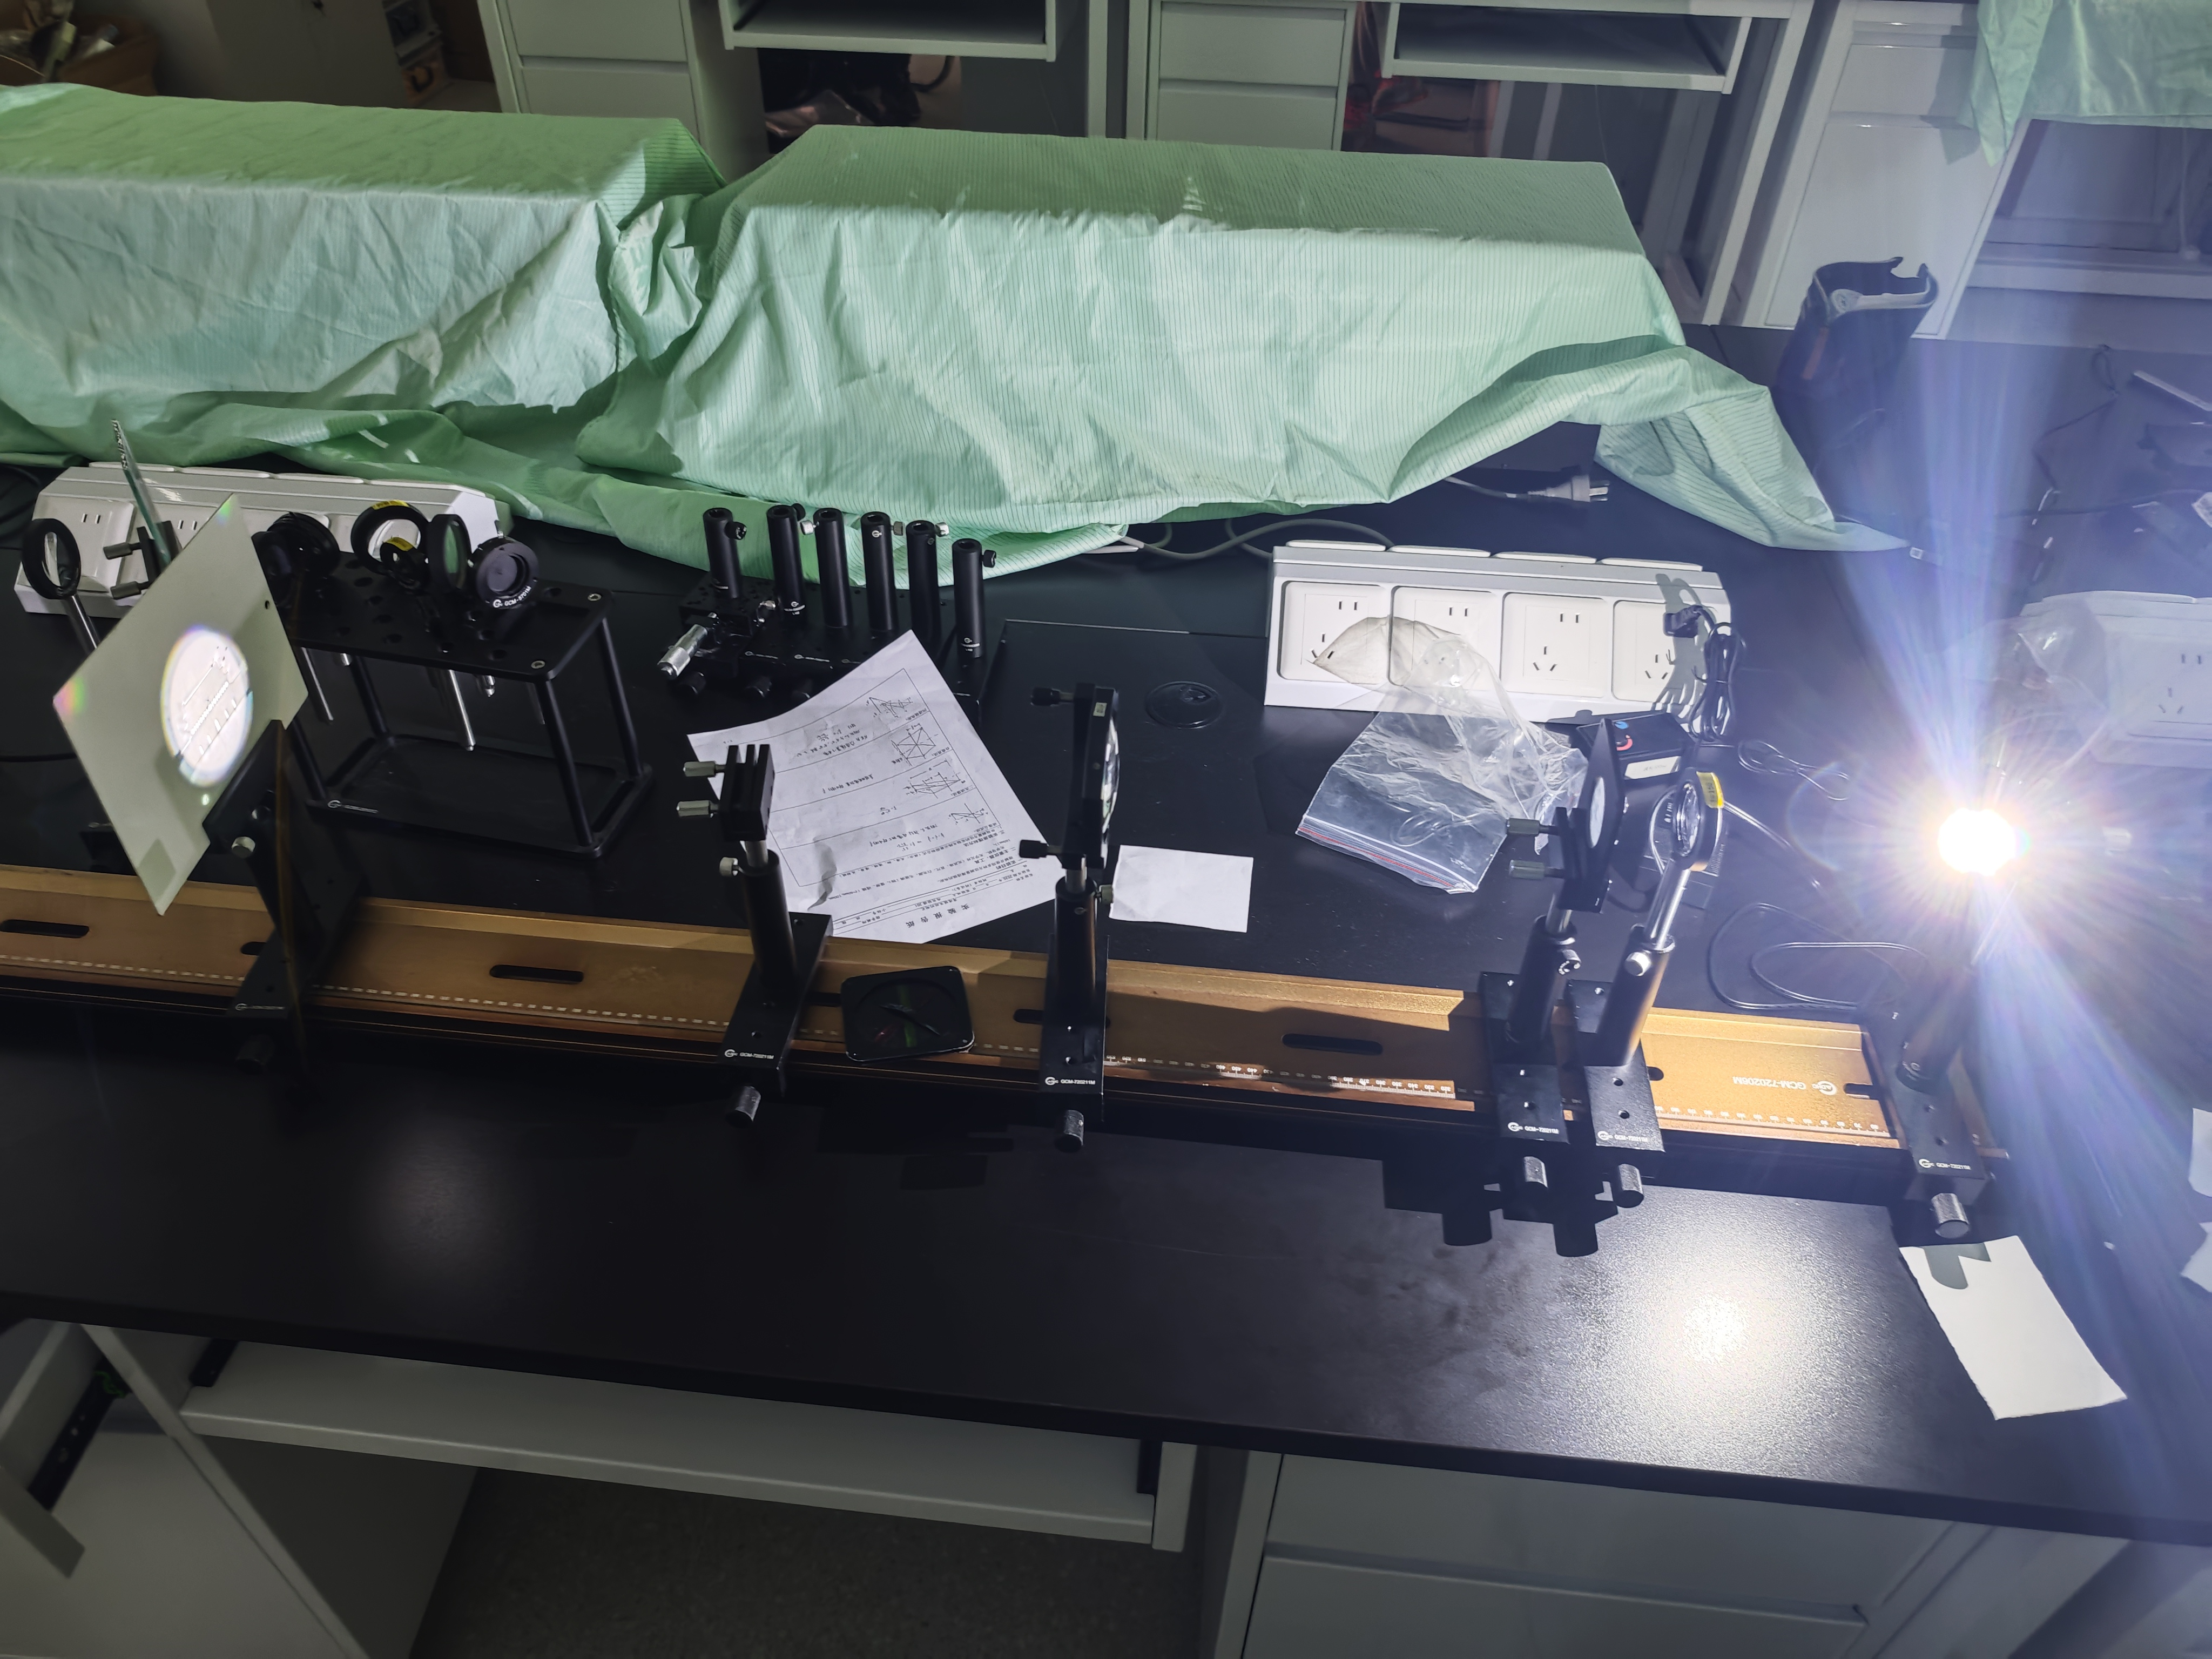
\includegraphics[width=0.3\textwidth]{IMG_20251105_161132.jpg}
    }
    \hspace{0.05\textwidth}
    \subfigure[成像图]{
        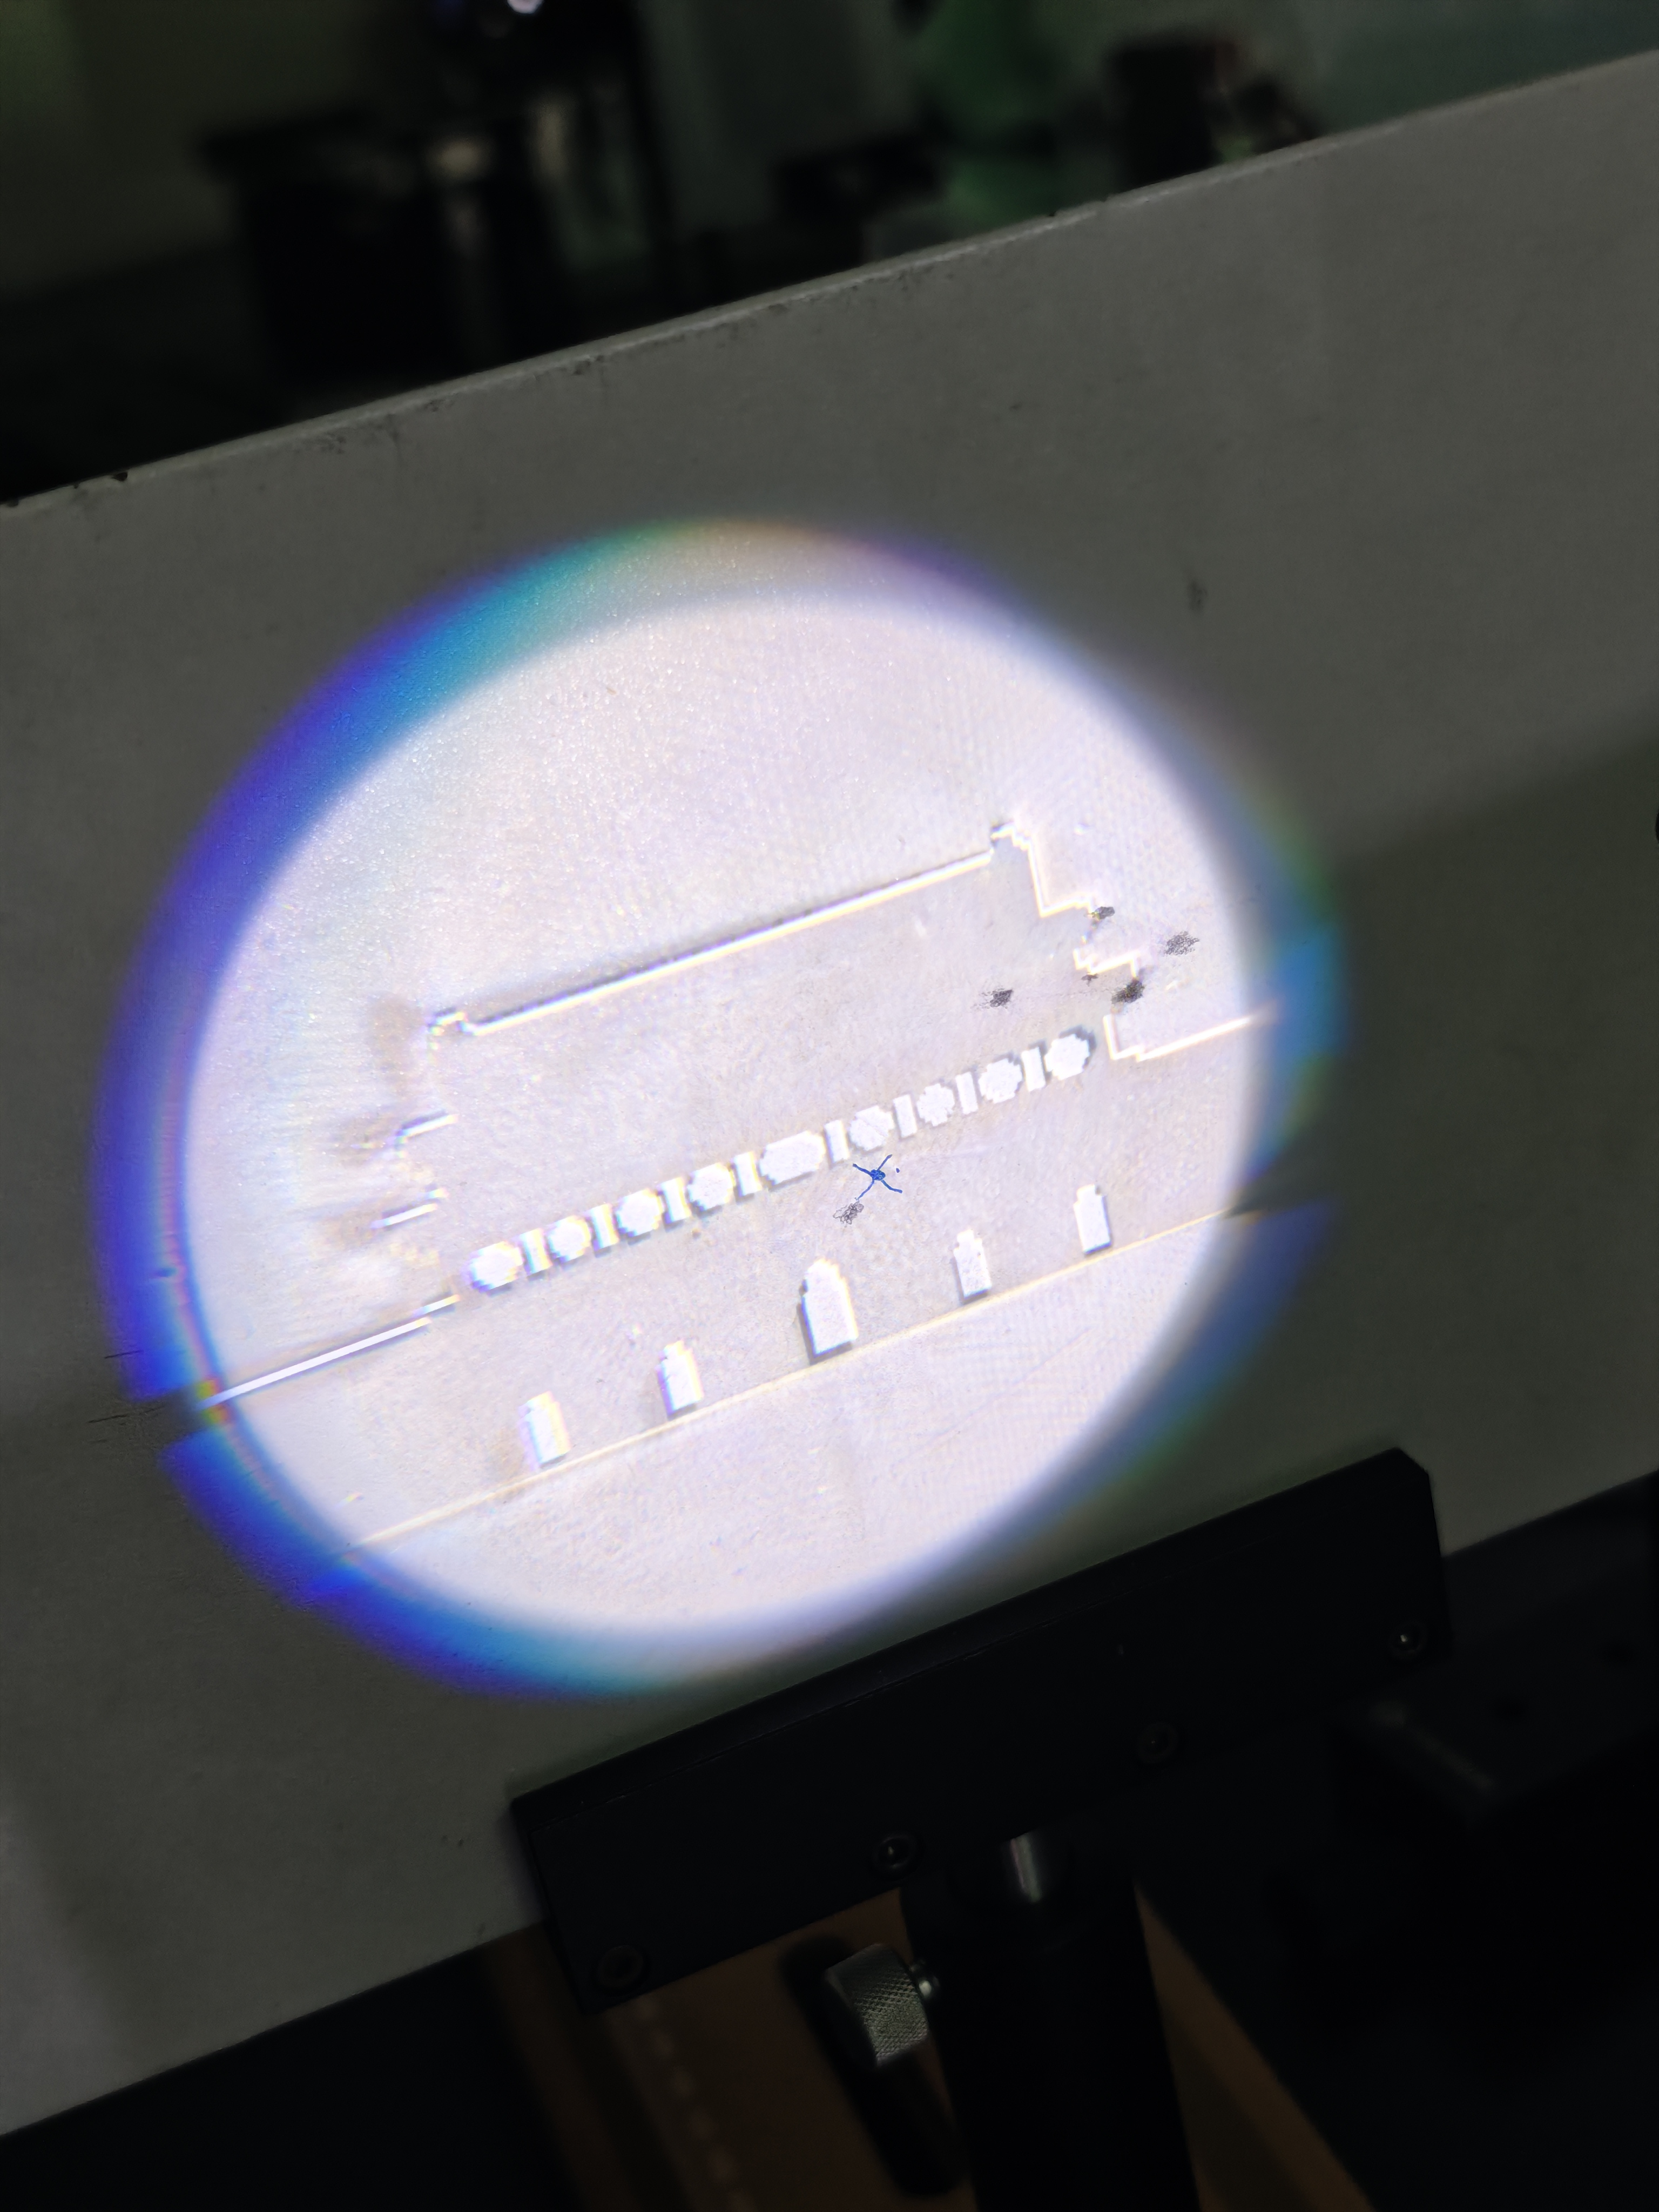
\includegraphics[width=0.3\textwidth]{IMG_20251105_161358.jpg}
    }
    \caption{θ调制假彩色编码结果1}
\end{figure}
\paragraph{不加滤波器时}像面显示出模糊的黑白“天安门”图案，缺乏颜色信息。
\begin{figure}[!htbp]
    \centering
    \subfigure[光路图示]{
        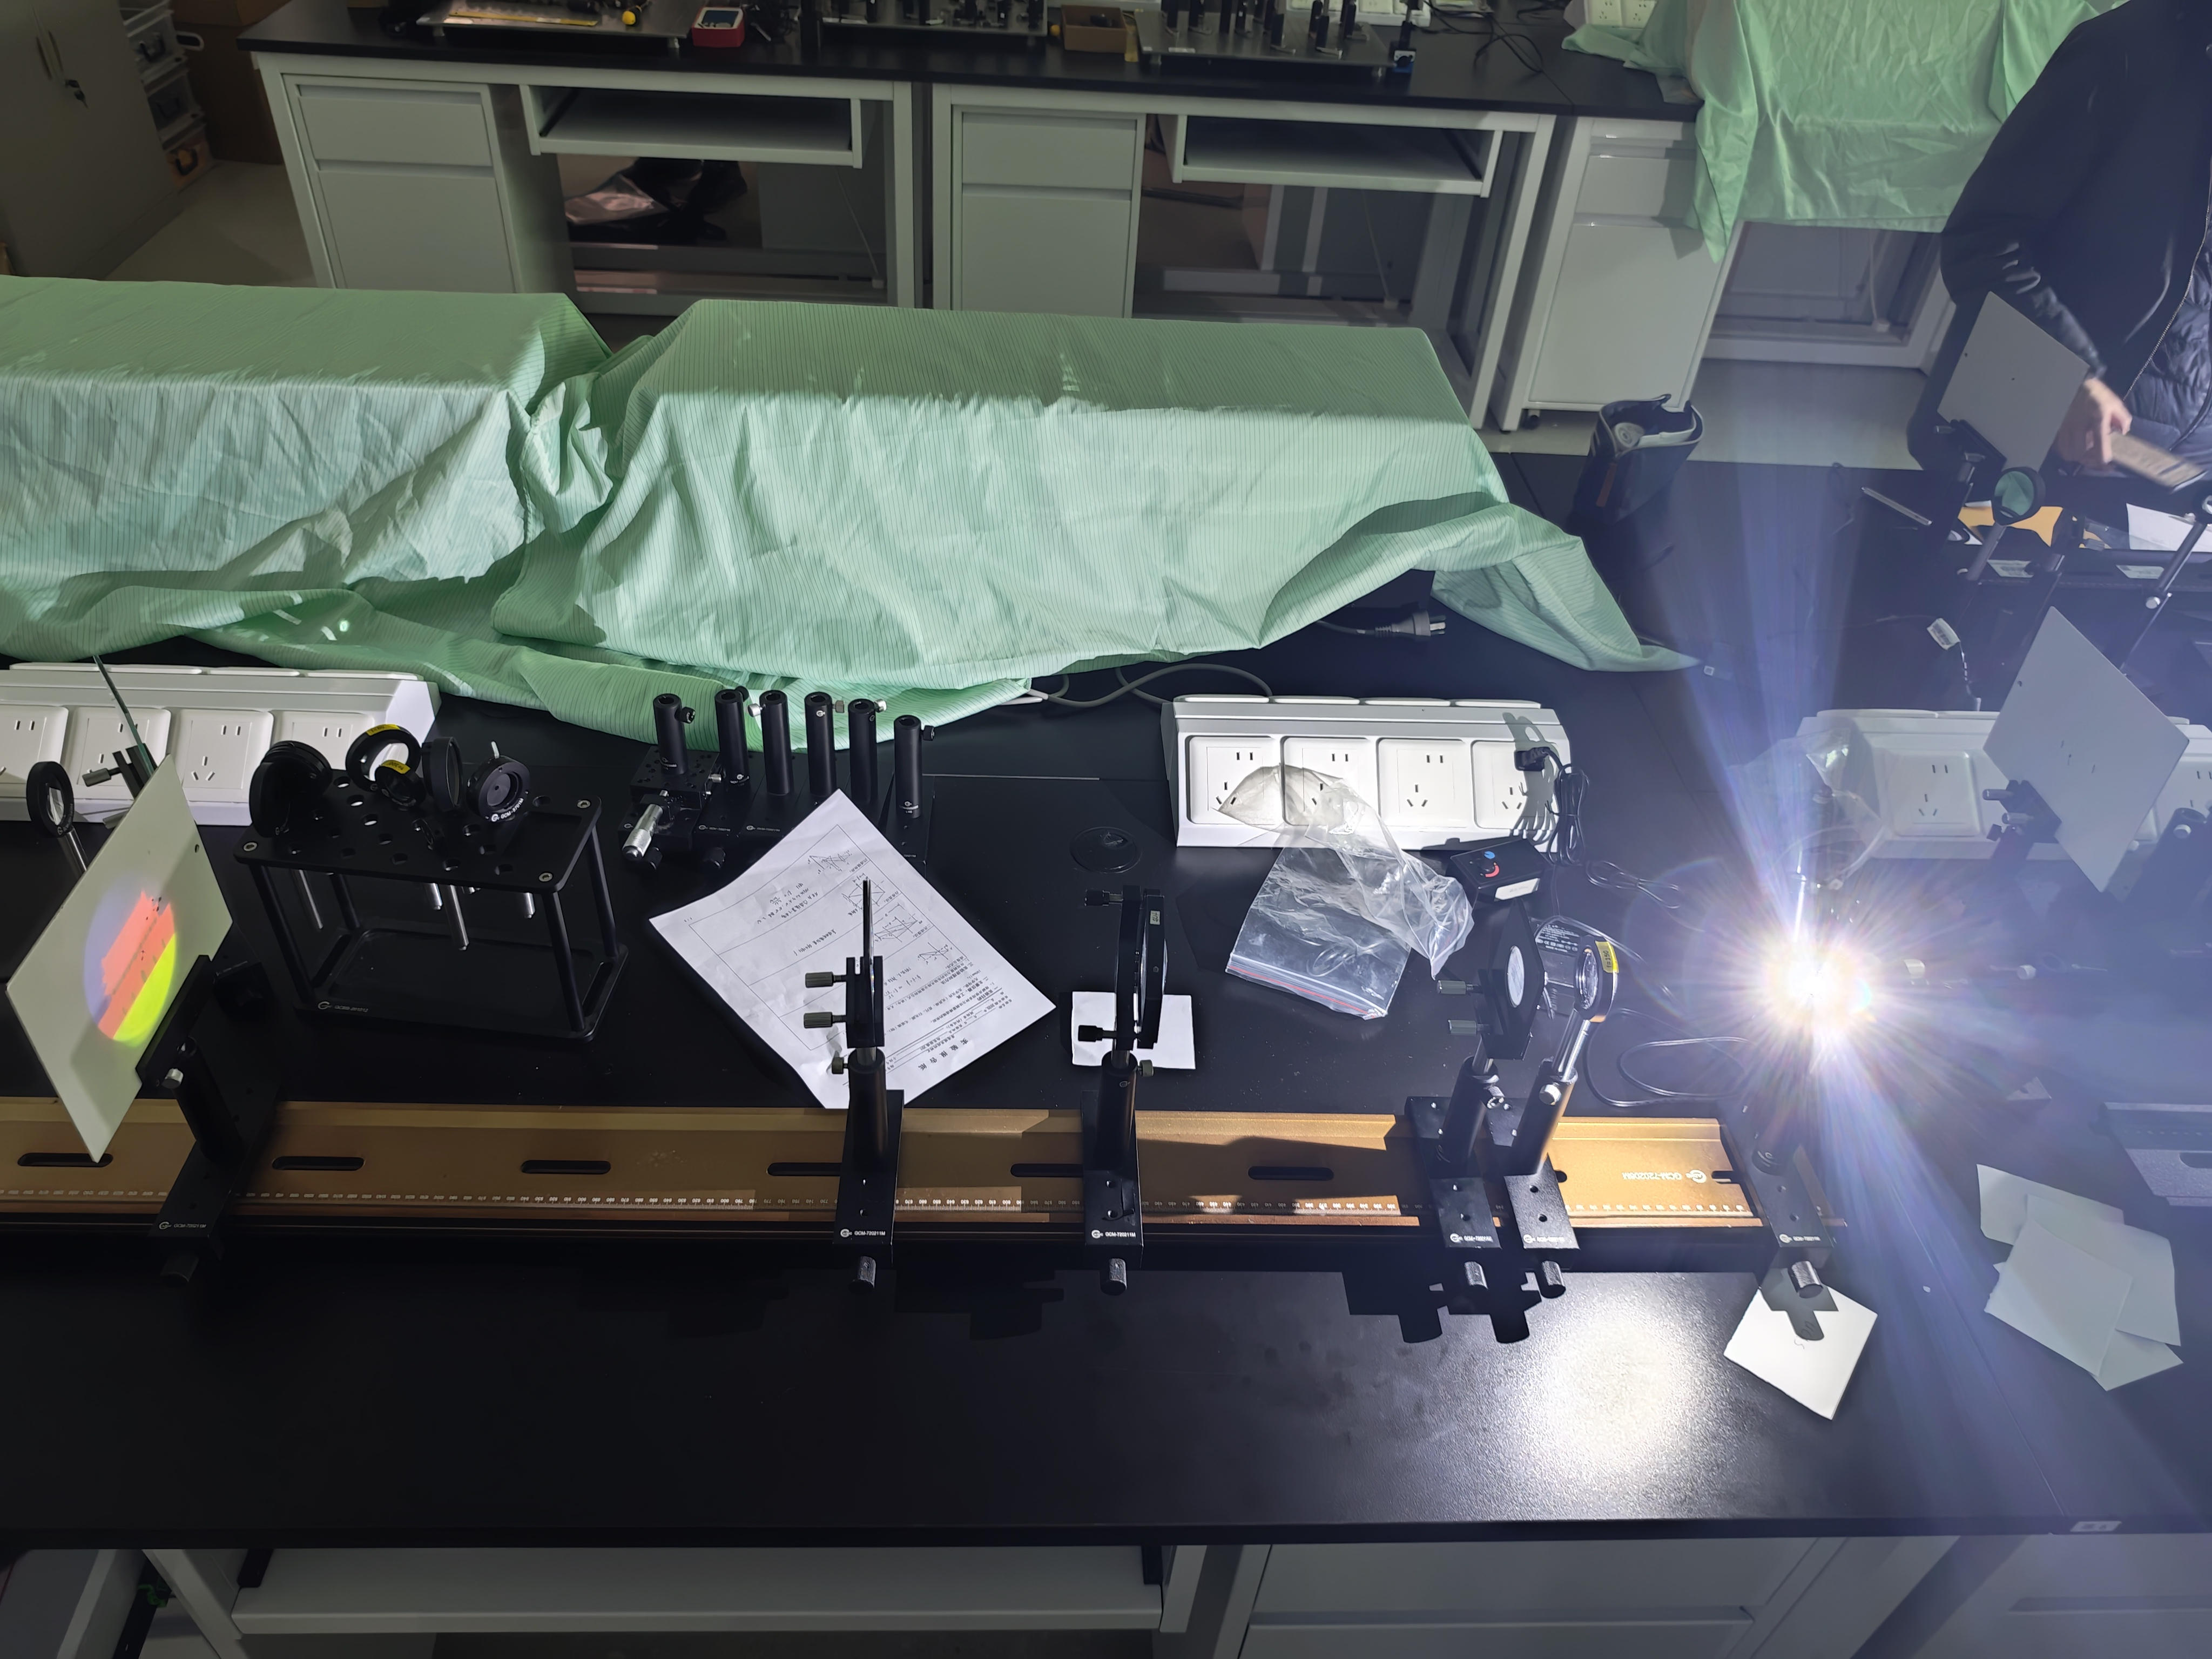
\includegraphics[width=0.2\textwidth]{fig23b.jpg}
    }
    \hspace{0.05\textwidth}
    \subfigure[成像图]{
        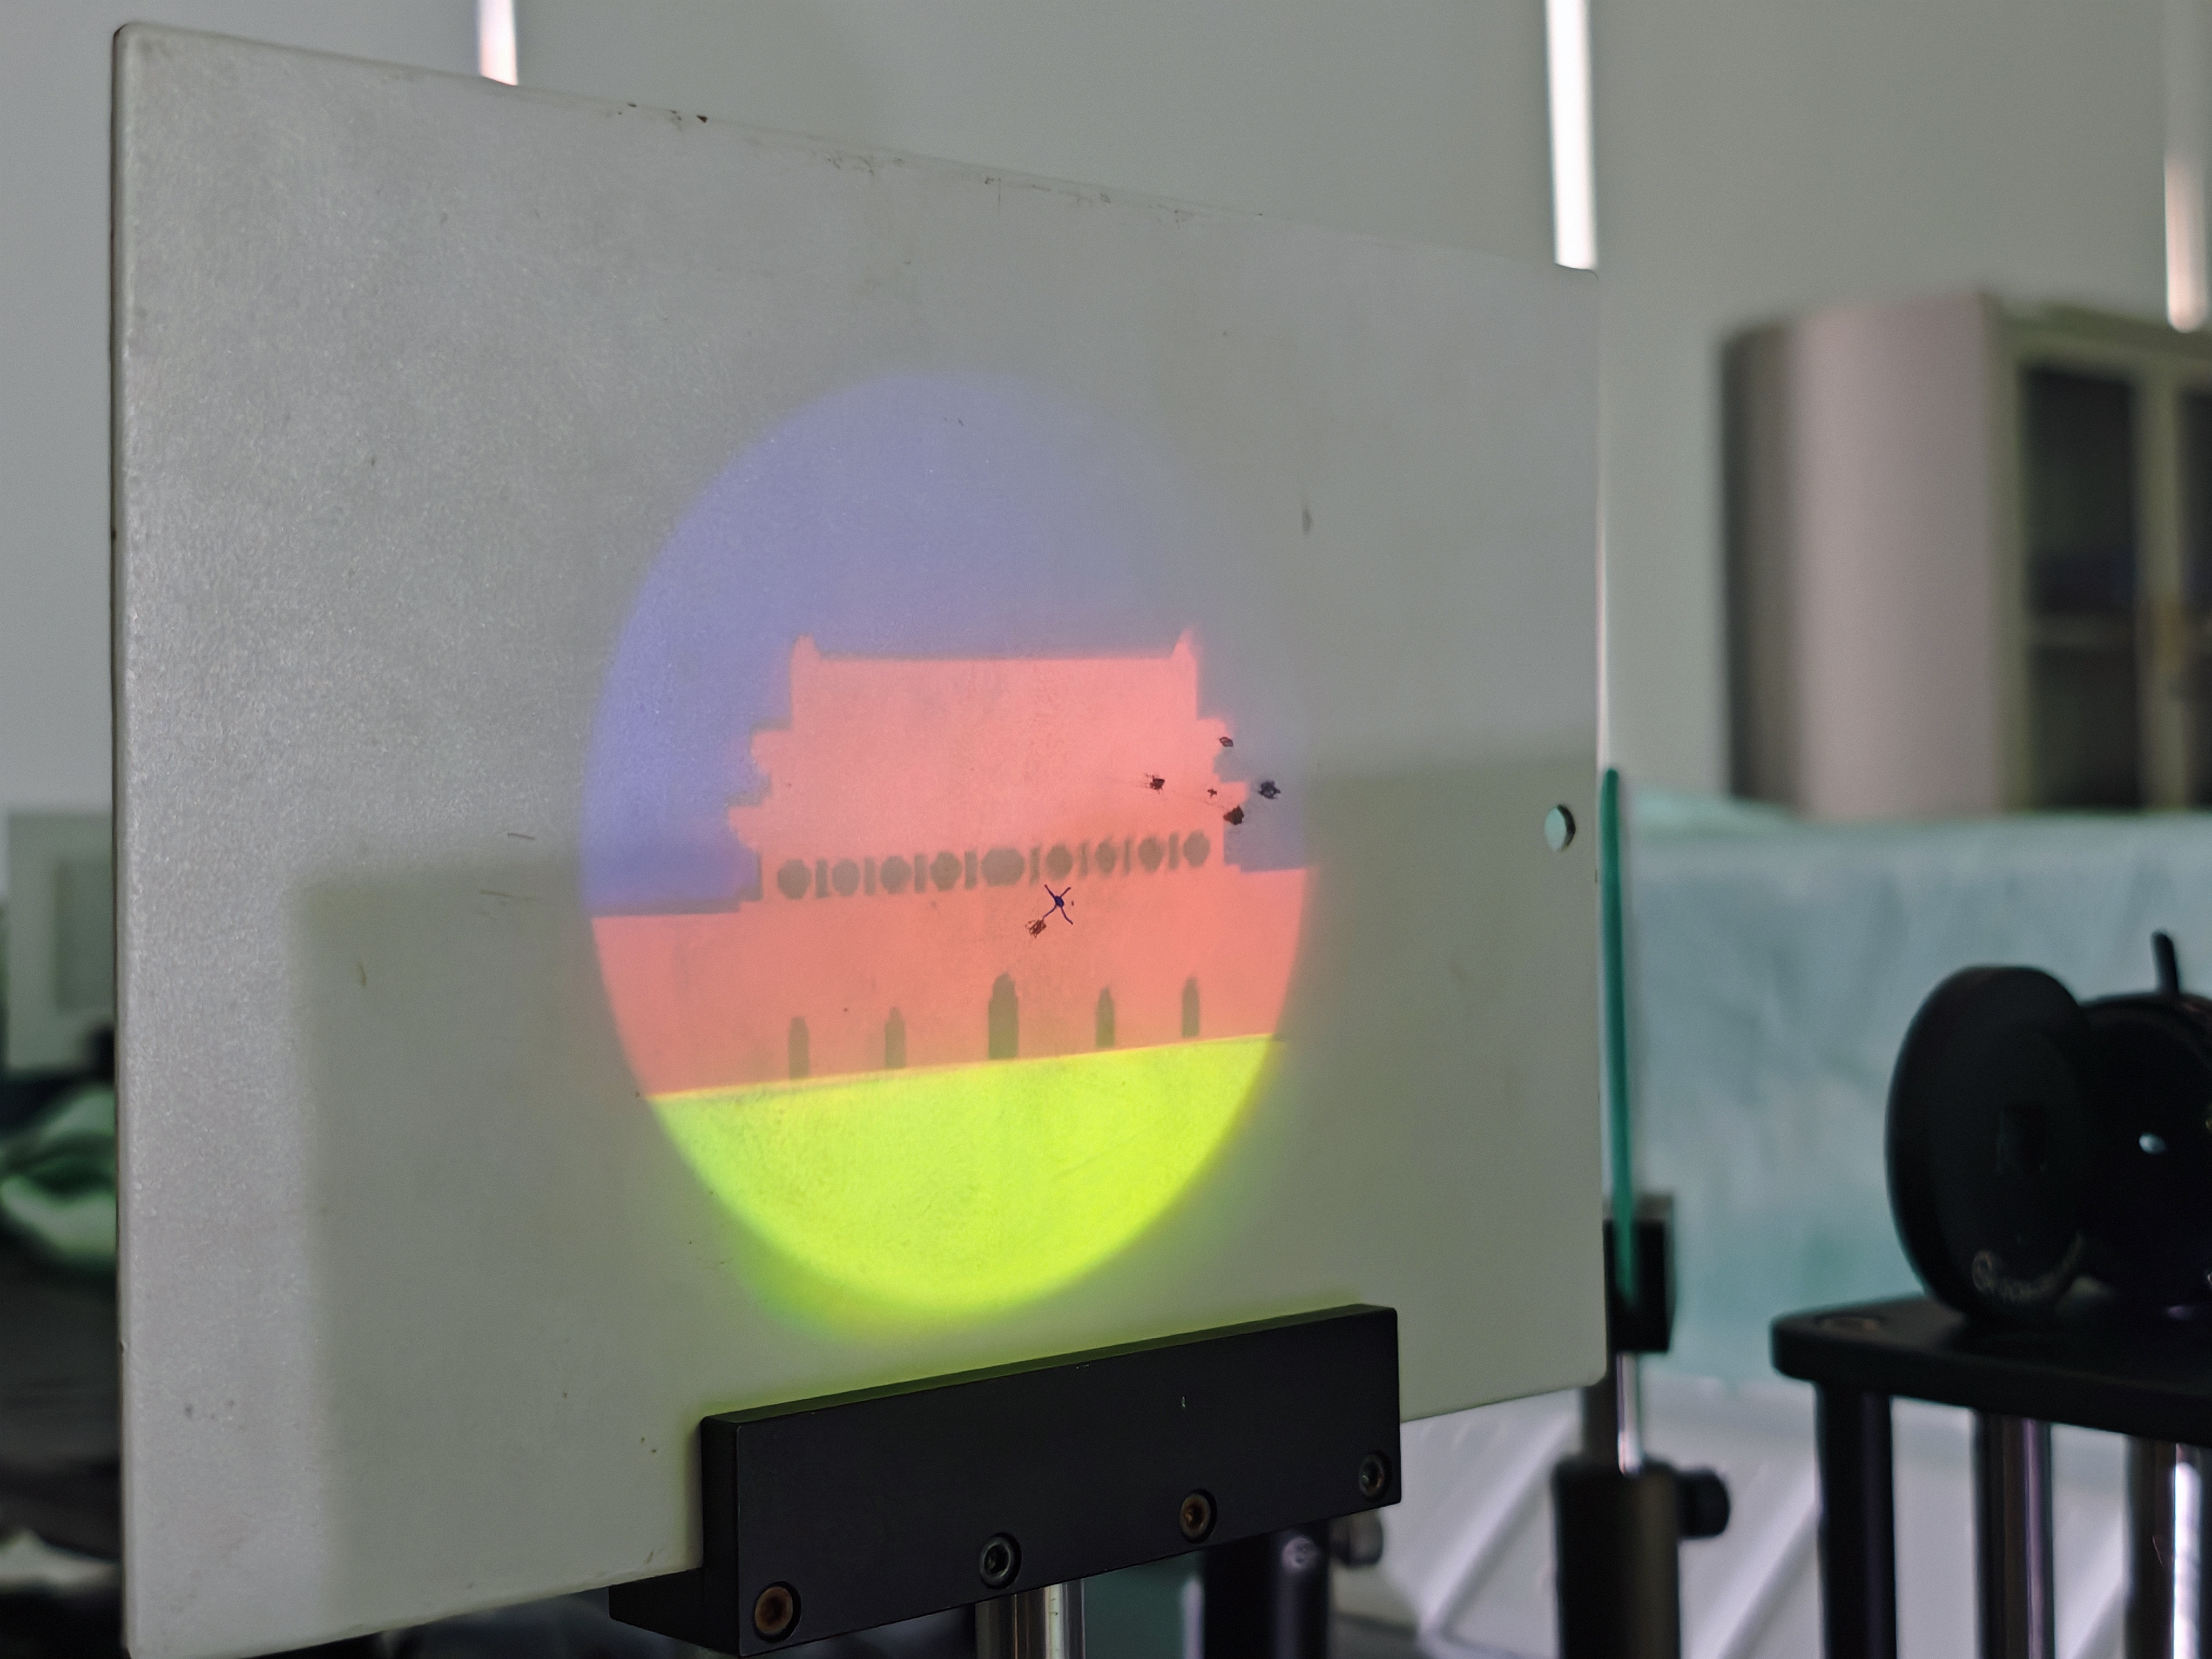
\includegraphics[width=0.2\textwidth]{fig23a.jpg}
    }
    \subfigure[频谱面图像]{
        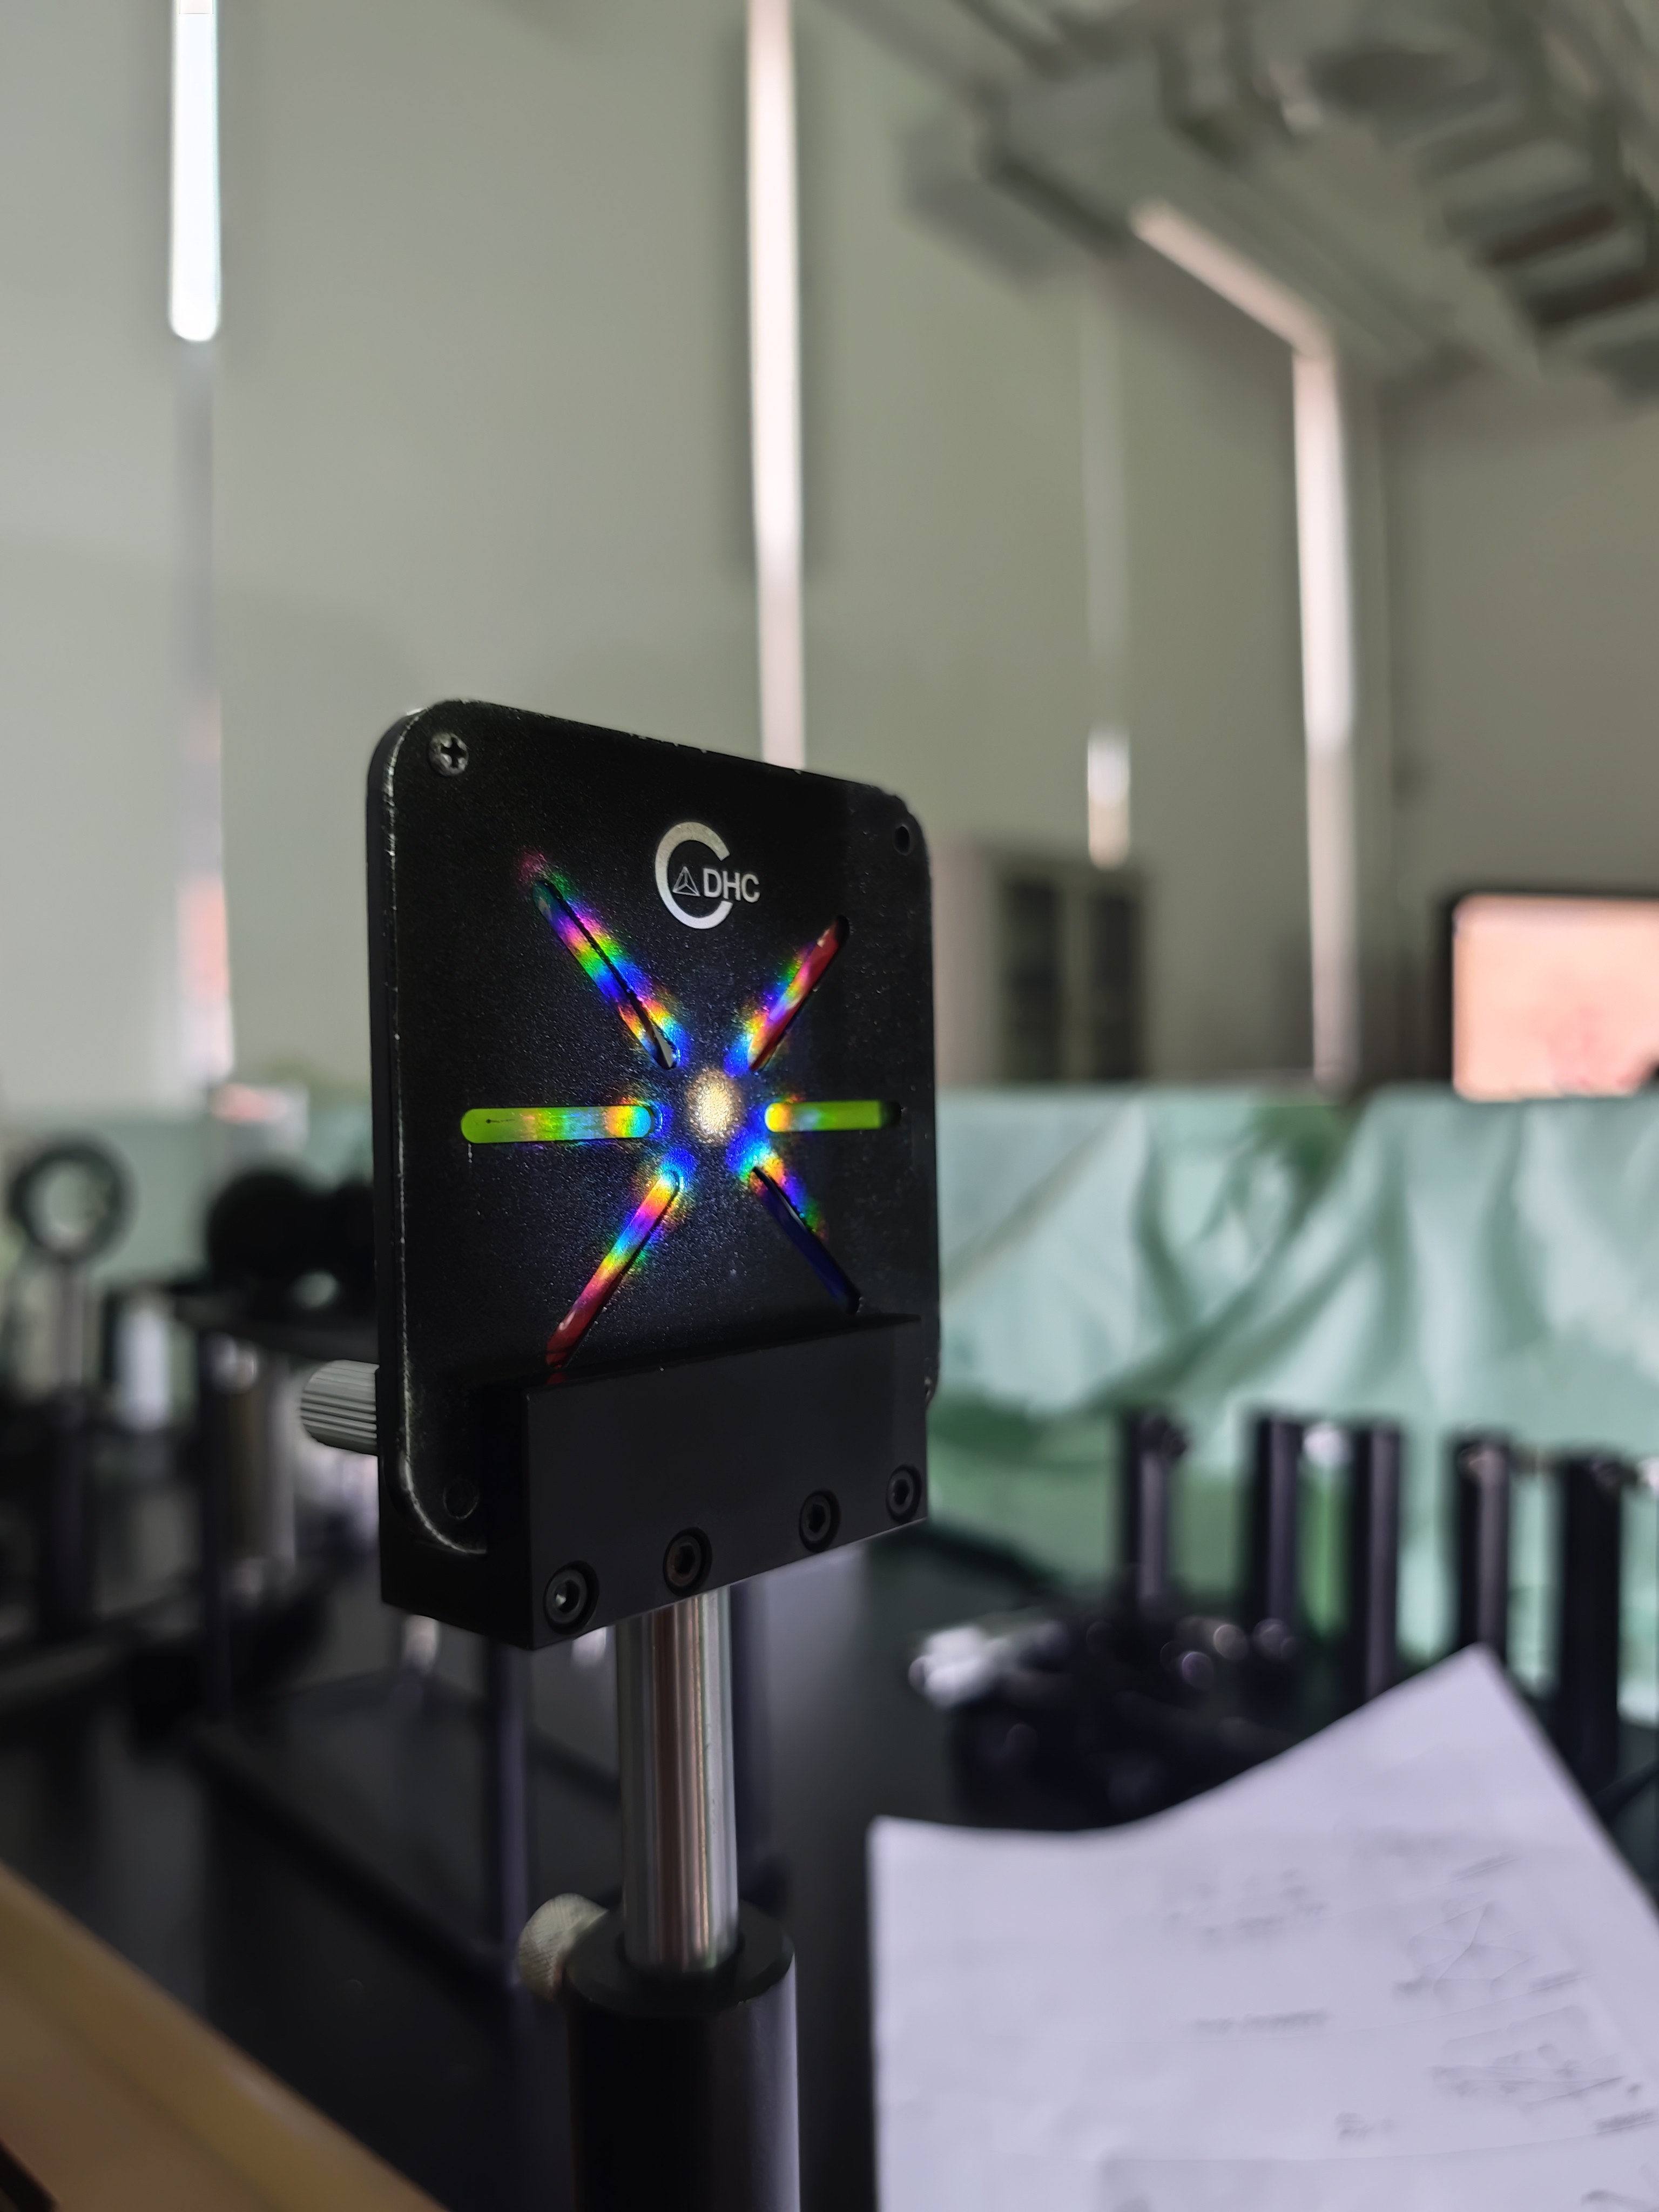
\includegraphics[width=0.2\textwidth]{fig23c.jpg}
    }
    \subfigure[成像图2]{
        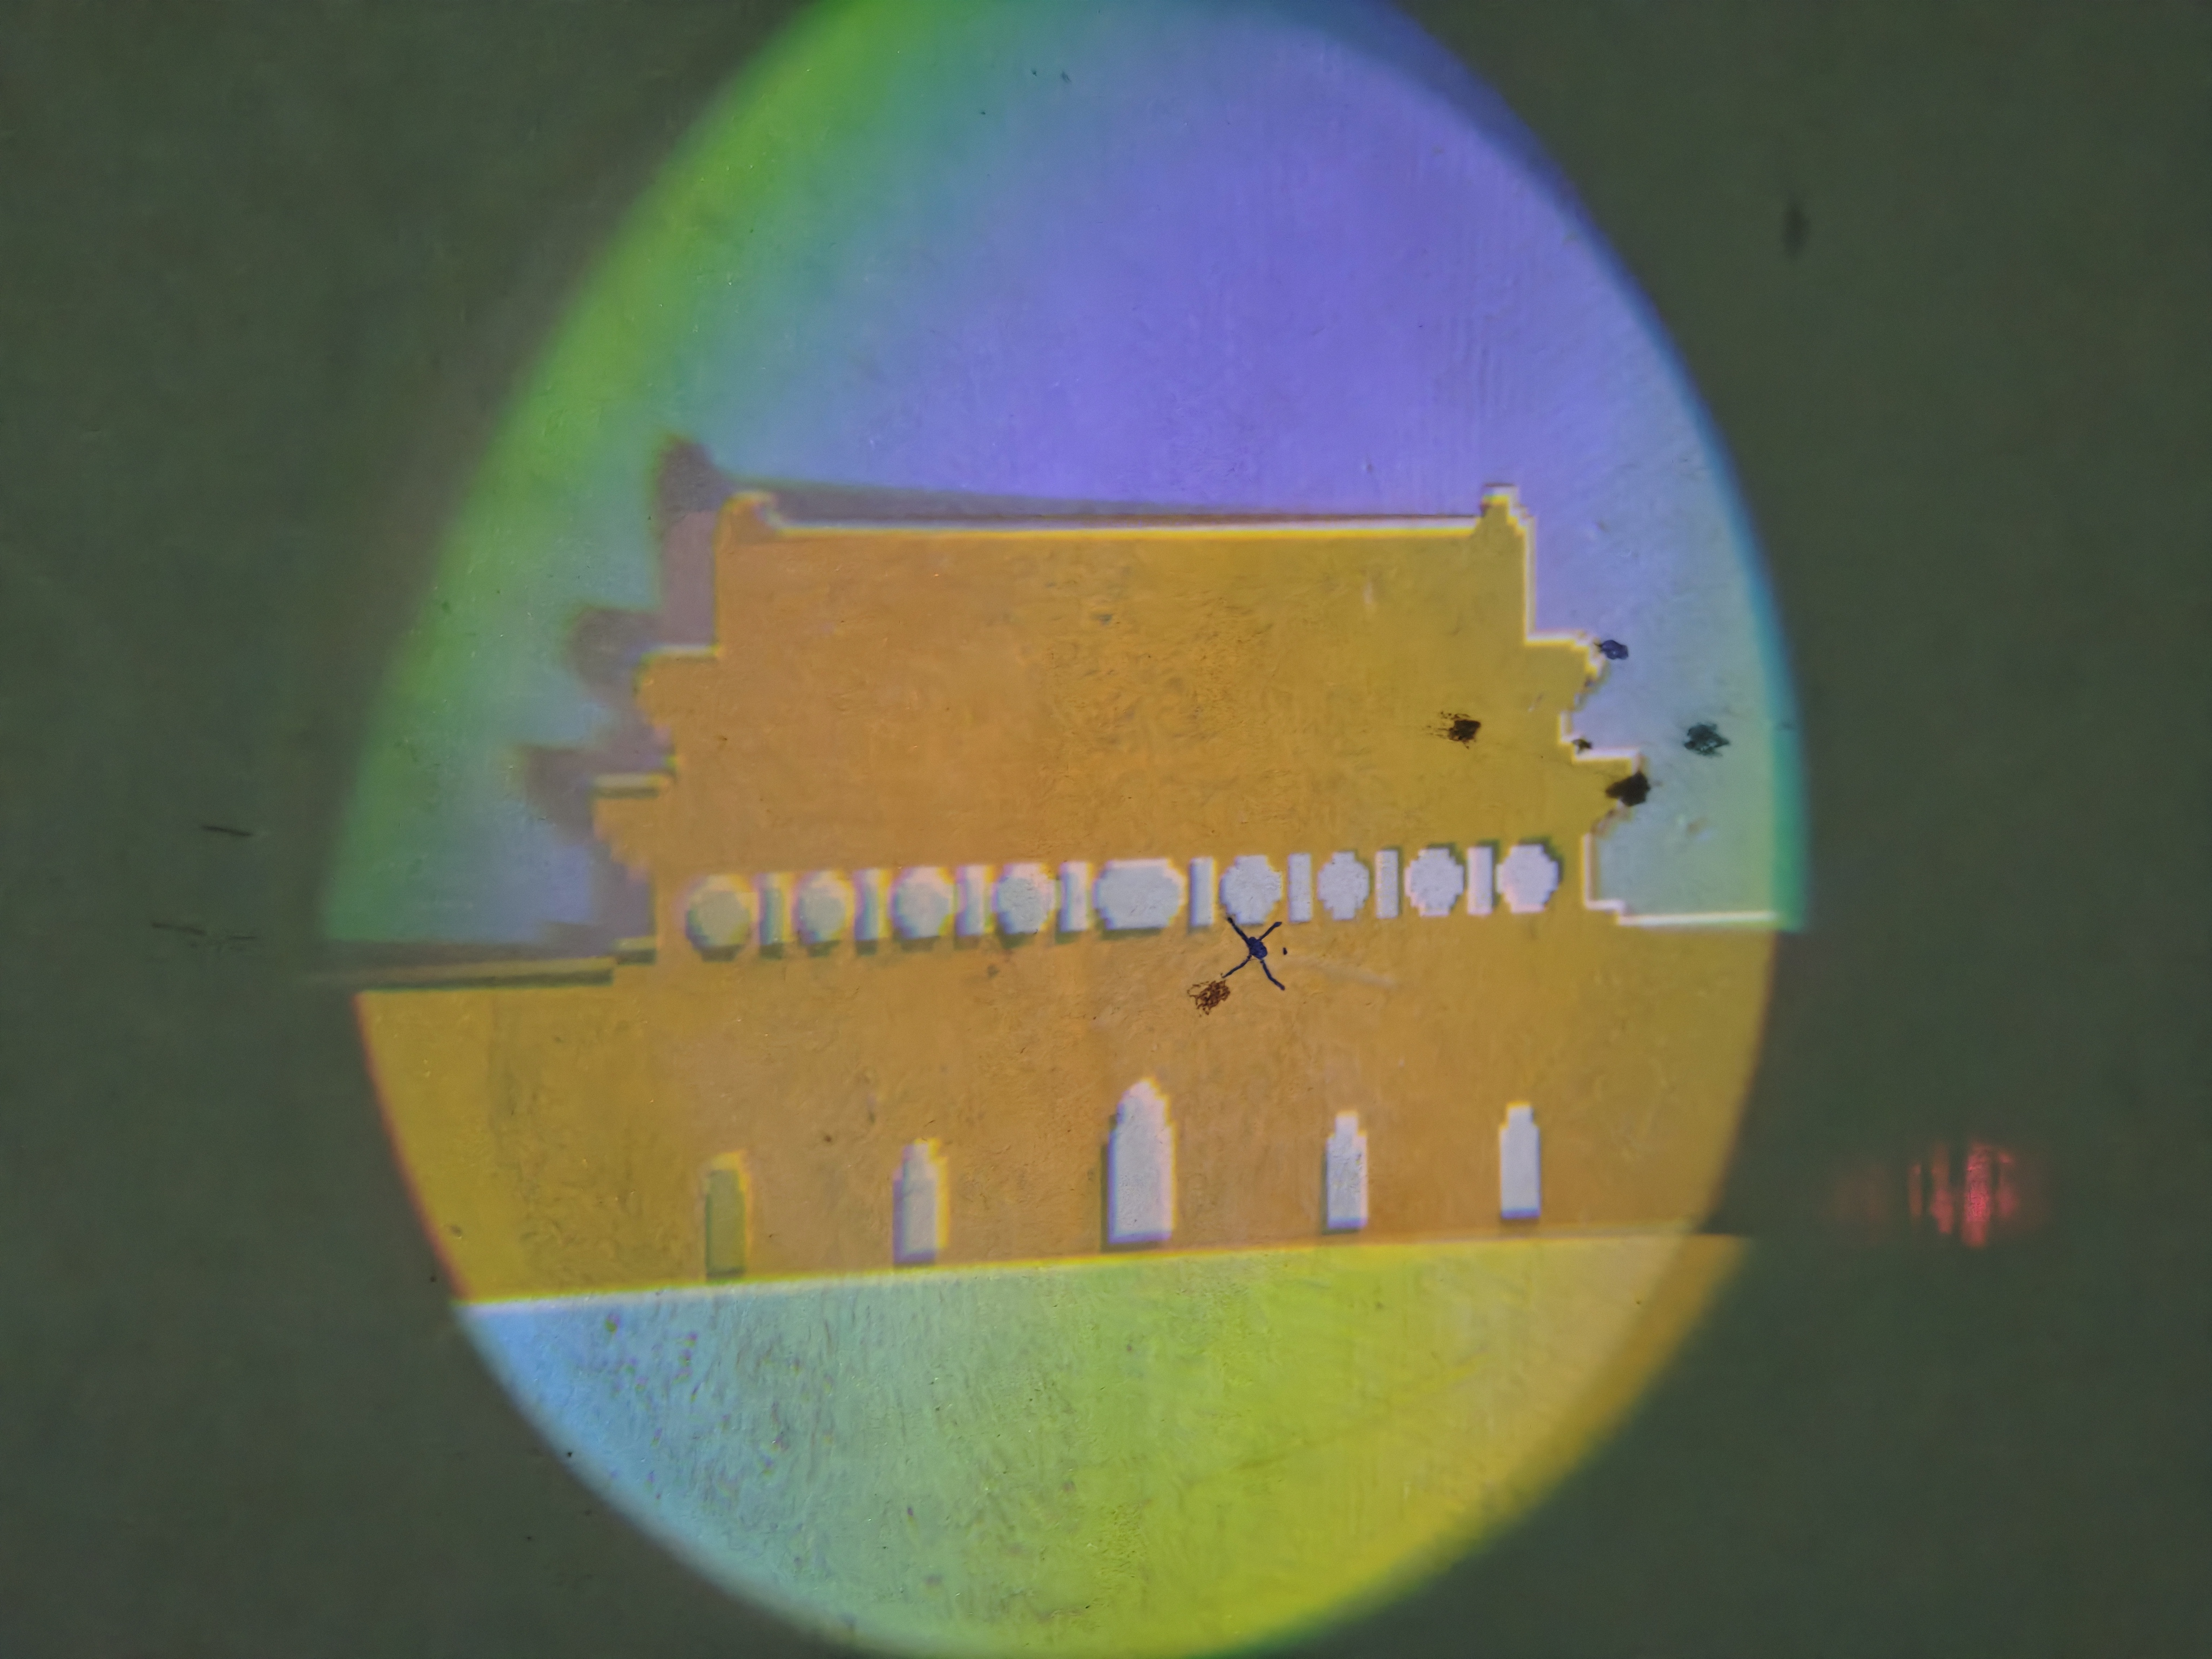
\includegraphics[width=0.2\textwidth]{fig23d.jpg}
    }
    \caption{θ调制假彩色编码结果2}
\end{figure}
\paragraph{加滤波器时}通过调整θ调制滤波器位置，实现了“天安门”图案的假彩色显示：天空呈现蓝色，城楼为红色，草地为绿色，验证了θ调制空间编码原理。将中间的孔变为透光时可以让天安门城楼中的窗户亮起
\begin{figure}[!htbp]
    \centering
    \subfigure[光路图示]{
        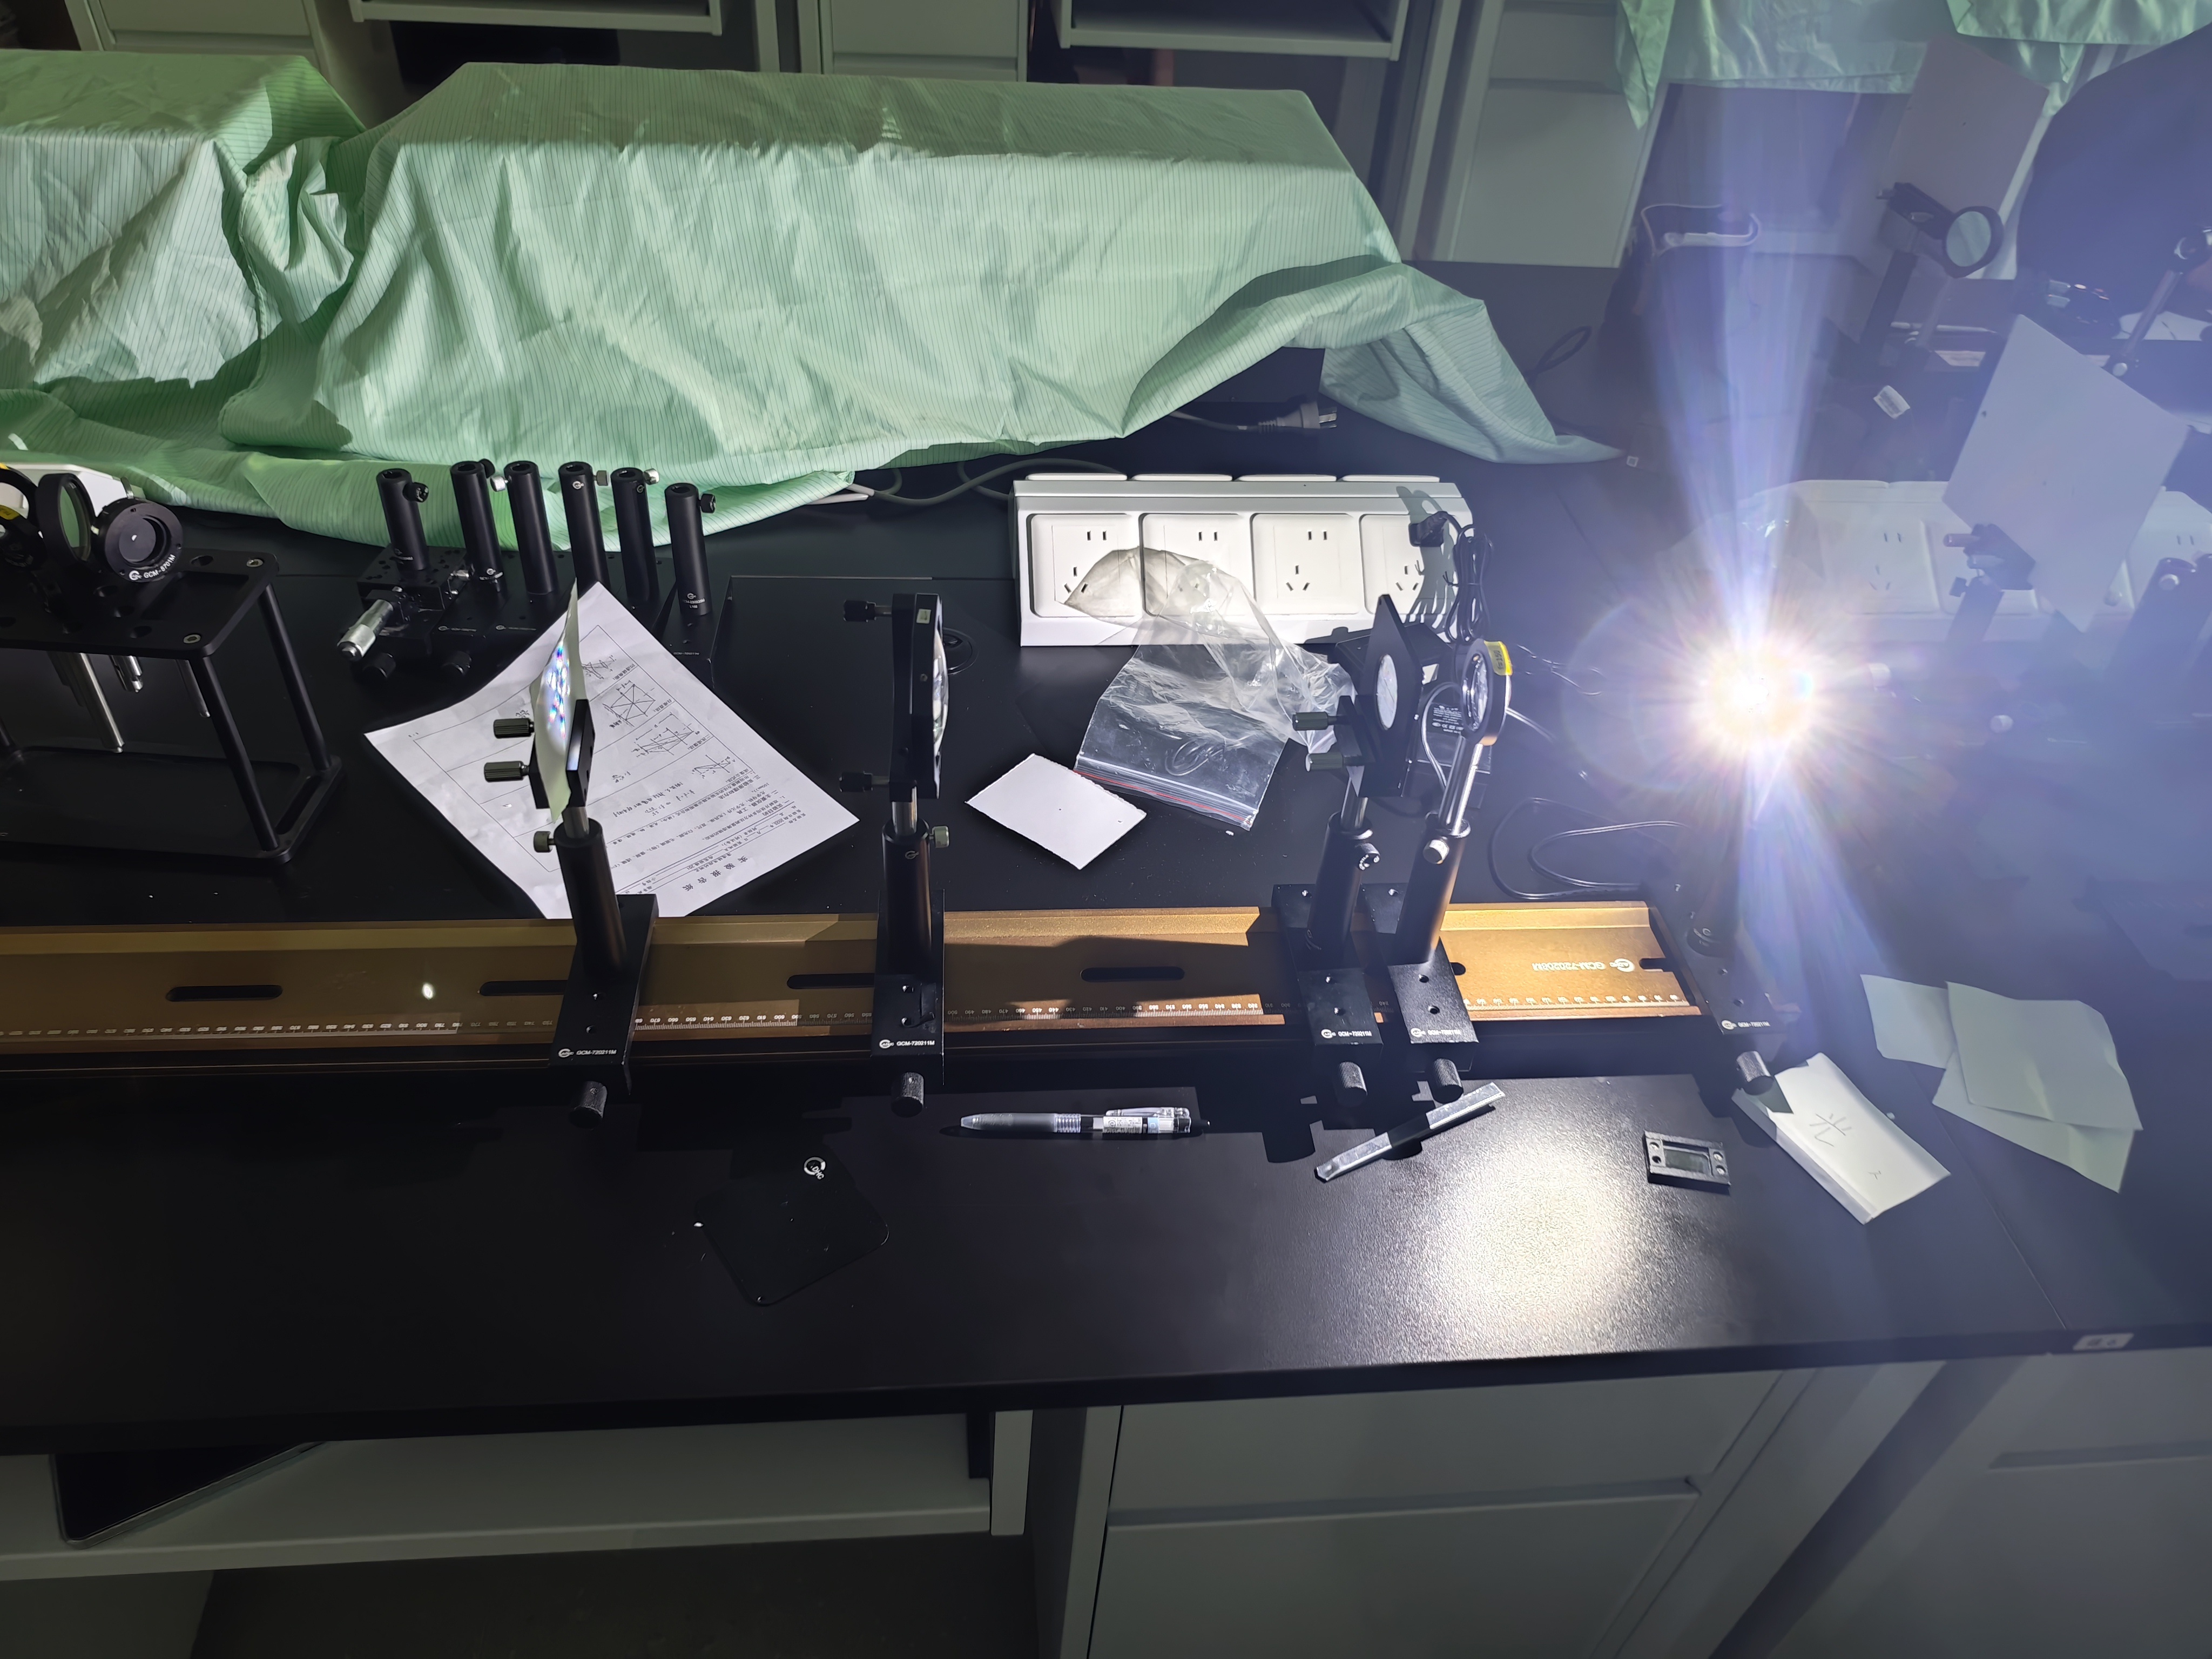
\includegraphics[width=0.25\textwidth]{fig24b.jpg}
    }
    \hspace{0.05\textwidth}
    \subfigure[成像图]{
        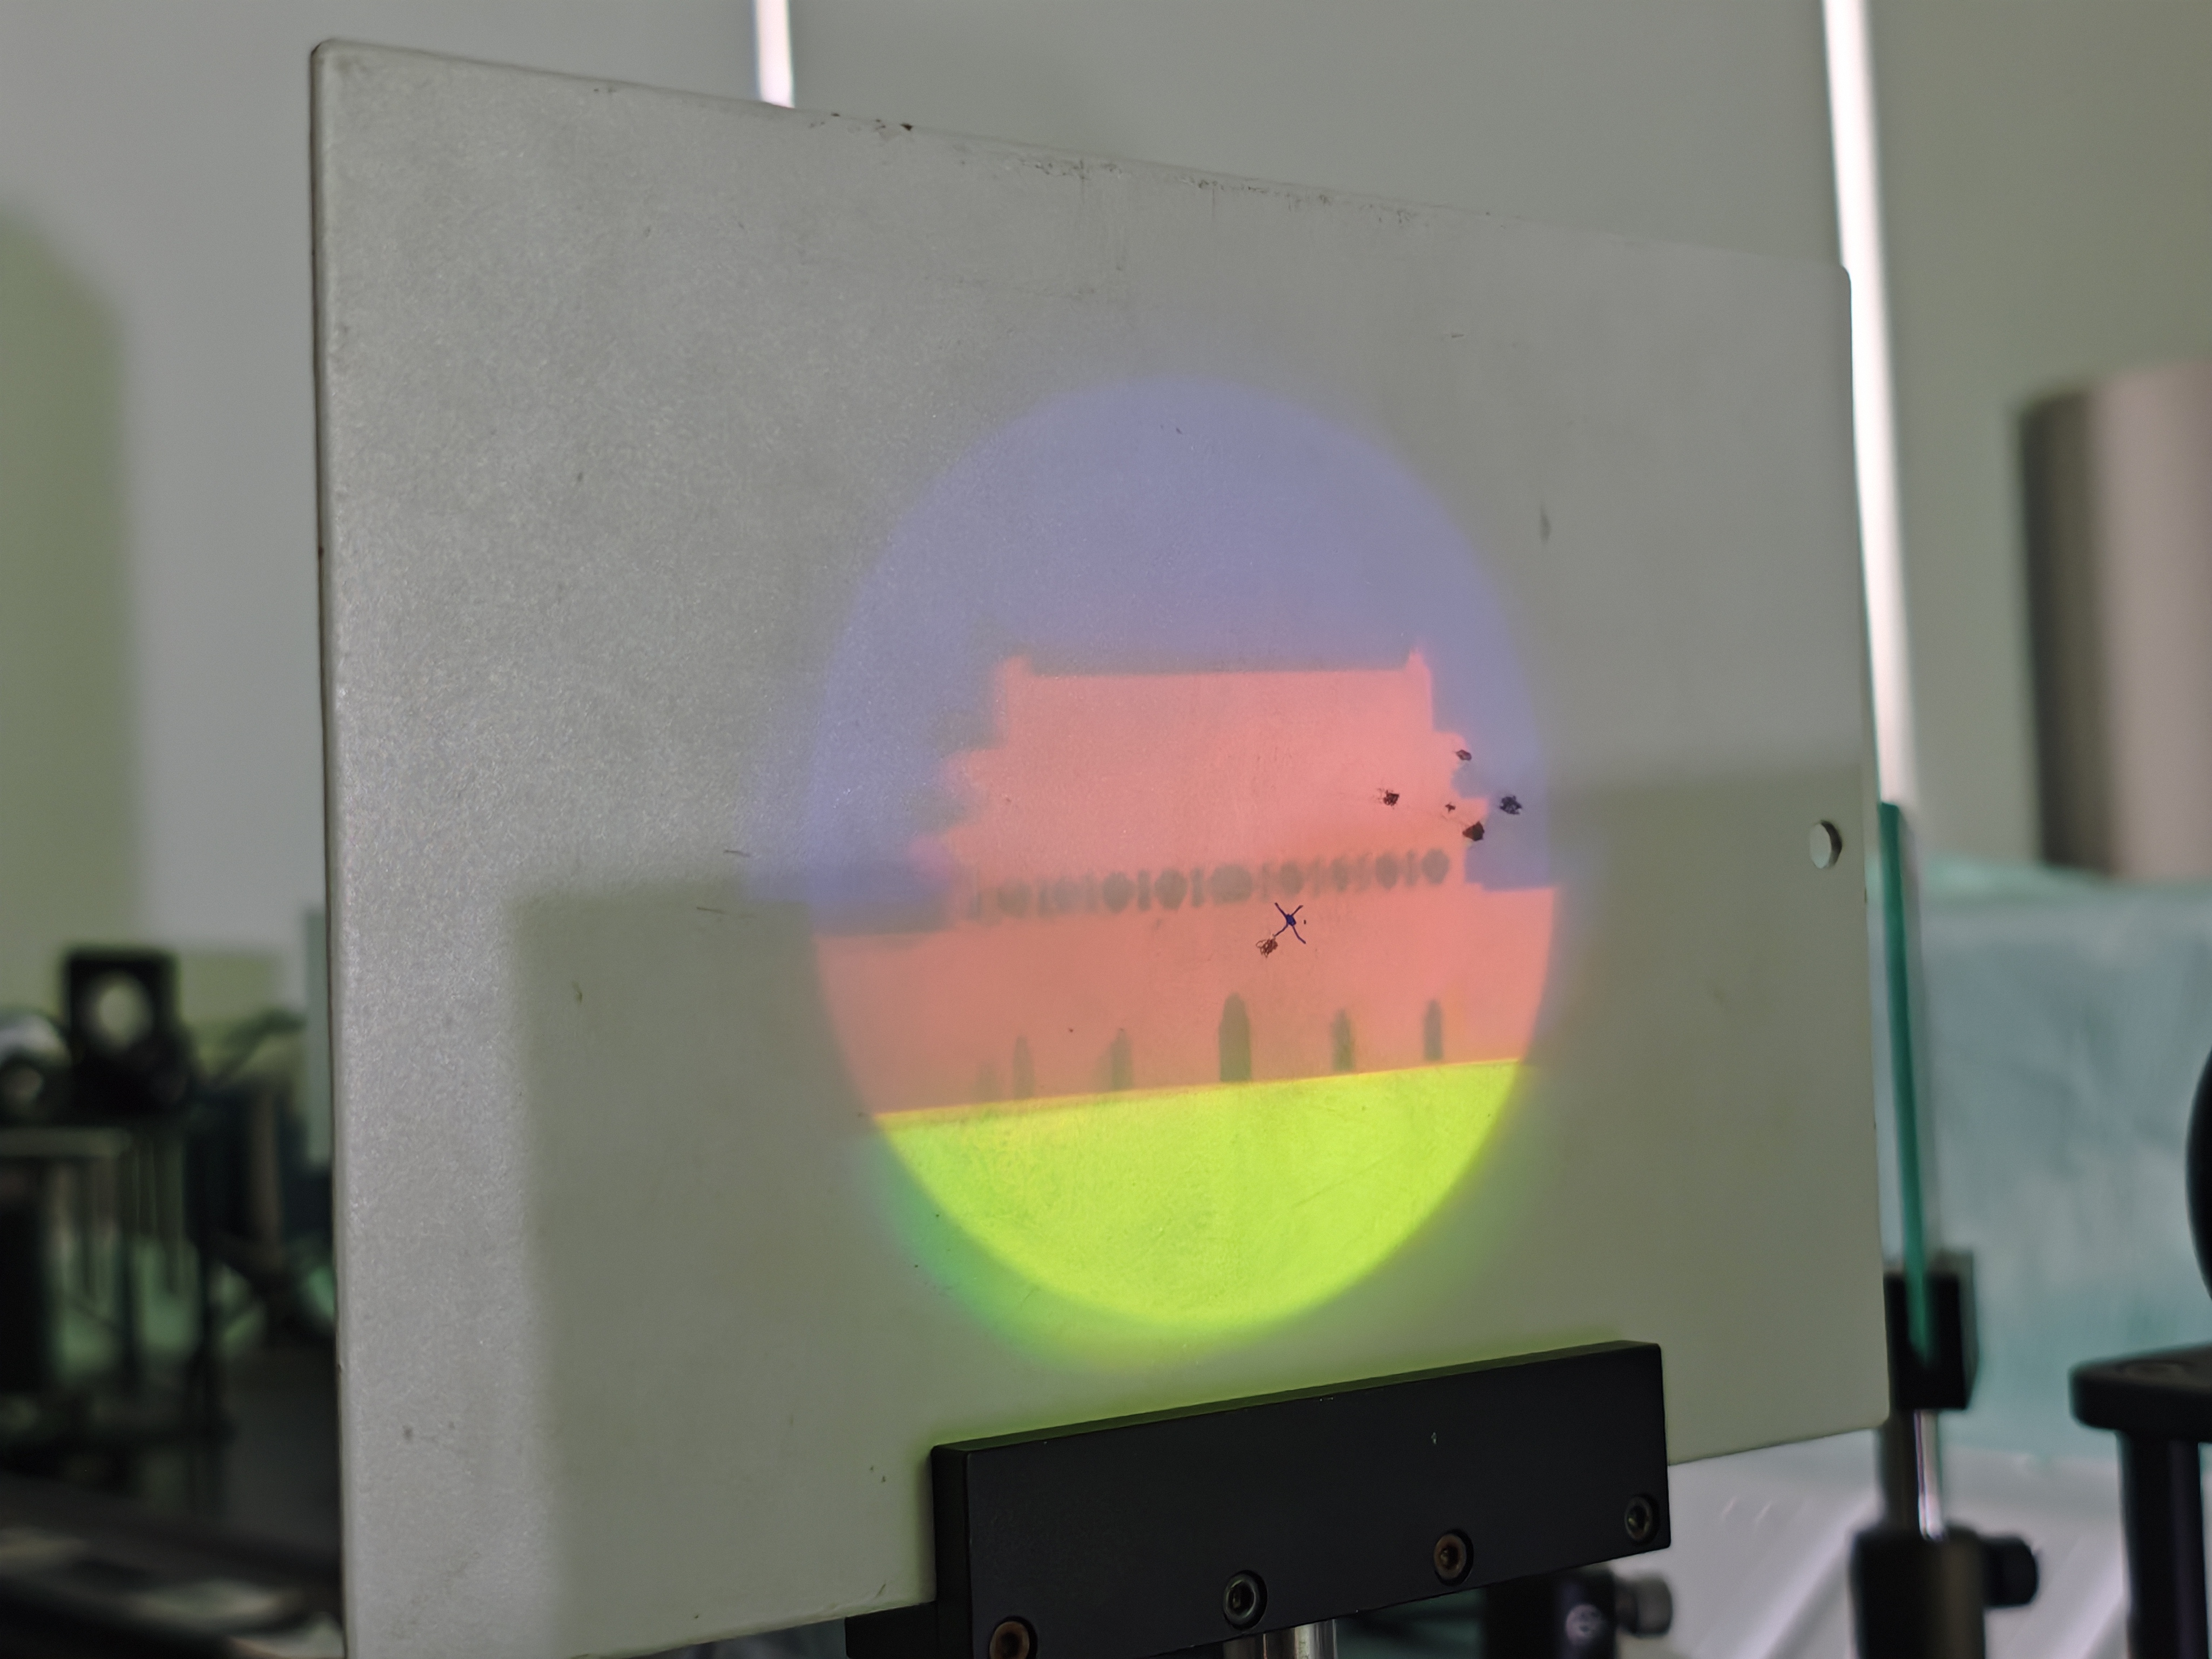
\includegraphics[width=0.25\textwidth]{fig24a.jpg}
    }
    \subfigure[频谱面图像]{
        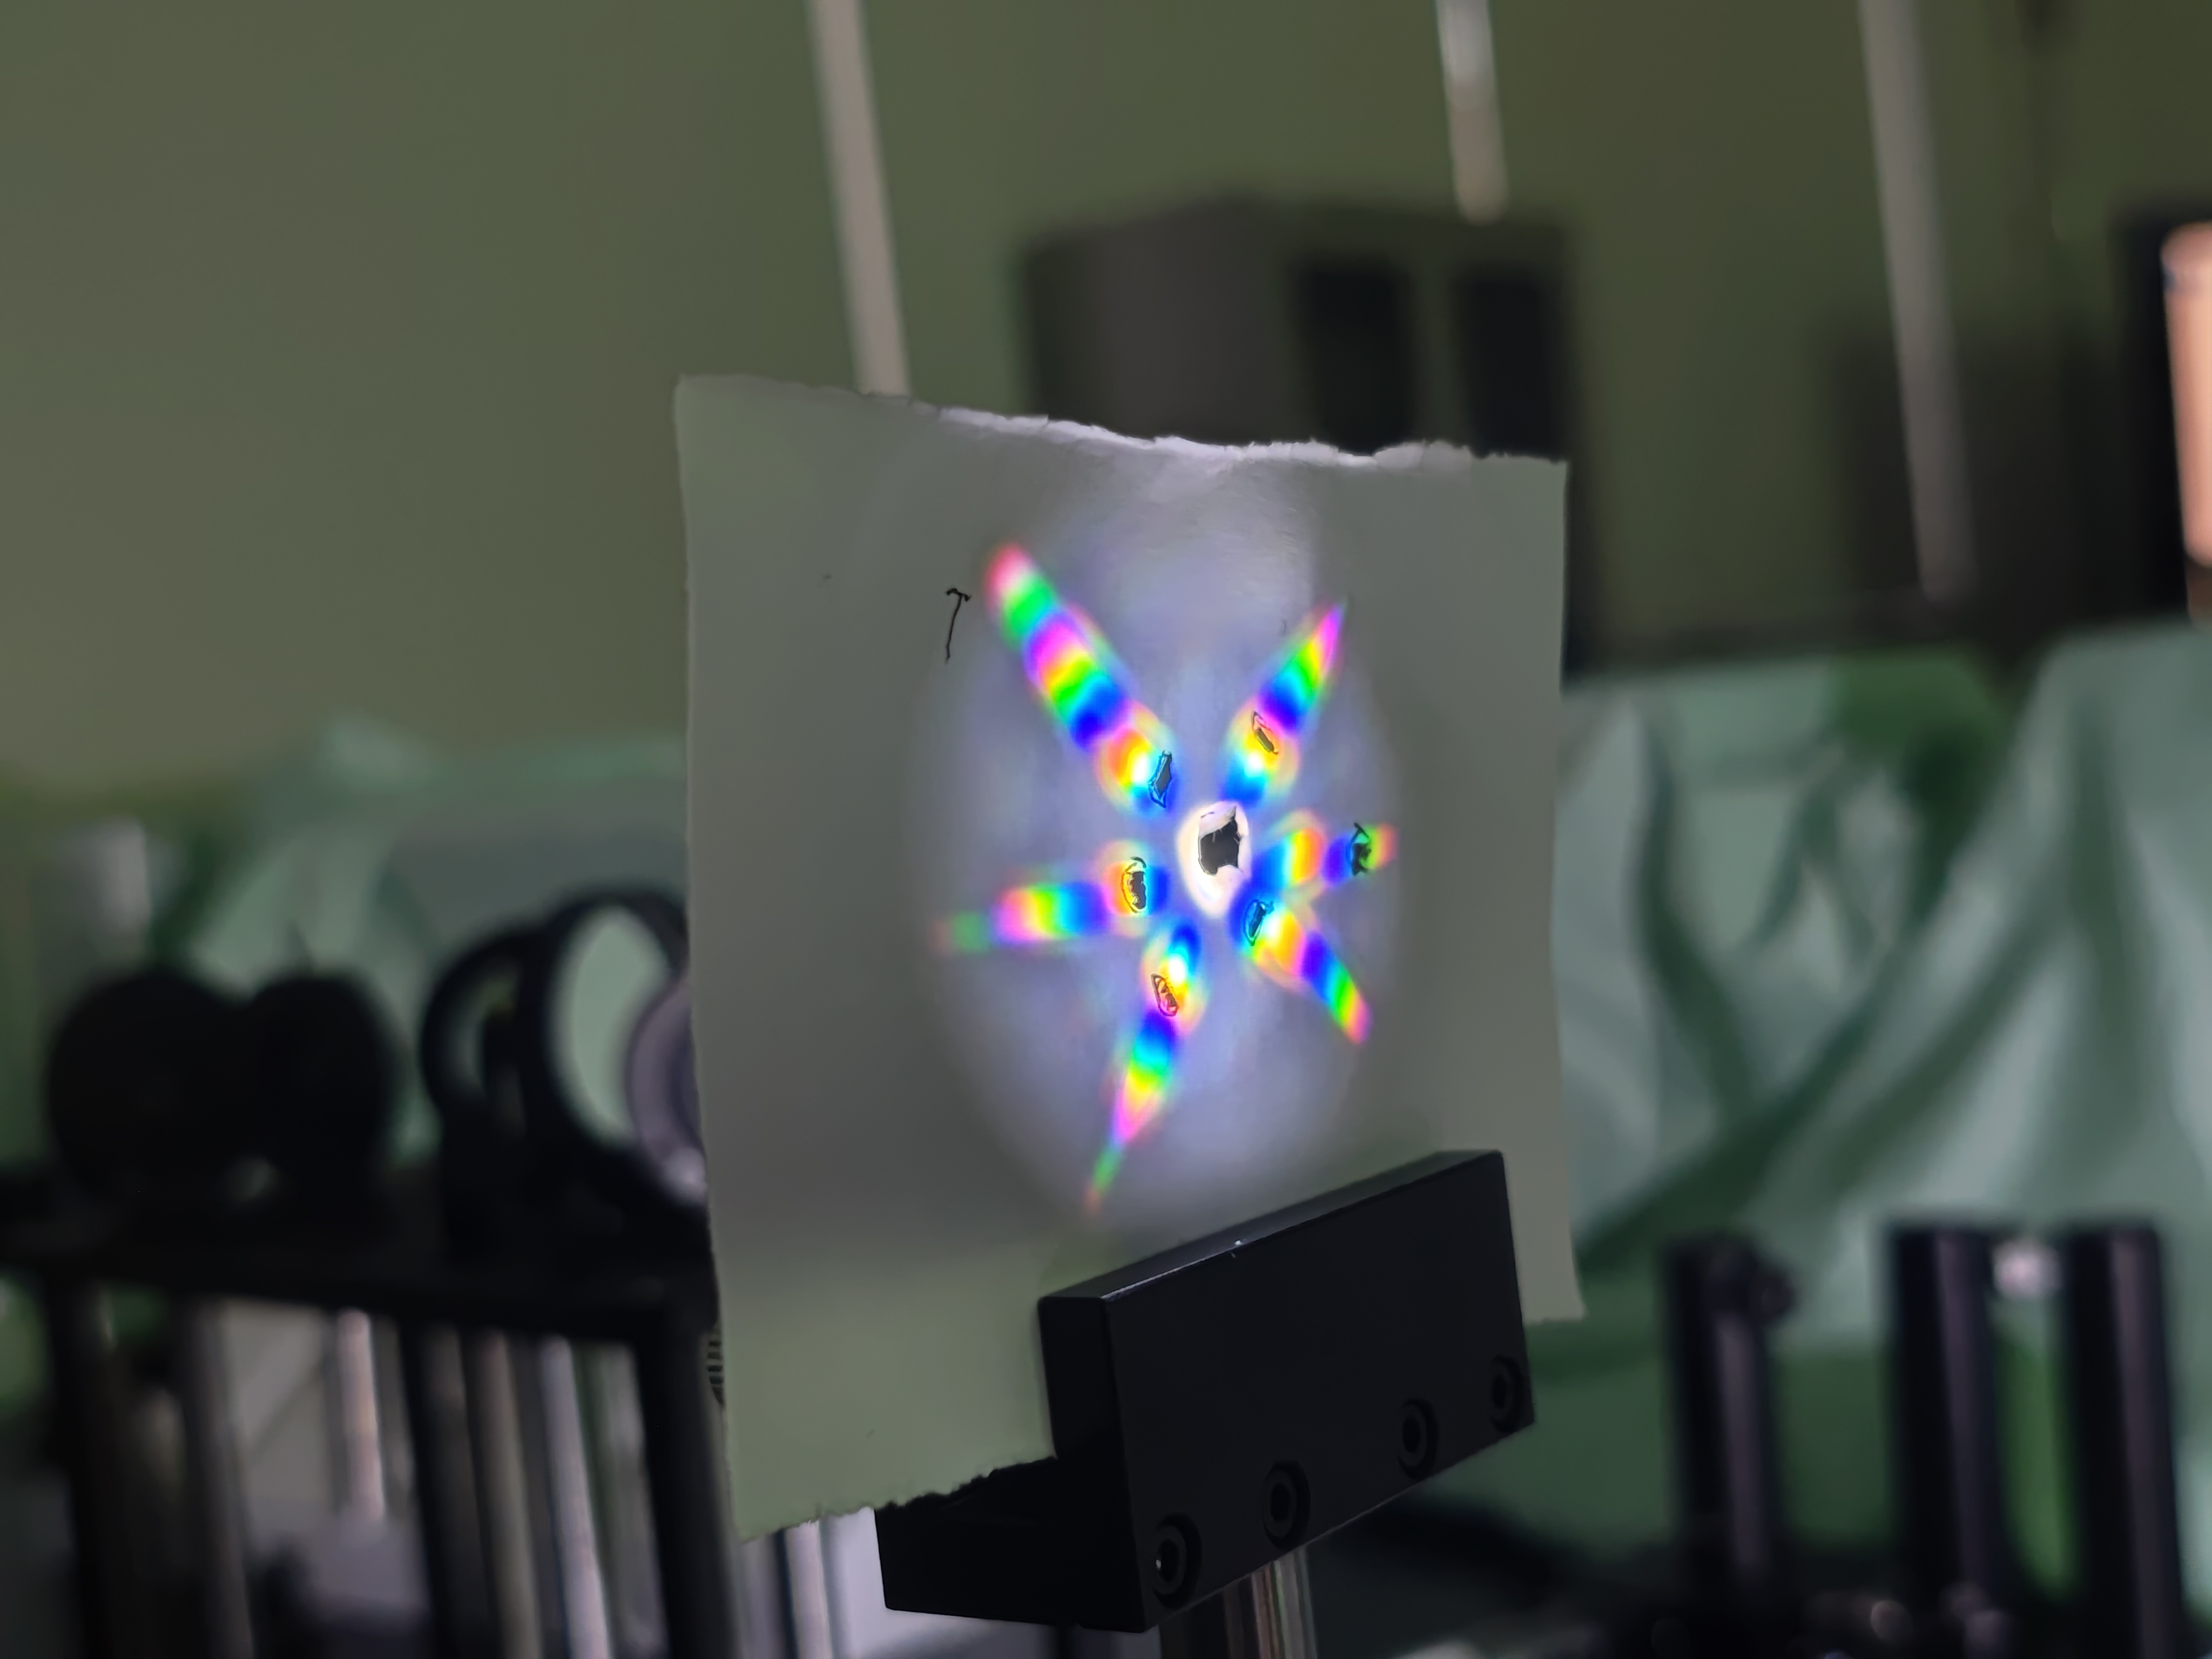
\includegraphics[width=0.25\textwidth]{fig24c.jpg}
    }
    \caption{θ调制假彩色编码结果3}
\end{figure}
\paragraph{通过在对应的频谱面放置自制滤波器}使用自制滤波器，同样实现了假彩色显示，验证了滤波器设计的有效性。
\paragraph{结果分析}
实验结果表明，θ调制与频谱面空间选色相结合能有效实现区域性假彩色编码：不同取向的光栅将各区域的主要空间频谱导向不同方位，白光的波长色散使得同一方向上的不同波长在频谱面上发生空间分离，从而通过定向滤波器选择性透过特定波段实现颜色分配。实验中天空、城楼与草地呈现蓝、红、绿三色，说明衍射方向选择性与滤波器匹配良好。

同时也观察到若干局限：一是颜色纯度受入射光谱（如LED光源绿光分量）和滤光片带宽限制，出现色带混叠和饱和度不足；二是空间分辨率与颜色分离之间存在权衡——为保证色散分离常需较大衍射角或较窄带通，可能导致高频细节（如窗户、门洞）被部分截断，从而在有些区域出现黑色或轮廓化现象；三是系统对滤波器位置和角度敏感，微小错位会引起色彩偏移或局部失真。

建议改进方向包括：使用光谱较均匀的光源或校正光谱分量、采用带通更窄且中心波长可调的滤片以提高颜色纯度、并通过精细对位与微调滤波器开孔位置以减少高频信息的误阻断。此外，可对频谱面图像进行拍照并量化分析谱带位置与滤光器响应，以便定量评估颜色分配的空间与波长映射关系。

\subsection{夫琅和费衍射与菲涅尔衍射实验结果}

\begin{figure}[htbp]
    \centering
    \subfigure[]{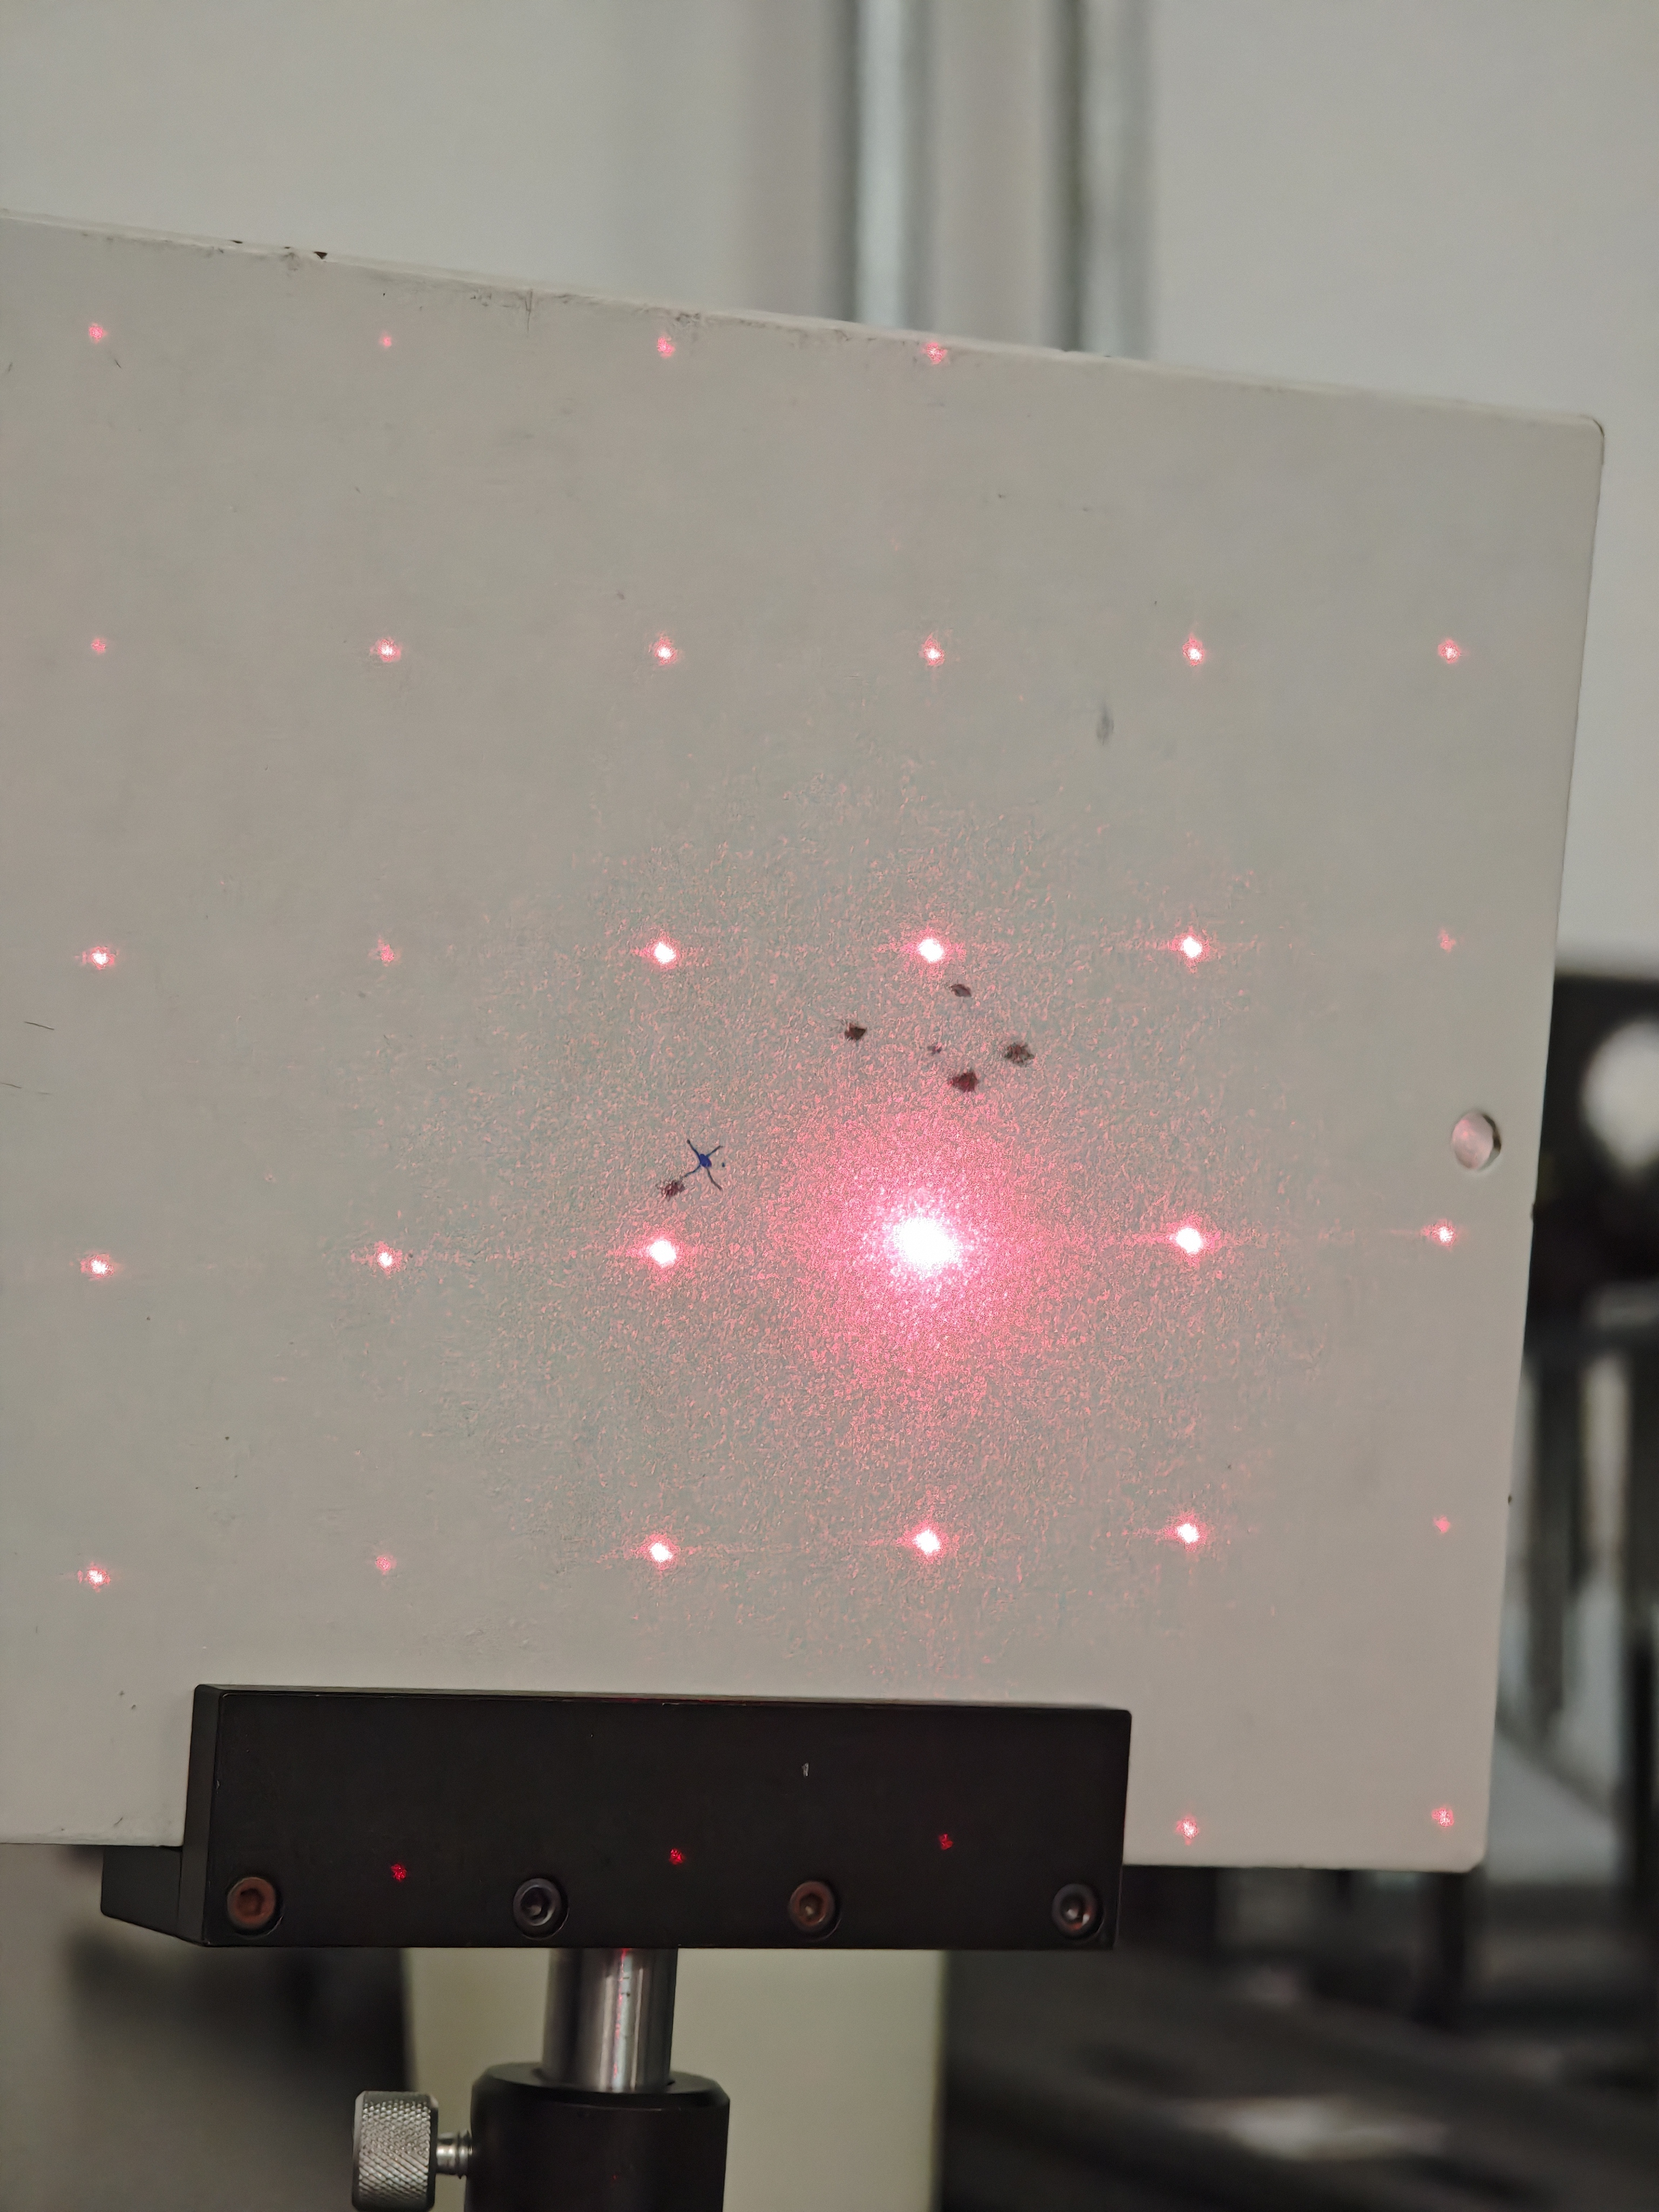
\includegraphics[width=0.24\textwidth]{fig/IMG_20251105_165247.jpg}}
    \subfigure[]{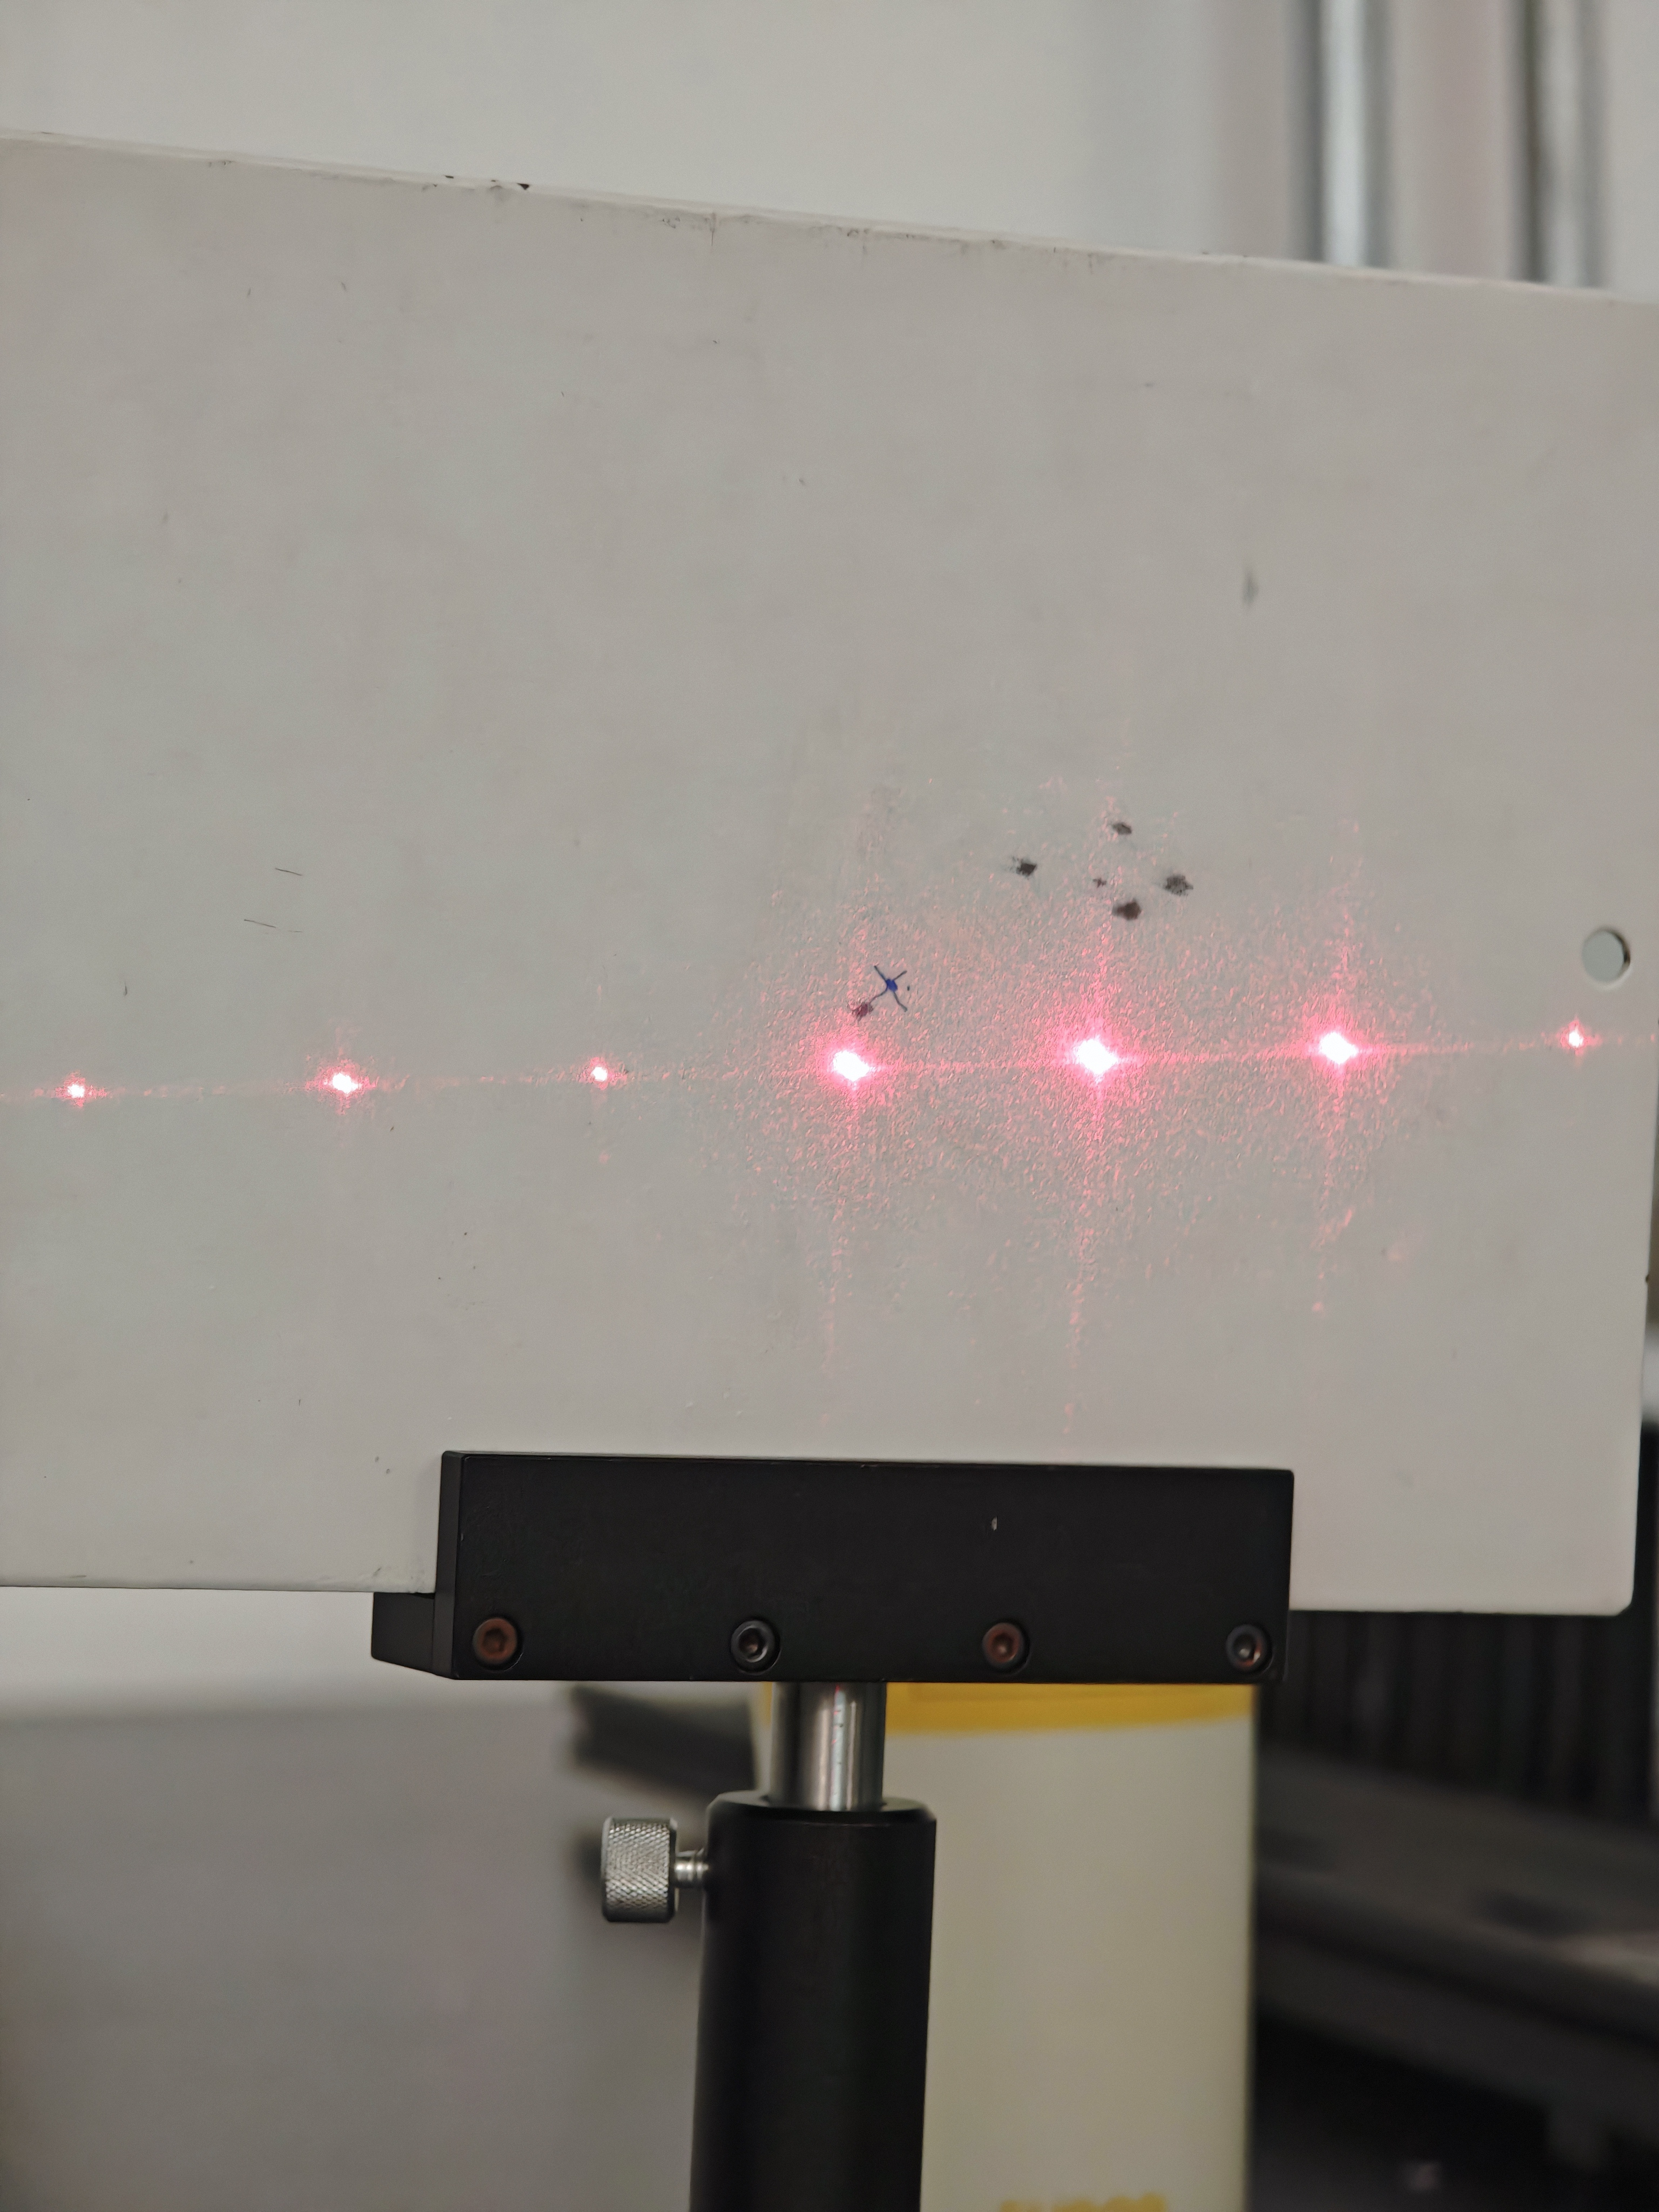
\includegraphics[width=0.24\textwidth]{fig/IMG_20251105_165255.jpg}}
    \subfigure[]{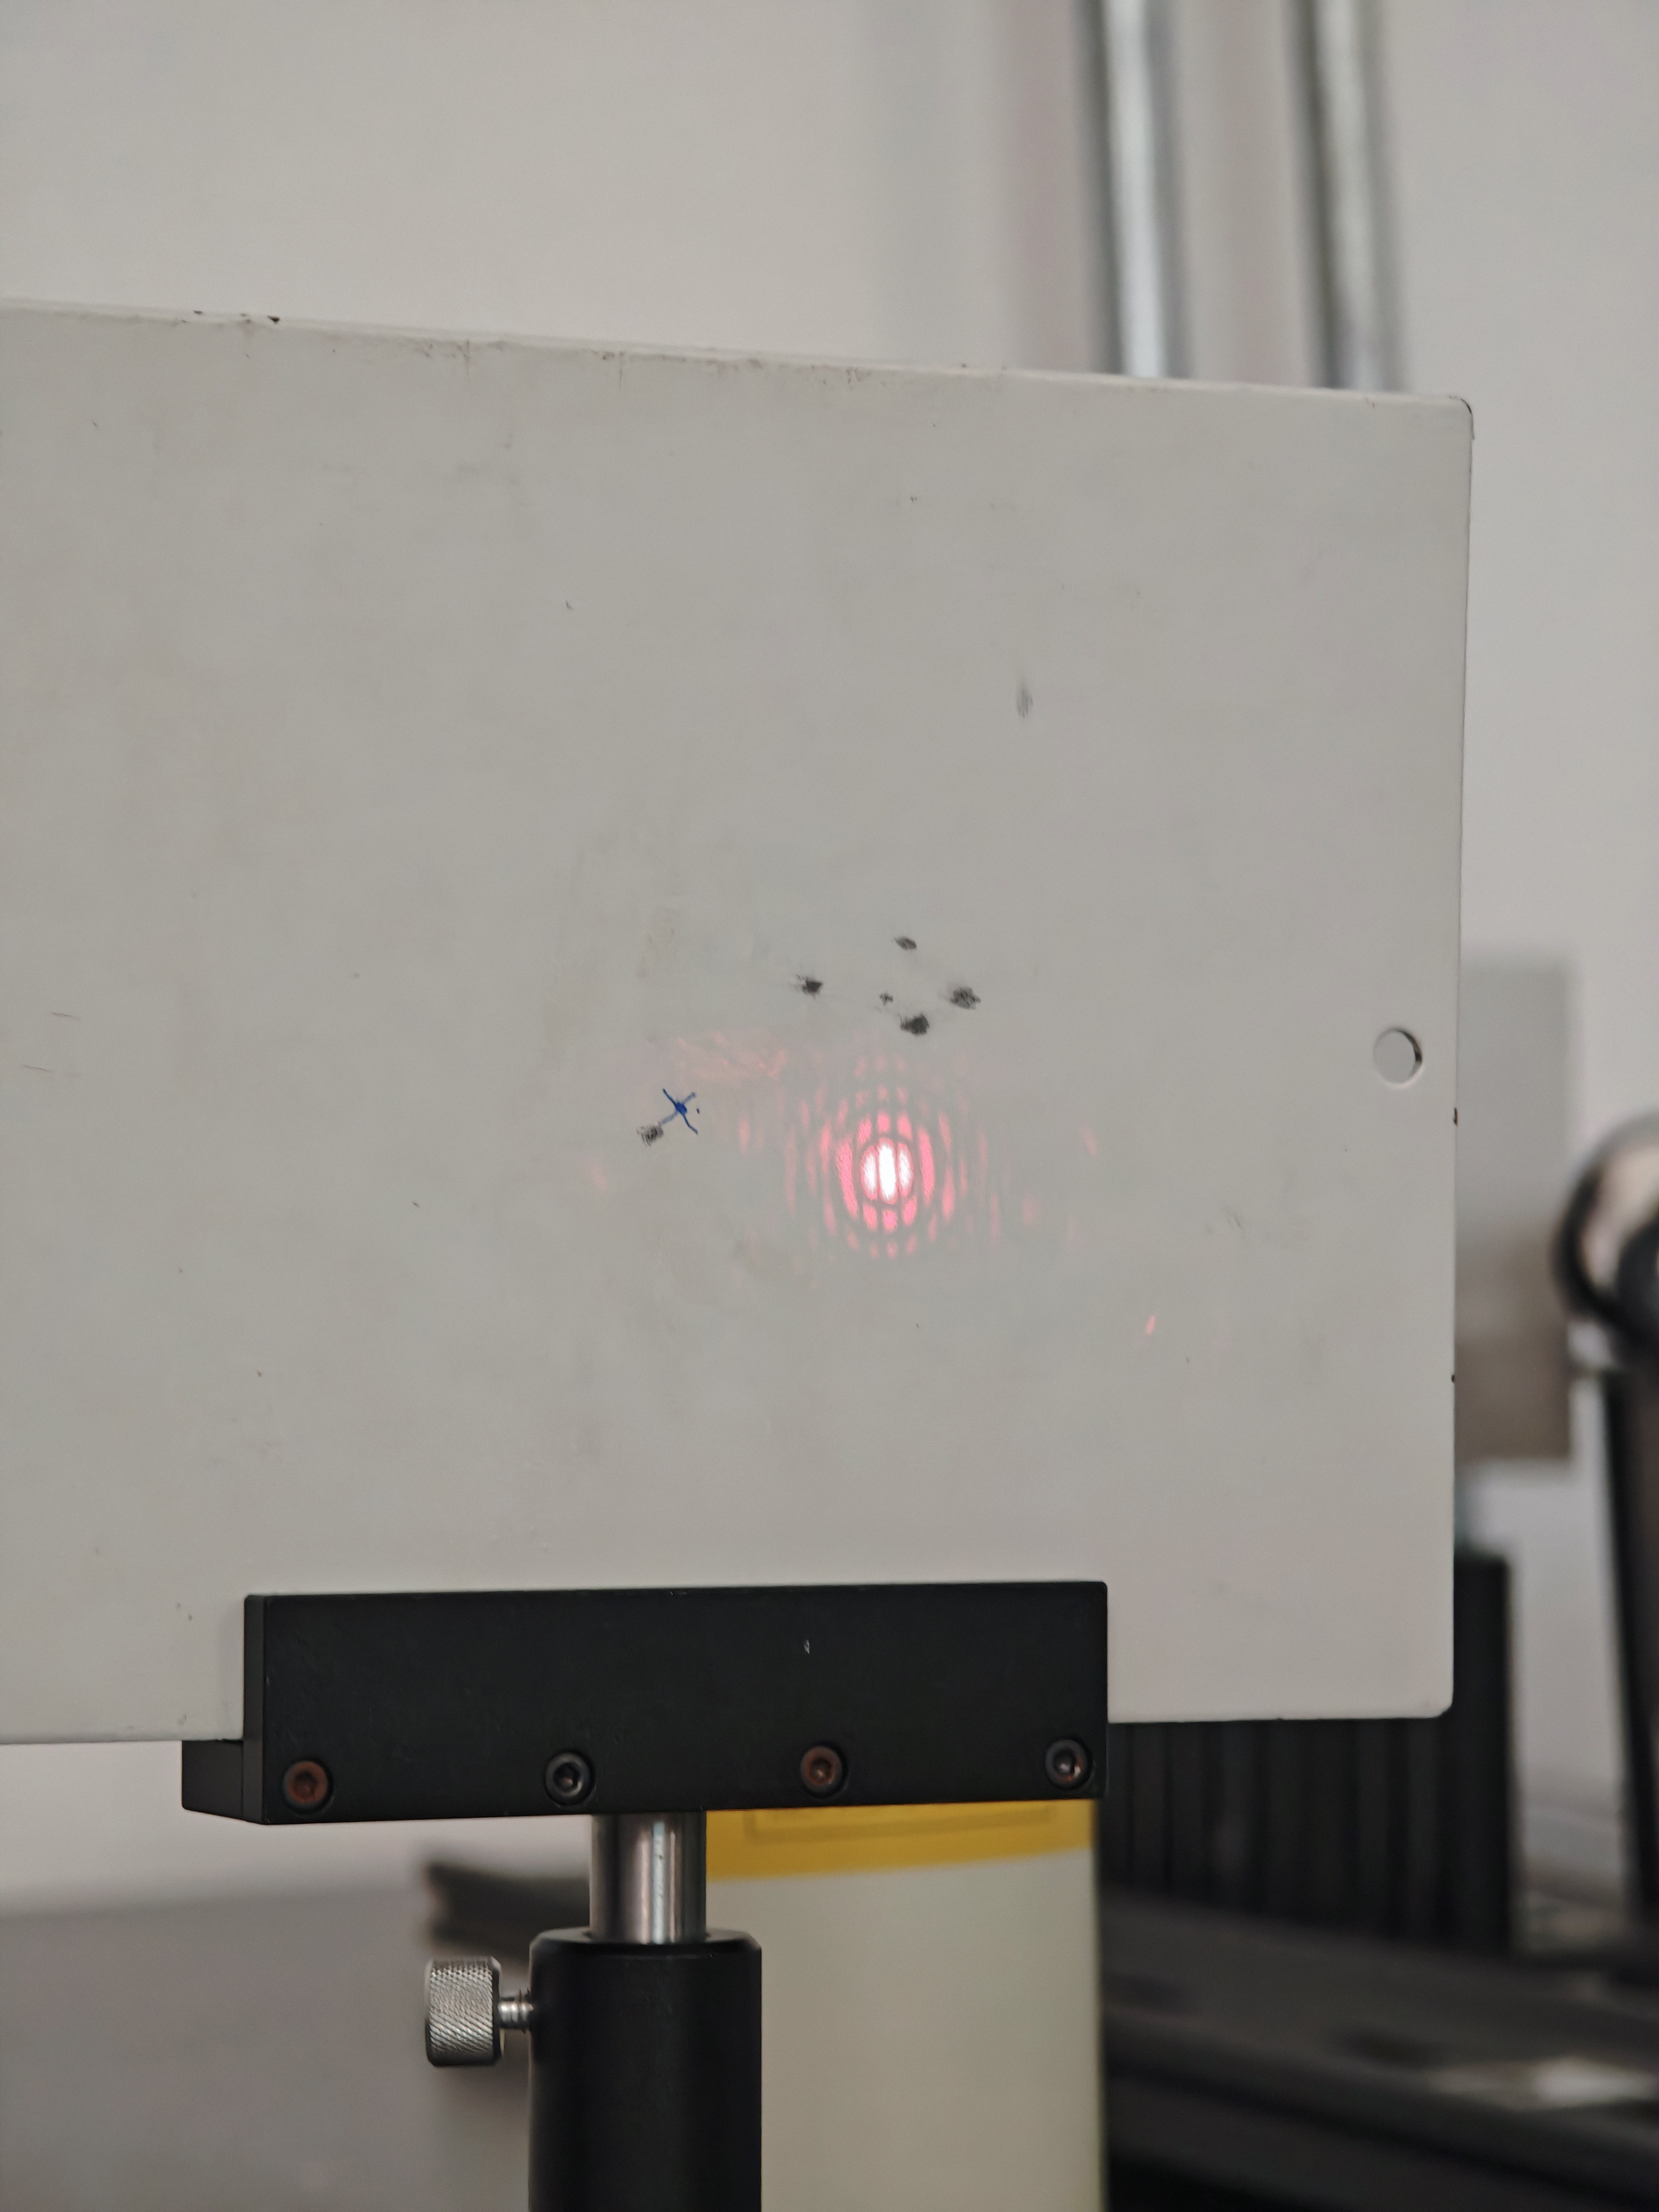
\includegraphics[width=0.24\textwidth]{fig/IMG_20251105_165300.jpg}}
    \subfigure[]{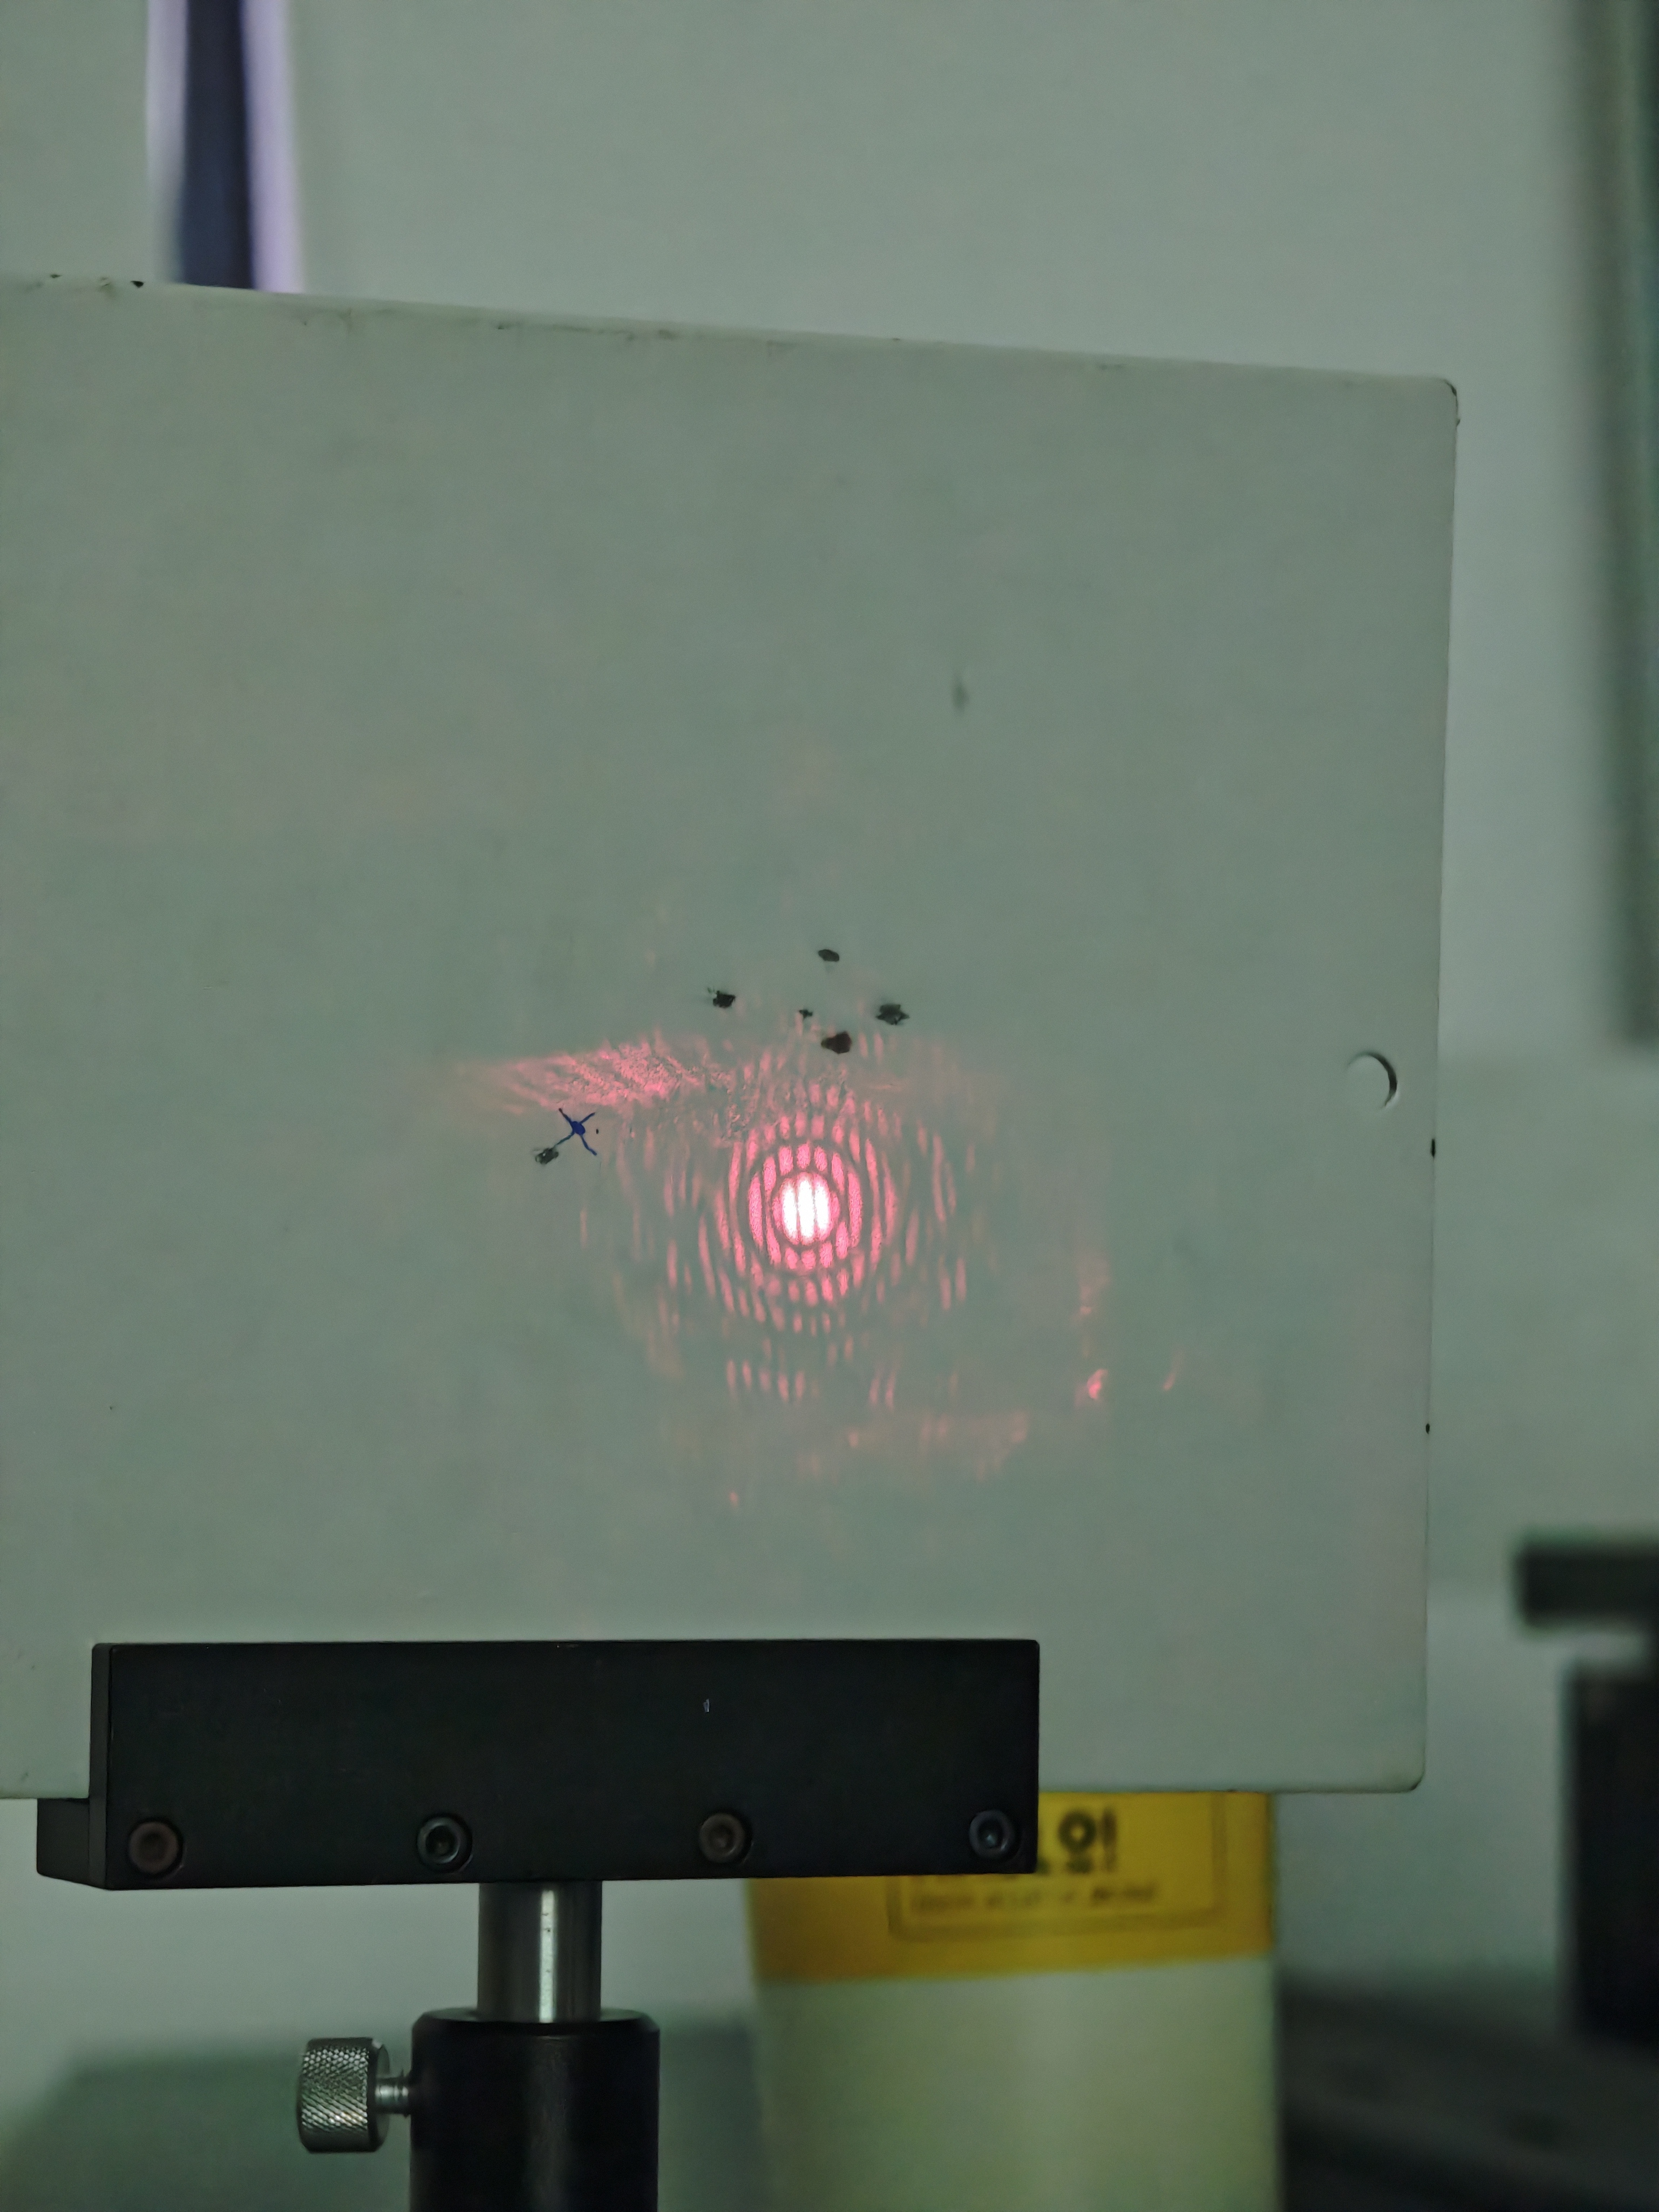
\includegraphics[width=0.24\textwidth]{fig/IMG_20251105_165405.jpg}}
    \subfigure[]{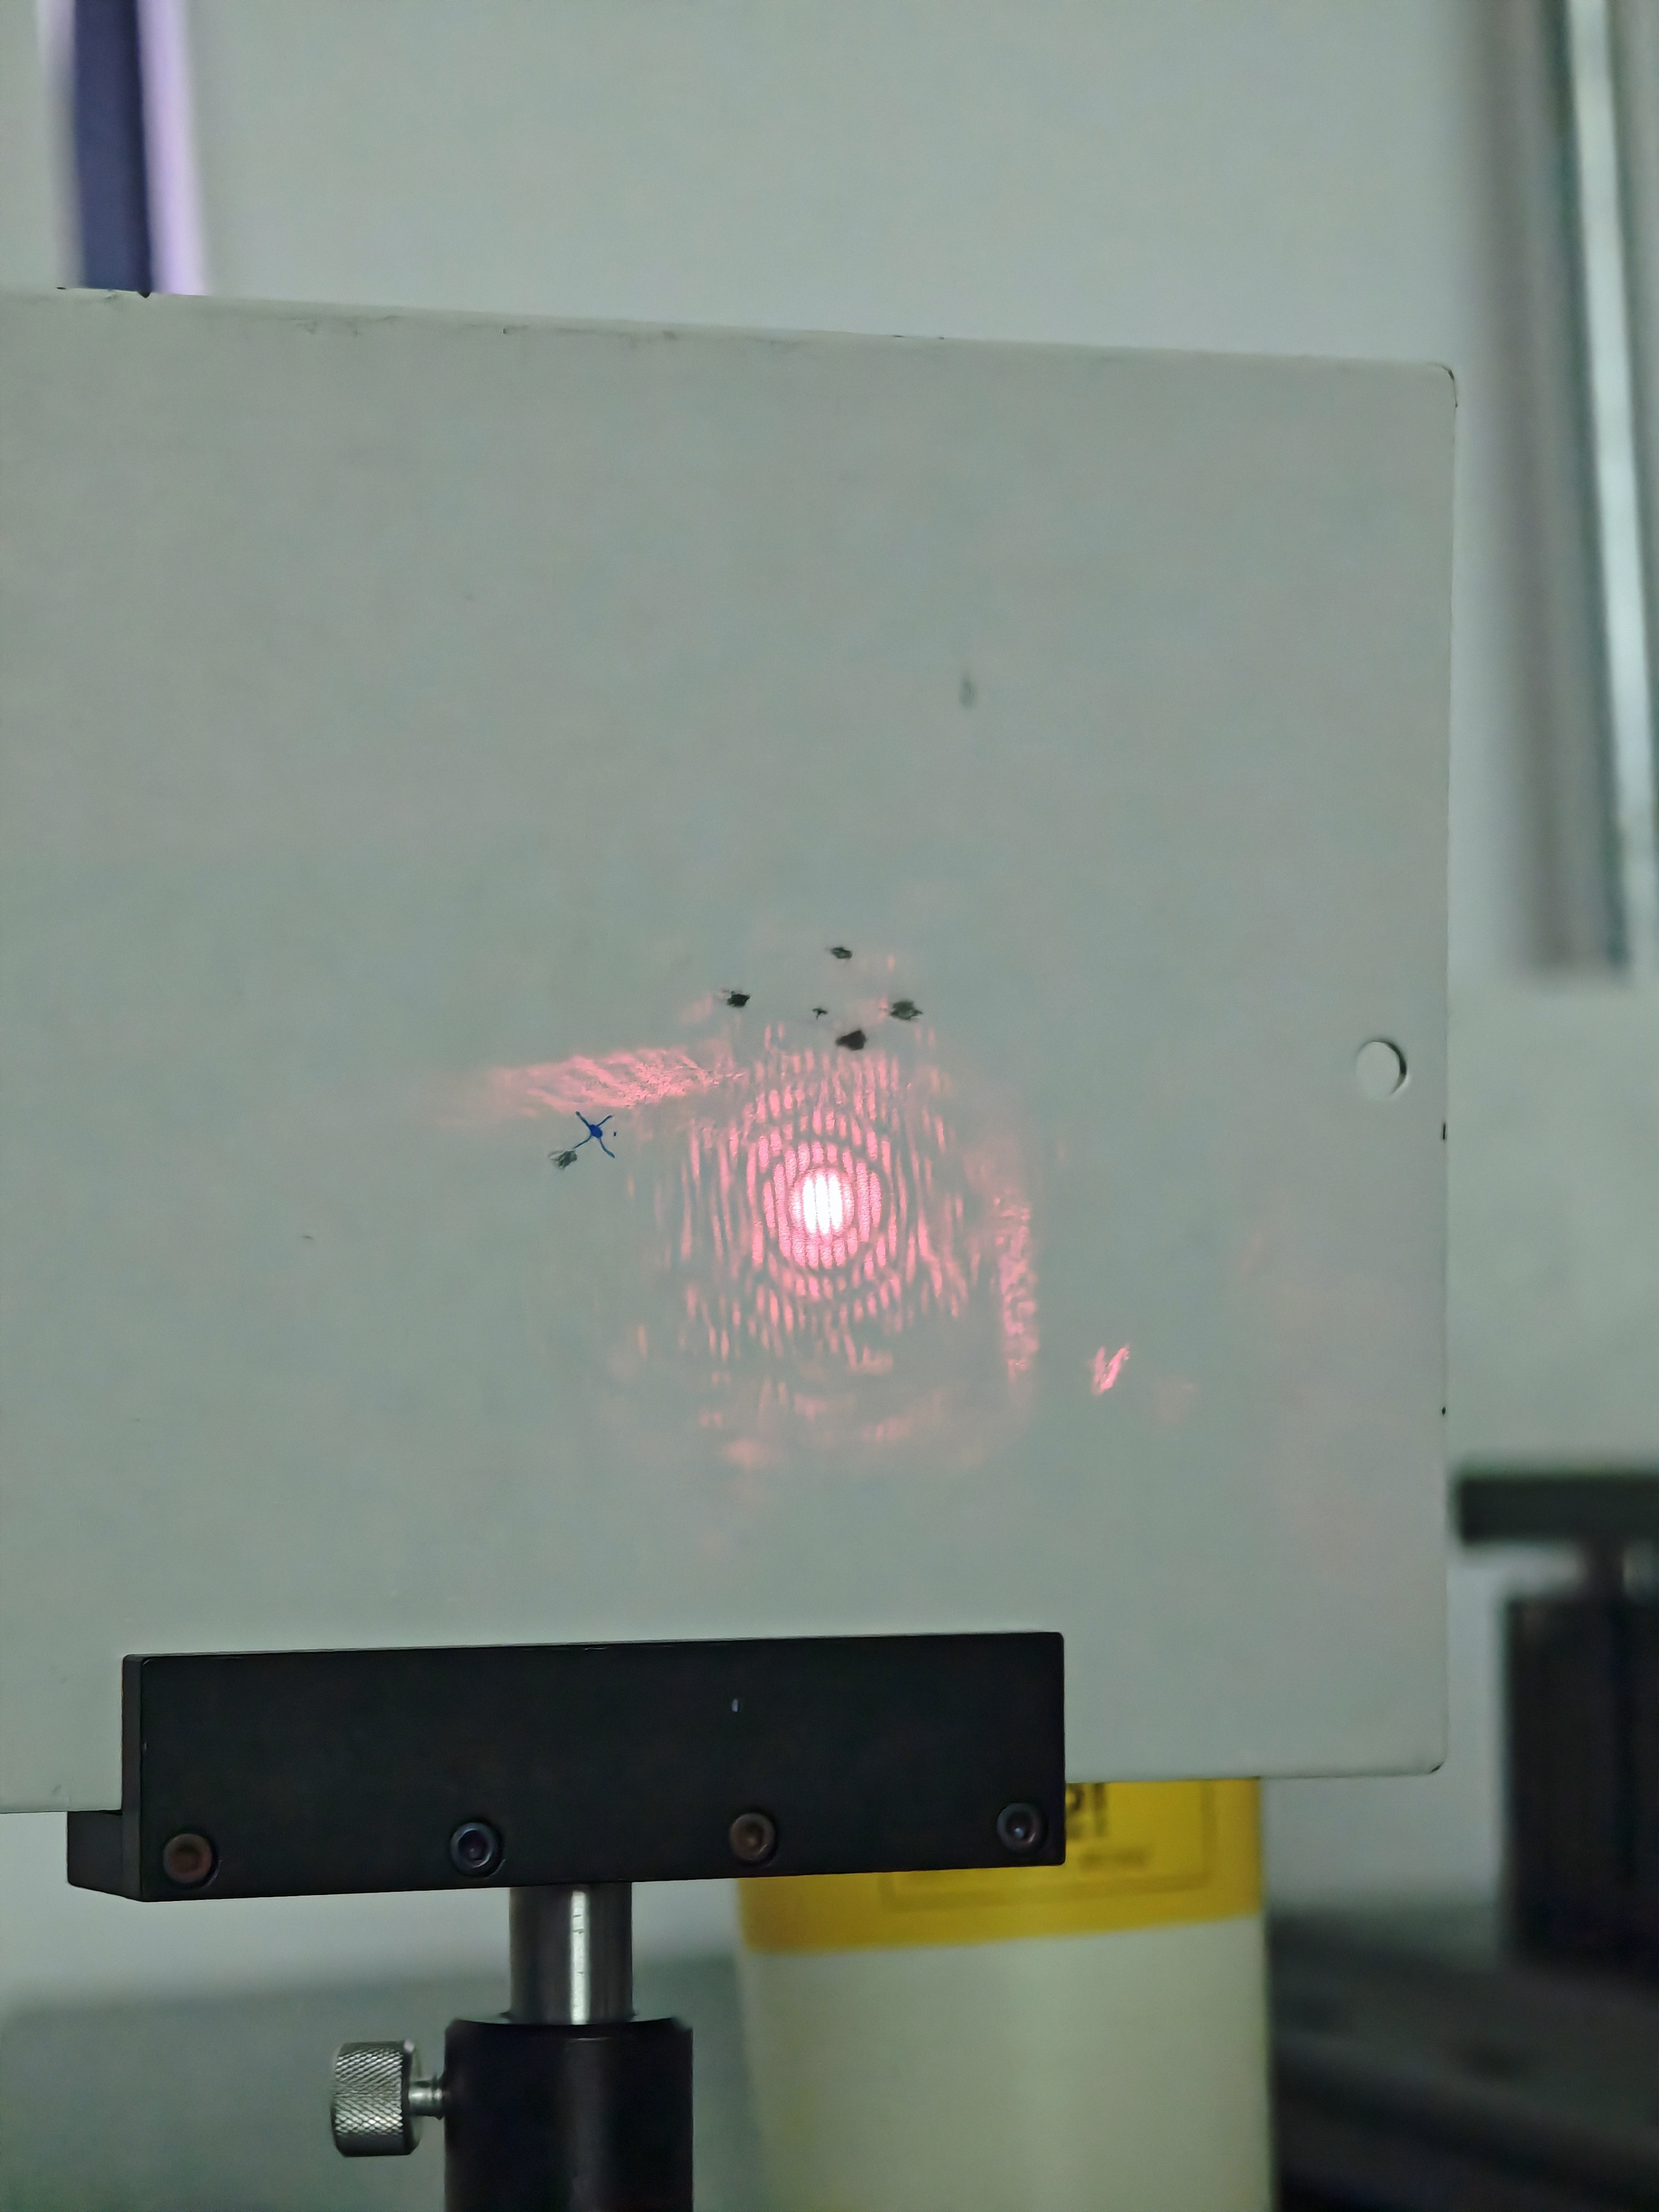
\includegraphics[width=0.24\textwidth]{fig/IMG_20251105_165411.jpg}}
    \subfigure[]{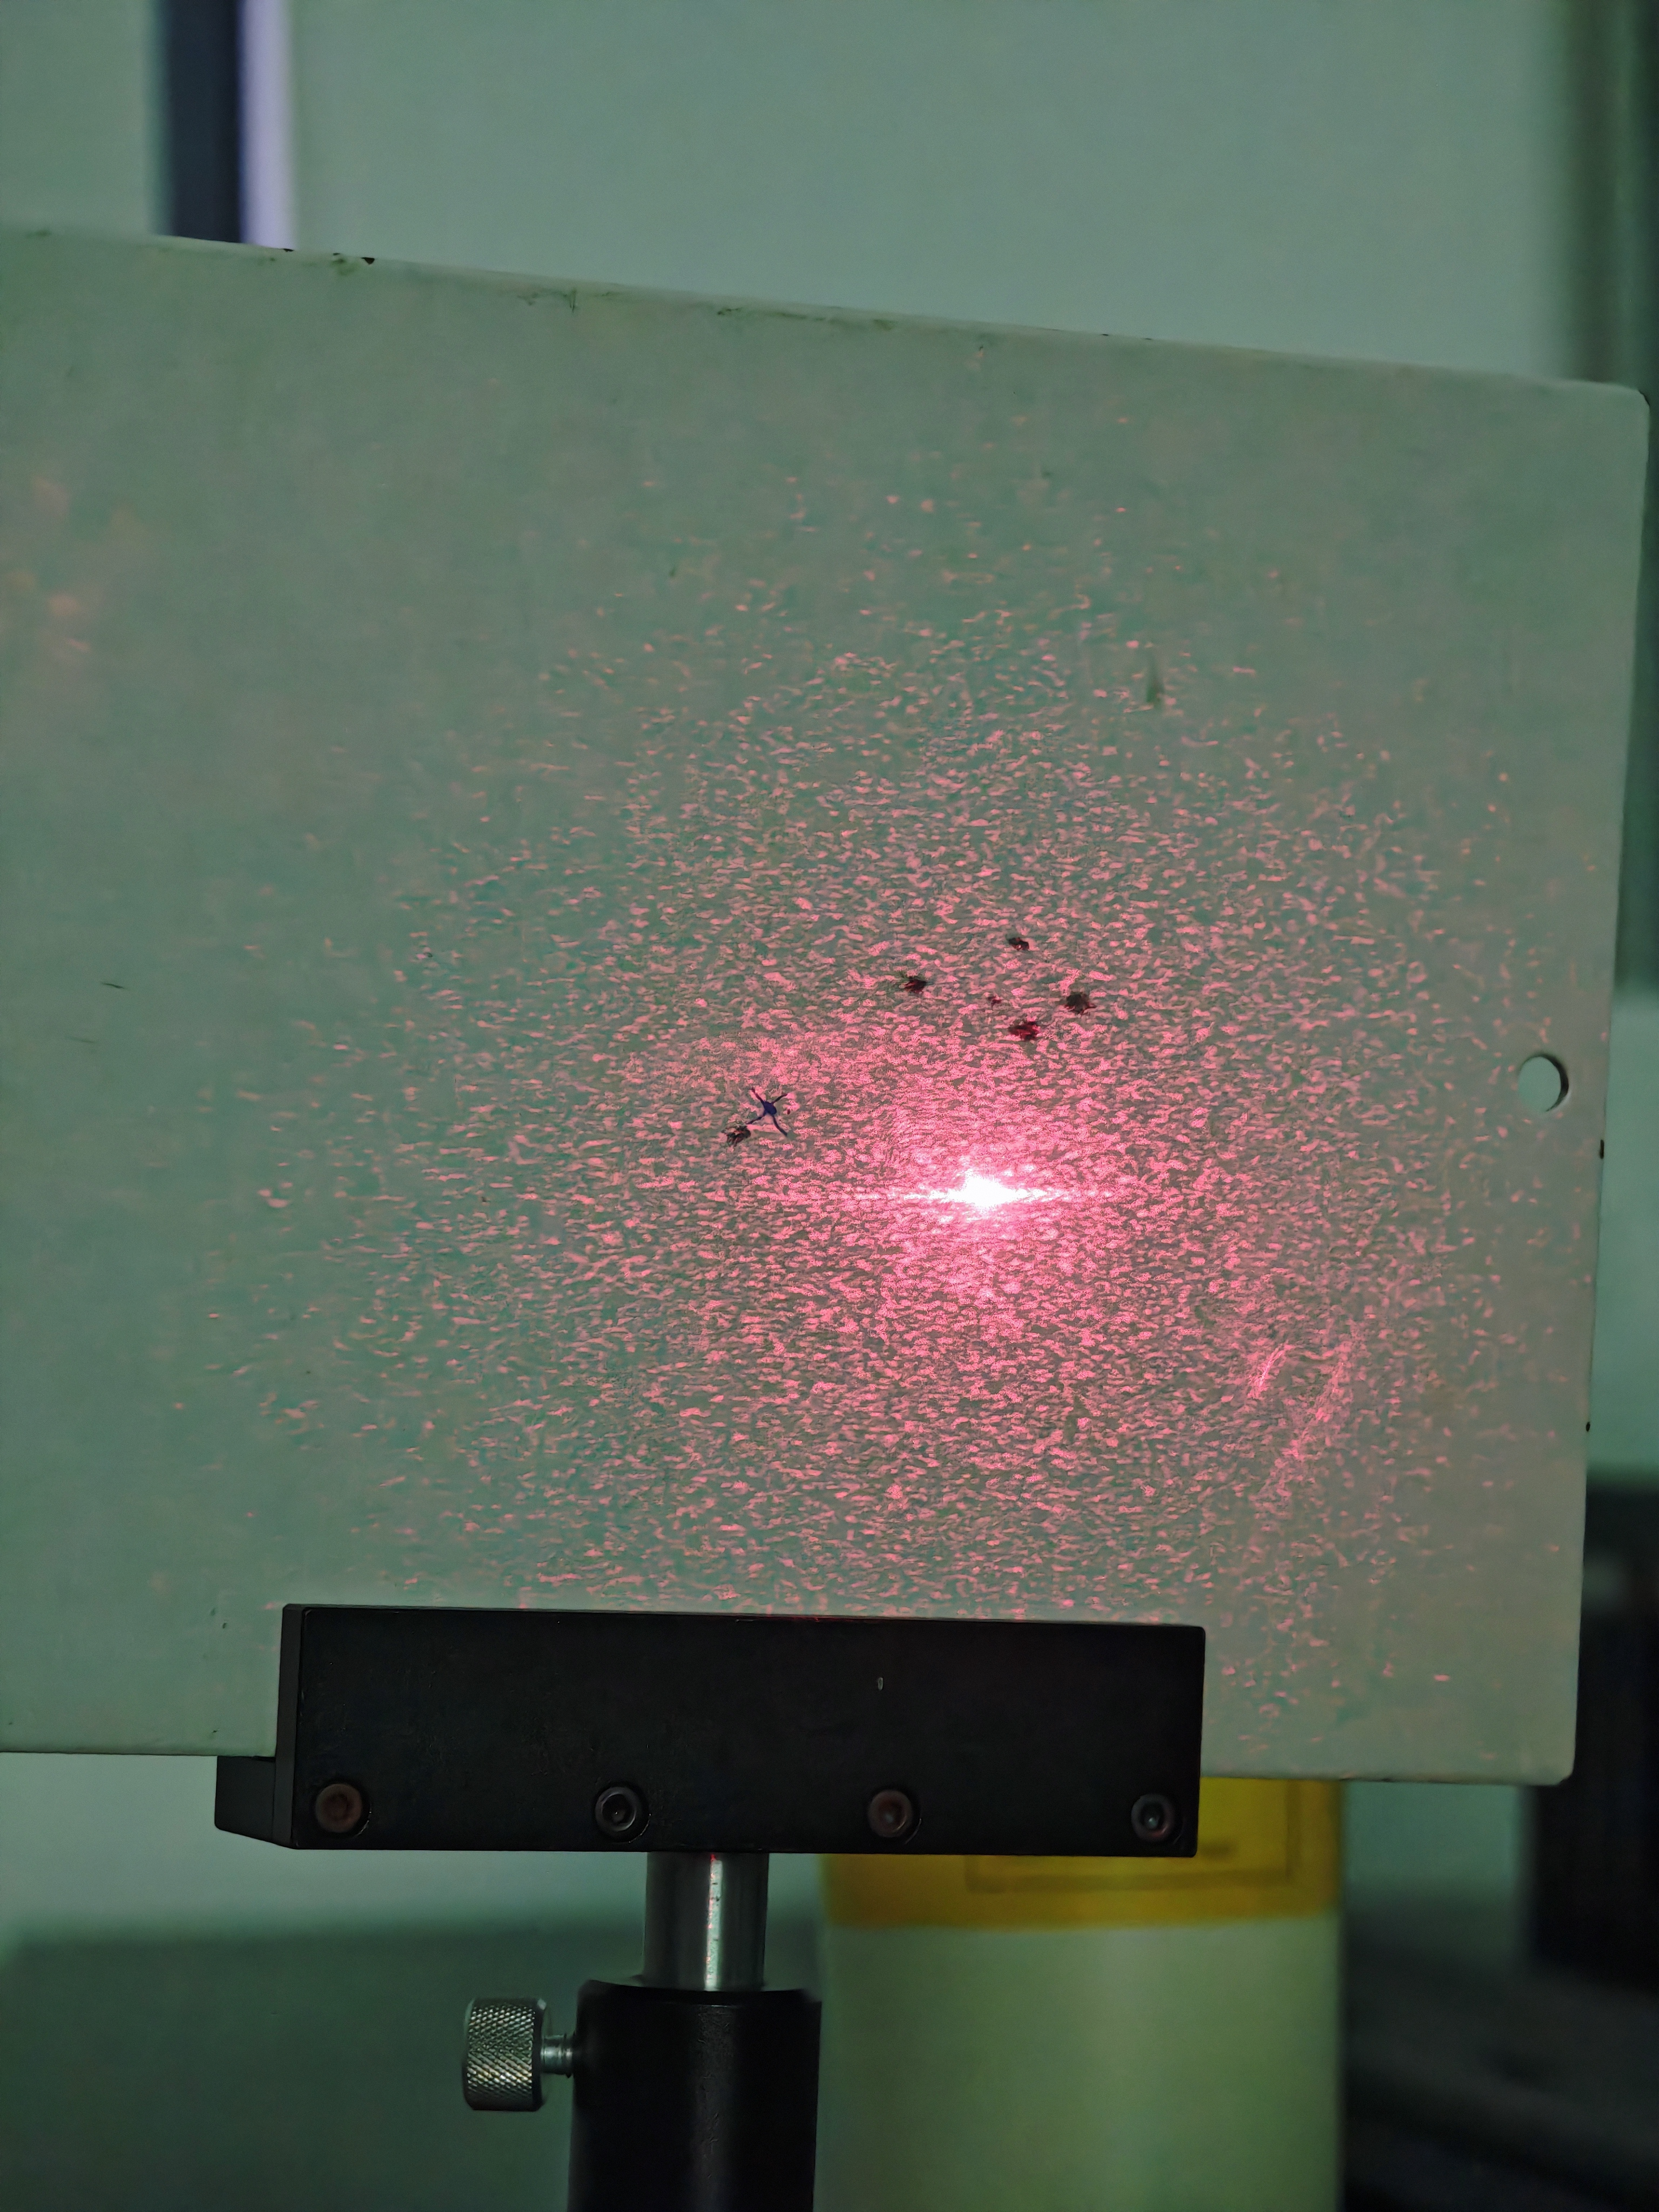
\includegraphics[width=0.24\textwidth]{fig/IMG_20251105_165424.jpg}}
    \subfigure[]{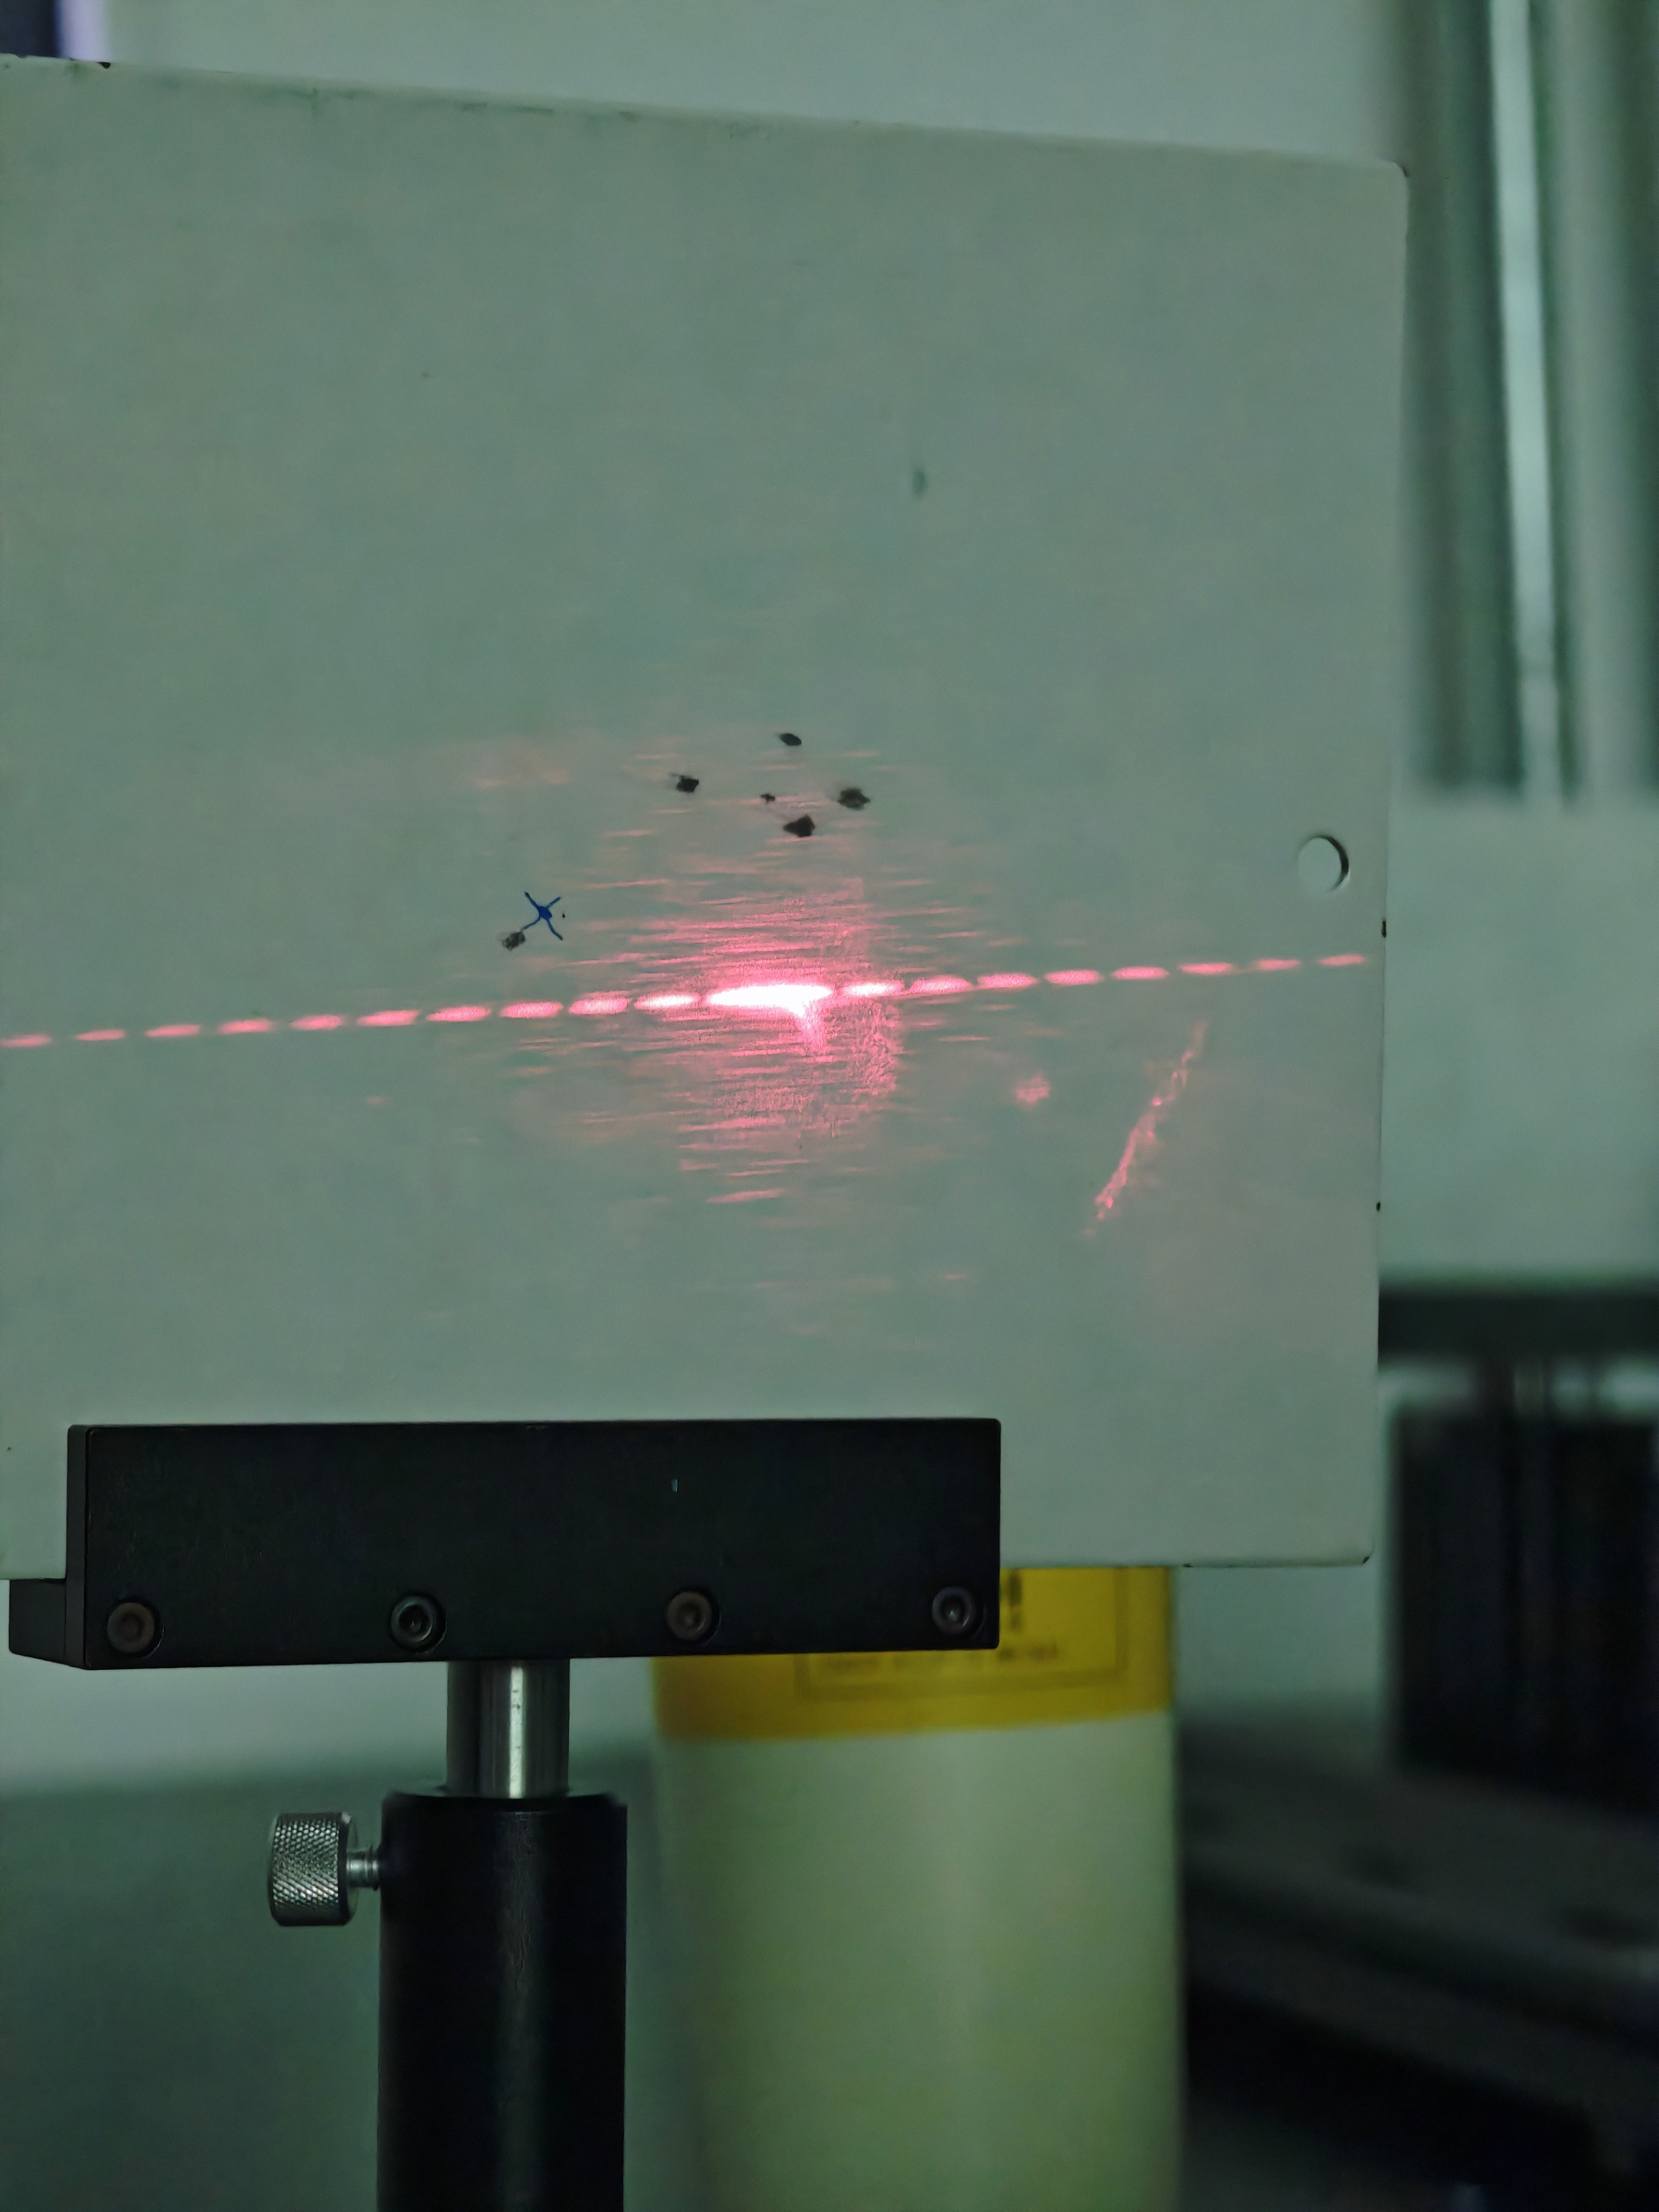
\includegraphics[width=0.24\textwidth]{fig/IMG_20251105_165433.jpg}}
    \subfigure[]{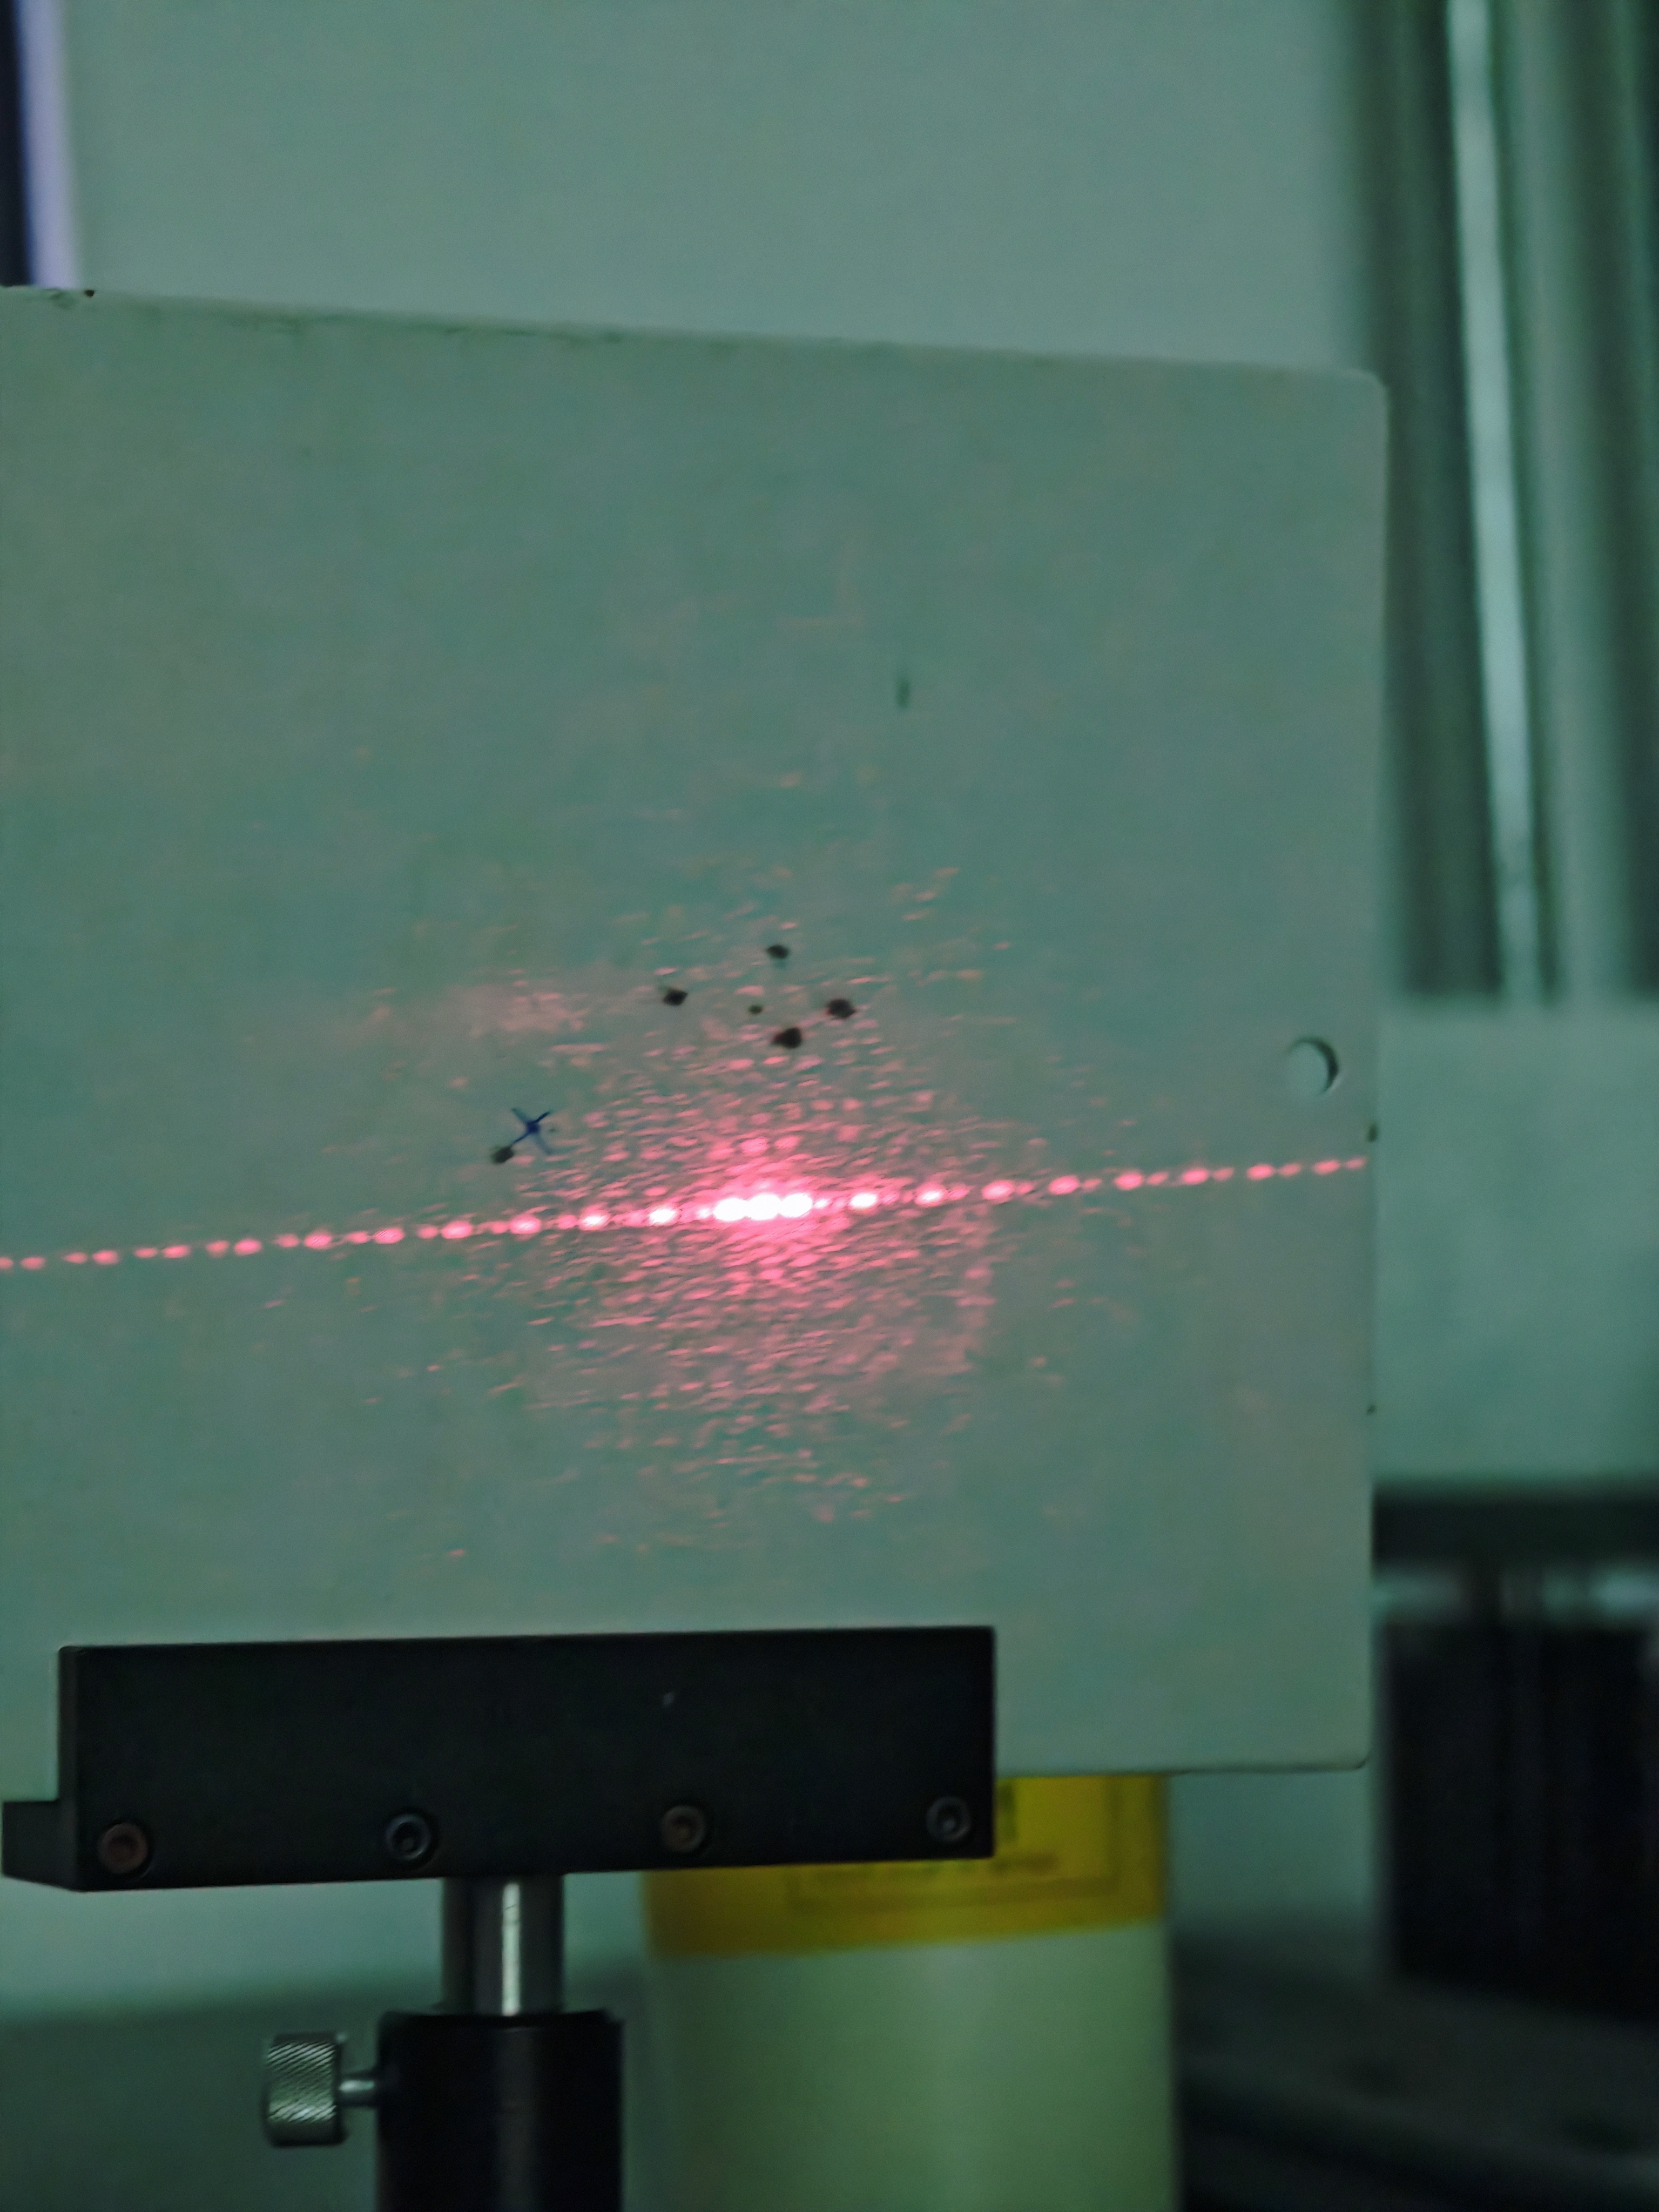
\includegraphics[width=0.24\textwidth]{fig/IMG_20251105_165438.jpg}}
    \caption{夫琅和费衍射与菲涅尔衍射实验结果图1}
\end{figure}

\begin{figure}[htbp]
    \centering
    \subfigure[]{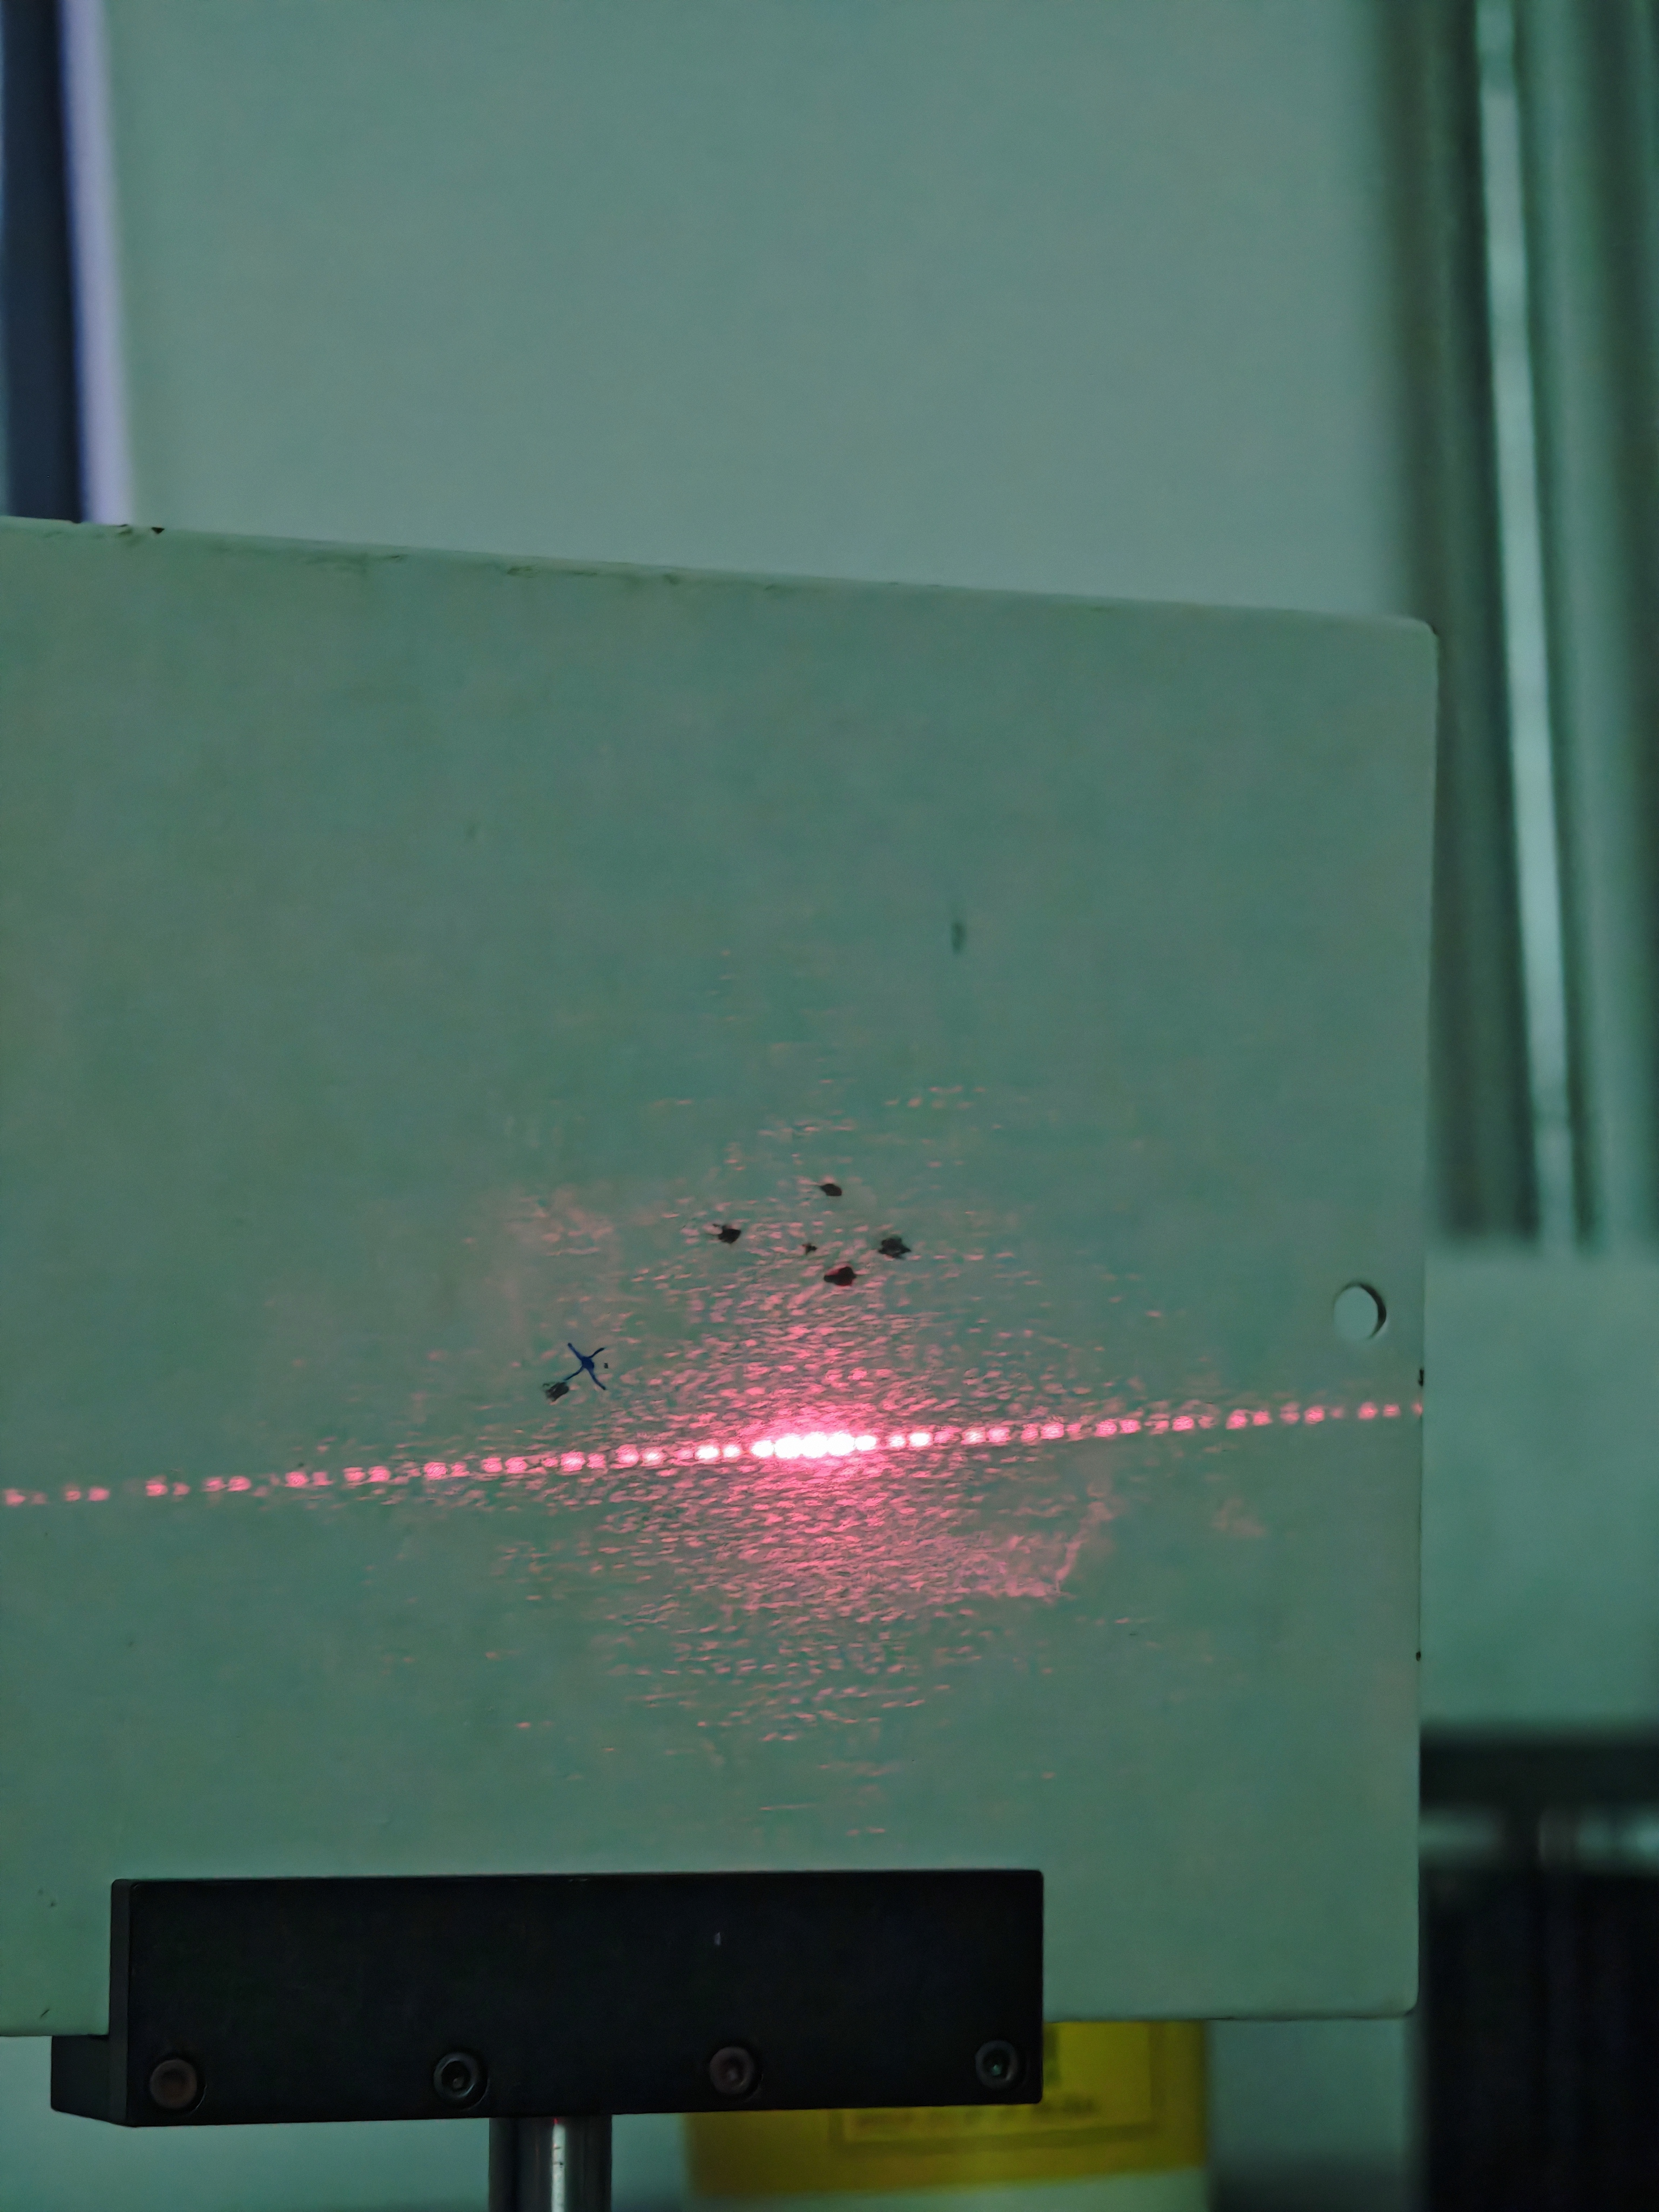
\includegraphics[width=0.24\textwidth]{fig/IMG_20251105_165444.jpg}}
    \subfigure[]{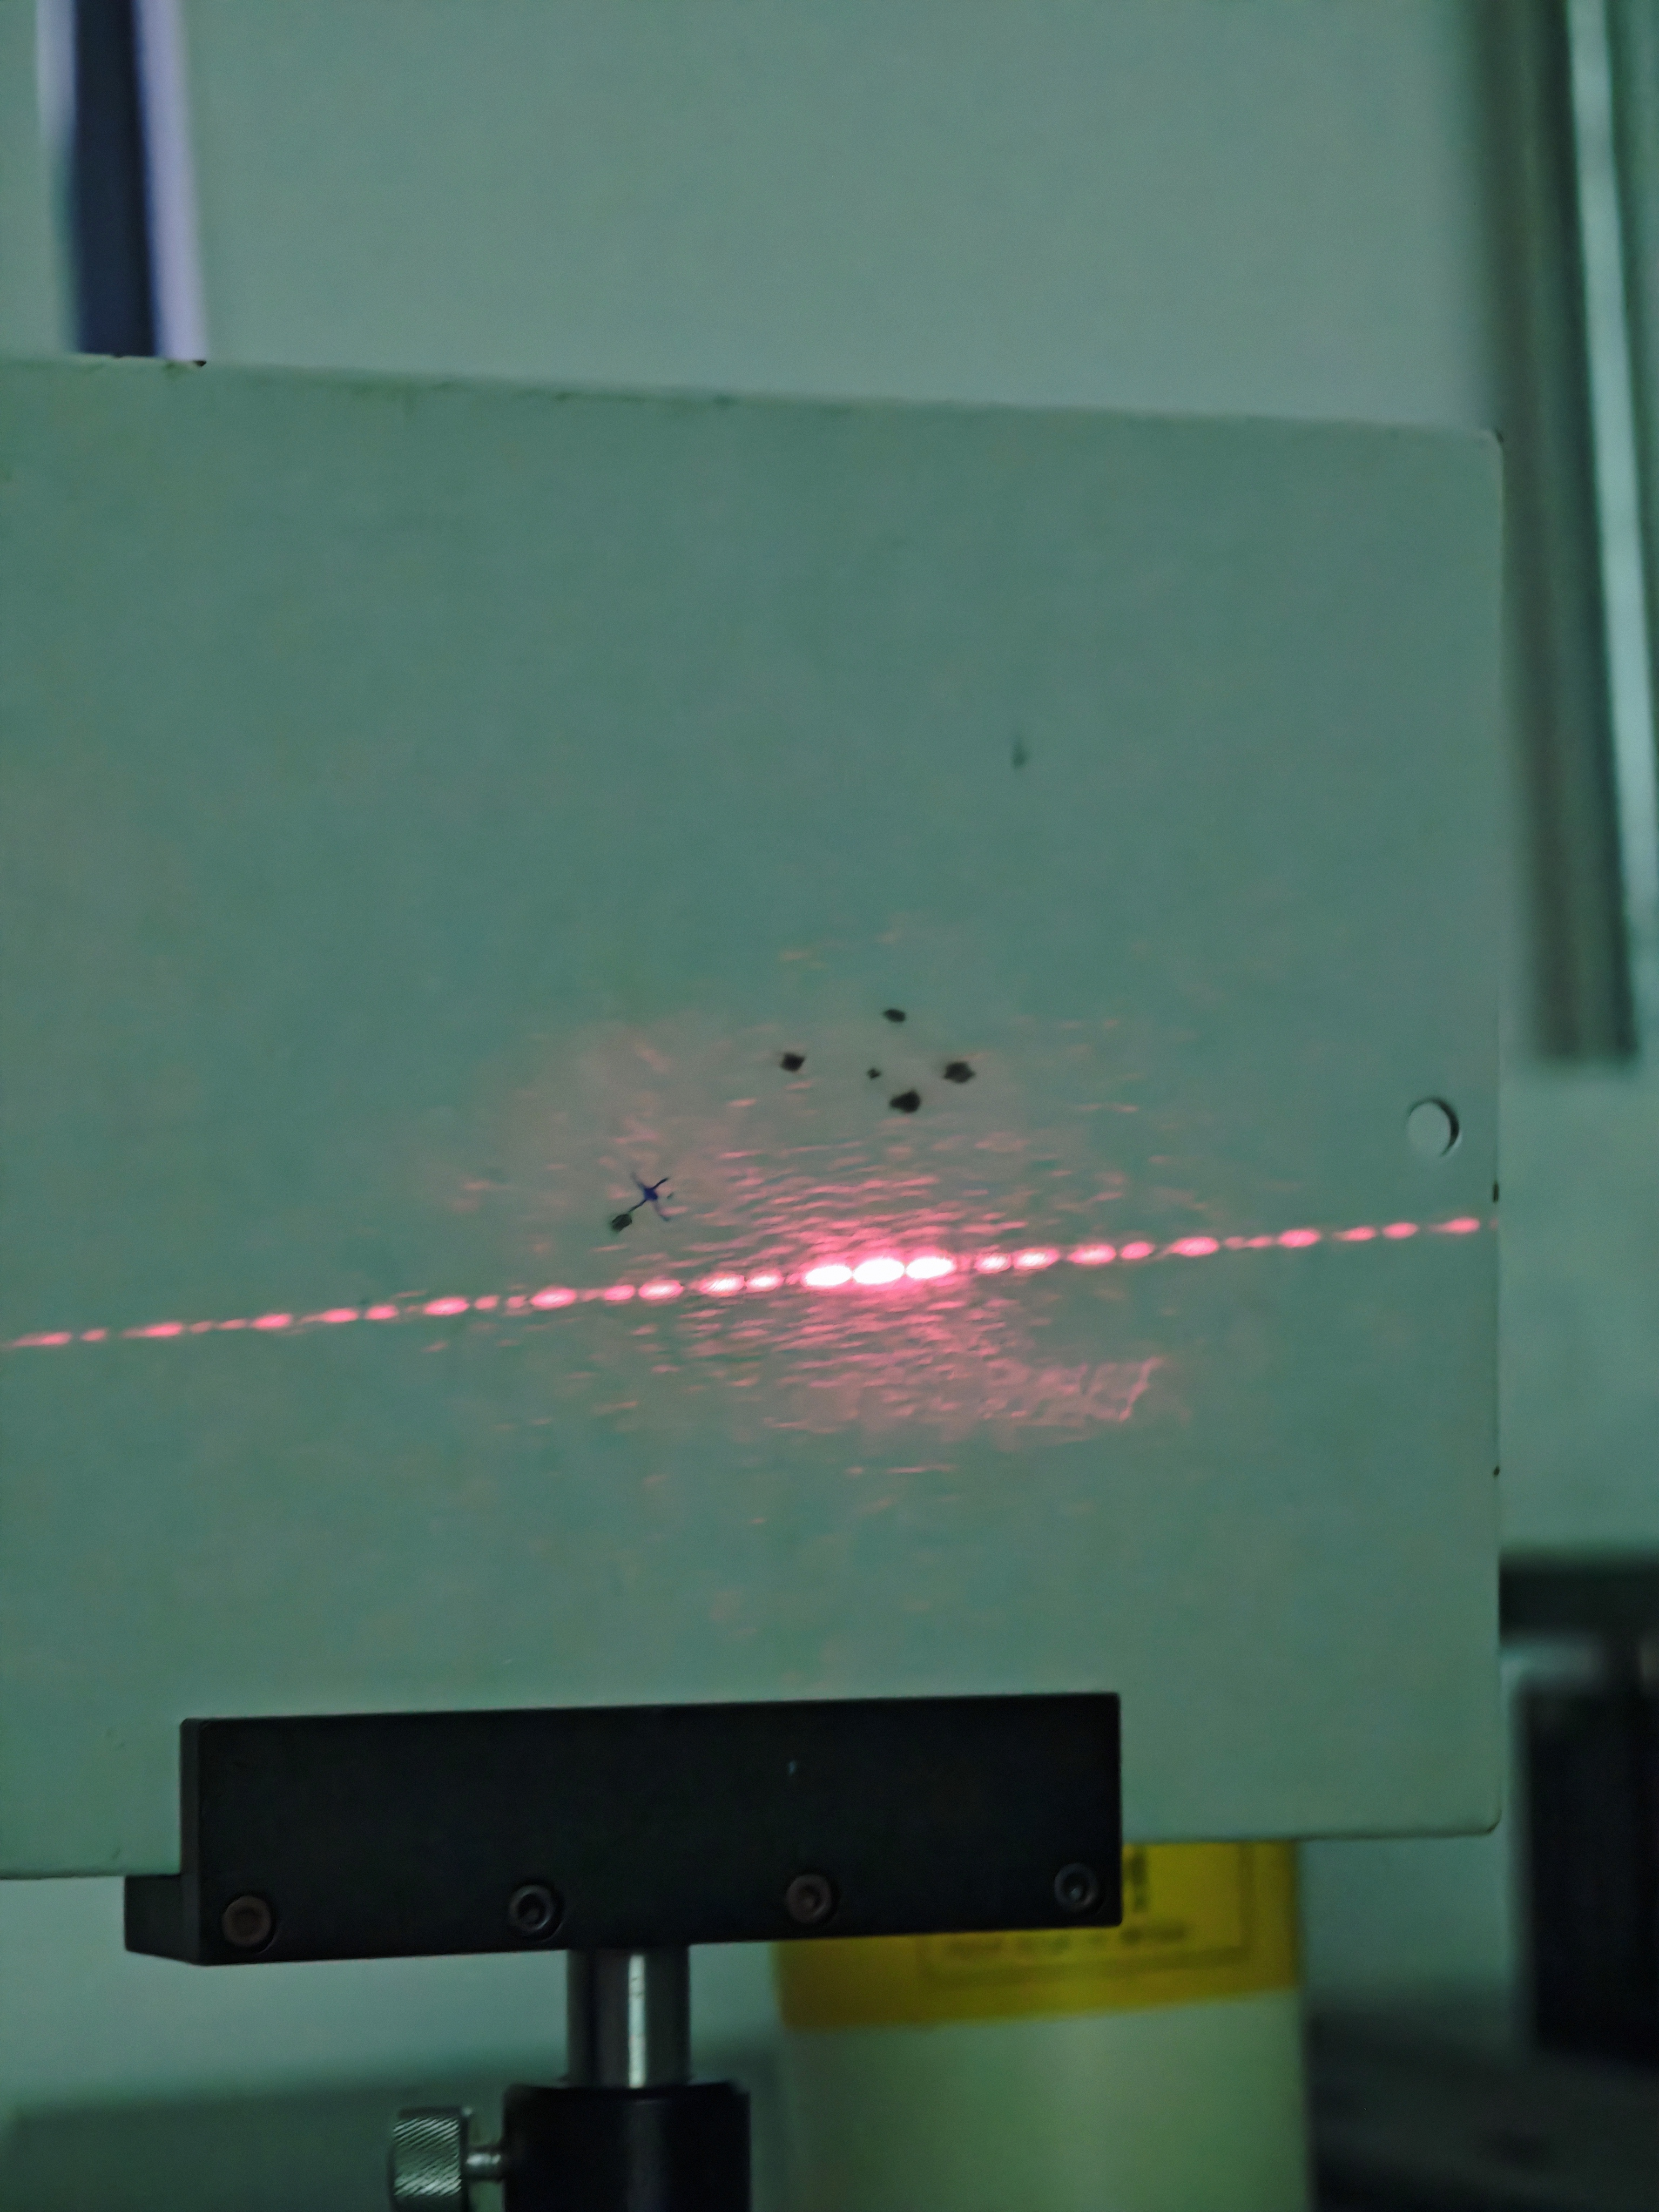
\includegraphics[width=0.24\textwidth]{fig/IMG_20251105_165449.jpg}}
    \subfigure[]{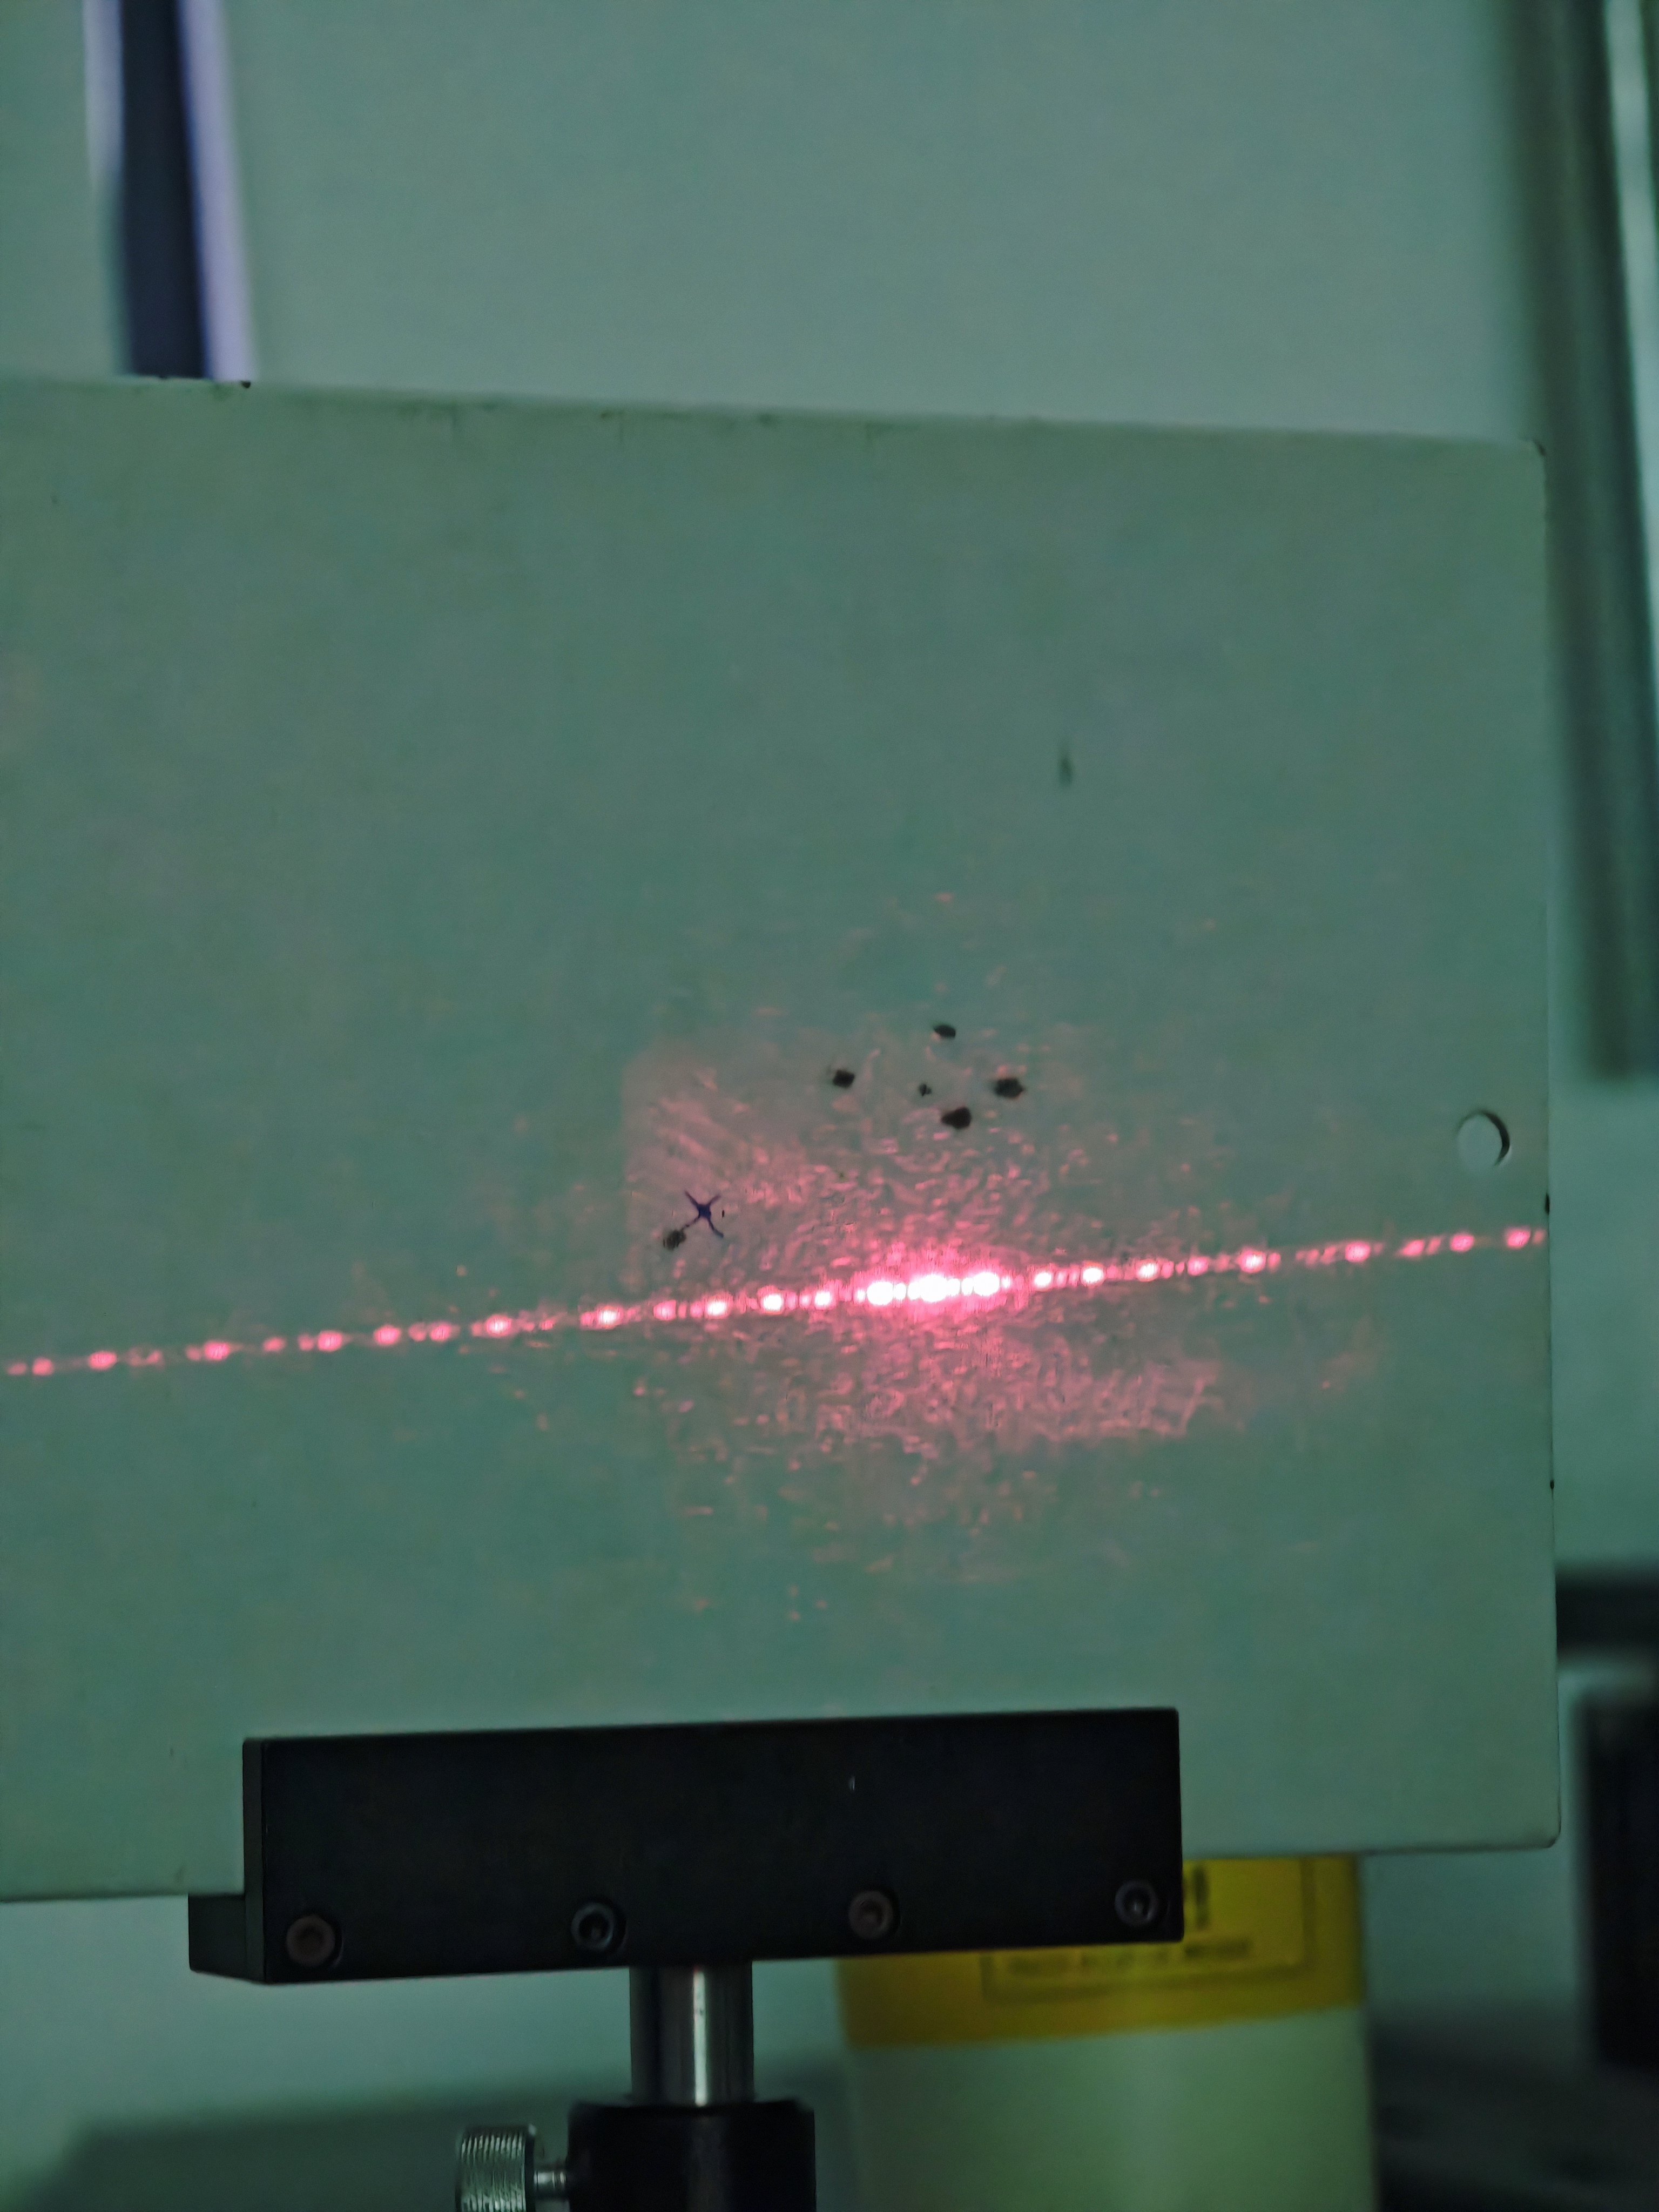
\includegraphics[width=0.24\textwidth]{fig/IMG_20251105_165455.jpg}}
    \subfigure[]{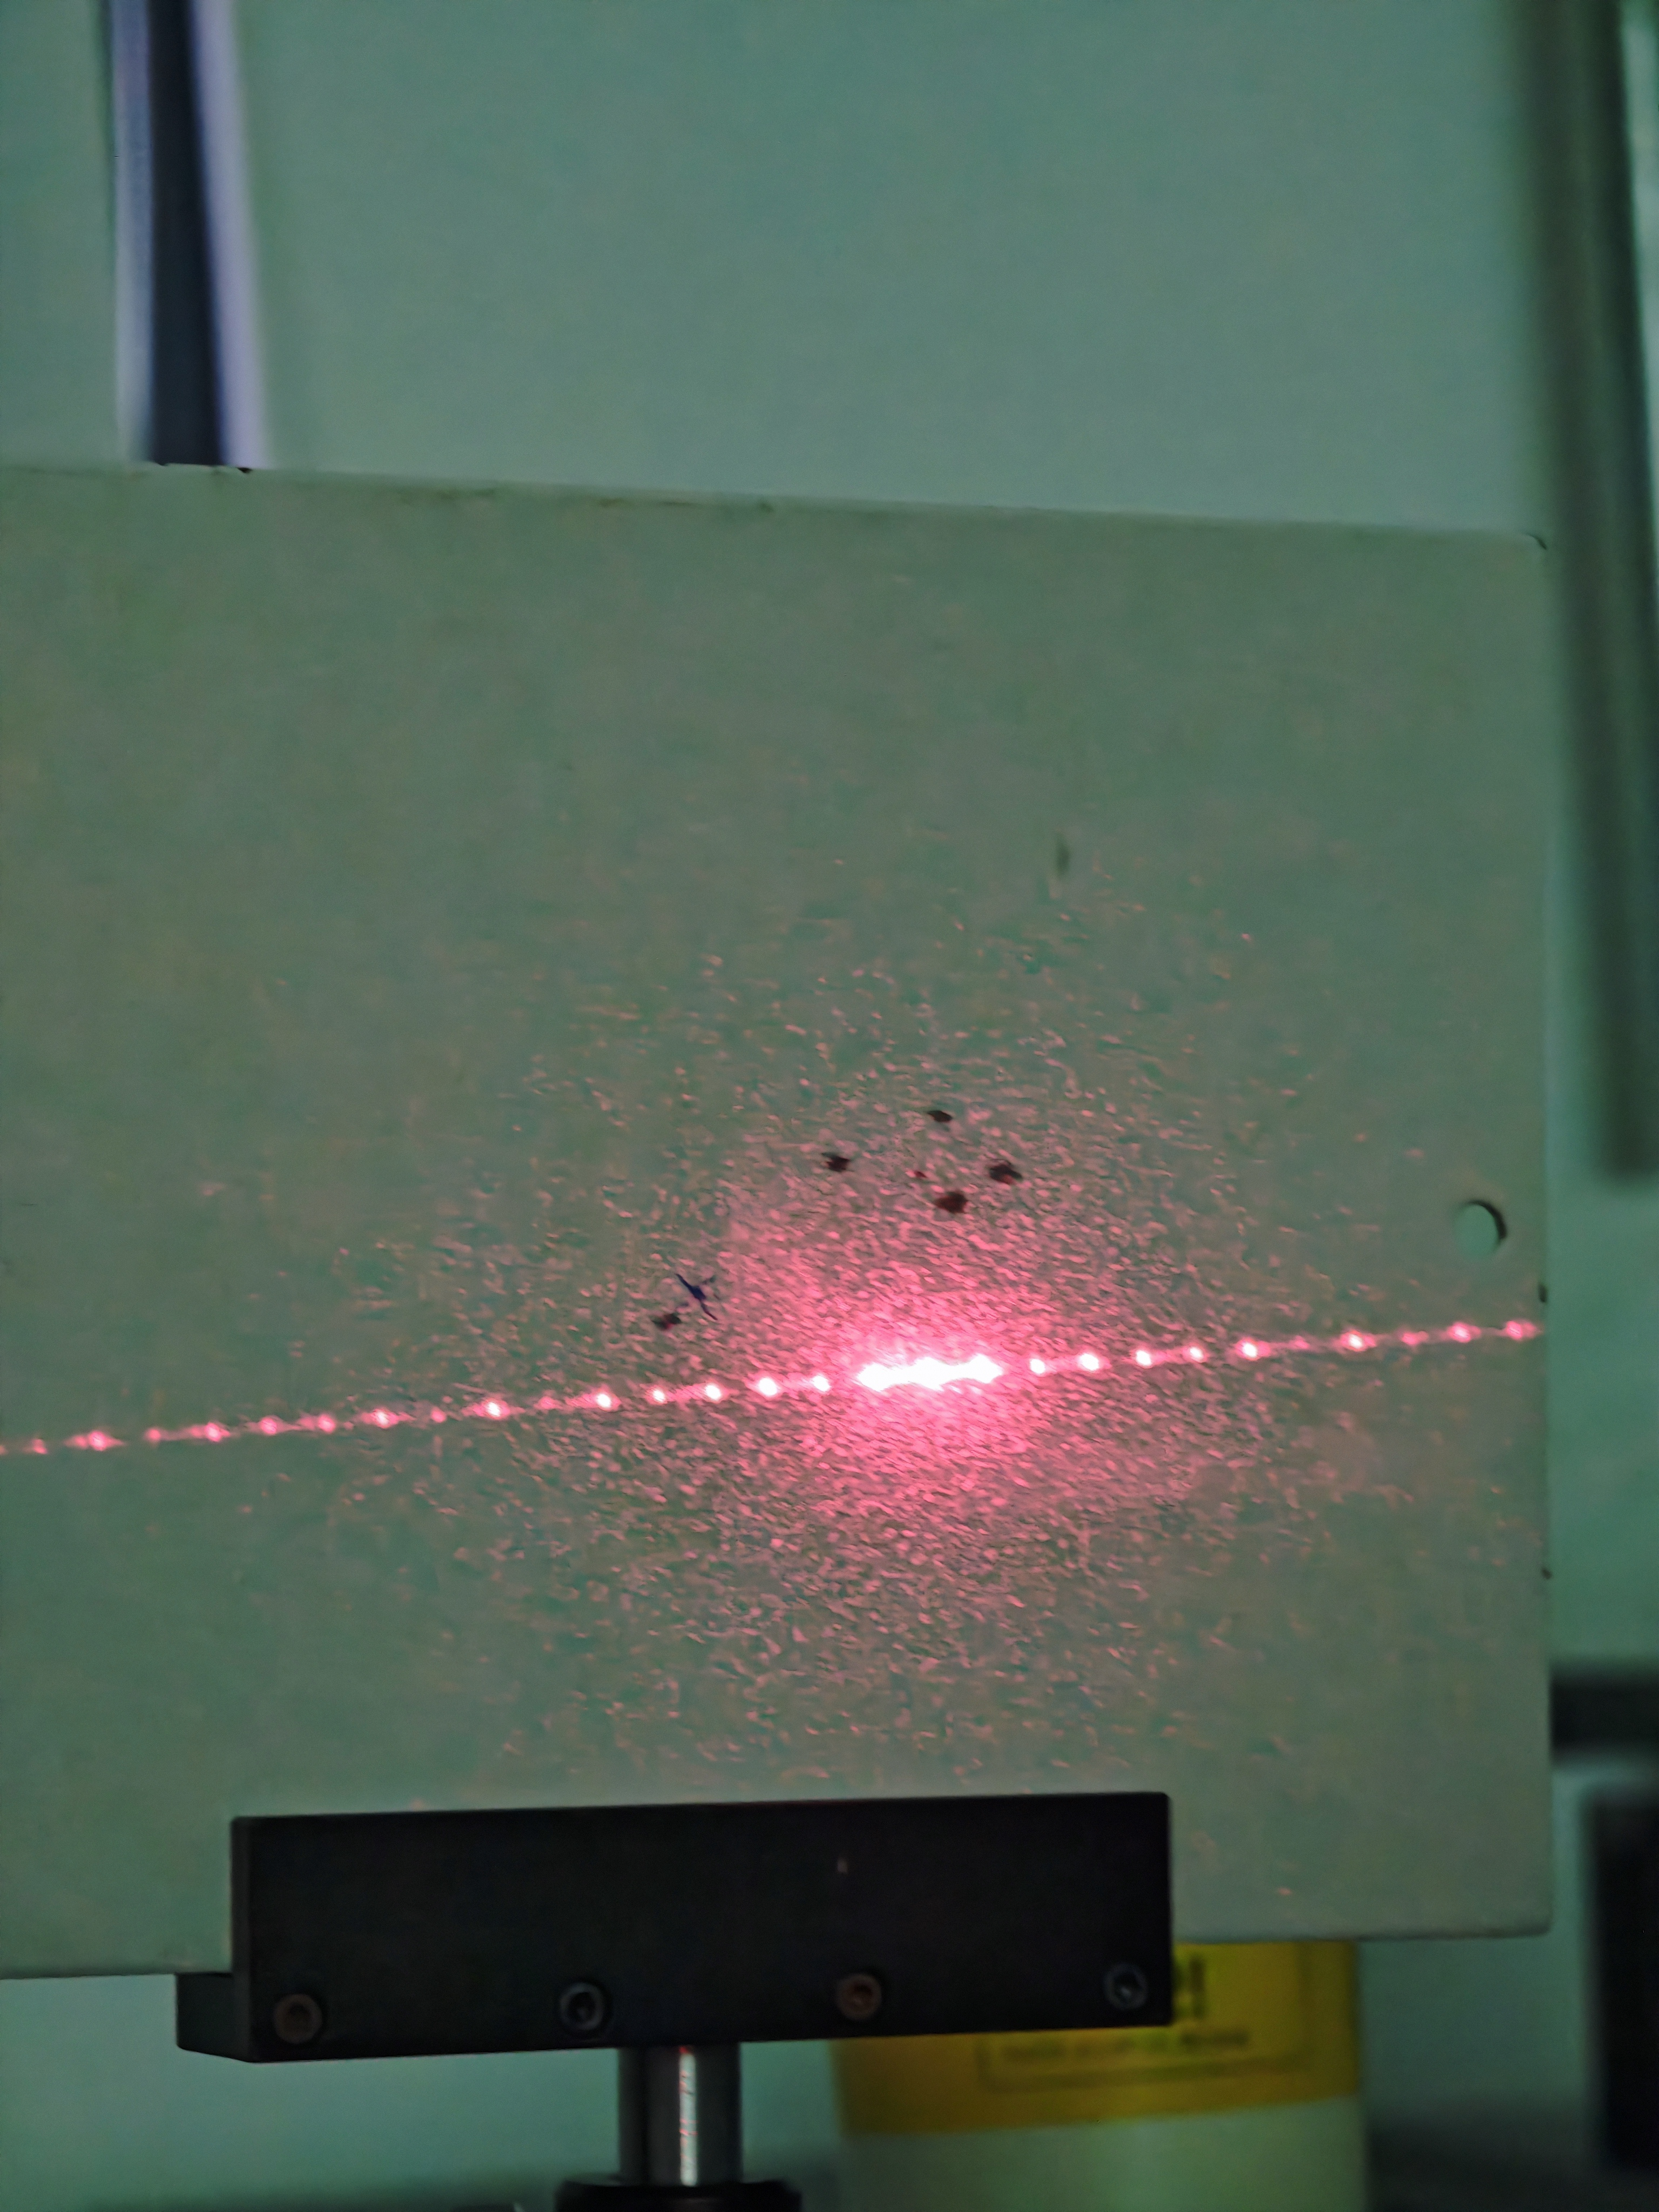
\includegraphics[width=0.24\textwidth]{fig/IMG_20251105_165501.jpg}}
    \subfigure[]{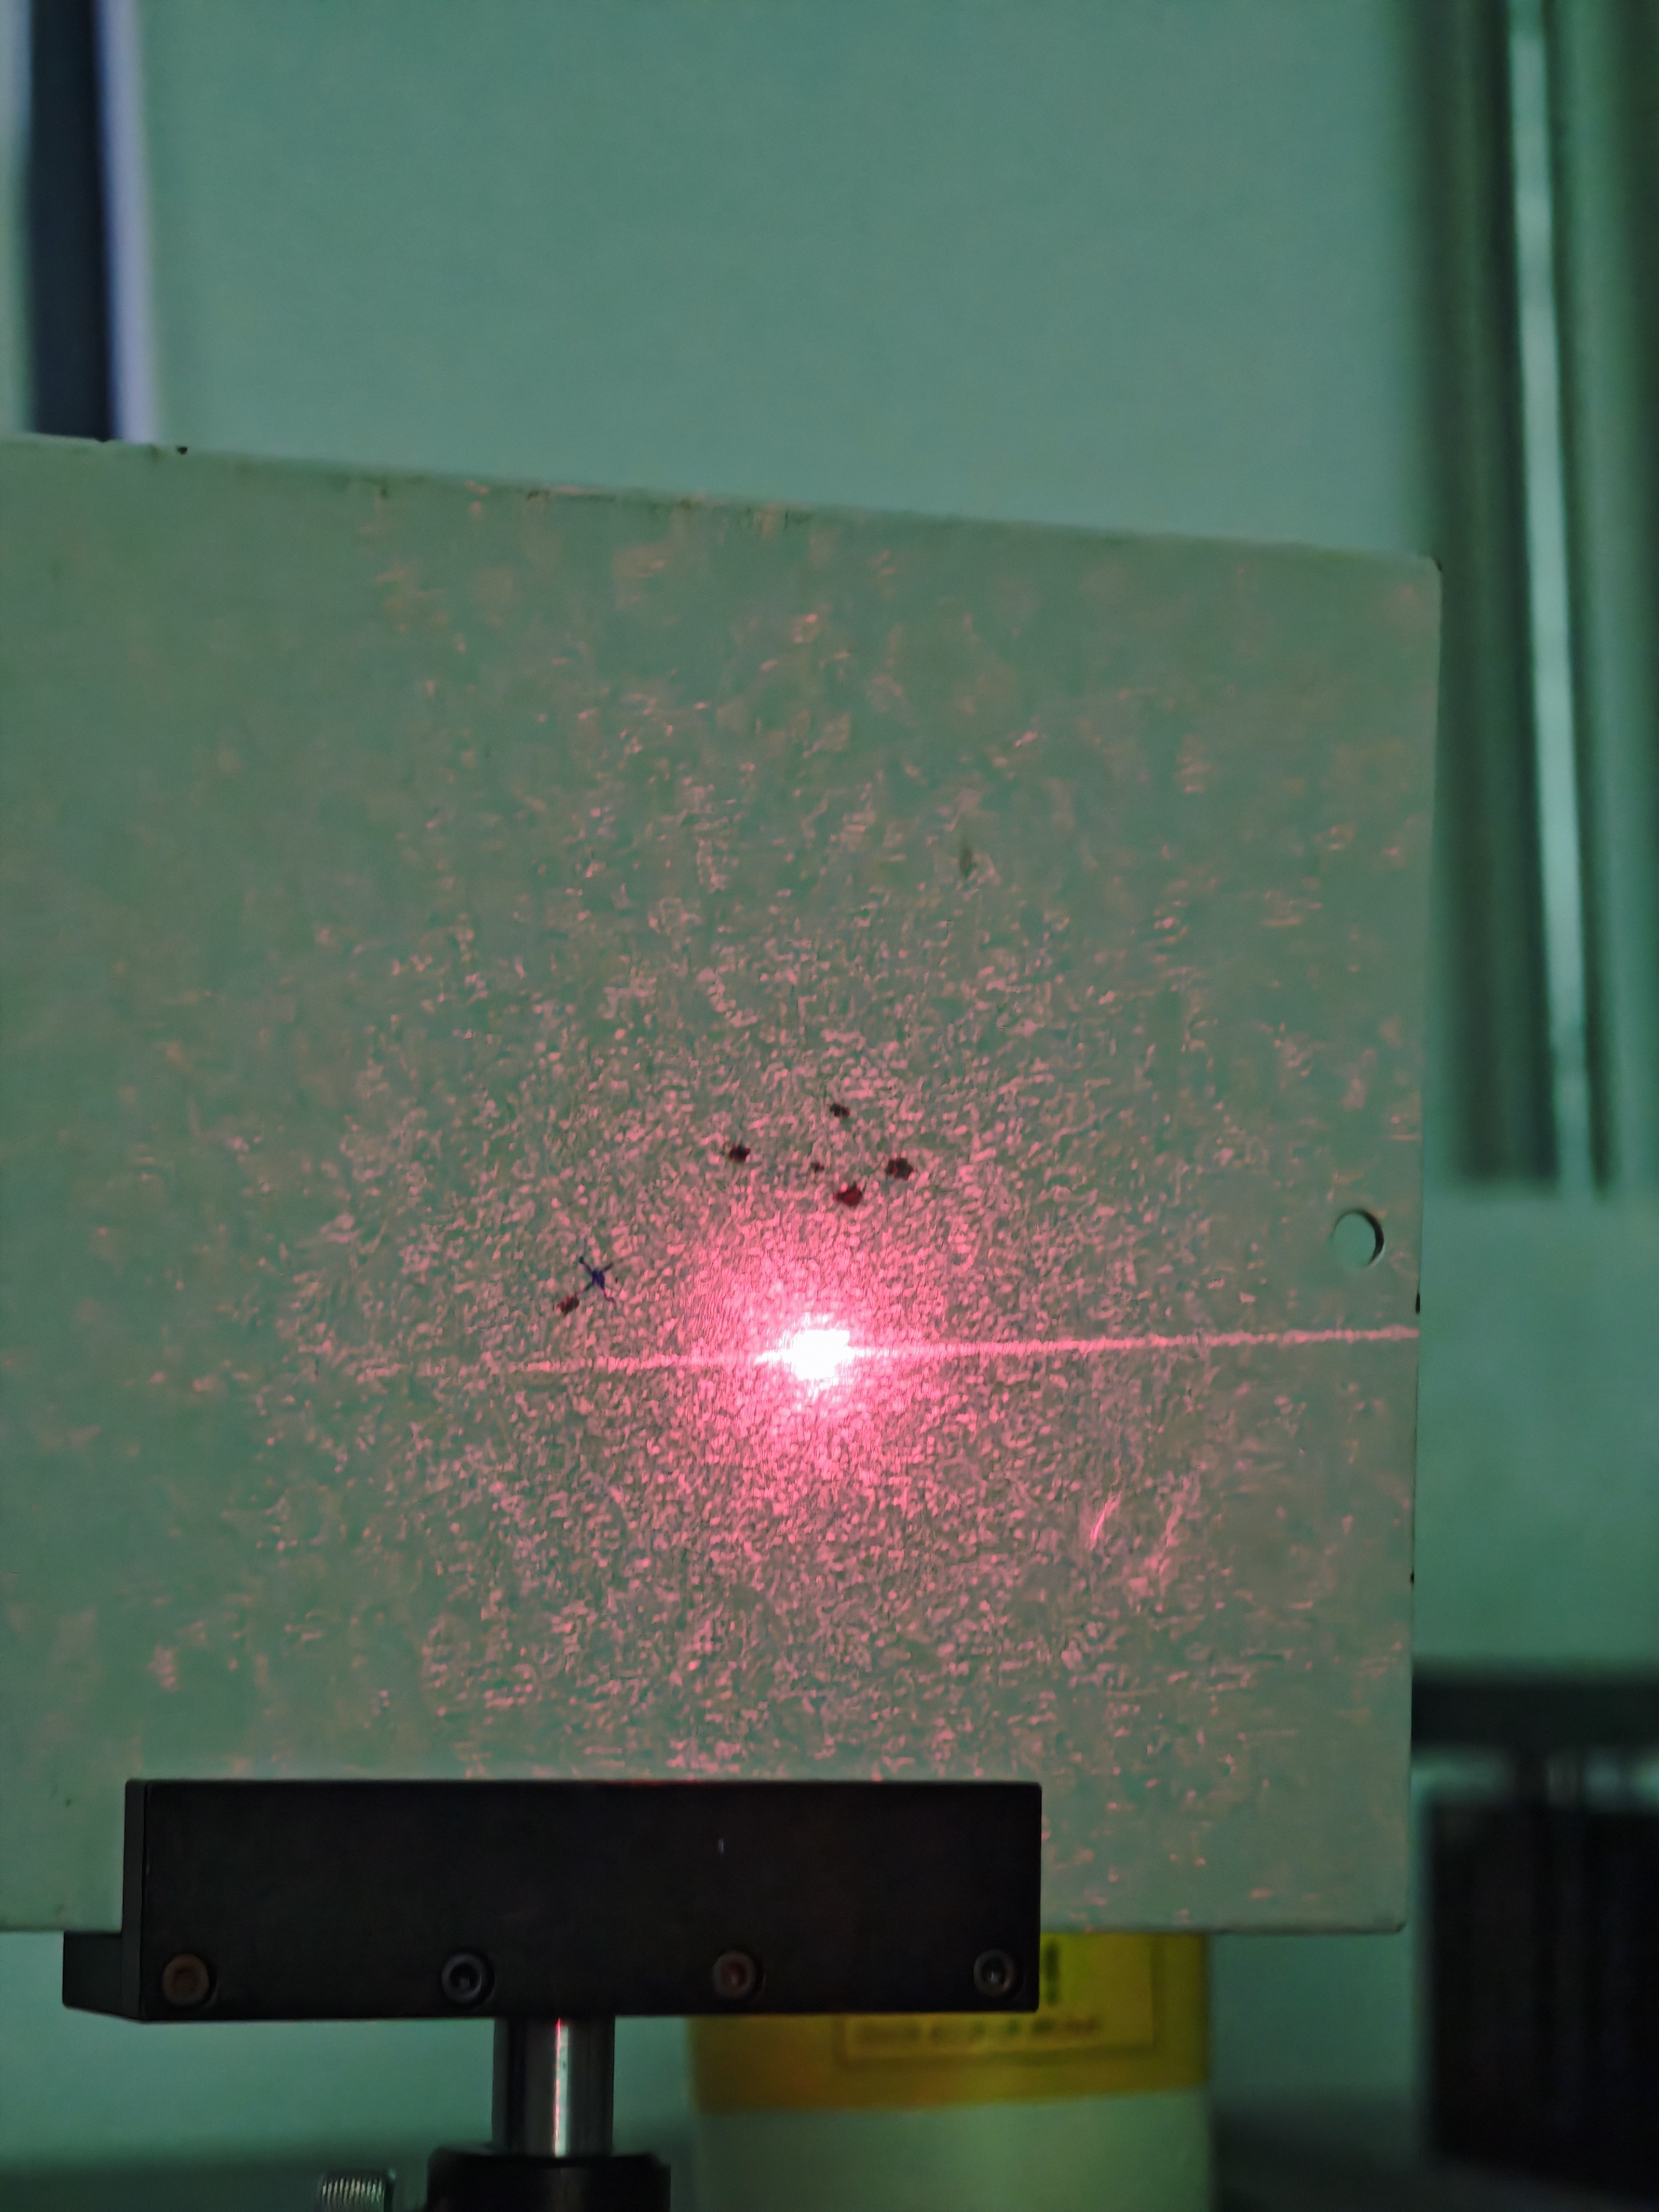
\includegraphics[width=0.24\textwidth]{fig/IMG_20251105_165655.jpg}}
    \subfigure[]{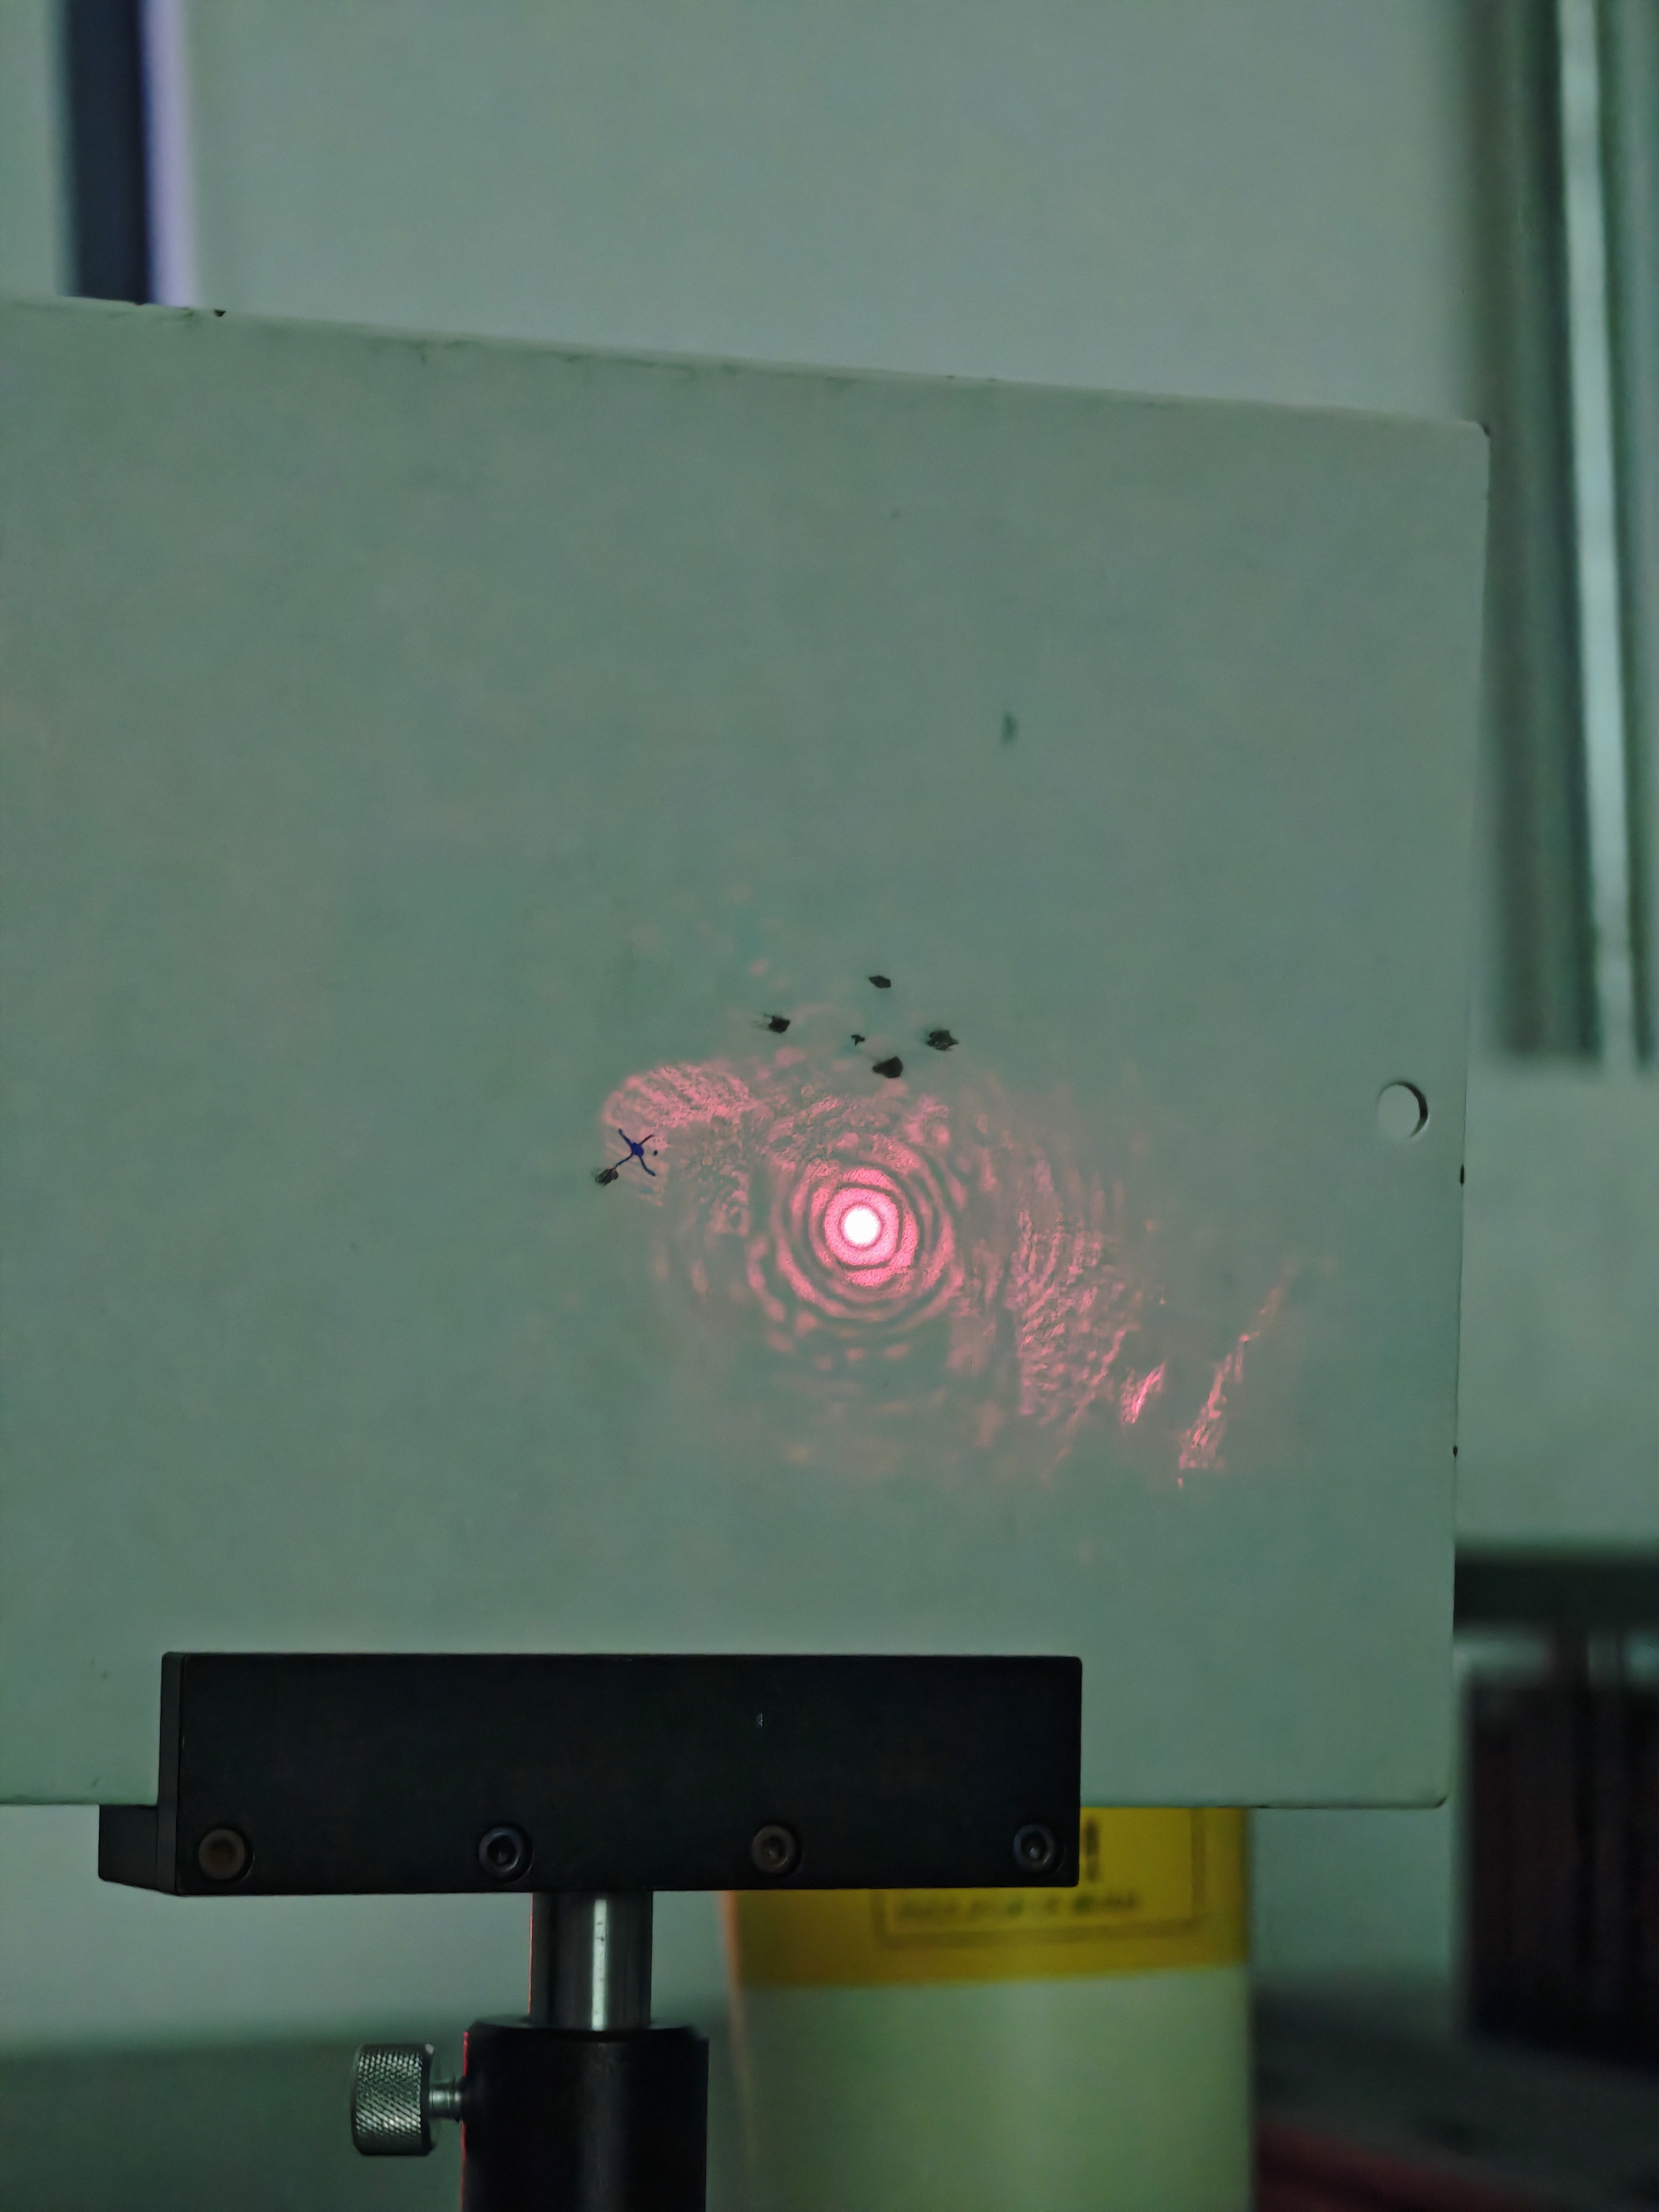
\includegraphics[width=0.24\textwidth]{fig/IMG_20251105_165703.jpg}}
    \subfigure[]{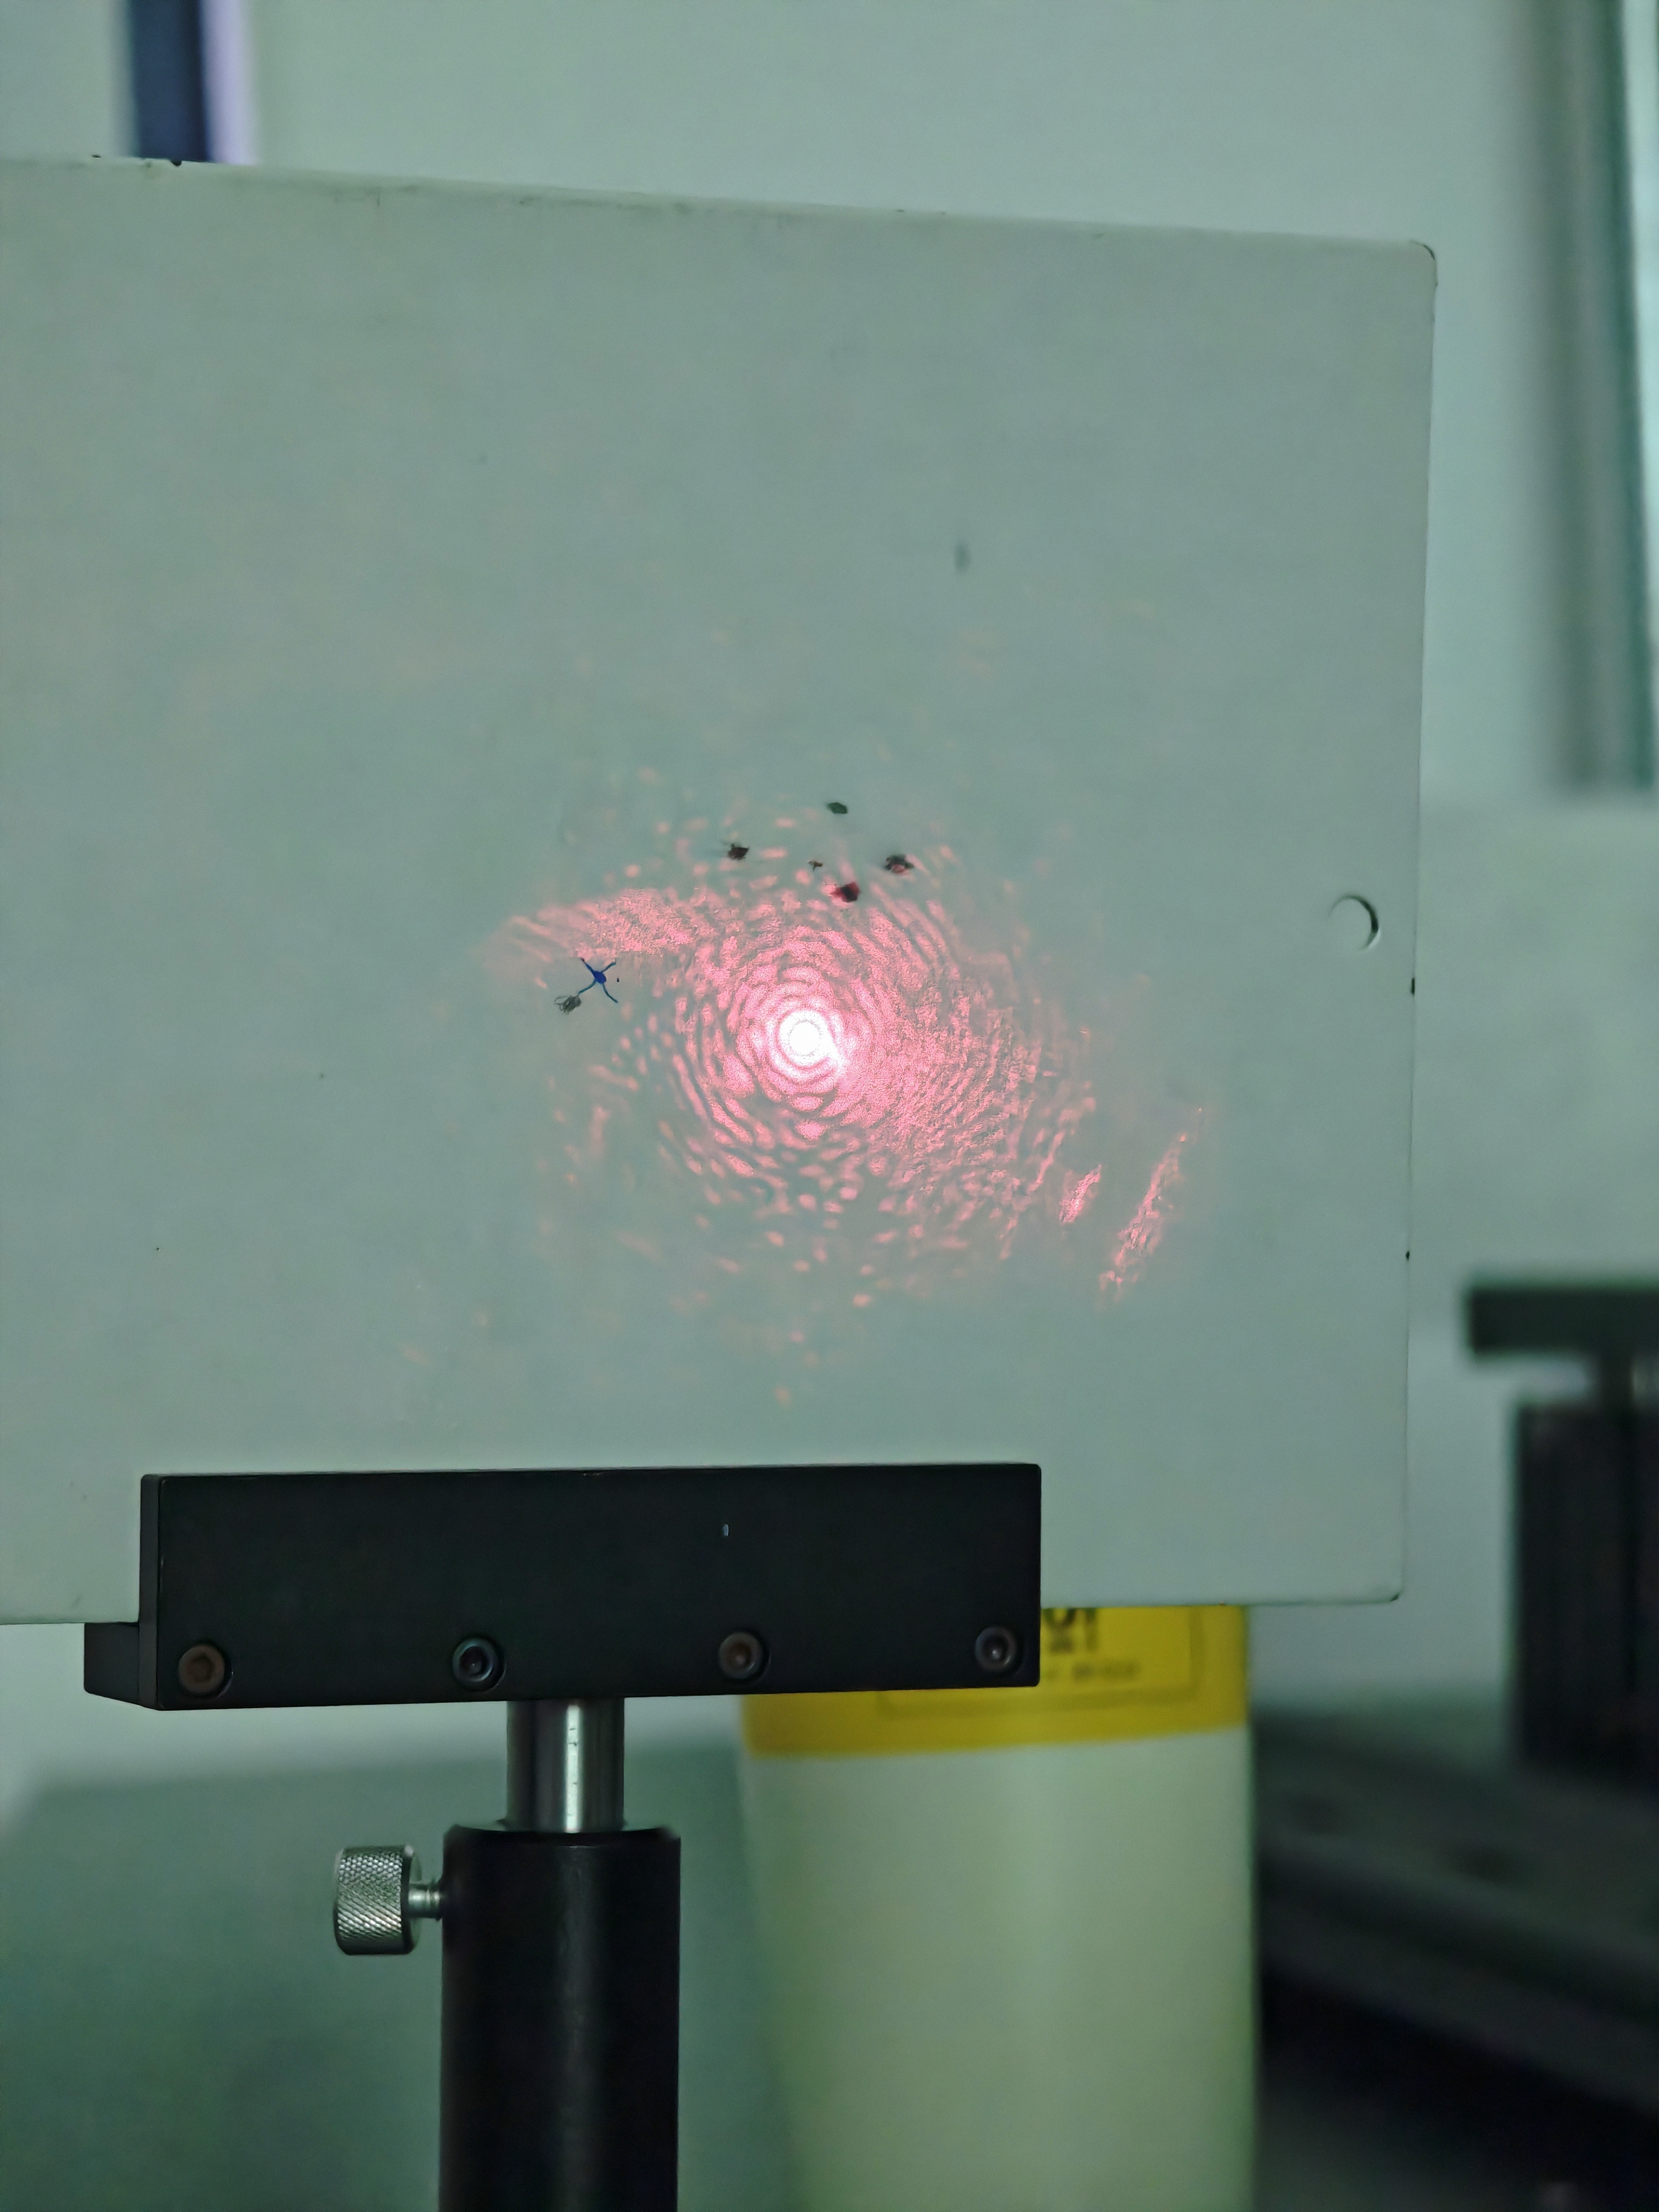
\includegraphics[width=0.24\textwidth]{fig/IMG_20251105_165722.jpg}}
    \subfigure[]{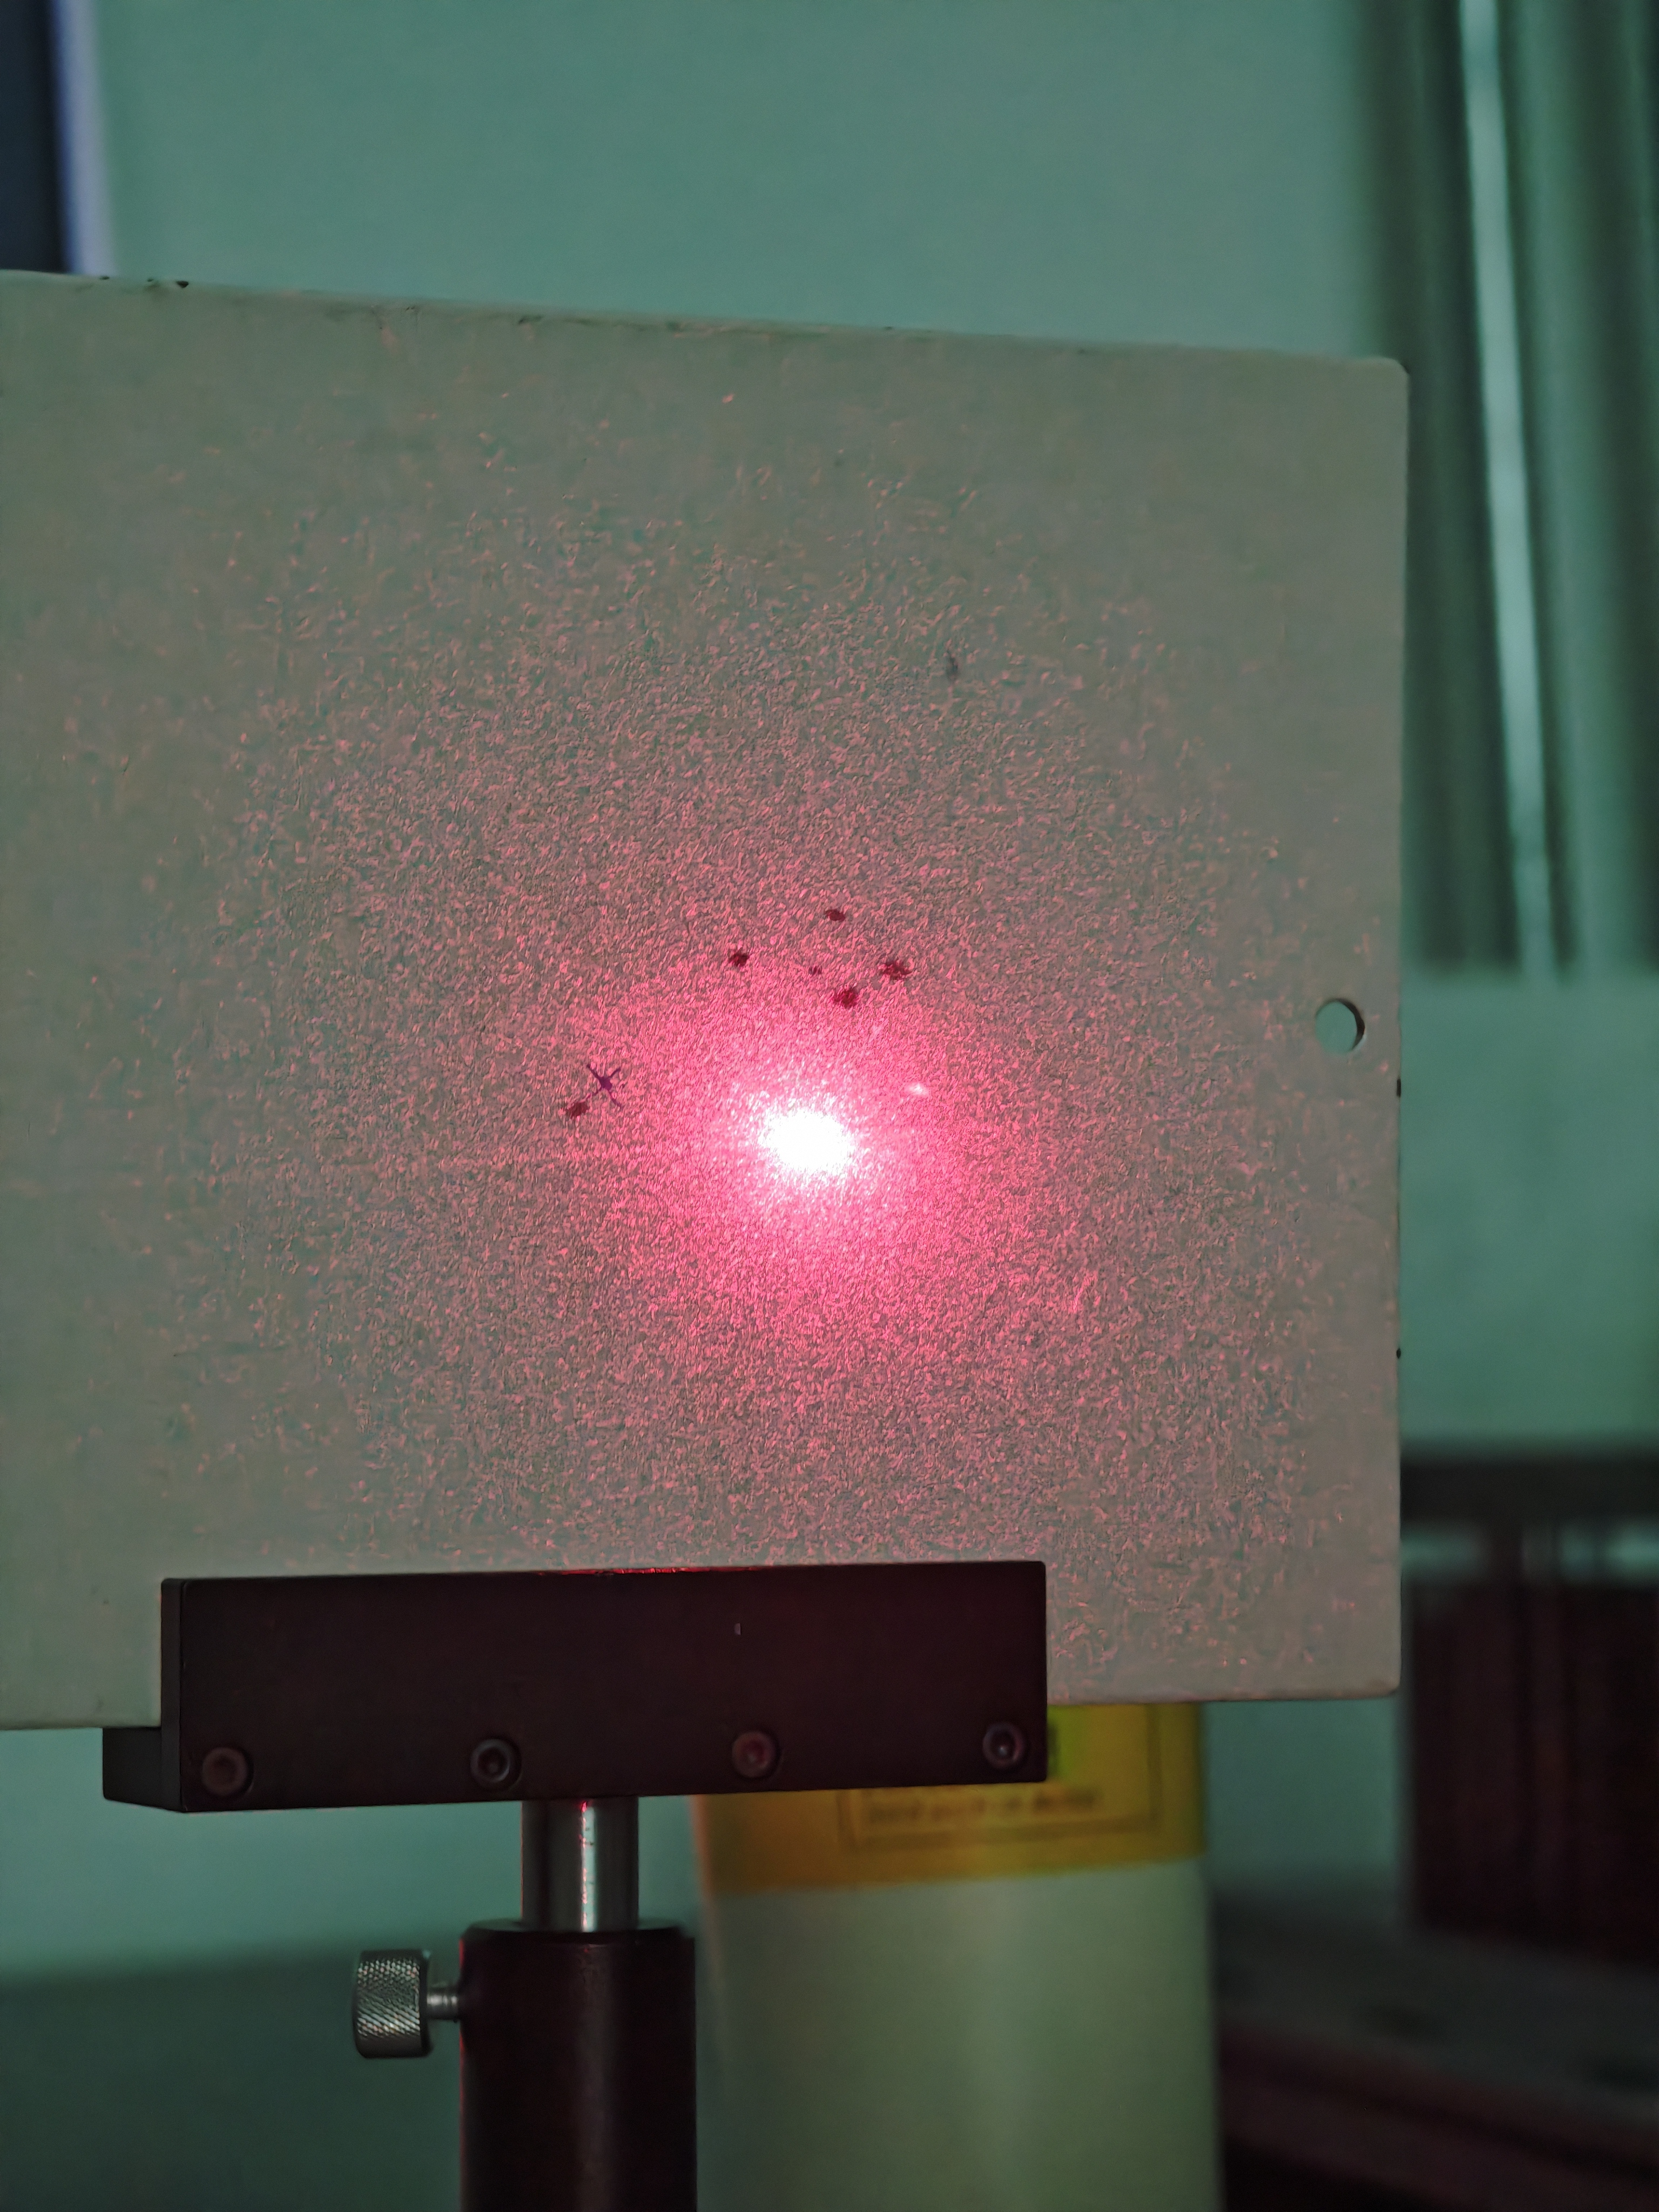
\includegraphics[width=0.24\textwidth]{fig/IMG_20251105_165755.jpg}}
    \caption{夫琅和费衍射与菲涅尔衍射实验结果图2}
\end{figure}

\begin{figure}[htbp]
    \centering
    \subfigure[]{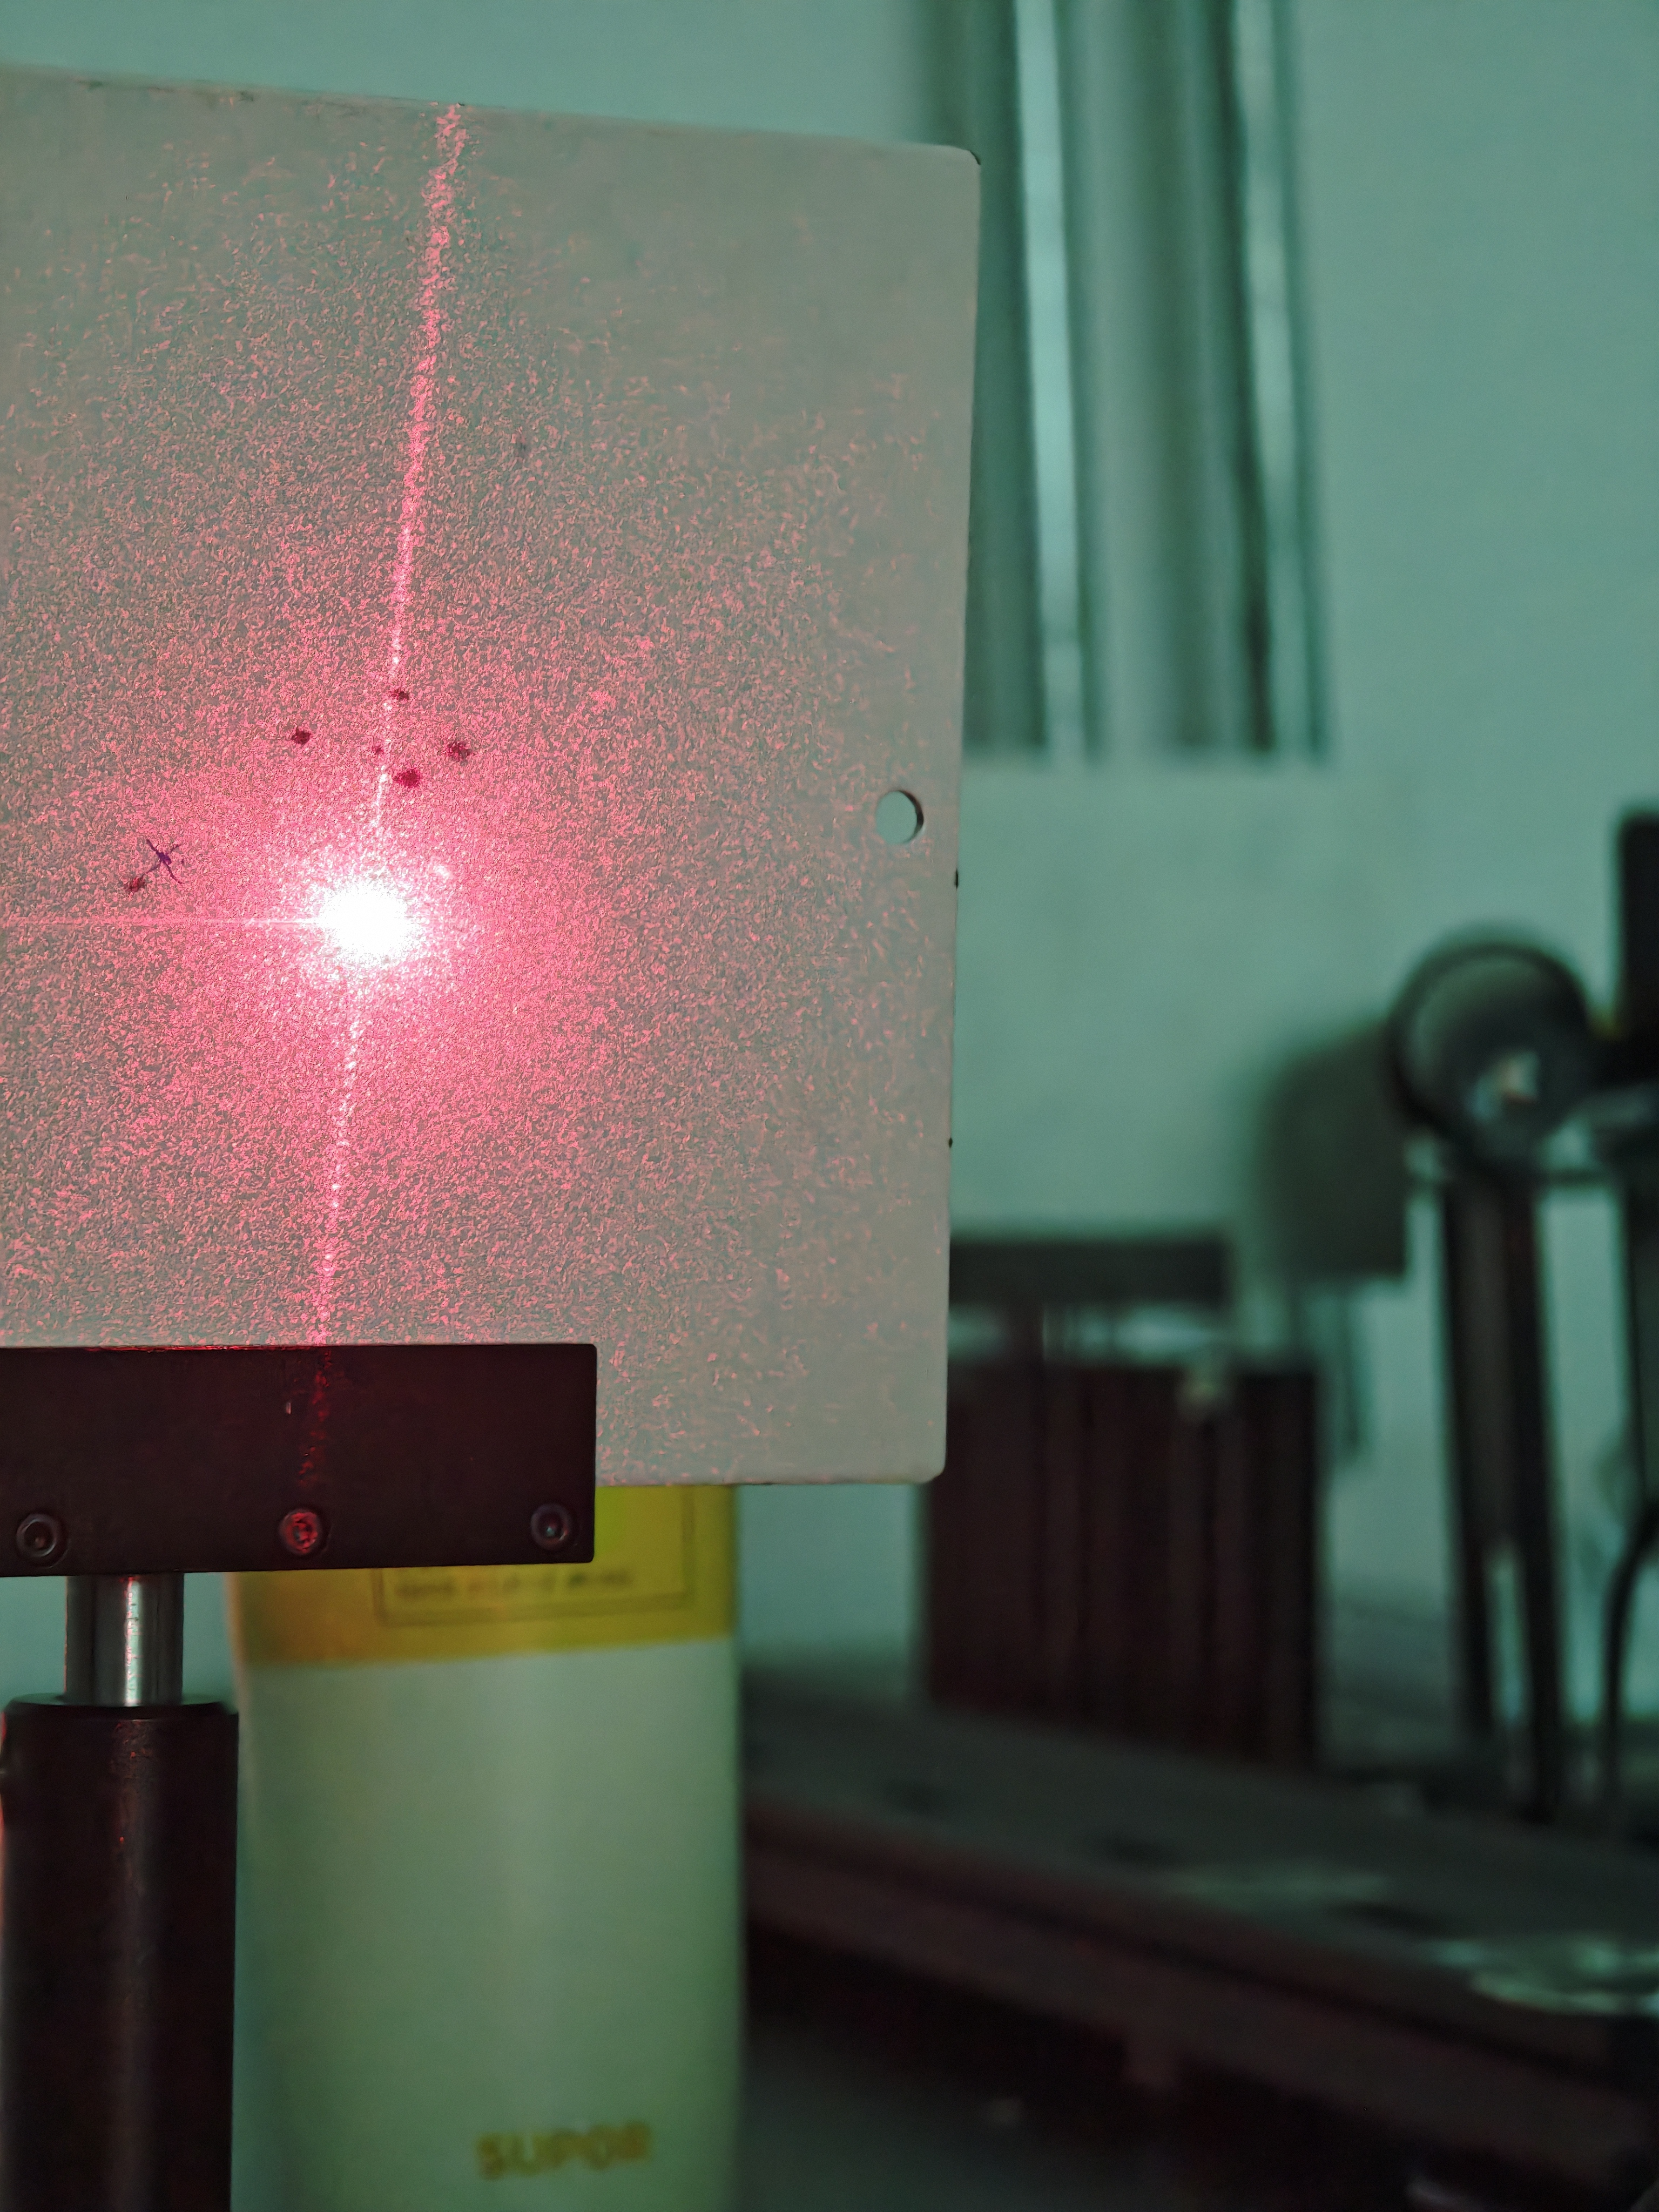
\includegraphics[width=0.24\textwidth]{fig/IMG_20251105_165809.jpg}}
    \subfigure[]{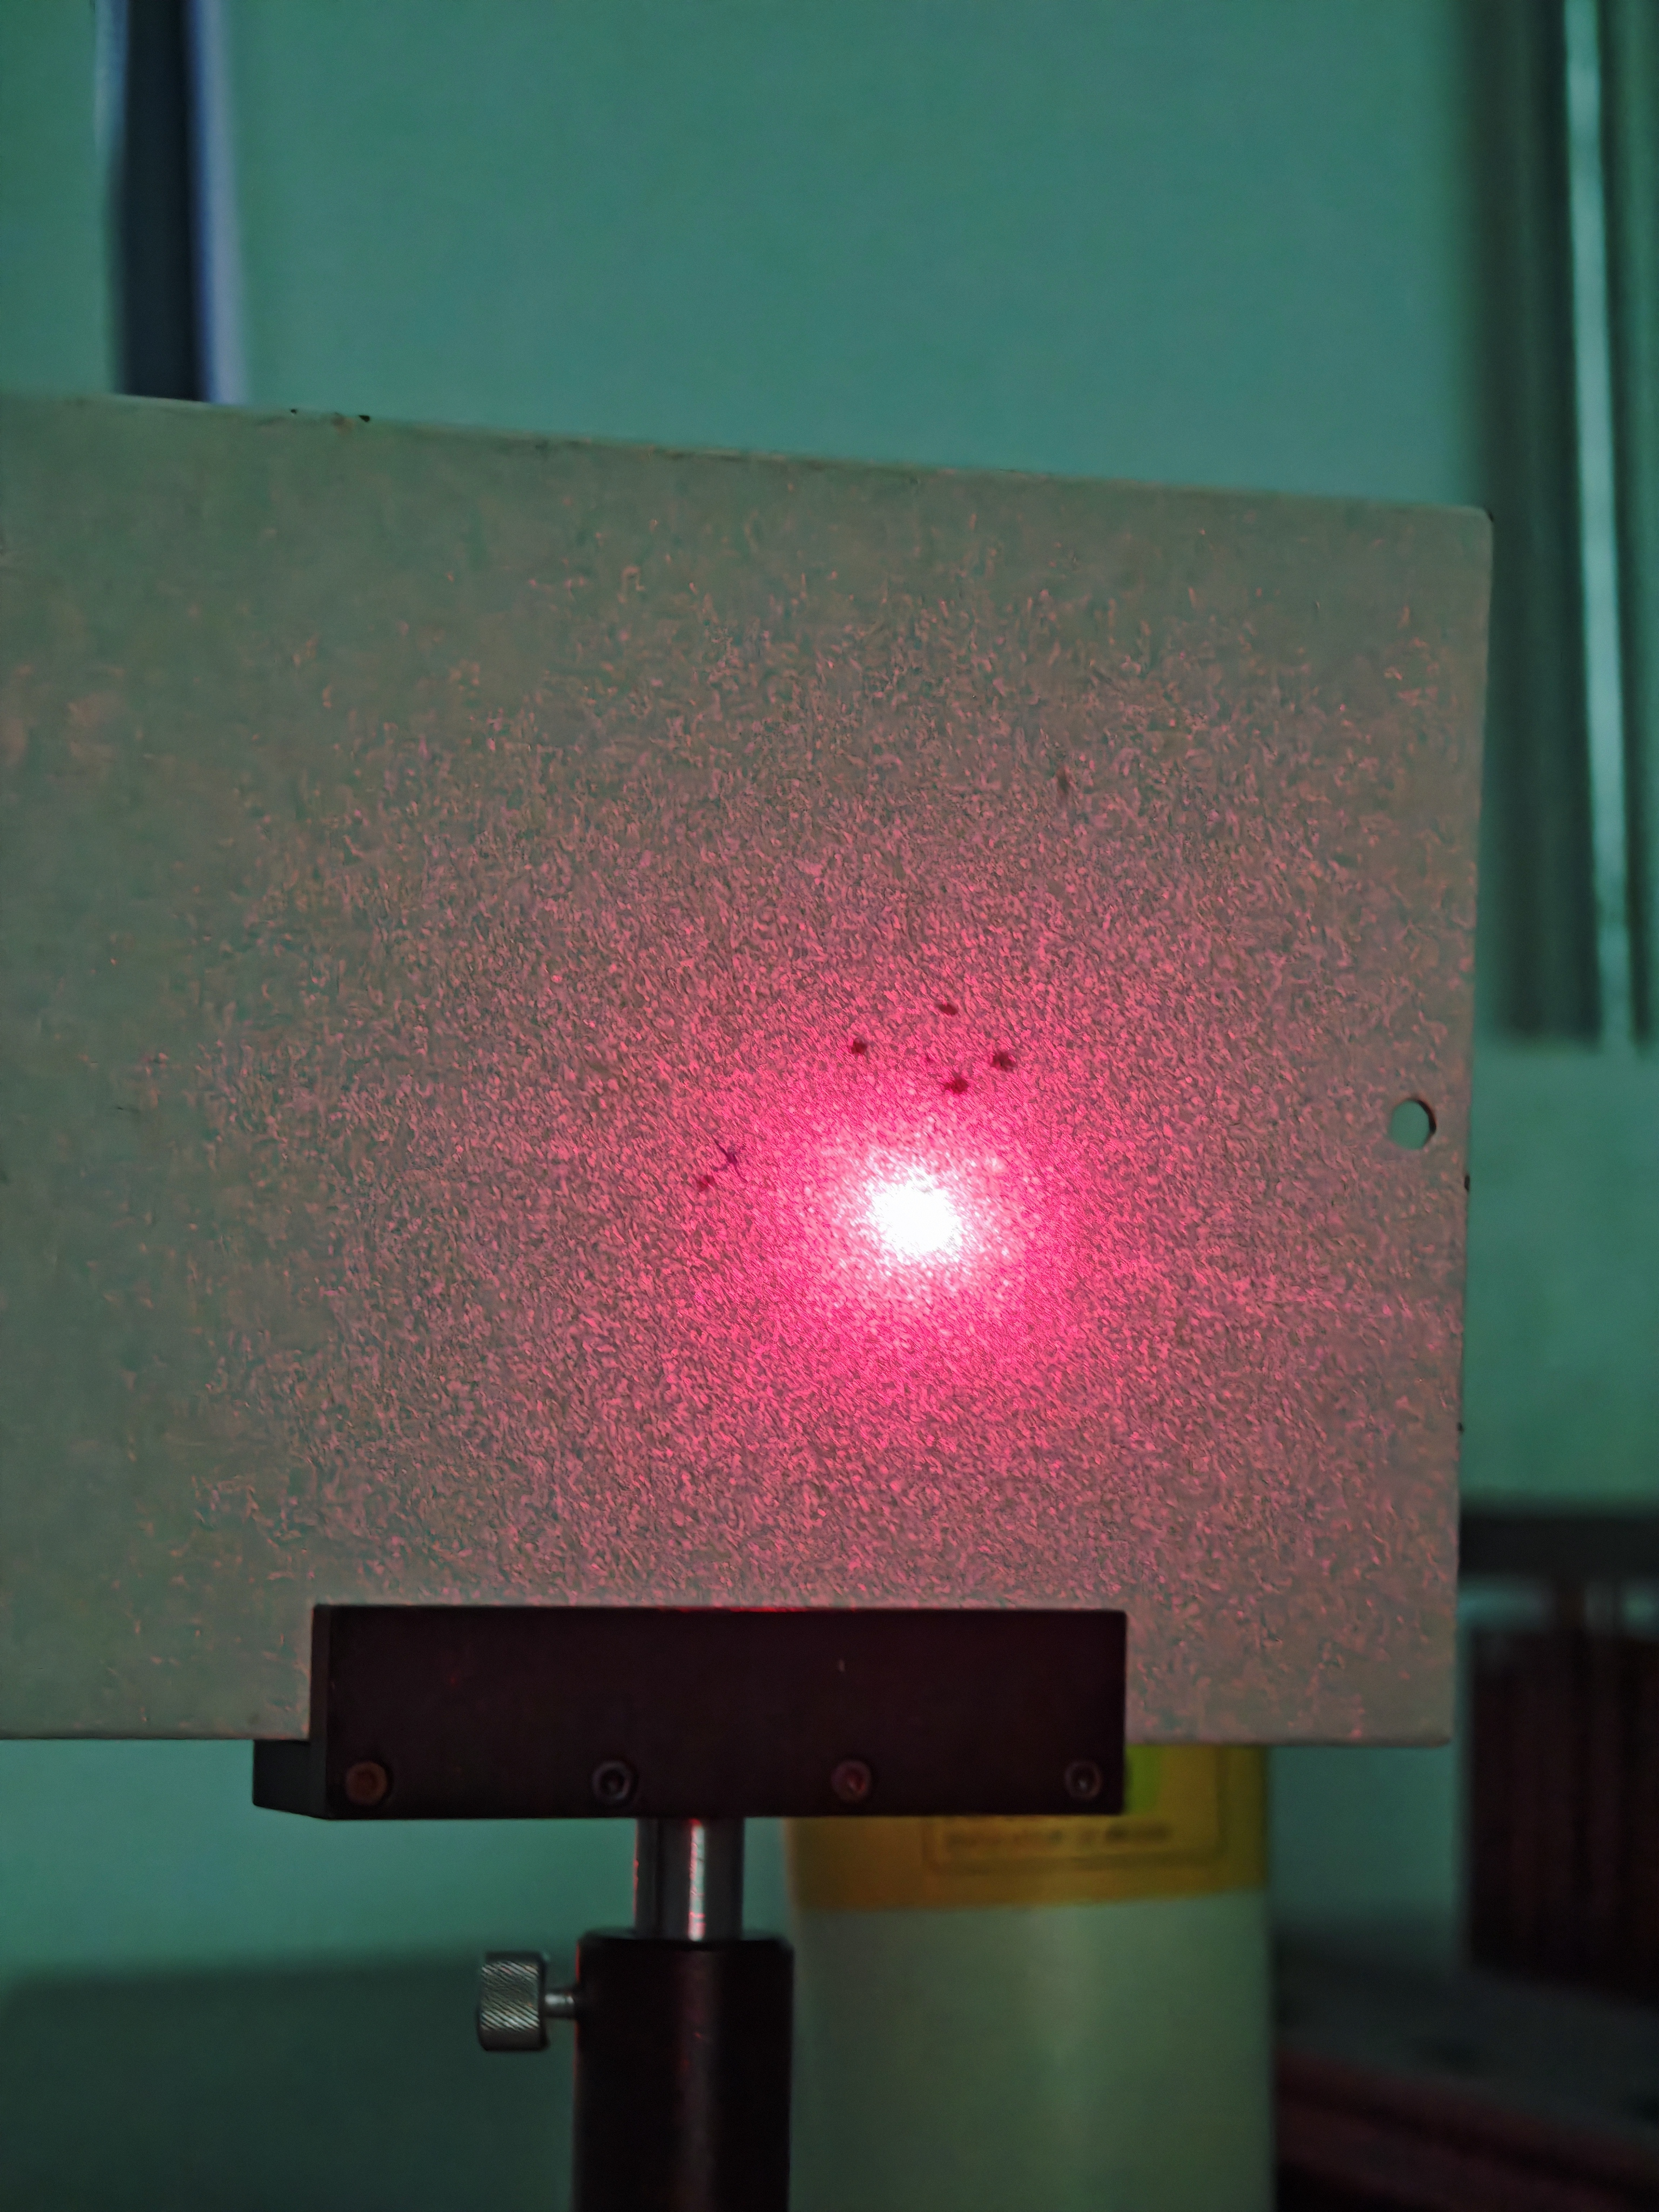
\includegraphics[width=0.24\textwidth]{fig/IMG_20251105_165843.jpg}}
    \subfigure[]{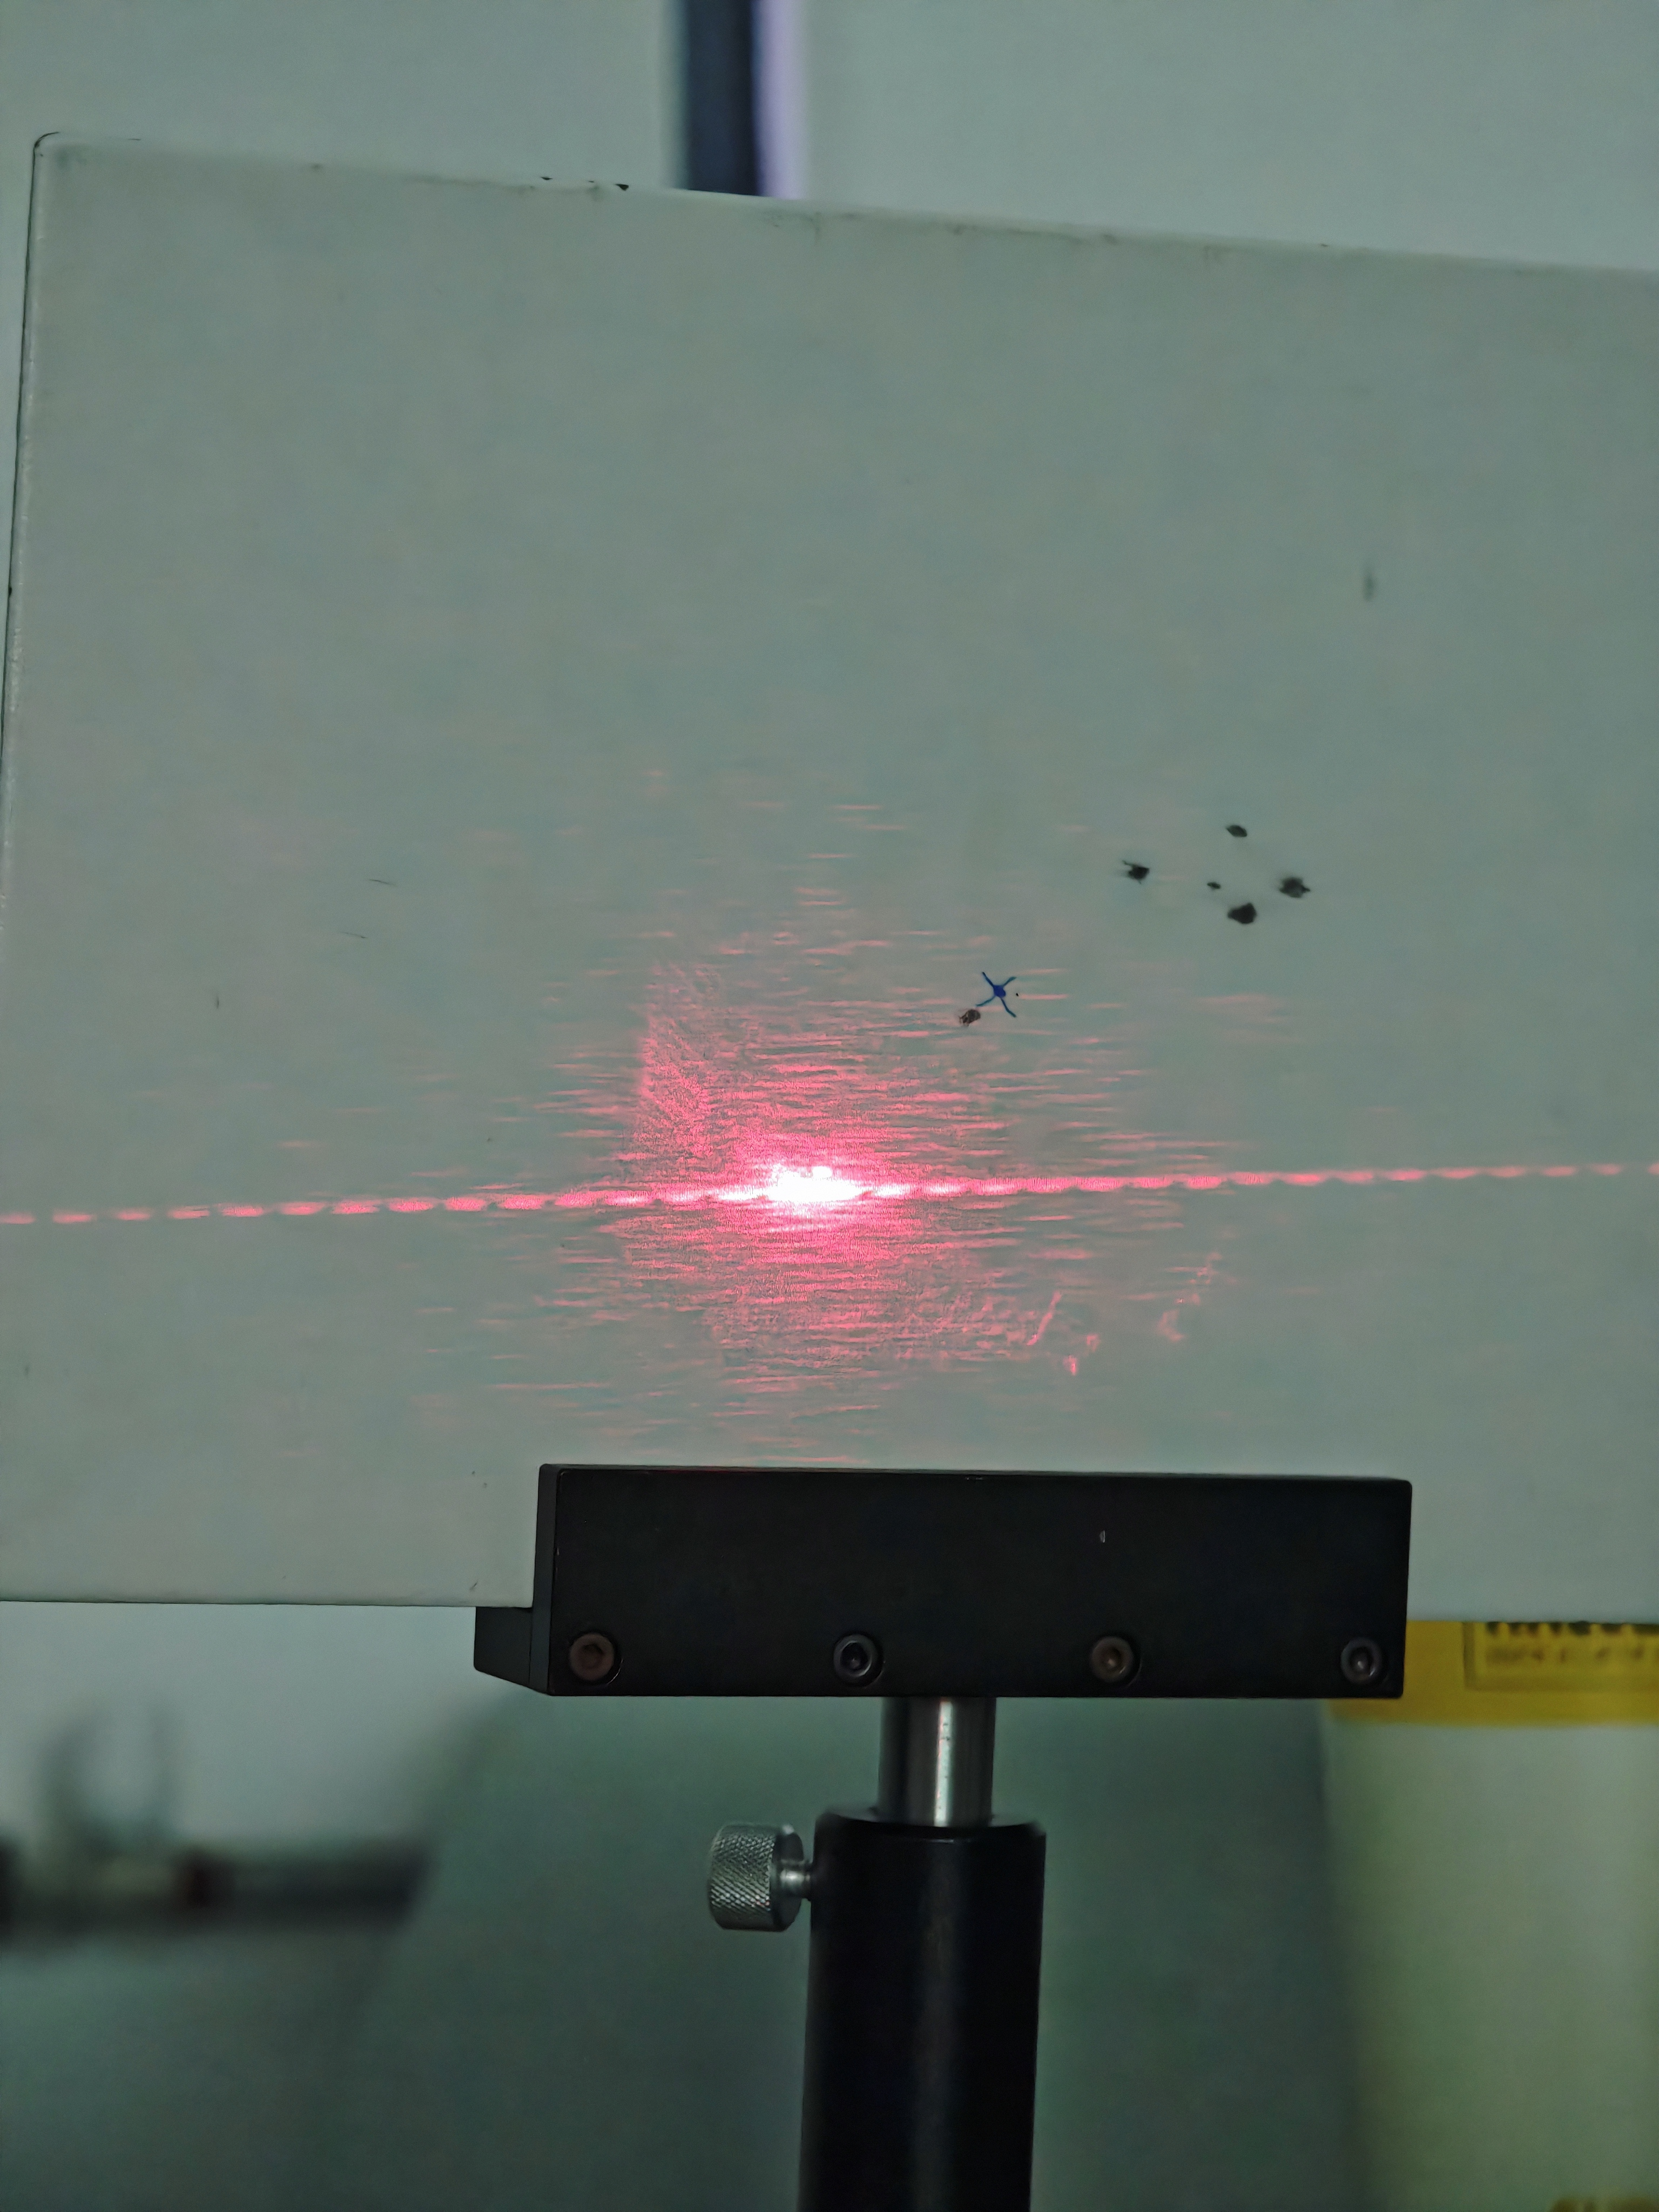
\includegraphics[width=0.24\textwidth]{fig/IMG_20251105_165912.jpg}}
    \subfigure[]{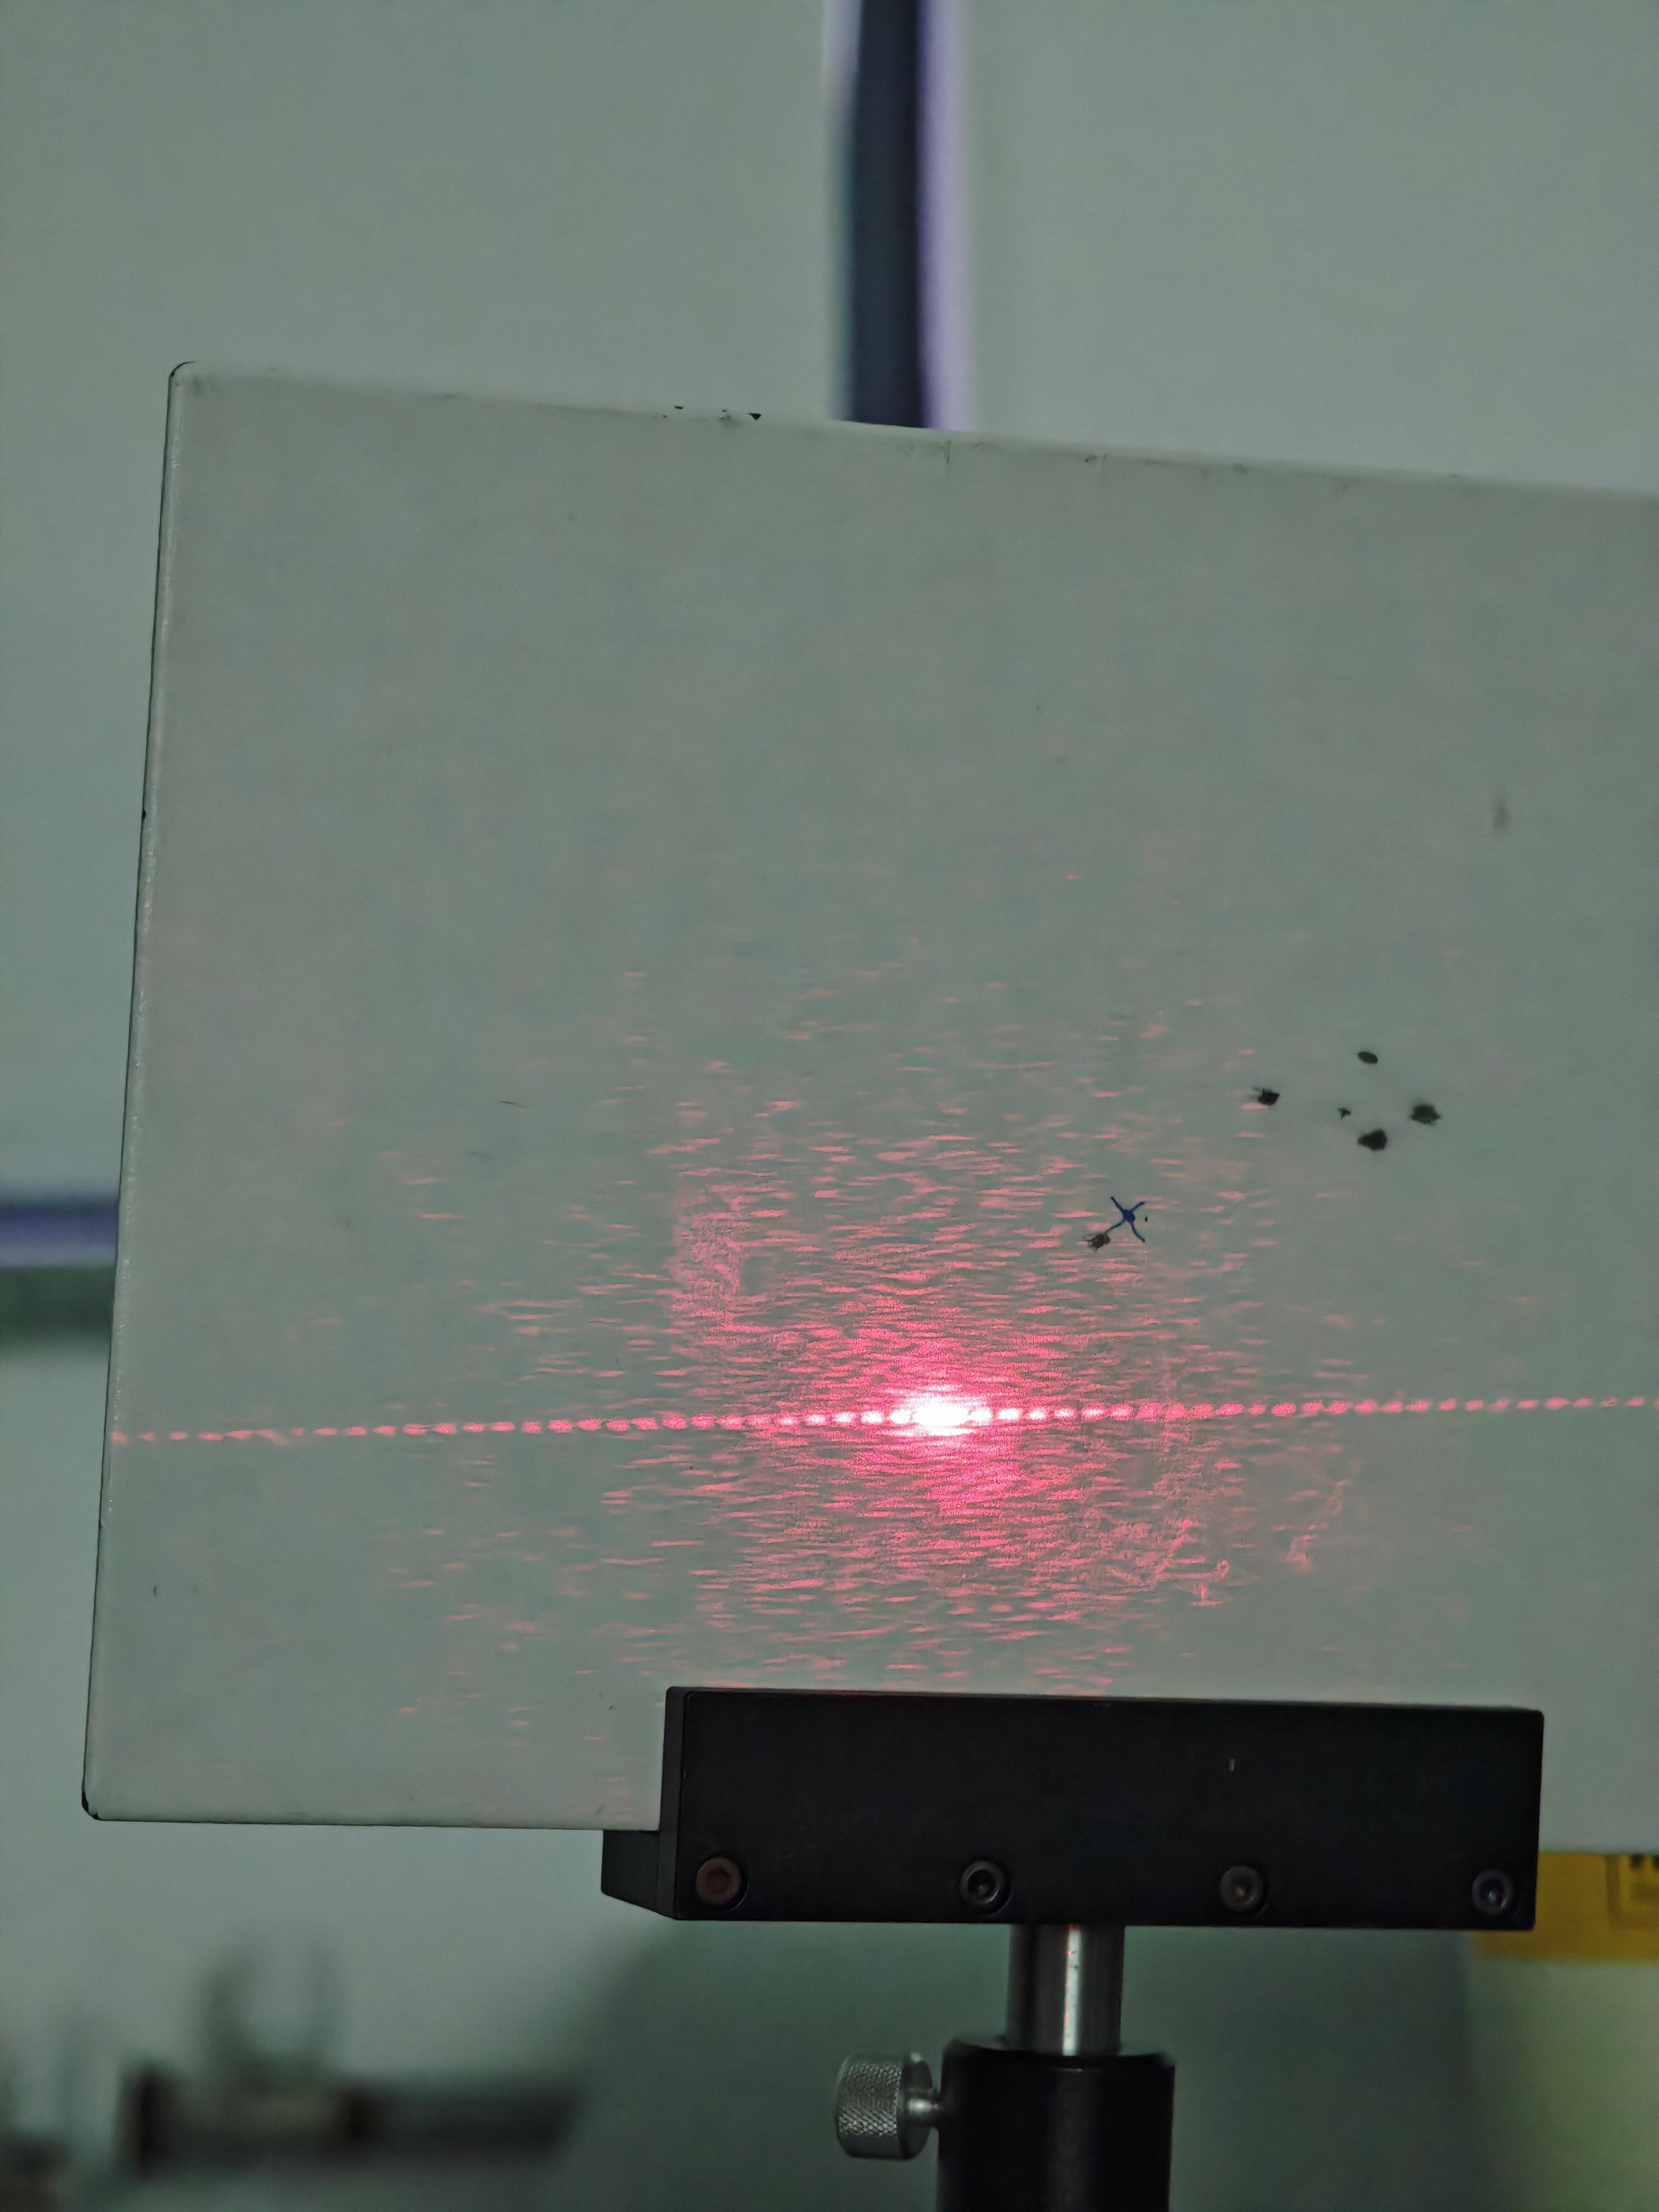
\includegraphics[width=0.24\textwidth]{fig/IMG_20251105_165917.jpg}}
    \subfigure[]{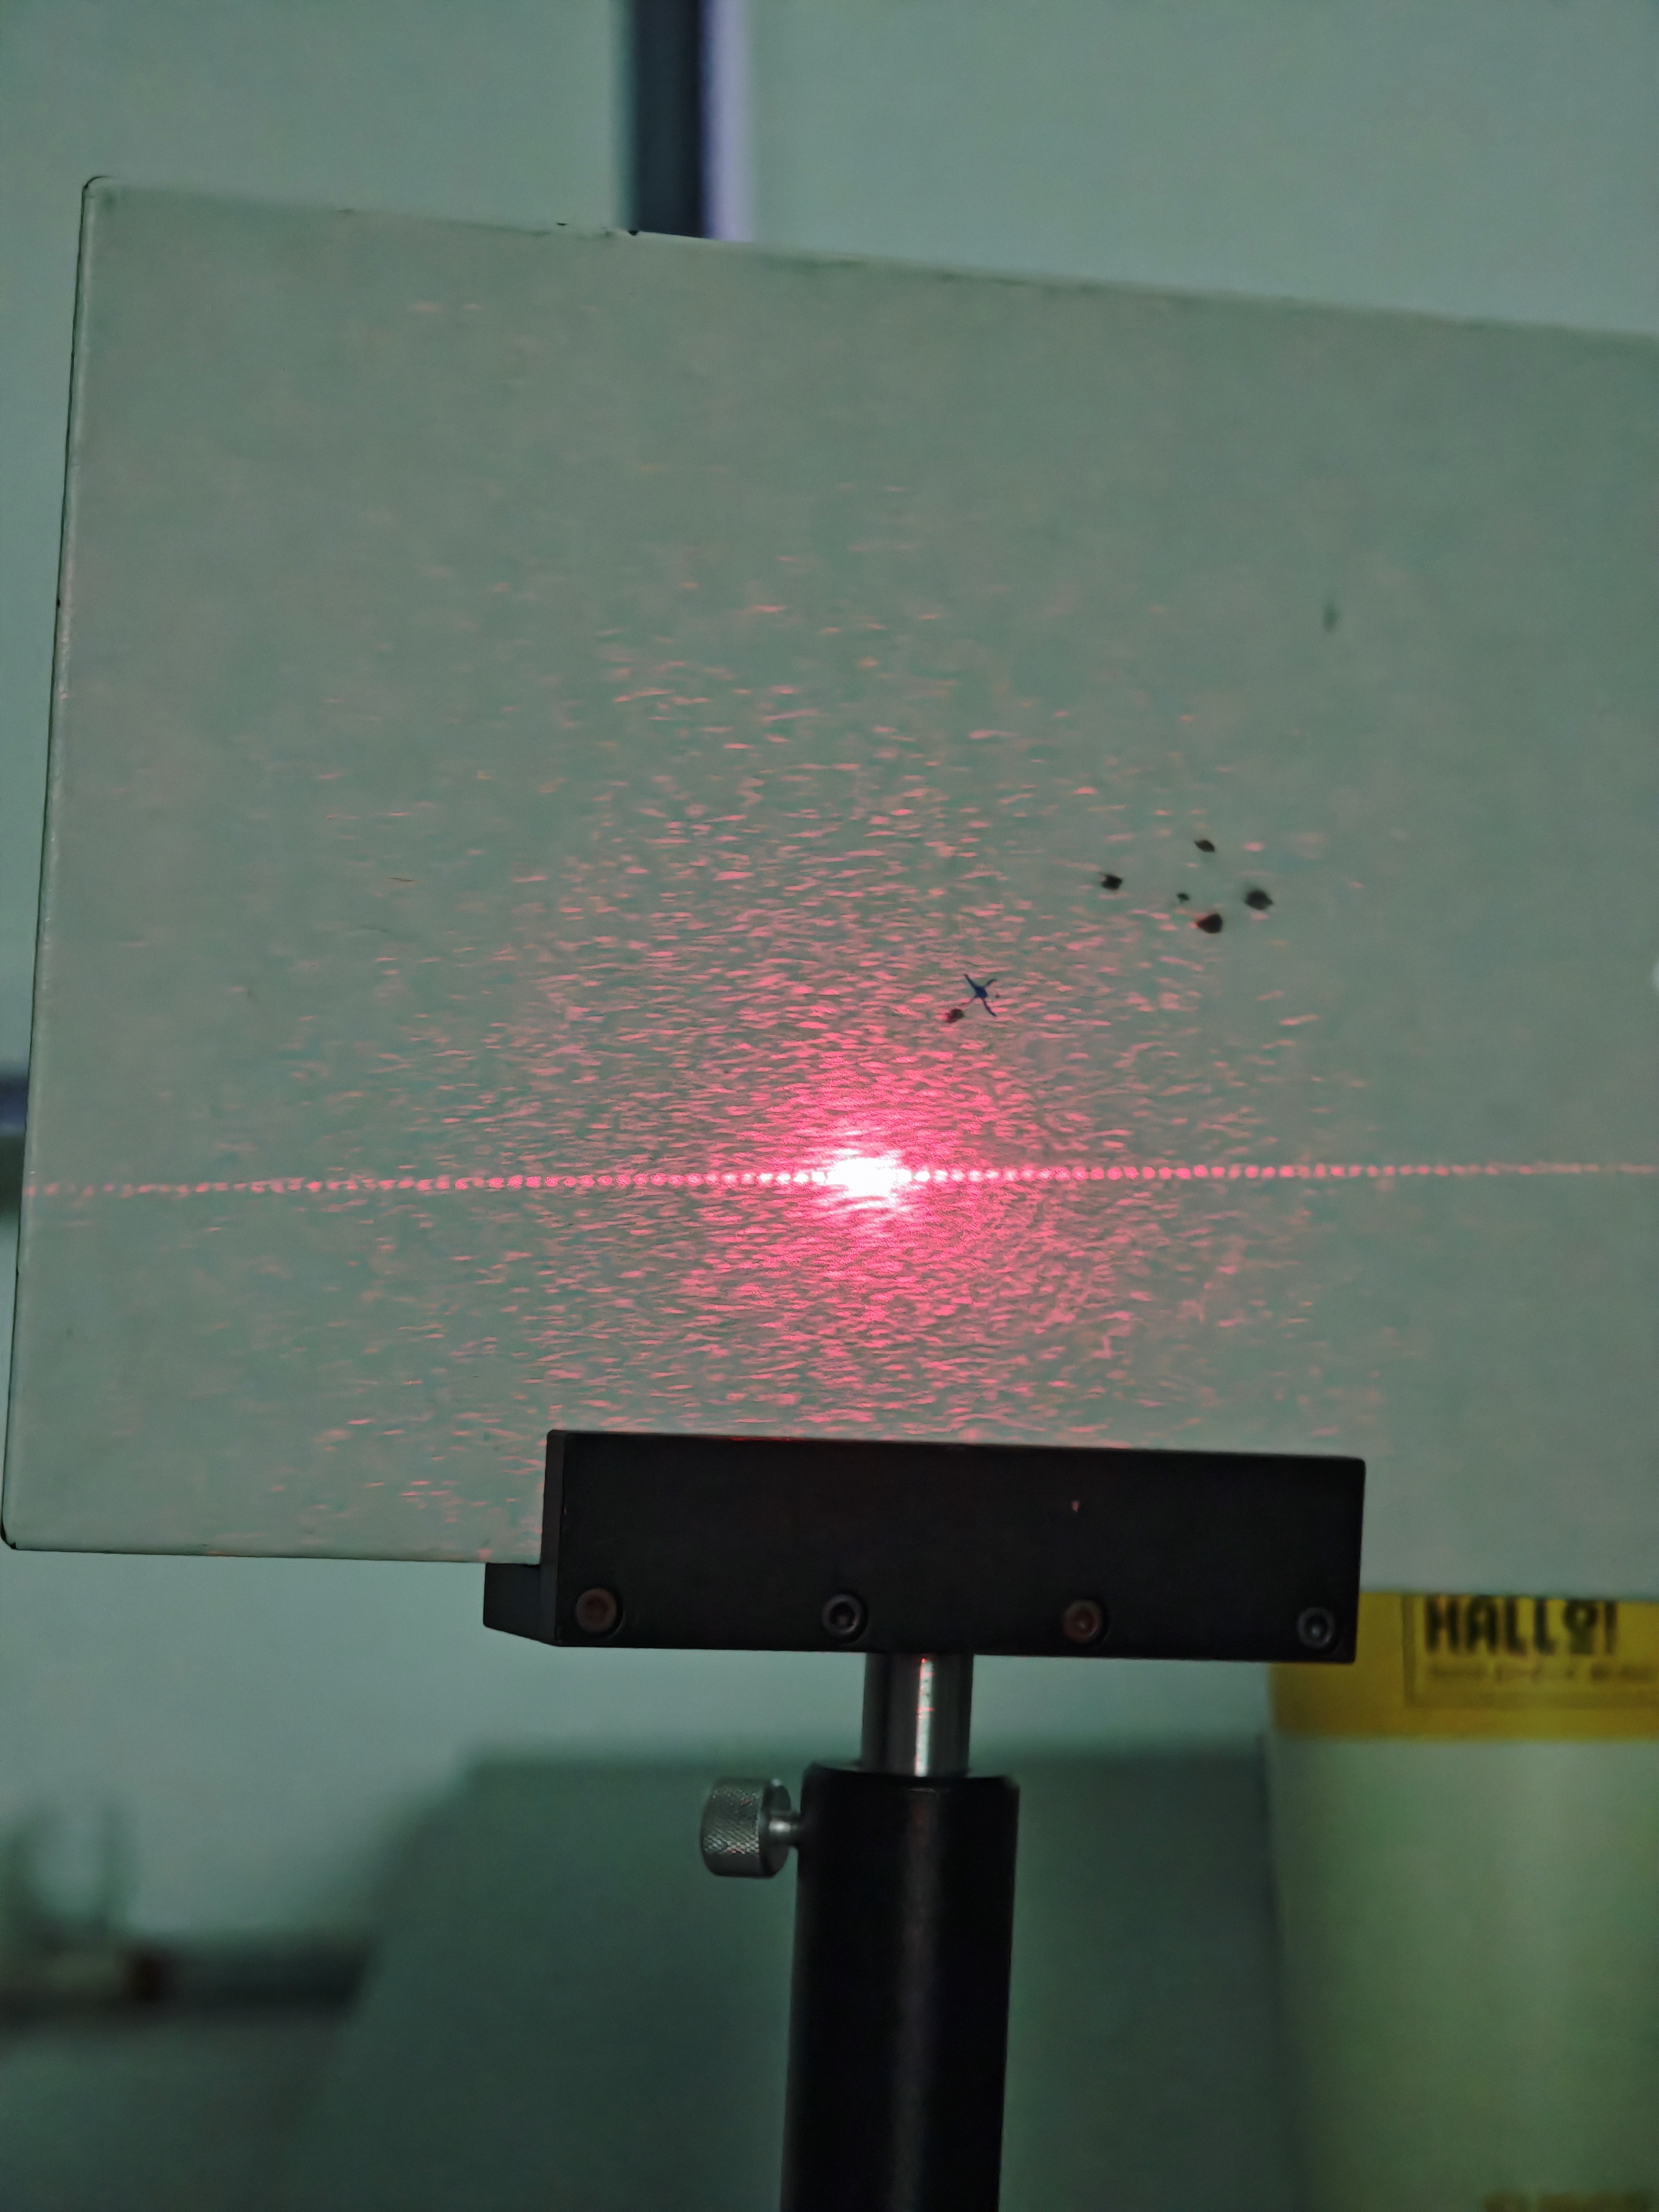
\includegraphics[width=0.24\textwidth]{fig/IMG_20251105_165929.jpg}}
    \subfigure[]{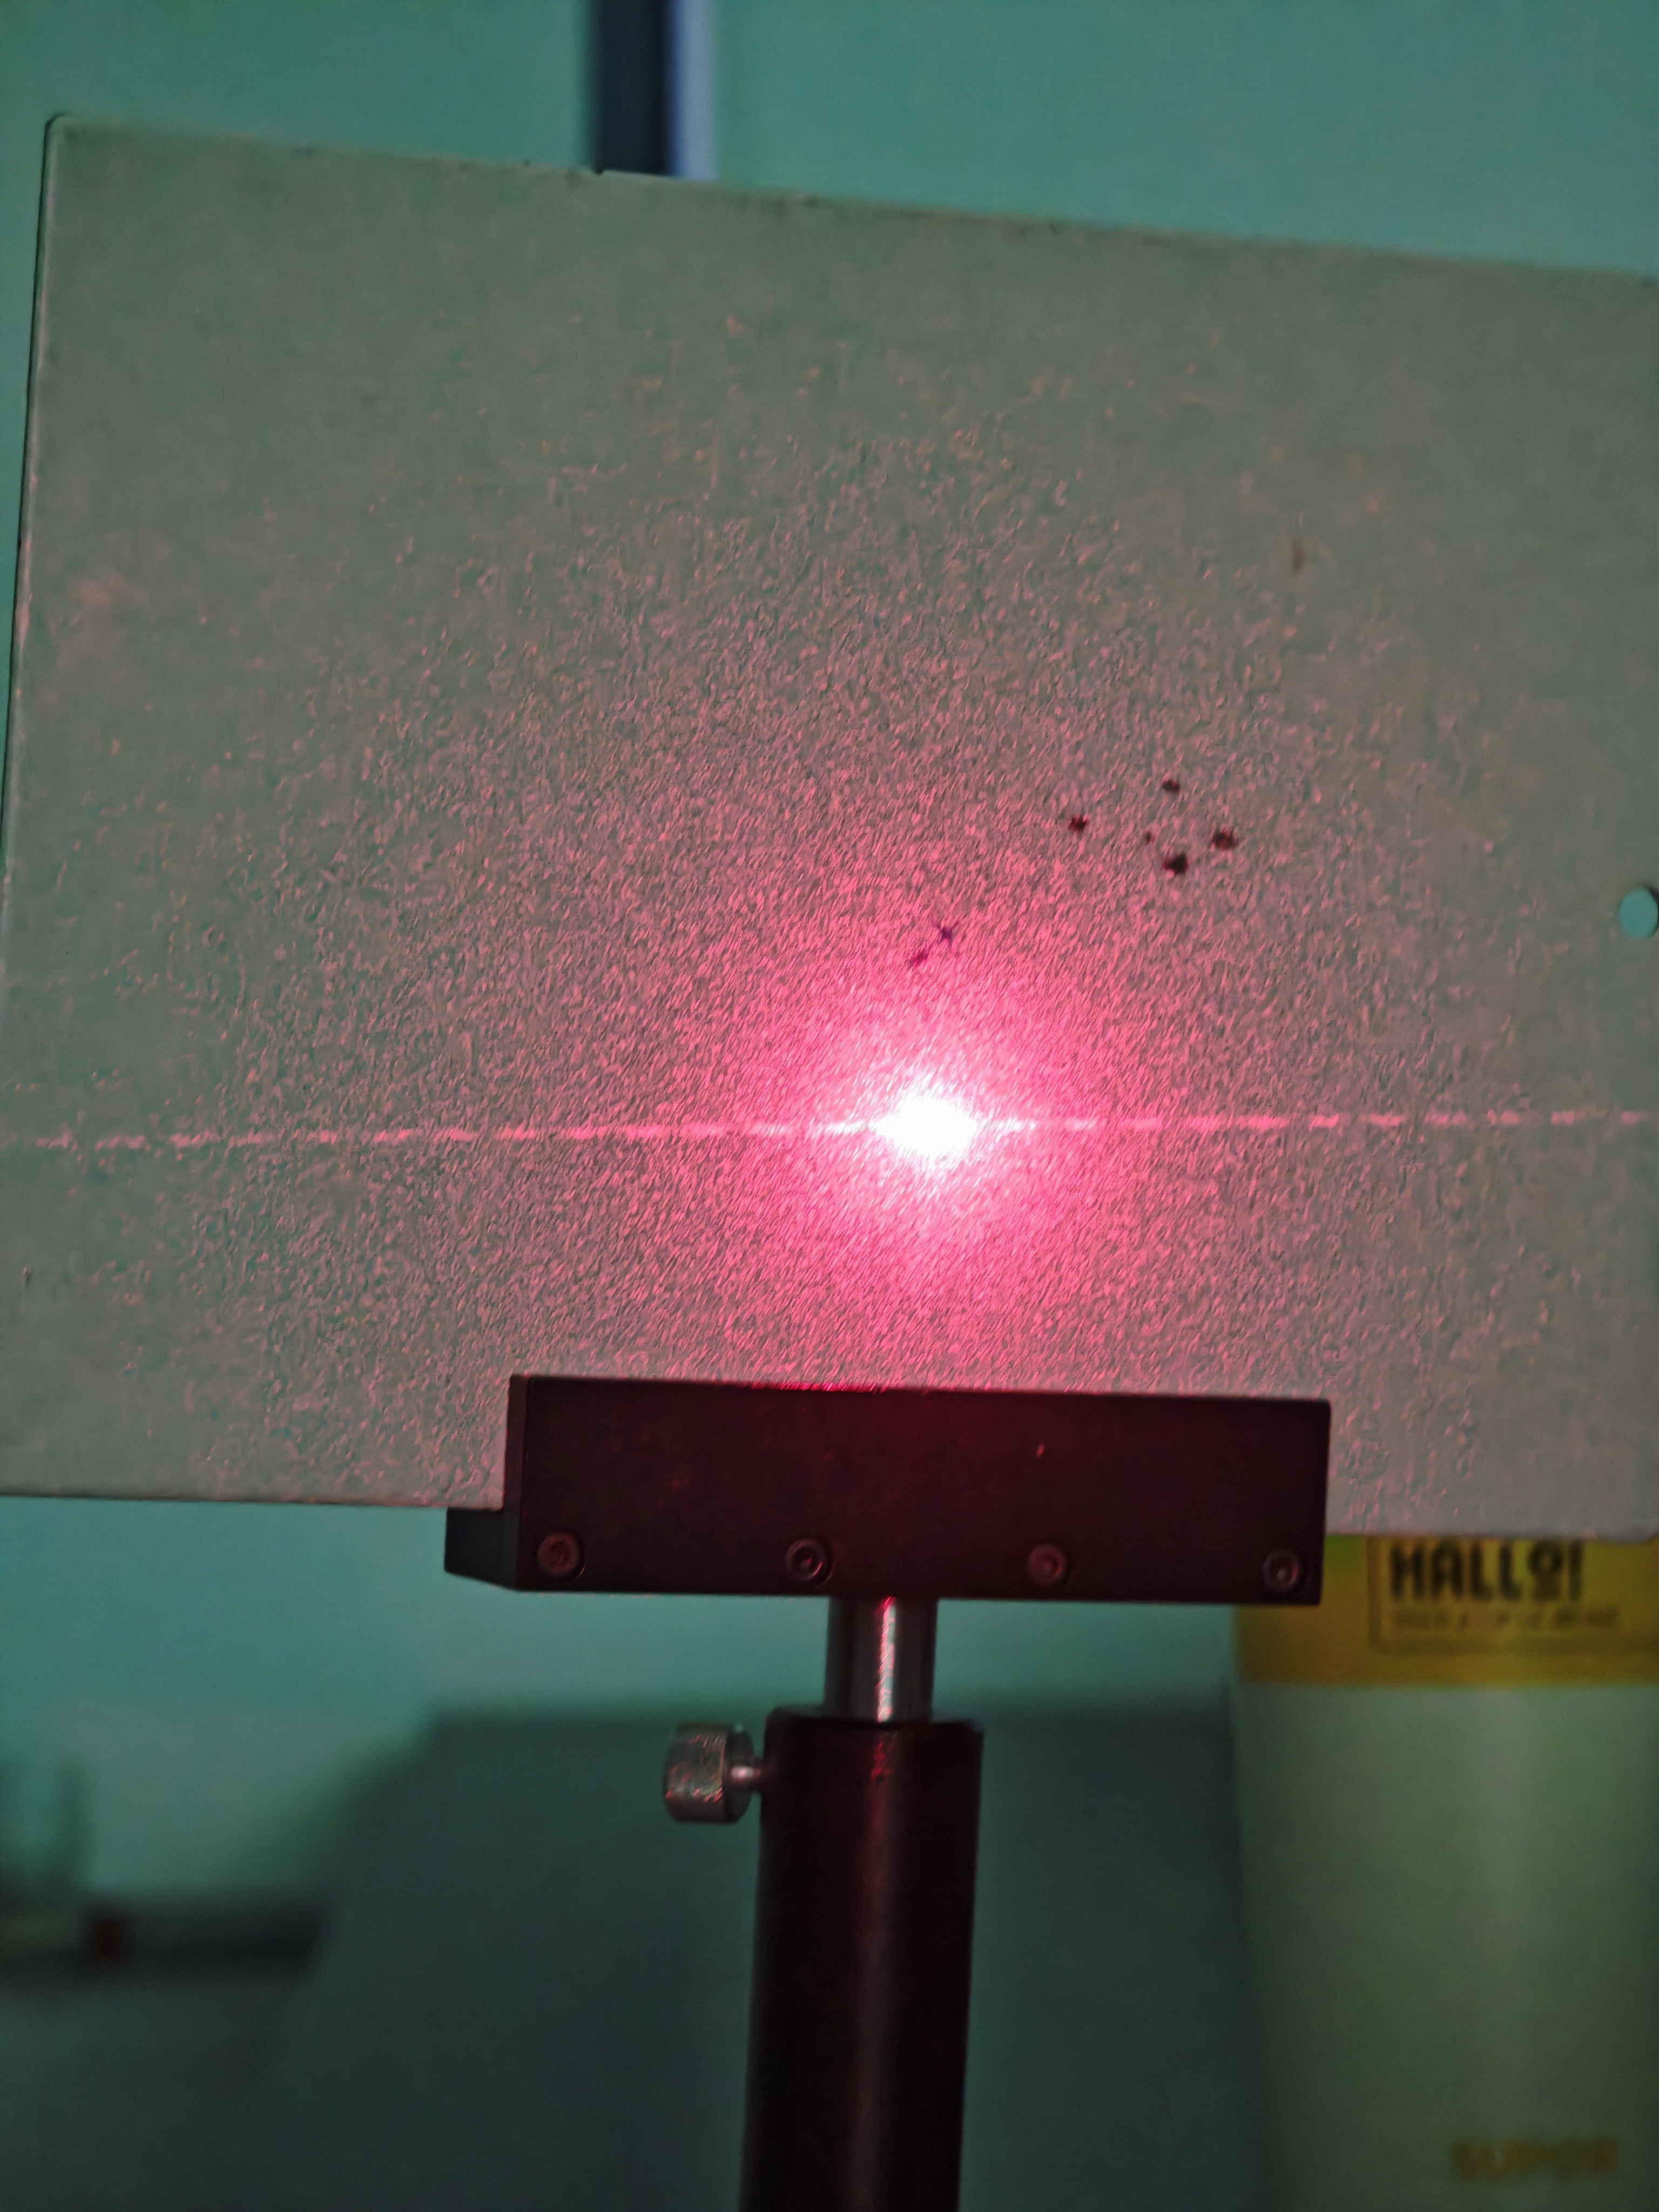
\includegraphics[width=0.24\textwidth]{fig/IMG_20251105_165935.jpg}}
    \subfigure[]{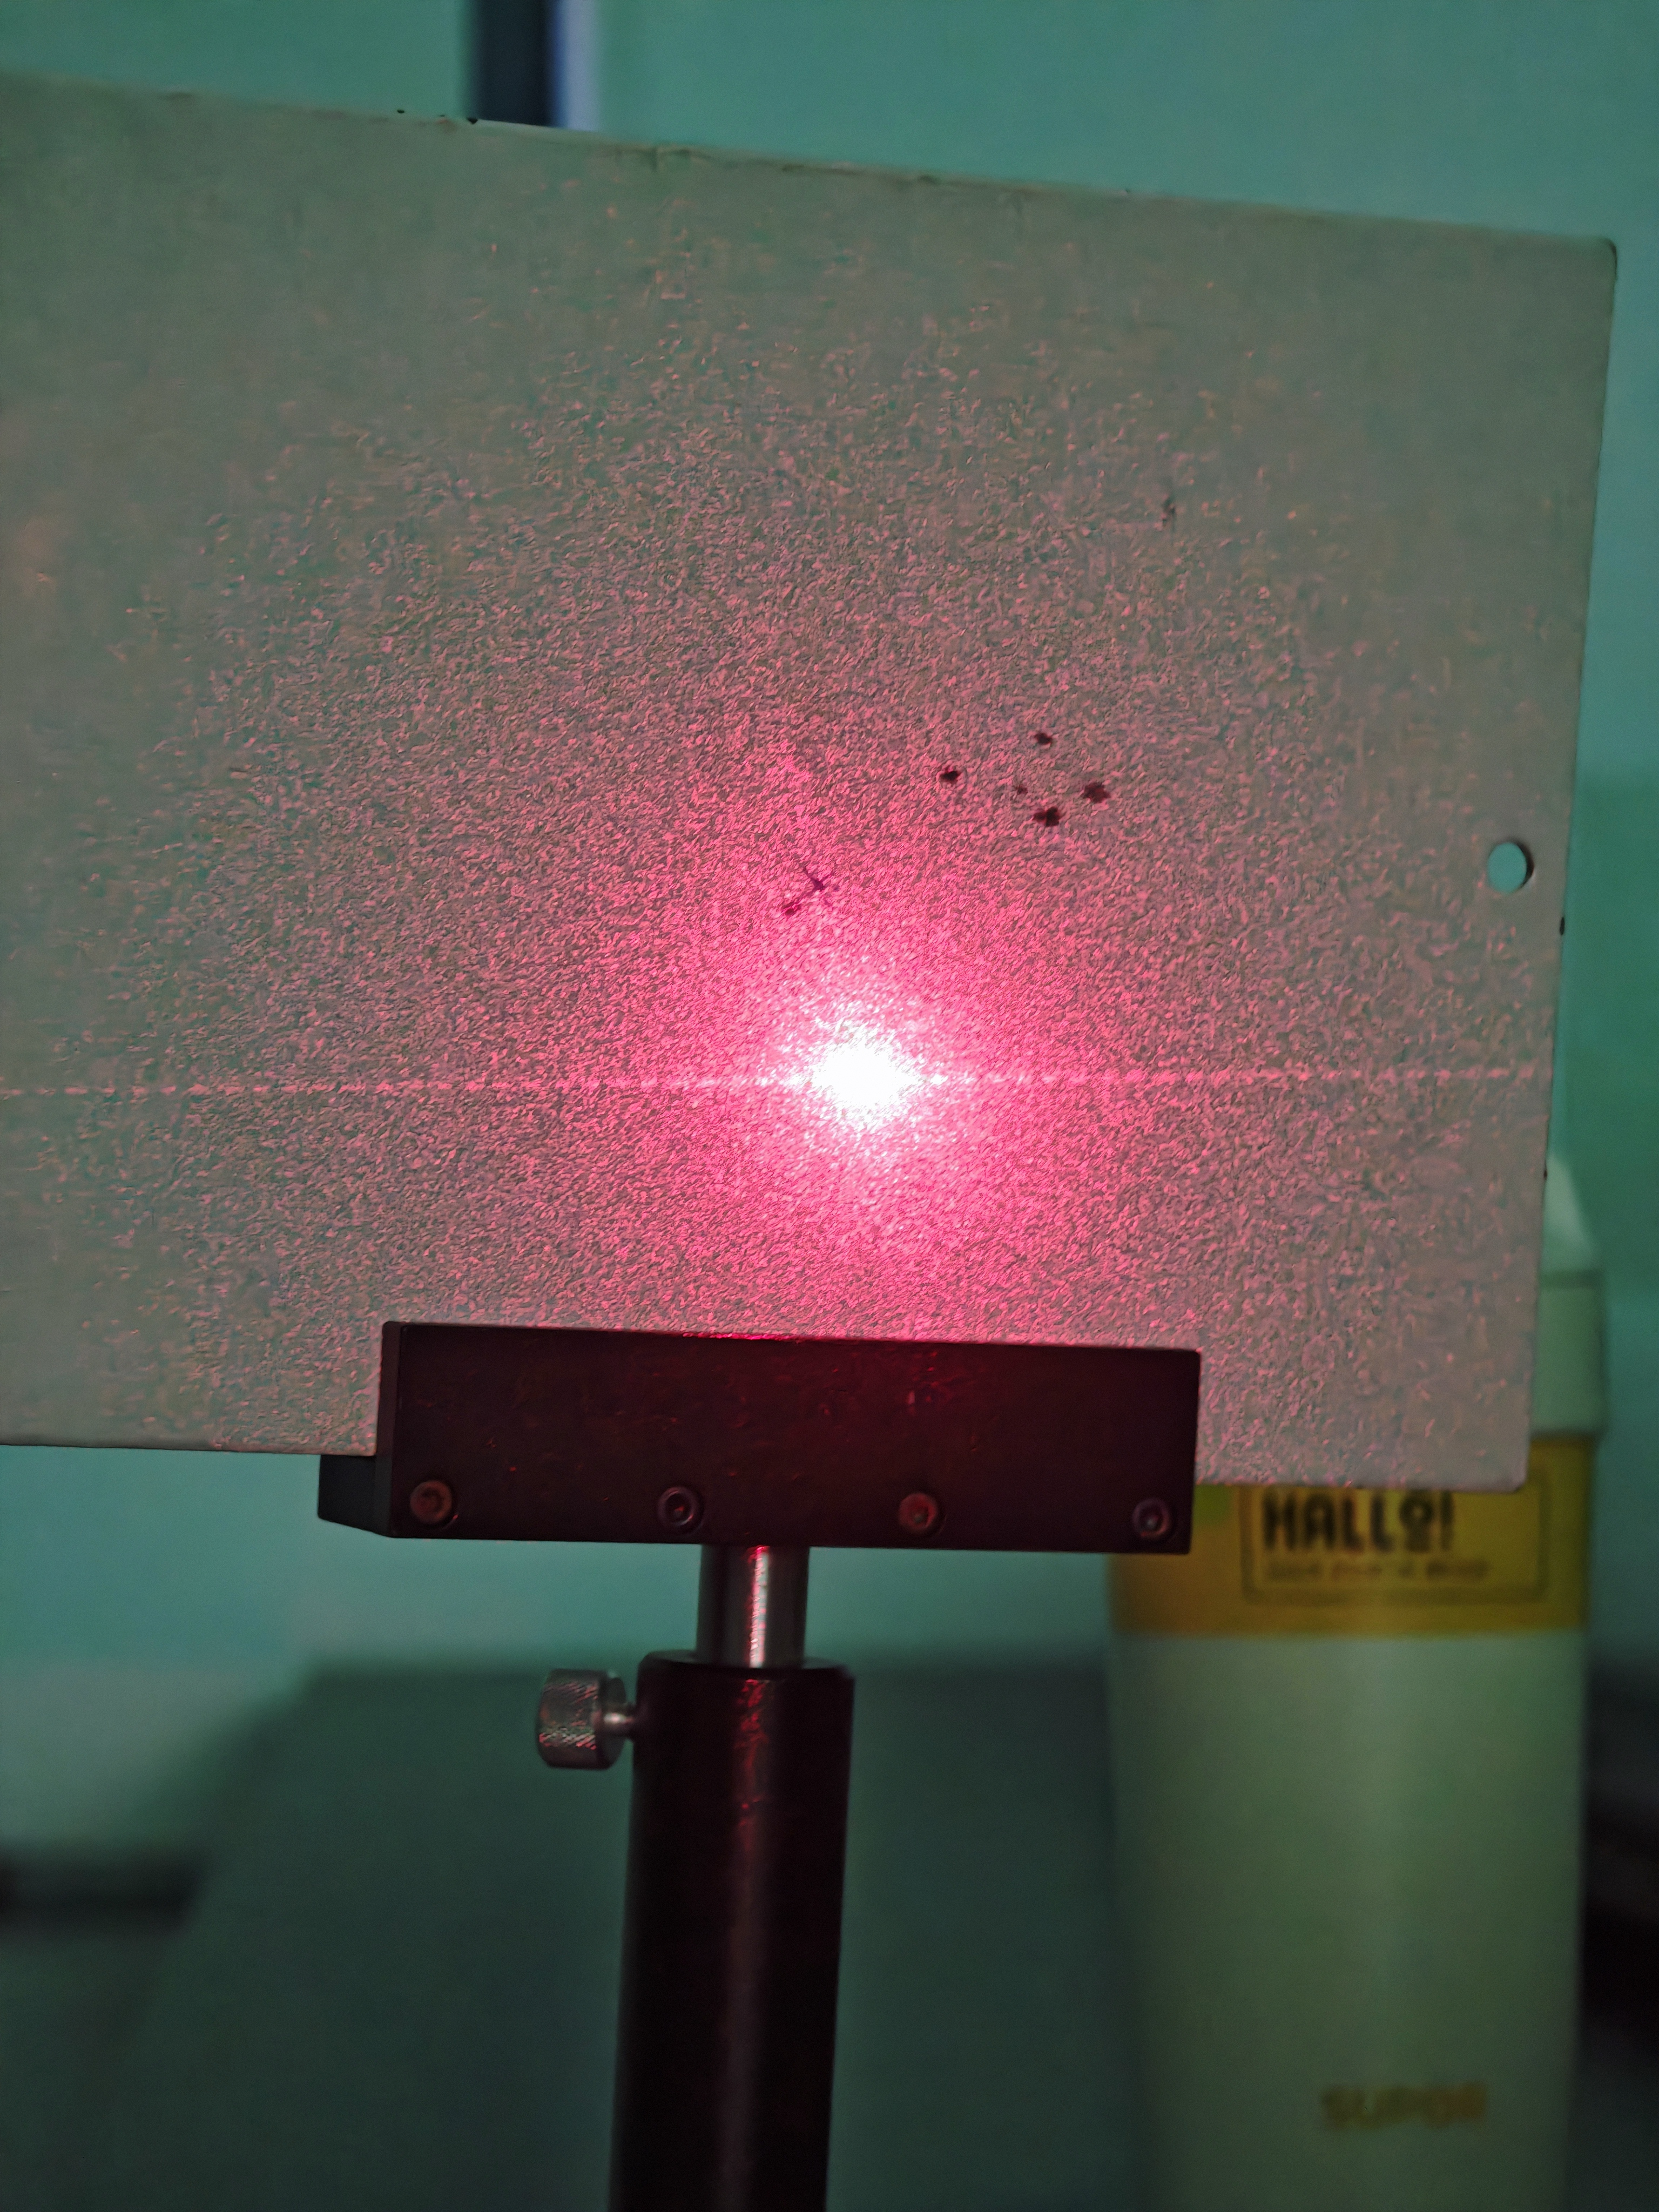
\includegraphics[width=0.24\textwidth]{fig/IMG_20251105_165939.jpg}}
    \subfigure[]{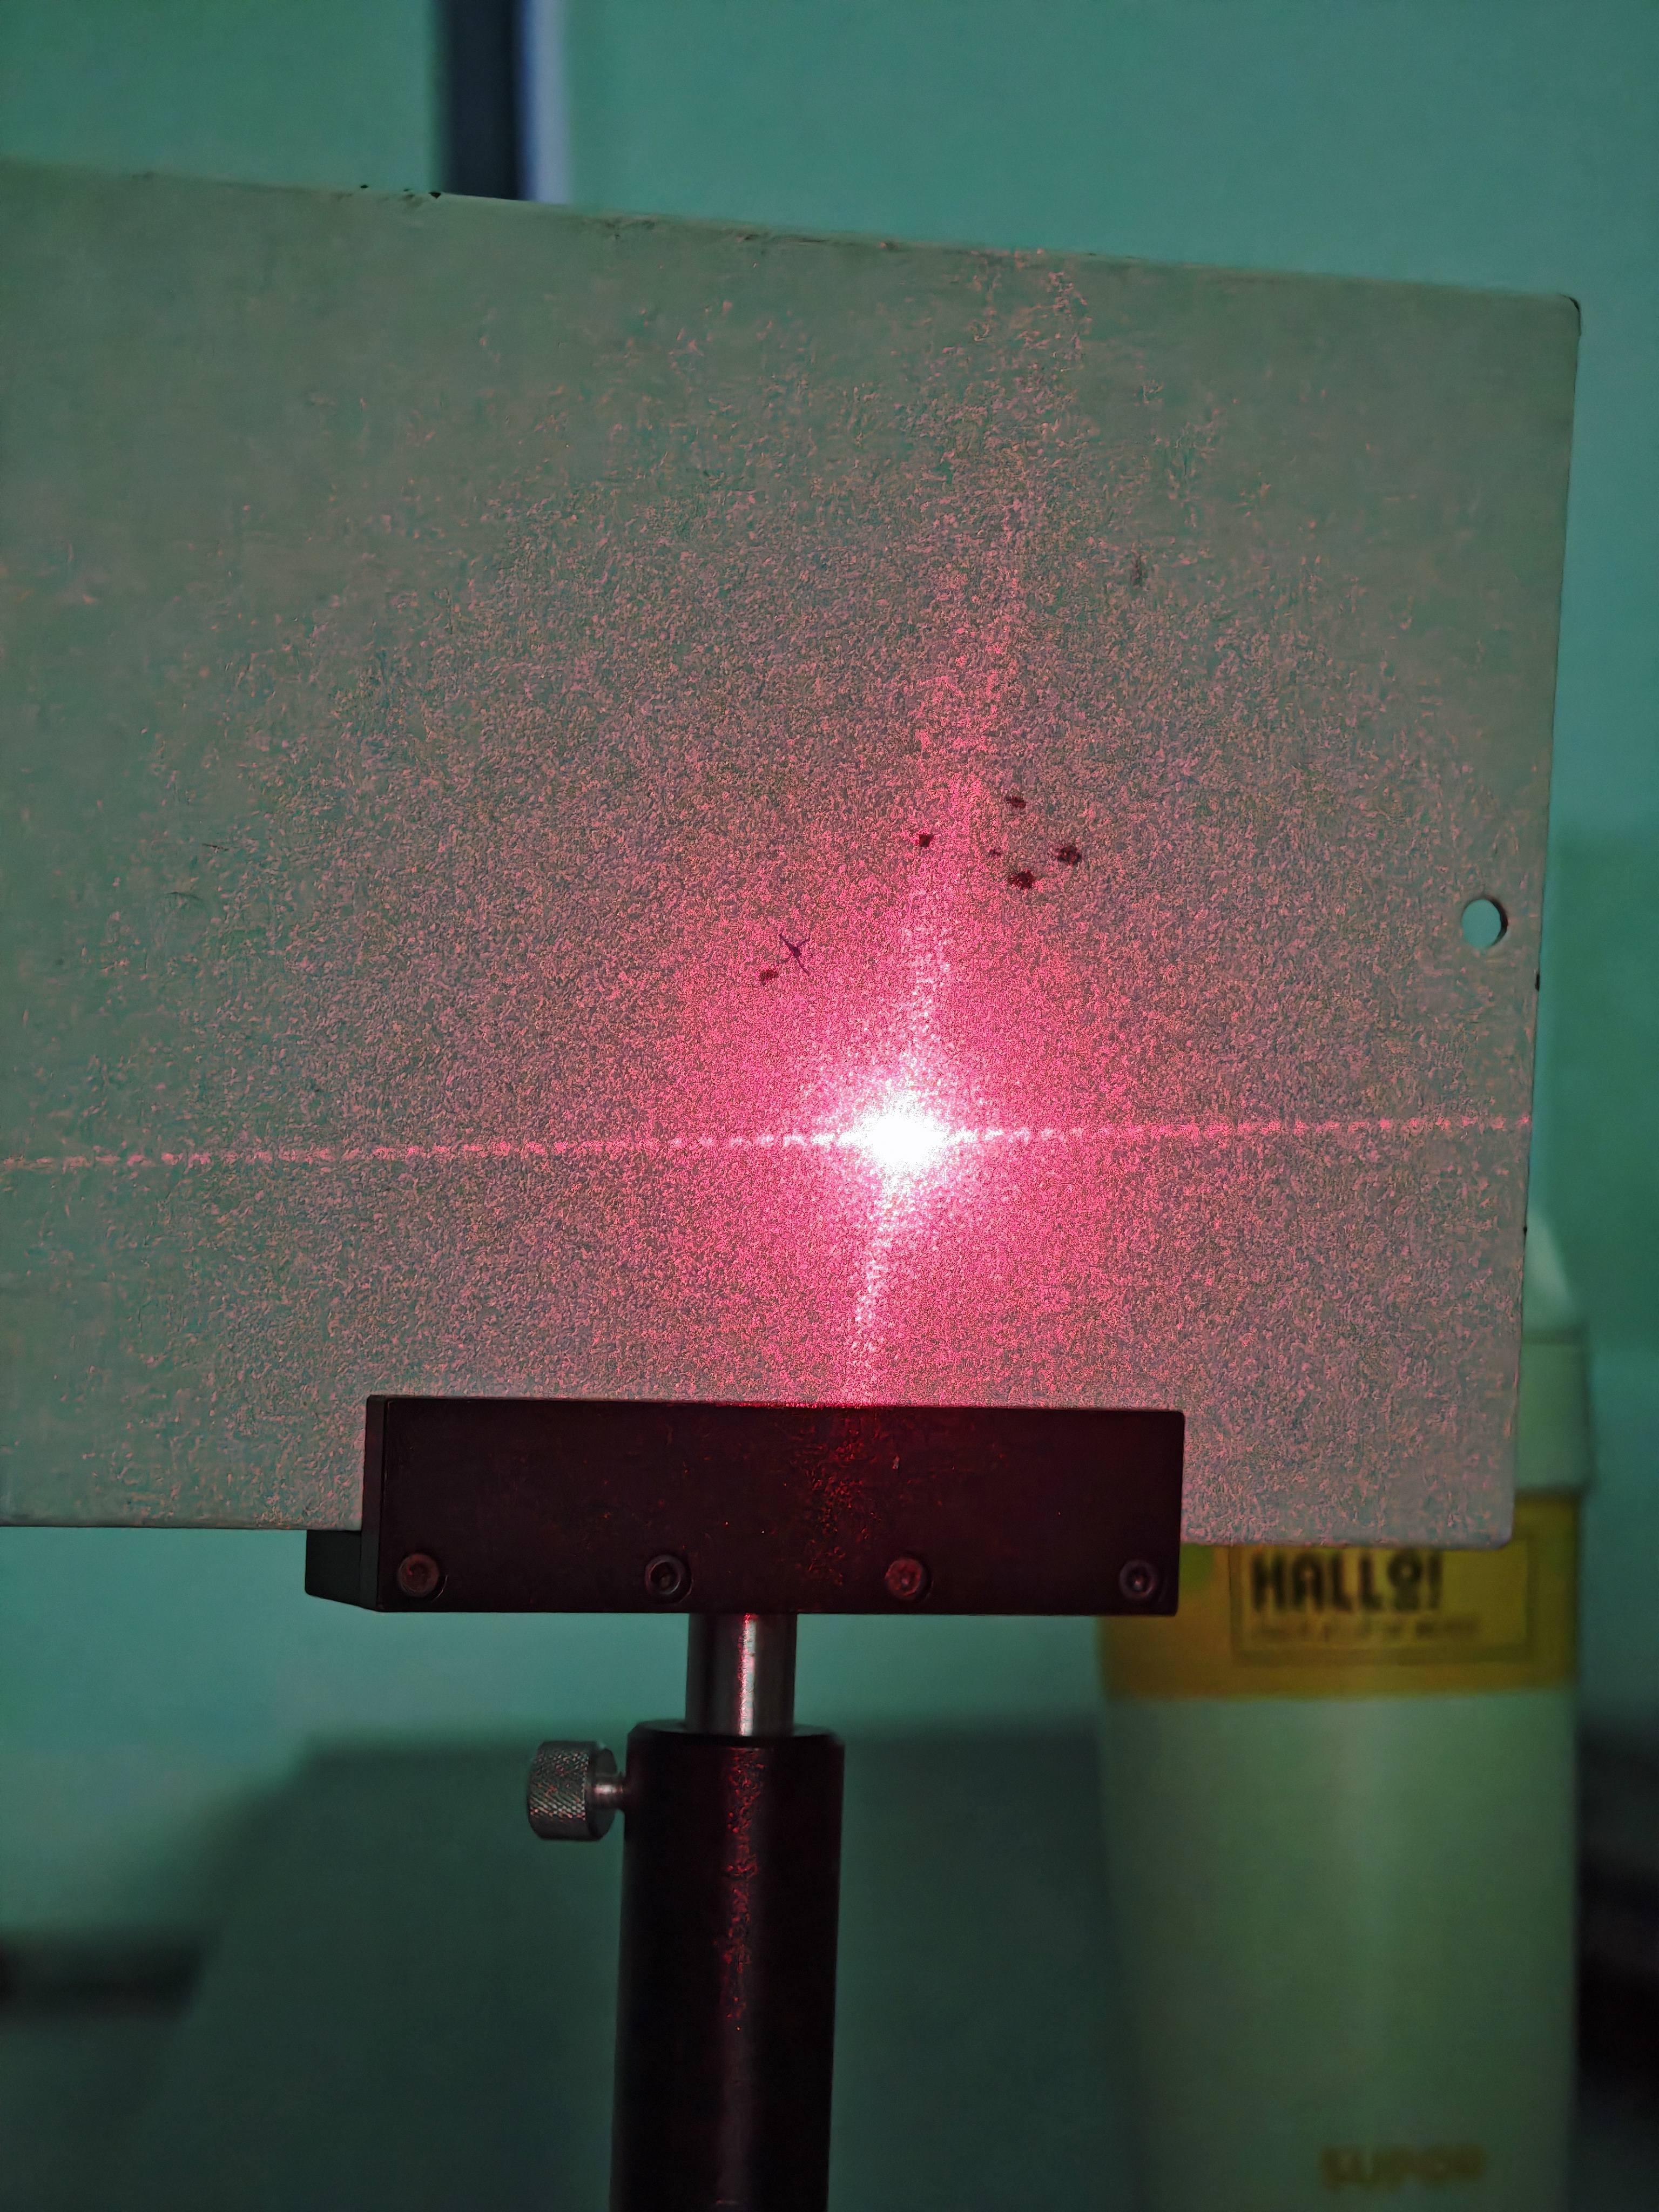
\includegraphics[width=0.24\textwidth]{fig/IMG_20251105_165942.jpg}}
    \caption{夫琅和费衍射与菲涅尔衍射实验结果图3}
\end{figure}

\clearpage

\section{思考题解答}

\subsection*{1) 阿贝成像与滤波相关问题}
\subsubsection*{a) 缝与光栅方向夹角45°滤波的效果}
阿贝成像中，光栅的频谱是沿光栅周期方向分布的离散谱点（如正交光栅的频谱沿 $x, y$ 轴分布）。当滤波“缝”与光栅方向呈45°放置时，仅允许与缝方向一致的频谱分量通过，会对图像的空间频率成分进行选择性过滤：
\begin{itemize}
    \item 若光栅为正交光栅，原频谱沿 $x, y$ 轴分布，45°缝会滤除原主轴方向的频谱，仅保留45°方向的高频分量；
    \item 成像结果会呈现沿45°方向的细节增强（或原方向细节丢失），图像会出现沿缝方向的条纹或纹理特征。
\end{itemize}


\subsubsection*{b) 高通滤波的实现与效果}
\textbf{实现方法}：在频谱面（阿贝成像的物镜后焦面）放置“中心遮挡物”（如小圆盘），遮挡0级斑（低频分量），仅允许高频分量通过。

\textbf{效果}：0级斑对应图像的直流分量（整体亮度、大面积均匀区域），高通滤波会滤除低频、保留边缘/细节的高频信息，因此成像结果为：
\begin{itemize}
    \item 图像整体亮度降低，大面积均匀区域变暗；
    \item 物体的边缘、轮廓、细节（如光栅的栅线）会被增强显示。
\end{itemize}


\subsection*{2) 4F系统成像与阿贝成像（单透镜）的区别}
\begin{table}[!ht]
    \centering
    \begin{tabular}{|p{0.45\textwidth}|p{0.45\textwidth}|}
        \hline
        \textbf{4F系统成像} & \textbf{阿贝成像（单透镜）} \\
        \hline
        由两个透镜组成（输入面 $\rightarrow$ L1 $\rightarrow$ 频谱面 $\rightarrow$ L2 $\rightarrow$ 像面），满足“物面到L1距离=$f$，L1到频谱面距离=$f$；频谱面到L2距离=$f$，L2到像面距离=$f$”，是严格的傅里叶变换系统。 & 由单个透镜完成成像，物面位于透镜物方焦面附近，像面为透镜的像方空间，频谱面为透镜后焦面，是“成像+频谱分析”的结合。 \\
        \hline
        频谱面位置固定（L1与L2的共焦面），滤波操作（如遮挡、选通）更灵活、精准。 & 频谱面为透镜后焦面，但像面与频谱面的距离由物距决定，操作相对受限。 \\
        \hline
        核心功能是“傅里叶变换 $\rightarrow$ 滤波 $\rightarrow$ 逆变换”，是信号处理的典型光学系统。 & 核心是“成像过程的频谱分解”，用于展示成像的物理本质。 \\
        \hline
    \end{tabular}
\end{table}


\subsection*{3) 假彩色编码中门窗变黑的原因及验证}
\textbf{原因}：天安门城楼光栅中，门窗是“透光区域”，但该区域的光栅周期（或空间频率）与背景不同；假着色滤波片是“频率选择型滤光片”，仅允许背景区域的频谱分量通过，而门窗区域的频谱被滤波片阻挡，因此成像时门窗区域无光通过，呈现黑色。

\textbf{验证方法}：
\begin{itemize}
    \item 将滤波片替换为“全透光片”，观察成像：此时门窗区域应恢复透光（明亮）；
    \item 单独提取门窗区域的光栅，测量其空间频率，对比滤波片的通带频率：若门窗频率不在通带内，则验证了“频率过滤”的解释。
\end{itemize}


\subsection*{4) 夫琅禾费衍射的规律}
夫琅禾费衍射（平行光入射、远场接收）的核心规律：
\begin{enumerate}
    \item 单缝衍射：
          衍射图样为“中央亮斑（最宽最亮）+ 两侧交替明暗纹”，
          暗纹位置满足：$a\sin\theta = k\lambda$（$a$为缝宽，$\theta$为衍射角，$k=\pm1,\pm2,\dots$）；
          缝宽 $a$ 越小，衍射图样越展宽。

    \item 圆孔衍射：
          衍射图样为“艾里斑（中央亮斑）+ 同心圆环”，
          艾里斑角半径：$\theta_0 = 1.22\frac{\lambda}{D}$（$D$为圆孔直径）；
          是光学仪器分辨率的理论基础（瑞利判据）。

    \item 光栅衍射：
          衍射图样为“细锐亮纹+暗区”，是“单缝衍射调制下的多缝干涉”；
          主极大位置满足：$d\sin\theta = k\lambda$（$d$为光栅常数）；
          光栅常数 $d$ 越小、缝数越多，亮纹越细锐。

    \item 共性规律：
          衍射图样的展宽程度与入射波长 $\lambda$ 成正比，与衍射单元尺寸（缝宽、圆孔直径）成反比；
          是“波的相干叠加”的直接体现。
\end{enumerate}

\end{document}